\documentclass[a4paper, 10pt]{article}
\usepackage[margin=1in]{geometry}
\usepackage{amsfonts, amsmath, amssymb, amsthm}
\usepackage[none]{hyphenat}
\usepackage{fancyhdr} %create a custom header and footer
\usepackage[utf8]{inputenc}
\usepackage[english, main=ukrainian]{babel}
\usepackage{pgfplots}
\usepgfplotslibrary{fillbetween}
\usepackage{bm}
\usepackage{physics}
\usepackage[unicode]{hyperref}
\usepackage{scalerel,stackengine}
\usepackage{multicol}
\usepackage{tikz-cd}
\usetikzlibrary{fit,matrix}
\usepackage{graphicx}

\usepackage{pdfpages}
\usepackage{caption}
\usepackage{float}
\usepackage{physics}
\usetikzlibrary{spy}

\fancyhead{}
\fancyfoot{}
\parindent 0ex

\def\rightproof{$\boxed{\Rightarrow}$ }

\def\leftproof{$\boxed{\Leftarrow}$ }

\newtheoremstyle{theoremdd}% name of the style to be used
  {\topsep}% measure of space to leave above the theorem. E.g.: 3pt
  {\topsep}% measure of space to leave below the theorem. E.g.: 3pt
  {\normalfont}% name of font to use in the body of the theorem
  {0pt}% measure of space to indent
  {\bfseries}% name of head font
  {}% punctuation between head and body
  { }% space after theorem head; " " = normal interword space
  {\thmname{#1}\thmnumber{ #2}\textnormal{\thmnote{ \textbf{#3}\\}}}

\theoremstyle{theoremdd}
\newtheorem{theorem}{Theorem}[subsection]
\newtheorem{definition}[theorem]{Definition}
\newtheorem{example}[theorem]{Example}
\newtheorem{proposition}[theorem]{Proposition}
\newtheorem{remark}[theorem]{Remark}
\newtheorem{lemma}[theorem]{Lemma}
\newtheorem{corollary}[theorem]{Corollary}

\newcommand\thref[1]{\textbf{Th.~\ref{#1}}}
\newcommand\defref[1]{\textbf{Def.~\ref{#1}}}
\newcommand\exref[1]{\textbf{Ex.~\ref{#1}}}
\newcommand\prpref[1]{\textbf{Prp.~\ref{#1}}}
\newcommand\rmref[1]{\textbf{Rm.~\ref{#1}}}
\newcommand\lmref[1]{\textbf{Lm.~\ref{#1}}}
\newcommand\crlref[1]{\textbf{Crl.~\ref{#1}}}

\renewcommand{\qedsymbol}{$\blacksquare$}

\makeatletter
\renewenvironment{proof}[1][Proof.\\]{\par
\pushQED{\hfill \qed}%
\normalfont \topsep6\p@\@plus6\p@\relax
\trivlist
\item\relax
{\bfseries
#1\@addpunct{.}}\hspace\labelsep\ignorespaces
}{%
\popQED\endtrivlist\@endpefalse
}
\makeatother
    	
\begin{document}
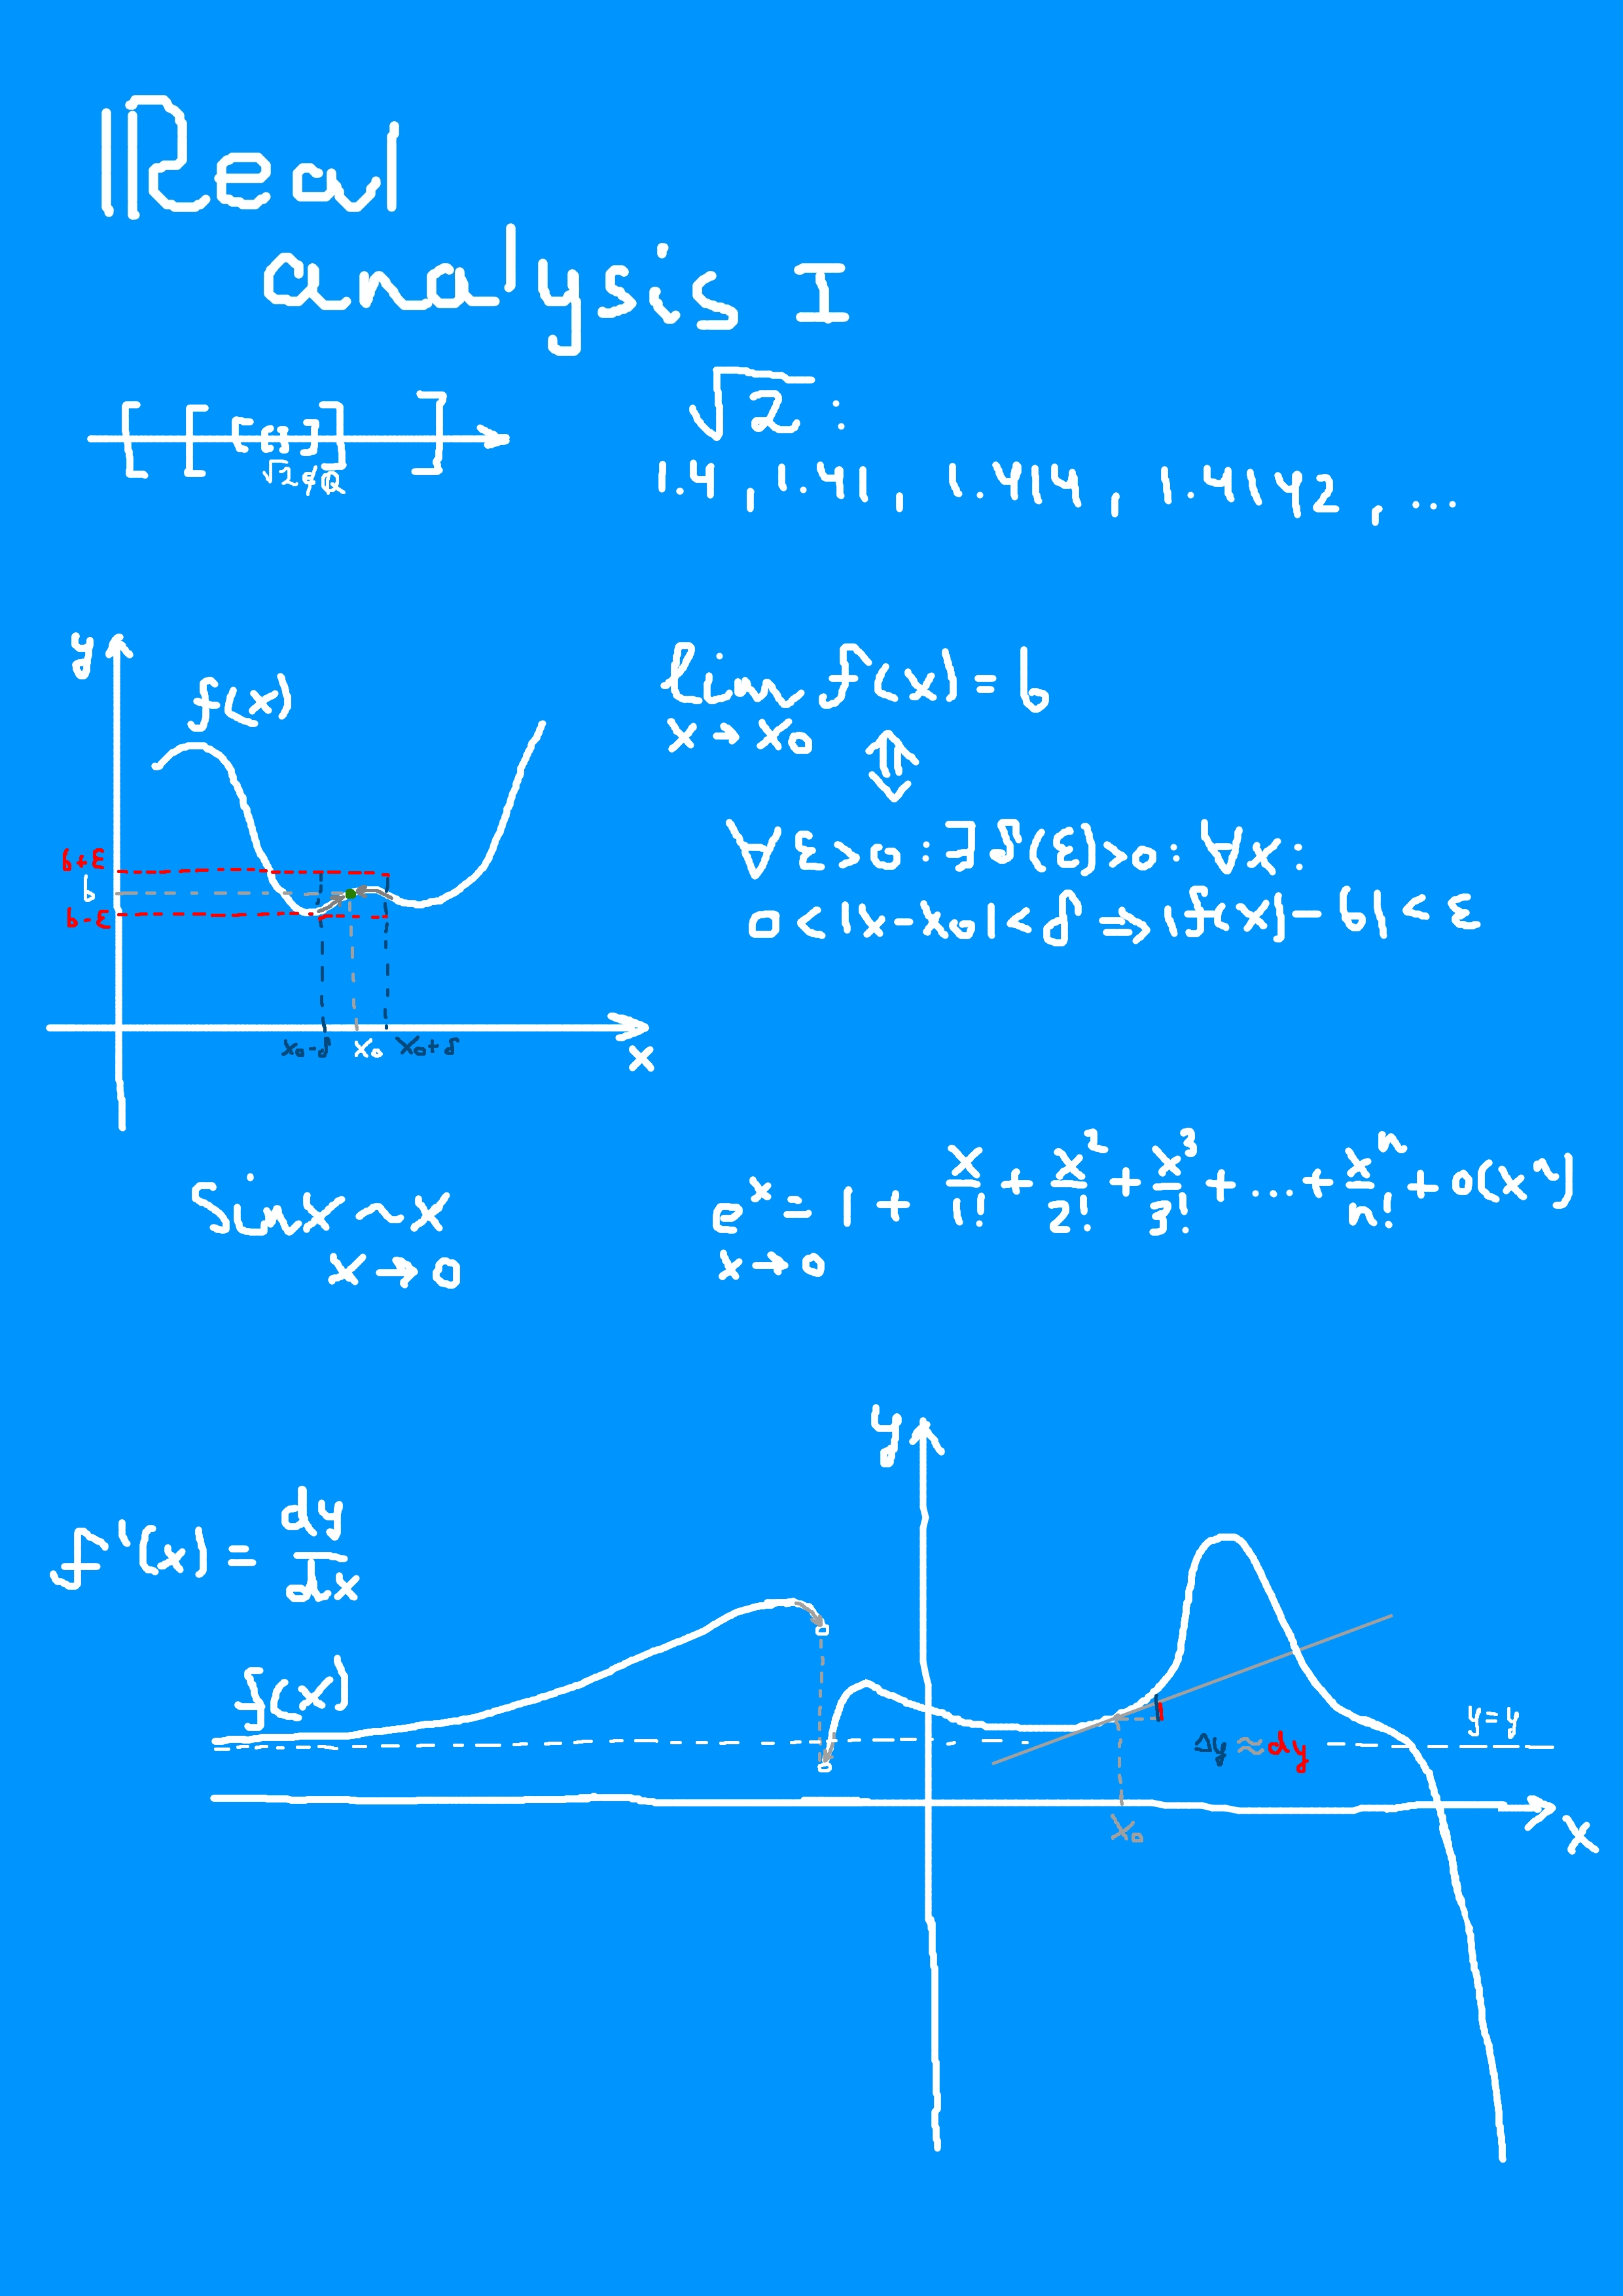
\includepdf[scale=1]{preview.jpg}
\tableofcontents
\newpage
    	
	\section{Лінійні простори}
	\subsection{Основні означення лінійних просторів}
	\begin{definition}\label{linear space}
	\textbf{Лінійним простором} називається множина $L$, на якій задані дві операції:
	\begin{align*}
	\begin{tabular}{cl}
	1. & $\forall x,y \in L: \exists! z \in L: z = x + y$ - операція додавання \\
	2. & $\forall x \in L, \forall \lambda \in \mathbb{R}: \exists! w \in L: w = \lambda x$ - операція множення на скаляр \\
	\end{tabular}
	\end{align*}
	та які задовільняють наступним аксіомам:
	\begin{align*}
	\begin{tabular}{cl}
	1) & $\forall x,y \in L: x + y = y + x$\\
	2) & $\forall x,y,z \in L: (x + y) + z = x + (y + z)$\\
	3) & $\exists 0 \in L: \forall x \in L: x + 0 = x$\\
	4) & $\forall x \in L: \exists \tilde{x} \in L: x + \tilde{x} = 0$\\
	5) & $\forall \alpha, \beta \in \mathbb{R}: \forall x \in L: (\alpha + \beta) x = \alpha x + \beta x$\\
	6) & $\forall \alpha \in \mathbb{R}: \forall x,y \in L: \alpha (x+y) = \alpha x + \alpha y$\\
	7) & $\forall \alpha, \beta \in \mathbb{R}: \forall x \in L: \alpha (\beta x) = (\alpha \beta) x$\\
	8) & $\forall x \in L: 1 \cdot x = x$
	\end{tabular}
	\end{align*}
	\end{definition}
	
	\begin{remark}
	Якщо $\alpha, \beta \in \mathbb{R}$, то лінійний простір називається  \textbf{дійсним}. При $\mathbb{C}$ - \textbf{комплексним}. \\ (я далі лише буду вказувати множину $\mathbb{R}$, для $\mathbb{C}$ теж можна.)
	\end{remark}
	
	\begin{example}
	Розглянемо прості приклади лінійних просторів: \\
	1) $L = \mathbb{R}^3$ - вектори в просторі; \\
	2) $L = \mathbb{R}[x]$ - многочлени з дійсними коефіцієнтами; \\
	3) $L = C(A)$ - неперервні функції на множині $A$.
	\end{example}
	
	\begin{example}
	Задамо множину $L = \mathbb{R}_{> 0}$, на якій задаються операції таким чином:\\
	$x + y = x \cdot y$ \hspace{1cm} $\lambda x = x^\lambda$.\\
	1) $x+y = x \cdot y = y \cdot x = y + x$ \\
	2) $(x+y) + z = (x \cdot y) + z = (x \cdot y) \cdot z = x \cdot (y \cdot z) = x + (y \cdot z) = x + (y + z)$ \\
	3) Існує елемент $\textcolor{red}{0} = 1$, для якого $x + 0 = x \cdot 0 = x \cdot 1 = x$. Тут $\textcolor{red}{0}$ - не число, а символ спеціальний\\
	4) Існує елемент $\tilde{x} = \dfrac{1}{x}$, для якого $x + \tilde{x} = x \cdot \tilde{x} = x \cdot \dfrac{1}{x} = 1 = \textcolor{red}{0}$\\
	5) $(\alpha + \beta)x = x^{\alpha + \beta} = x^{\alpha} x^{\beta} = \alpha x + \beta x$ \\
	6) $\alpha (x+y) = (x+y)^\alpha = (xy)^{\alpha} = x^{\alpha} y^{\alpha} = \alpha x + \alpha y$ \\
	7) $\alpha (\beta x) = \alpha x^\beta = (x^\beta)^\alpha = x^{\alpha \beta} = (\alpha \beta) x$ \\
	8) $1 \cdot x = x^1 = x$\\
	Всі вісім аксіом виконані. Отже, $L$ - лінійний простір.
	\end{example}
	
	\begin{proposition}[Властивості лінійних просторів]
	Задано $L$ - лінійний простір. Тоді виконуються такі пункти:\\
	1) $\exists !0 \in L: \forall x \in L: x + 0 = x$;\\
	2) $\forall x \in L: \exists! x: x + \tilde{x} = 0$;\\
	3) $\underset{\in \mathbb{R}}{0} \cdot x = \underset{\in L}{0}$;\\
	4) $\tilde{x} = (-1) \cdot x = -x$.
	\end{proposition}
	
	\begin{proof}
	1) !Припустимо, що $\exists \tilde{0} \in L: x + \tilde{0} = x$ - ще один нуль. Тоді $\tilde{0} = 0 + \tilde{0} = 0$. Суперечність! \\
	Отже, елемент - єдиний.
	\bigskip \\
	2) !Припустимо, що $\exists \tilde{\tilde{x}} \in L: x + \tilde{\tilde{x}} = 0$ - ще один обернений елемент. Тоді $\tilde{\tilde{x}} = 0 + \tilde{\tilde{x}} = (\tilde{x} + x) + \tilde{\tilde{x}} = \tilde{x} + (x + \tilde{\tilde{x}}) = \tilde{x} + 0 = \tilde{x}$. Суперечність! \\
	Отже, елемент - єдиний.
	\bigskip \\
	3) $0 \cdot x = (0 + 0)x = 0\cdot x + 0 \cdot x \Rightarrow 0 \cdot x = 0$. \\
	У нас остання рівність каже, що до елементу $0 \cdot x$ додається щось, що дорівнює $0 \cdot x$. І ось це щось буде рівне $0$.
	\bigskip \\
	4) $x + (-x) = 1 \cdot x + (-1) \cdot x = (1 + (-1))x = 0 \cdot x = 0$.
	\end{proof}
	
	\begin{remark}
	У разі якщо принаймні один з пунктів не буде виконаним, то $L$ більше не буде лінійним простором.
	\end{remark}
	
	\begin{example}
	Задамо множину $L = \mathbb{R}^2$, на якій задаються операції таким чином:\\
	$\begin{pmatrix}
	x_1 \\ y_1
	\end{pmatrix} + \begin{pmatrix}
	x_2 \\ y_2
	\end{pmatrix} = \begin{pmatrix}
	x_1 + x_2 \\ y_1+y_2
	\end{pmatrix}$ \hspace{1cm} $\lambda \begin{pmatrix}
	x_1 \\ y_1
	\end{pmatrix} = \begin{pmatrix}
	\lambda x_1 \\ 0
	\end{pmatrix}$.\\
	Можемо зауважити, що $(-1) \begin{pmatrix}
	x_1 \\ y_1
	\end{pmatrix} = \begin{pmatrix}
	-x_1 \\ 0
	\end{pmatrix} \neq \begin{pmatrix}
	-x_1 \\ -y_1
	\end{pmatrix} = - \begin{pmatrix}
	x_1 \\ y_1
	\end{pmatrix}$. Точніше кажучи, рівність виконано лише при $y_1 = 0$, але не для всіх таких векторів. Отже, $L$ - не лінійний простір.
	\end{example}
	
	\subsection{Лінійні підпростори}
	\begin{definition}
	Підмножина $M$ лінійного простору $L$ називається \textbf{лінійним підпростором}, якщо
	\begin{align*}
	\begin{tabular}{cl}
	1) & $\forall x, y \in M: x + y \in M$\\
	2) & $\forall x \in M: \forall \lambda \in \mathbb{R}: \lambda x \in M$\\
	\end{tabular}
	\end{align*}
	Тобто $M$ - замкнена відносно операцій на $L$.
	\end{definition}
	
	\begin{theorem}
	Задані $L$ - лінійний простір та $M$ - лінійний підпростір. Тоді $M$ - лінійний простір.
	\end{theorem}
	
	\begin{proof}
	На множині $M$ вже задані операції за означенням із простору $L$. Перевіримо всі 8 аксіом: \\ $\forall x,y,z \in M \Rightarrow x,y,z \in L: \forall \alpha, \beta \in \mathbb{R} \implies$\\
	1) $x+y=y+x$\\
	2) $x+(y+z)=(x+y)+z$\\
	3) $0\cdot x \in M \Rightarrow 0 \cdot x = 0 \in L \Rightarrow x + 0 = x$. Отже, $\exists 0 = 0 \cdot x \in M$\\
	4) $\tilde{x} = (-1)\cdot x \in M \Rightarrow \tilde{x} = (-1)\cdot x \in L \Rightarrow x + \tilde{x} = 0 \Rightarrow \exists \tilde{x} = (-1)\cdot x \in M$\\
	5) $(\alpha + \beta)x = \alpha x + \beta x$\\
	6) $\alpha (x+y)= \alpha x + \alpha y$\\
	7) $(\alpha \beta) x = \alpha (\beta x)$\\
	8) $1 \cdot x = 1$\\
	Отже, $M$ - лінійний простір.
	\end{proof}

	\begin{example}	
		$M = \mathbb{R}_n[x]$ - многочлен степені $\leq n$ - лінійний підпростір лінійного просторі $L = \mathbb{R}[x]$. А тому є й лінійним простором.
	\end{example}
	
	\subsection{Лінійна залежність/незалежність}
	\begin{definition}
	Задано $L$ - лінійний простір.\\
	Система елементів $\{x_1, \dots, x_n\} \subset L$ називається:\\
	- \textbf{лінійно незалежною}, якщо з рівності $\alpha_1 x_1 + \dots + \alpha_n x_n = 0$, де $\alpha_1, \dots, \alpha_n \in \mathbb{R}$, випливає $\alpha_1 = \dots = \alpha_n = 0$.\\
	- \textbf{лінійно залежною}, якщо $\exists \alpha_1, \dots, \alpha_n \in \mathbb{R}: |\alpha_1| + \dots + |\alpha_n| \neq 0: \alpha_1 x_1 + \dots + \alpha_n x_n = 0$.
	\end{definition}
	
	\begin{definition}
	Вираз $\gamma_1 y_1 + \dots + \gamma_n y_n$, де $\gamma_1, \dots, \gamma_n \in \mathbb{R}$, називається \textbf{лінійною комбінацією}.
	\end{definition}
	
	\begin{example}
	Будь-які вектори $\{\vec{a}, \vec{b} \}$ - л.н.з. в $\mathbb{R}^2 \iff $ вони не колінеарні.
	\end{example}
	
	\begin{example}
	Задано лінійний простір $L = \mathbb{R}^4$ і система векторів $\{\vec{x}_1,\vec{x}_2,\vec{x}_3,\vec{x}_4\}$, де\\
	$\vec{x}_1 =\begin{pmatrix} 1\\ 0\\ 2\\ 3 \end{pmatrix} $, $\vec{x}_2 =\begin{pmatrix} 4\\ -1\\ 2\\ 1 \end{pmatrix} $, $\vec{x}_3 =\begin{pmatrix} 2\\ 1\\ -1\\ 3 \end{pmatrix} $, $\vec{x}_4 =\begin{pmatrix} 1\\ -2\\ 1\\ -5 \end{pmatrix}$.\\
	Перевіримо, чи будуть вони л.н.з. Розпишемо їхню лінійну комбінацію:\\
	$\alpha_1 \vec{x}_1 + \alpha_2 \vec{x}_2 + \alpha_3 \vec{x}_3 + \alpha_4 \vec{x}_4 = 0$.\\
	$\alpha_1 \begin{pmatrix} 1\\ 0\\ 2\\ 3 \end{pmatrix} + \alpha_2 \begin{pmatrix} 4\\ -1\\ 2\\ 1 \end{pmatrix} + \alpha_3 \begin{pmatrix} 2\\ 1\\ -1\\ 3 \end{pmatrix} + \alpha_4 \begin{pmatrix} 1\\ -2\\ 1\\ -5 \end{pmatrix} = \begin{pmatrix} 0\\ 0\\ 0\\ 0 \end{pmatrix}$\\
	$\begin{cases}
	(1): \alpha_1 + 4\alpha_2 + 2\alpha_3 + \alpha_4 = 0\\
	(2): -\alpha_2 + \alpha_3 - 2\alpha_4 = 0\\
	(3): 2\alpha_1 + 2\alpha_2 - \alpha_3 + \alpha_4 = 0\\
	(4): 3\alpha_1 + \alpha_2 + 3\alpha_3 - 5\alpha_4 = 0
	\end{cases} \implies \begin{cases}
	(1): & \alpha_1 + 4\alpha_2 + 2\alpha_3 + \alpha_4 = 0\\
	(2): & \alpha_2 - \alpha_3 + 2\alpha_4 = 0\\
	(3)-2(1): & 6\alpha_2 + 5\alpha_3 + \alpha_4 = 0\\
	(4)-3(1): & 11\alpha_2 + 3\alpha_3 + 8\alpha_4 = 0
	\end{cases}$\\
	
	$\implies \begin{cases}
	(1): & \alpha_1 + 4\alpha_2 + 2\alpha_3 + \alpha_4 = 0\\
	(2): & \alpha_2 - \alpha_3 + 2\alpha_4 = 0\\
	-6(2)+(3): & 11\alpha_3 - 11\alpha_4 = 0\\
	-11(4)+(4): & 14\alpha_3 - 14\alpha_4 = 0
	\end{cases} 
	\implies
	\begin{cases}
	\alpha_1 = 9\alpha_4\\
	\alpha_2 = -3\alpha_4\\
	\alpha_3 = \alpha_4
	\end{cases} 
	$\\
	Звісно, є нульовий розв'язок, але такий розв'язок не буде єдиним. Можна взяти $(9,-3,1,1)$, щоб наша лінійна комбінація була нулевою.\\
	Отже, $\{\vec{x}_1,\vec{x}_2,\vec{x}_3,\vec{x}_4\}$ - л.з.
	\end{example}
	
	\begin{example}
	Перевіримо, чи буде система $\{\sin x, \cos x, \cos 2x\}$ - л.н.з.
	
	\begin{remark}
	Тут не можна використовувати цю тотожність: $\cos 2x = \cos ^2 x - \sin ^2 x$. \\ 
	Тому що тут фігурує "квадрат": нема множення в лінійному просторі (лише на скаляр), $\cos^2 x$ або $\sin^2 x$ - це вже абсолютно інший елемент.
	\end{remark}
	$\alpha_1 \sin x + \alpha_2 \cos x + \alpha_3 \cos 2x = 0(x)$, причому $\forall x \in \mathbb{R}$. Тут типу $0(x) = 0$ $\forall x \in \mathbb{R}$.\\
	Якщо ця рівність виконується для довільних $x$, то зокрема має виконуватись й для конкретних.\\
	При $\displaystyle x = 0: \alpha_2 + \alpha_3 = 0$.\\
	При $\displaystyle x = \frac{\pi}{2}: \alpha_1 - \alpha_3 = 0$.\\
	При $\displaystyle x = \frac{\pi}{4}: \frac{\sqrt{2}}{2} \alpha_1 + \frac{\sqrt{2}}{2} \alpha_2 = 0$.\\
	Отже, виникає система:\\
	$\begin{cases}
	\alpha_2 + \alpha_3 = 0\\
	\alpha_1 - \alpha_3 = 0\\
	\alpha_1 + \alpha_2 = 0
	\end{cases}
	\implies
	\begin{cases}
	\alpha_2 =  -\alpha_3\\
	\alpha_1 = \alpha_3\\
	\end{cases}
	$\\
	Тут вже можуть виникати думки, що це - л.з. система, але... Візьмемо ще один $\displaystyle x = \frac{\pi}{3}: \\ \frac{\sqrt{3}}{2}\alpha_1 + \frac{1}{2}\alpha_2 + \frac{1}{2}\alpha_3 = 0$.\\
	У це рівняння підставимо отримані $\alpha_1,\alpha_2$:\\
	$\sqrt{3}\alpha_3 - \alpha_3 + \alpha_3 = 0 \Rightarrow \alpha_3 = 0$. А отже, $\alpha_1 = \alpha_2 = 0$.\\
	Якщо підставляти абсолютно інші $x \in \mathbb{R}$, то ми отримаємо деяке рівняння, яке автоматично виконано в силу того, що $\alpha_1,\alpha_2,\alpha_3 = 0$.\\
	Остаточно: $\{\sin x, \cos x, \cos 2x\}$ - л.н.з.
	\end{example}
	
	\begin{proposition}[Властивості л.н.з. та л.з. систем]
	1) Якщо система $\{x_1 \dots, x_n\}$ містить л.з. підсистему $\{x_{j_1} \dots, x_{j_k}\}$, то вся система л.з.;\\
	2) Якщо система $\{x_1, \dots, x_n\}$ л.н.з., то будь-яка підсистема теж л.н.з.;\\
	3) Якщо $\{x_1 \dots, x_n\}$ містить принаймні один нульовий елемент, то ця система - л.з.;\\
	4) Система $\{x_1 \dots, x_n\}$ - л.з. $\iff$ існує елемент, який можна виразити як лінійну комбінацію від інших;\\
	5) Задано систему $\{x_1, \dots, x_n\}$ і елемент $y$, що є лінійною комбінацією елементів системи. \\
		$\{x_1, \dots, x_n\}$ - л.н.з. $\iff$ розклад елемента $y$ є єдиним.
	\end{proposition}
	
	\begin{proof}
	1) $\{x_{j_1} \dots, x_{j_k}\}$ - л.з., тобто $\exists \alpha_1, \dots, \alpha_k$ ненулеві: $\alpha_1 x_{j_1} + \dots + \alpha_k x_{j_k} = 0$. Звідси випливає, що:\\
	$0x_1 + 0x_2 + \dots + 0x_{j_1-1} + \alpha_1 x_{j_1} + 0x_{j_1 + 1} + \dots + \alpha_k x_{j_k} + \dots + 0 x_n = 0$.\\
	При цьому більшість коефіцієнтів в новій лінійнії комбінації - ненулеві. Отже, $\{x_1 \dots, x_n\}$ - л.з.
	\bigskip \\
	2) \textit{наслідок 1).}
	\bigskip \\
	3) $\alpha_1 x_1 + \dots + \alpha_j \underset{=0}{x_j} + \alpha_n x_n = 0$.\\
	Можна взяти $\alpha_1 = \dots = \alpha_n = 0$, але $\alpha_j = 1$. Тому наша система буде л.з.
	\bigskip \\
	4) В обидва боки доведення.\\
	\rightproof Дано: $\{x_1, \dots, x_n\}$ - л.з., тобто $\exists \beta_1, \dots, \beta_n$ не всі нулеві: $\beta_1 x_1 + \dots + \beta_n x_n = 0$.\\
	Не всі нулеві, тобто $\exists \beta_j \neq 0$. Тоді
	$\beta_j x_j = -\beta_1 x_1 - \dots - \beta_{j-1} x_{j-1} - \beta_{j+1} x_{j+1} - \dots - \beta_n x_n$.\\
	$\displaystyle x_j = \frac{-\beta_1}{\beta_j}x_1 - \dots - \frac{-\beta_n}{\beta_j}x_n$. А це є розклад в лінійну комбінацію інших.
	\bigskip \\
	\leftproof Дано: $\exists x_j: \exists \alpha_1, \dots, \alpha_{j-1}, \alpha_{j+1}, \dots, \alpha_n: x_j = \alpha_1 x_1 + \dots + \alpha_{j-1} x_{j-1} + \alpha_{j+1} x_{j+1} + \dots + \alpha_n x_n$.\\
	$\implies \alpha_1 x_1 + \dots + \alpha_{j-1} x_{j-1} + (-1)x_j + \alpha_{j+1} x_{j+1} + \dots + \alpha_n x_n = 0$.\\
	Коефіцієнти не всі нулеві. Отже, $\{x_1, \dots, x_n\}$ - л.з.
	\bigskip \\
	5) В обидва боки доведення.\\
	\rightproof Дано: $\{x_1, \dots, x_n \}$ - л.н.з.\\
	!Припустимо, що розклад не є єдиним. Тобто існує ще одна лінійна комбінація для елемента $y$, тобто: $y = \beta_1 x_1 + \dots + \beta_n x_n$. Тоді:\\
	$0 = y - y = (\alpha_1 - \beta_1)x_1 + \dots + (\alpha_n - \beta_n)x_n$.\\
	Але з умови л.н.з випливає, що $\alpha_1 = \beta_1, \dots, \alpha_n = \beta_n$. Суперечність! \\ 
	Отже, в лінійну комбінацію елементу $y$ розкладається єдиним чином.
	\bigskip \\
	\leftproof Дано: $\exists! \alpha_1, \dots, \alpha_n:$
	$y = \alpha_1 x_1 + \dots + \alpha_n x_n$. Перевіримо систему $\{x_1, \dots, x_n\}$ на л.н.з.\\
	$\gamma_1 x_1 + \dots + \gamma_n x_n = 0$.\\
	$y = y + 0 = (\alpha_1 + \gamma_1)x_1 + \dots + (\alpha_n + \gamma_n)x_n$\\
	Але за умовою розклад єдиний, тому $\alpha + \gamma_1 = \alpha_1, \dots, \alpha_n + \gamma_n = \alpha_n \implies \gamma_1 = \dots = \gamma_n = 0$\\
	Отже, л.н.з.
	\end{proof}
	
	\subsubsection*{Елементарні перетворення л.н.з. та л.з. систем}
	Задано лінійни простір $L$ та систему $\{x_1, \dots, x_n\}$. Її можна трохи видозмінити:\\
	I. $P_{j \leftrightarrow k}: \{x_1, \dots, x_j, \dots, x_k, \dots, x_n\} \rightarrow \{x_1, \dots, x_k, \dots, x_j, \dots, x_n\}$ \\ - $j$-ий та $k$-ий елементи зміняться місцями.\\
	\\
	II. $P_{j \to \lambda j}: \{x_1, \dots, x_j, \dots, x_n\} \rightarrow \{x_1, \dots, \lambda x_j, \dots, x_n\}$ \\ - до $j$-го елементу множимо скаляр $\lambda \neq 0$.\\
	\\
	III. $P_{j \to j+k}: \{x_1, \dots, x_j, \dots, x_k, \dots, x_n\} \rightarrow \{x_1, \dots, x_j, \dots,  x_k + x_j, \dots, x_n\}$ \\ - до $j$-го елементу додаємо $k$-ий елемент.
	
	\begin{proposition}
	Перетворення I, II та III зберігають властивість лінійної залежності/незалежності.
	\end{proposition}
	
	\begin{proof}
	Доведемо спочатку випадок л.н.з. Маємо початкову систему $\{x_1, \dots, x_n\}$ - л.н.з. Розглянемо кожне перетворення:\\
	I. $P_{j \leftrightarrow k}\{x_1, \dots, x_j, \dots, x_k \dots, x_n\} = \{x_1, \dots, x_k, \dots, x_j \dots, x_n\}$.\\
	$\alpha_1 x_1 + \dots + \alpha_j x_k + \dots + \alpha_k x_j + \dots + \alpha_n x_n = 0 \overset{\textrm{початкова - л.н.з.}}{\implies} \alpha_1 = \dots = \alpha_n = 0$.
	\bigskip \\
	II. $P_{j \to \lambda j}\{x_1, \dots, x_j, \dots, x_n\} = \{x_1, \dots, \lambda x_j, \dots, x_n\}$.\\
	$\alpha_1 x_1 + \dots + \alpha_j \lambda x_j + \dots + \alpha_n x_n = 0 \overset{\textrm{початкова - л.н.з.}}{\implies} \alpha_1 = \dots = \alpha_j \lambda = \dots = \alpha_n = 0$. Але оскільки $\lambda \neq 0$, то гарантовано $\alpha_j = 0$.
	\bigskip \\
	III. $P_{j \to j+k}\{x_1, \dots, x_j, \dots, x_k, \dots, x_n\} = \{x_1, \dots, x_j, \dots,  x_k + x_j, \dots, x_n\}$.\\
	$\alpha_1 x_1 + \dots + \alpha_j x_j + \dots + \alpha_k(x_k + x_j) + \dots + \alpha_n x_n = 0 \Rightarrow \\ \alpha_1 x_1 + \dots + (\alpha_k + \alpha_j) x_j + \dots + \alpha_k x_k + \dots + \alpha_n x_n = 0 \overset{\textrm{початкова - л.н.з.}}{\implies} \\ \alpha_1 = \alpha_j + \alpha_k = \dots = \alpha_k = \dots = \alpha_n = 0$. Тоді $\alpha_j = 0$.\\
	Отже, л.н.з. система після будь-якого елементарного перетворення залишається л.н.з.
	\bigskip \\
	Лишилось довести випадок л.з. Мамємо початкову систему $\{x_1,\dots,x_n\}$ - л.з.\\
	!Припустимо, що л.з. система після будь-якого з трьох перетворень - \\ $P_{\textrm{будь-яке}} \{x_1, \dots, x_n\}$ - стане л.н.з. Тоді якщо зробити зворотнє перетворення, тобто:\\
	I. $\{x_1,\dots,x_k, \dots, x_j, \dots,x_n\}$ - змінити ще раз $j$-ий,$k$-ий елементи місцями;\\
	II. $\{x_1, \dots, \lambda x_j, \dots, x_n\}$ - помножити на $\dfrac{1}{\lambda}$ $j$-ий елемент;\\
	III. $\{x_1, \dots, x_j, \dots,  x_k + x_j, \dots, x_n\}$ - помножити на $(-1)$ елемент $x_j$, додати $j$-ий елемент до елементу $x_k+x_j$, а потім помножити на $(-1)$ елемент $(-x_j)$;\\
	- то початкова система має стати л.н.з. А ми маємо л.з. за умовою. Тому суперечність! \\
	Отже, л.з. система після елементарного перетворення залишається л.з.
	\end{proof}
	
	\begin{example}
	Задано систему векторів $\{\vec{x}_1,\vec{x}_2,\vec{x}_3\}$. Перевірити, чи буде вона л.н.з., де \\ $\vec{x}_1 = \begin{pmatrix}
	14 \\ -27 \\ -49 \\ 113
	\end{pmatrix}$, $\vec{x}_2 = \begin{pmatrix}
	43 \\ -82 \\ -145 \\ 340
	\end{pmatrix}$, $\vec{x}_3 = \begin{pmatrix}
	85 \\ -163 \\ -293 \\ 677
	\end{pmatrix}$.\\
	Зробимо ось такі перетворення над системою: $\{\vec{x}_1, \vec{x}_2 - 3 \vec{x}_1, \vec{x}_3 - 6\vec{x}_1 \}$. Позначу їх як $\{\vec{x^*_1},\vec{x^*_2},\vec{x^*_3}\}$, де\\
	$\vec{x^*_1} = \vec{x}_1 = \begin{pmatrix}
	14 \\ -27 \\ -49 \\ 113
	\end{pmatrix}$, $\vec{x^*_2} = \vec{x}_2 - 3\vec{x}_1 = \begin{pmatrix}
	1 \\ -1 \\ 2 \\ 1
	\end{pmatrix}$, $\vec{x^*_3} = \vec{x}_3 - 6\vec{x}_1 = \begin{pmatrix}
	1 \\ -1 \\ 1 \\ -1
	\end{pmatrix}$.\\
	Розпишемо їхню лінійну комбінацію - отримаємо:\\
	$\alpha_1 \vec{x^*_1} + \alpha_2 \vec{x^*_2} + \alpha_3 \vec{x^*_3} = \vec{0} \implies \begin{cases} 14 \alpha_1 + \alpha_2 + \alpha_3 = 0 \\
					   -27 \alpha_1 - \alpha_2 - \alpha_3 = 0 \\
					   113 \alpha_1 + \alpha_2 - \alpha_3 = 0
	\end{cases} \implies \alpha_1 = 0, \alpha_2 = 0, \alpha_3 = 0$.\\
	Таким чином, $\{\vec{x^*_1}, \vec{x^*_2}, \vec{x^*_3}\}$ - л.н.з., а тому початкова система $\{\vec{x}_1,\vec{x}_2,\vec{x}_3\}$ - л.н.з.
	\end{example}
	
	\subsection{Лінійні оболонки}
	\begin{definition}
	Задано $L$ - лінійний простір і система $\{x_1, \dots, x_n\} \subset L$.\\
	\textbf{Лінійною оболонкою} цієї системи називають множину всіх лінійних комбінацій:
	\begin{align*}
	span\{x_1, \dots, x_n\} \overset{\textrm{або}}{=} \textrm{\textit{л.о.}}\{x_1, \dots, x_n\} = \{\alpha_1 x_1 + \dots + \alpha_n x_n | \alpha_1, \dots, \alpha_n \in \mathbb{R}\}
	\end{align*}
	Якщо взяти довільну множину $M \subset L$, то тут множина задається таким чином:
	\begin{align*}
	span M \overset{\textrm{або}}{=} \textrm{\textit{л.о.}} M = \{\alpha_1 x_1 + \dots + \alpha_j x_j | j \geq 1: x_1,\dots,x_j \in M: \alpha_1, \dots, \alpha_j \in \mathbb{R}\}
	\end{align*}
	\end{definition}
	
	\begin{proposition}
	Лінійна оболонка є лінійним підпростором лінійного простороу $L$.
	\end{proposition}
	
	\begin{proof}
	Доведення за означенням. Нехай є $span\{x_1, \dots, x_n\}$. Маємо, що $\forall w_1, w_2 \in span\{x_1, \dots, x_n\}$, тобто:\\
	$w_1 = \alpha_1 x_1 + \dots + \alpha_n x_n$\\
	$w_2 = \beta_1 x_1 + \dots + \beta_n x_n$\\
	$\implies w_1 + w_2 = (\alpha_1 + \beta_1)x_1 + \dots + (\alpha_n + \beta_n)x_n \implies w_1 + x_2 \in span\{x_1, \dots, x_n\}$\\
	$\lambda w_1 = \lambda \alpha_1 x_1 + \dots + \lambda \alpha_n x_n \implies \lambda w_1 \in span\{x_1, \dots, x_n\}$.\\
	Отже, $span\{x_1, \dots, x_n\}$ - підпростір $L$. \\
	Випадок для $span M$ є аналогічним.
	\end{proof} 
	
	\iffalse
	\begin{corollary}
	Якщо $M$ - лінійний підпростір $L$, то $span M = M$.\\
	\textit{Вказівка: показати, що якийсь елемент} $w \in span M \iff w \in M$.
	\end{corollary}
	\fi
	
	\begin{proposition}
	$span \{x_1,\dots,x_n \}$ - найменший підпростір, що містить $x_1,\dots,x_n \in L$.\\
	Математично кажучи, припустимо, що $M$ - лінійний підпростір, що містить $x_1,\dots,x_n$ та при цьому $M \subset span \{x_1,\dots,x_n \}$. Тоді $M = span \{x_1,\dots,x_n \}$.\\
	\textit{Вказівка: показати, що} $w \in span\{x_1,\dots,x_n \} \iff w \in M$.
	\end{proposition}
	
	\begin{example}
	Задано $L = \mathbb{R}^3$ і система з трьох векторів $\{\vec{e_1},\vec{e_2},\vec{e_3}\}$, де:\\
	$\vec{e_1} =\begin{pmatrix} 1\\ 0\\ 0 \end{pmatrix}, \vec{e_2} =\begin{pmatrix} 0\\ 1\\ 0 \end{pmatrix}, \vec{e_3} =\begin{pmatrix} 0\\ 0\\ 1 \end{pmatrix}$.\\
	Довести, що $span\{\vec{e_1}, \vec{e_2}, \vec{e_3}\} = \mathbb{R}^3$.\\
	$span\{\vec{e_1}, \vec{e_2}, \vec{e_3}\} \overset{\textrm{def}}{=} \{\alpha_1 \vec{e_1} + \alpha_2 \vec{e_2} + \alpha_3 \vec{e_3} | \alpha_1, \alpha_2, \alpha_3 \in \mathbb{R}\} = \{(\alpha_1, \alpha_2, \alpha_3)^T | \alpha_1, \alpha_2, \alpha_3 \in \mathbb{R}\} = \mathbb{R}^3$.
	\end{example}
	
	\iffalse
	\begin{remark}
	Трошки англійського означення. Там кажуть, що system $\{ x_n,\dots,x_n \}$ \textbf{spans} linear space $L$, if $\{x_1,\dots,x_n\} = L$. Адаптивного перекладу цього поки не знаю.
	\end{remark}
	\fi
		
	\subsection{Підпорядковані та еквівалентні системи}
	\begin{definition}
	Задано $L$ - лінійний простір.\\
	Система $\{y_1, \dots, y_n \} \subset L$ називається \textbf{підпорядкованою системою} під $\{x_1, \dots, x_m\} \subset L$, якщо:
	\begin{align*}
	\forall y_j: \exists \alpha^j_1, \dots, \alpha^j_m: y_j = \alpha^j_1 x_1 + \dots + \alpha^j_m x_m
	\end{align*}
	Позначення: $\{y_1, \dots, y_n \} \prec \{x_1, \dots, x_m \}$.\\
	Для випадку з множиною $Y$, яка підпорядкована $X$, маємо:
	\begin{align*}
	\forall y \in Y: \exists x_1,\dots,x_n \in X: \exists \alpha_1, \dots, \alpha_n \in \mathbb{R}: y = \alpha_1 x_1 + \dots + \alpha_n x_n
	\end{align*}
	Позначення: $Y \prec X$.
	\end{definition}
	
	\begin{proposition}
	\label{subordinate_prp1}
	Задано $L$ - лінійний простір та системи $\{x_1,\dots,x_m\}, \{y_1,\dots,y_n\} \subset L$.\\
	$\{y_1, \dots, y_n \} \prec \{x_1, \dots, x_m \} \iff span \{y_1, \dots, y_n\} \subset span \{x_1, \dots, x_m \}$.
	\end{proposition}
	
	\begin{proof}
	\rightproof Дано: $\{y_1, \dots, y_n \} \prec \{x_1, \dots, x_m \}$, тобто за означенням:\\
	$\forall y_j: \exists \alpha^j_1, \dots, \alpha^j_m: y_j = \alpha^j_1 x_1 + \dots + \alpha^j_m x_m \Rightarrow y_j \in span\{x_1, \dots, x_m\}$.\\
	$\forall w \in span\{y_1, \dots, y_n\}$, тобто $w = \beta_1 y_1 + \dots + \beta_n y_n \implies w \in span\{x_1, \dots, x_m\}$\\
	Тобто маємо $span \{y_1, \dots, y_n\} \subset span \{x_1, \dots, x_m \}$.
	\bigskip \\
	\leftproof Дано: $span \{y_1, \dots, y_n\} \subset span \{x_1, \dots, x_m \}$.\\
	$\implies \forall y_j \in span \{y_1, \dots, y_n \}$ \hspace{0.2cm}(тому що $y_j = 0y_1 + \dots + 1 y_j + \dots + 0 y_n$)\hspace{0.2cm} $\implies y_j \in span\{x_1,\dots,x_m\}$:\\
	$\exists \alpha^j_1, \dots, \alpha^j_m: y_j = \alpha^j_1 x_1 + \dots + \alpha^j_m x_m$.\\
	Таким чином, маємо $\{y_1, \dots, y_n \} \prec \{x_1, \dots, x_m \}$.
	\end{proof}
	
	\begin{proposition}[Властивості підпорядкованих систем]
	\label{subordinate_properties}
	Підпорядкована система є рефлексивною, антисиметричною і транзитивною. Тобто це є відношенням порядку.\\
	\textit{Випливає частково з попереднього твердження.}
	\end{proposition}
	
	\begin{example}
	Нехай задано систему векторів $\{\vec{x_1},\vec{x_2},\vec{x_3}\}$ та $\{\vec{y_1},\vec{y_2},\vec{y_3}\}$ з $\mathbb{R}^3$, де:\\
	$\begin{matrix}
	\vec{y_1} = (0,0,1) & \vec{x_1} = (1,0,0) \\
	\vec{y_2} = (0,1,0) & \vec{x_2} = (1,1,0) \\
	\vec{y_3} = (1,0,0) & \vec{x_3} = (1,1,1)
	\end{matrix}
	$\\
	Перевірити, чи можна вважати, що $\{\vec{y_1}, \vec{y_2}, \vec{y_3}\} \prec \{\vec{x_1}, \vec{x_2}, \vec{x_3}\}$ та одночасно $\{\vec{x_1}, \vec{x_2}, \vec{x_3}\} \prec \{\vec{y_1}, \vec{y_2}, \vec{y_3}\}$.\\
	Розв'яжемо задачу на основі доведеного твердження:\\
	Ми вже знаємо, що $span\{\vec{y_1},\vec{y_2},\vec{y_3}\} \overset{\textrm{\textbf{Ex. 1.4.3.}}}{=} \mathbb{R}^3$.\\
	$span\{\vec{x_1},\vec{x_2},\vec{x_3}\} = \{\beta_1 \vec{x_1} + \beta_2 \vec{x_2} +\beta_3 \vec{x_3} | \beta_1, \beta_2, \beta_3 \in \mathbb{R} \} = \{(\beta_1+\beta_2+\beta_3, \beta_2+\beta_3, \beta_3) | \beta_1, \beta_2, \beta_3 \in \mathbb{R} \} \overset{\textrm{?}}{=} \\ = \{(a,b,c) | a,b,c \in \mathbb{R} \} = \mathbb{R}^3.$\\
	Пояснення: в рівності зі знаком питання ми вирішили ствердити, що так теж можна записати. Перевіримо, чи є довільними взагалі $a,b,c$.\\
	$\begin{cases}
	a = \beta_1 + \beta_2 + \beta_3\\
	b = \beta_2 + \beta_3\\
	c = \beta_3
	\end{cases} \iff
	\begin{cases}
	\beta_1 = a -b\\
	\beta_2 = b - c\\
	\beta_3 = c
	\end{cases}
	$\\
	Отже, отримали, що $span \{\vec{x_1},\vec{x_2},\vec{x_3}\} = span \{\vec{y_1},\vec{y_2},\vec{y_3}\}$, або інакше $\begin{cases} span \{\vec{x_1},\vec{x_2},\vec{x_3}\} \subset span \{\vec{y_1},\vec{y_2},\vec{y_3}\} \\ span \{\vec{y_1},\vec{y_2},\vec{y_3}\} \subset span \{\vec{x_1},\vec{x_2},\vec{x_3}\} \end{cases}$.\\
	Отже, $\{\vec{y_1}, \vec{y_2}, \vec{y_3}\} \prec \{\vec{x_1}, \vec{x_2}, \vec{x_3}\}$ та $\{\vec{x_1}, \vec{x_2}, \vec{x_3}\} \prec \{\vec{y_1}, \vec{y_2}, \vec{y_3}\}$.
	\end{example}
	
	\begin{theorem}
	\label{n_leq_m}
	Задано $L$ - лінійний простір та системи, наведені нижче. Відомо, що \\ $\underset{\textrm{є лінійно незалежною}}{\{y_1, \dots, y_n \}} \prec \{x_1, \dots, x_m \}$. Тоді $n \leq m$.
	\end{theorem}
	
	\iffalse
	\begin{proof}
	База індукції: для $n = 1$ - все очевидно. Дійсно, $y_1$ не може мати лінійну комбінацію із жодних елементів. Тому або принаймні $m=1$, або $m>1 \implies n \leq m$.\\
	Крок індукції: нехай для підпорядкованої системи з $n-1$ елементами твердження є виконаним.\\
	Перевіримо для $n$.\\
	$\underset{\textrm{є лінійно незалежною}}{\{y_1, \dots, y_n \}} \prec \{x_1, \dots, x_m \} \iff
	\begin{cases}
	y_1 = \alpha^1_1 x_1 + \dots + \alpha^1_m x_m \hspace{0.5cm} (1)\\
	y_2 = \alpha^2_1 x_1 + \dots + \alpha^2_m x_m \hspace{0.5cm} (2)\\
	\dots\\
	y_n = \alpha^n_1 x_1 + \dots + \alpha^n_m x_m \hspace{0.5cm} (n)
	\end{cases}
	$ \\
	Оскільки $\{y_1,\dots,y_n\}$ - л.н.з., то жодний елемент ненульовий, зокрема $y_n \neq 0$. А тоді існує коефіцієнт(не втрачаючи загальності, можемо вважати, що $\alpha^n_m \neq 0$)\\
	Цю систему замінимо таким чином:\\
	$\displaystyle (1) = (1) - \frac{\alpha^1_m}{\alpha^n_m} (n)$\\
	$\displaystyle (2) = (2) - \frac{\alpha^2_m}{\alpha^2_m} (n)$\\
	$\dots$\\
	$\displaystyle (n-1) = (n-1) - \frac{\alpha^{n-1}_m}{\alpha^{n-1}_m} (n)$\\
	Тоді отримаємо, що:\\
	$
	\begin{cases}
	\displaystyle y_1 - \frac{\alpha^1_m}{\alpha^n_m}y_n = \left(\alpha^1_1 - \alpha^n_1 \frac{\alpha^1_m}{\alpha^n_m}  \right) x_1 + \dots + \left(\alpha^1_{m-1} - \alpha^n_{m-1} \frac{\alpha^1_m}{\alpha^n_m}  \right) x_{m-1} + 0x_m\\
	\dots\\
	\displaystyle y_{n-1} - \frac{\alpha^{n-1}_m}{\alpha^n_m}y_n = \left(\alpha^{n-1}_1 - \alpha^n_1 \frac{\alpha^{n-1}_m}{\alpha^n_m}  \right) x_1 + \dots + \left(\alpha^{n-1}_{m-1} - \alpha^n_{m-1} \frac{\alpha^{n-1}_m}{\alpha^n_m}  \right) x_{m-1} + 0x_m\\
	y_n = \alpha^n_1 x_1 + \dots + \alpha^n_m x_m
	\end{cases}
	$\\
	Розглянемо таку систему: $\displaystyle \left\{y_1 - \frac{\alpha^1_m}{\alpha^n_m}y_n, \dots, y_{n-1} - \frac{\alpha^{n-1}_m}{\alpha^n_m}y_n\right\}$ та перевіримо її на л.н.з.\\
	$\displaystyle \beta_1 \left(y_1 - \frac{\alpha^1_m}{\alpha^n_m}y_n \right) + \dots + \beta_{n-1} \left(y_{n-1} - \frac{\alpha^{n-1}_m}{\alpha^n_m}y_n \right) = 0$\\
	Якщо розкрити дужки та звести цей вираз у формі лінійної комбінації $\{y_1,\dots,y_{n-1}, y_n\}$, то отримаємо\\
	$\beta_1 y_1 + \dots + \beta_{n-1}y_{n-1} + \Gamma y_n = 0 \overset{\textrm{за умовою л.н.з.}}{\Rightarrow} \beta_1 = \dots = \beta_{n-1} = \Gamma = 0$\\
	$\Gamma$ - це якесь число, що було сконструюване із $\alpha, \beta$ - не принципово.\\
	Отже, наша задана система - л.н.з. Більш того, ця система є підпорядкованою через отриману систему рівнянь:\\
	$\displaystyle \left\{y_1 - \frac{\alpha^1_m}{\alpha^n_m}y_n, \dots, y_{n-1} - \frac{\alpha^{n-1}_m}{\alpha^n_m}y_n\right\} \prec \{x_1, \dots, x_{m-1} \}$.\\
	Тоді за припущенням індукції, $n-1 \leq m-1 \Rightarrow n \leq m$.\\
	MI доведено.
	\end{proof}
	\fi
	
	\begin{proof}
	!Припустимо, що все ж таки $n > m$. Оскільки $\{y_1,\dots,y_n\}$ - л.н.з., то звідси всі вони ненулеві.\\
Розглянемо елемент $y_1$. За умовою теореми, $y_1 = \alpha_1 x_1 + \dots + \alpha_m x_m \neq 0$. Через неможливість рівності нуля, можна твердити, що знайдеться принаймні один ненульовий коефіцієнт.\\
Тоді, не втрачаючи загальності, нехай $\alpha_1 \neq 0$. Виразимо тепер $x_1$, маємо:\\
$x_1 = \alpha_1^{-1}y_1 - \alpha_1^{-1}\alpha_2 x_2 - \dots - \alpha_1^{-1} \alpha_m x_m$. З цього рівняння випливає, що $\{x_1, x_2, \dots,x_m\} \prec \{y_1, x_2, \dots,x_m\}$. За транзитивністю, $\{y_1,y_2,\dots,y_n \} \prec \{y_1,x_2,\dots,x_m \}$.\\
Розглянемо елемент $y_2$. За щойно отриманою умовою, $y_2 = \beta_1 y_1 + \beta_2 x_2 + \dots + \beta_m x_m \neq 0$. Аналогічно має існувати принаймні один ненульовий коефіцієнт. \\
Не втрачаючи загальності знову, $\beta_2 \neq 0$. Виражаємо $x_2$:\\
$x_2 = \beta_2^{-1}y_2 - \beta_2^{-1}\beta_1 y_1 - \dots - \beta_2^{-1} \beta_m x_m$. З цього рівняння випливає, що $\{y_1,x_2,\dots,x_m\} \prec \{y_1,y_2,\dots,x_m\}$.\\
За транзитивністю, $\{y_1,y_2,y_3,\dots,y_n\} \prec \{y_1,y_2,x_3,\dots,x_m\}$.\\
\vdots \\
І так можемо продовжувати допоки не дістанемося до $\{y_1,\dots, y_{m-1}, x_m\} \prec \{y_1,\dots,y_m\}$.\\
Остаточно: $\{y_1,\dots,y_m\} \prec \{y_1,\dots,y_n\}$ - суперечність! Тому що принаймні $y_{m+1}$ має виражатися через лінійну комбінацію $\{y_1,\dots,y_n\}$, що л.н.з.\\
Висновок: $n \leq m$.	
	\end{proof}
	
	\begin{example}
	Приклад того, що зворотнє твердження не є вірним. Саме
	$\{\vec{i}\} \not\prec \{\vec{k}, \vec{j}\}$, де $\vec{i},\vec{j},\vec{k}$ - одиничні вектори простору.
	\end{example}
	
	\begin{definition}
	Задано $L$ - лінійний простір.\\
	Системи $\{y_1, \dots, y_n \} \subset L$ та $\{x_1, \dots, x_m \} \subset L$ називаються \textbf{еквівалентними}, якщо:
	\begin{align*}
	\{y_1, \dots, y_n \} \prec \{x_1, \dots, x_m \} \\
	\{x_1, \dots, x_m \} \prec \{y_1, \dots, y_n \}
	\end{align*}
	Позначення: $\{y_1, \dots, y_n \} \sim \{x_1, \dots, x_m \}$.
	\end{definition}
	
	\begin{proposition}
	Задано $L$ - лінійний простір та системи $\{x_1,\dots,x_m\}, \{y_1,\dots,y_n\} \subset L$.\\
	$\{y_1, \dots, y_n \} \sim \{x_1, \dots, x_m \} \iff span \{y_1, \dots, y_n\} = span \{x_1, \dots, x_m \}$.\\
	\textit{Випливає з} \prpref{subordinate_prp1}
	\end{proposition}
	
	\begin{proposition}[Властивості еквівалентних систем]
	Еквівалентна система є рефлексивною, симетричною і транзитивною. Тобто це є відношенням еквівалентності.\\
	\textit{Випливає з} \prpref{subordinate_properties}
	\end{proposition}
	
	\begin{theorem}
	Якщо $\underset{\textrm{є лінійно незалежною}}{\{y_1, \dots, y_n \}} \sim \underset{\textrm{є лінійно незалежною}}{\{x_1, \dots, x_m \}} $, то $n = m$.\\
	\textit{Випливає з} \thref{n_leq_m}
	\end{theorem}
	
	\begin{example}
	Приклад того, що зворотнє твердження не є вірним. Саме $\{\vec{i},\vec{j},\vec{k}\} \not\sim \{\vec{i}-\vec{j}, \vec{j}-\vec{k}, \vec{k} \}$ Це знову одиничні вектори простору.
	\end{example}
	
	\subsection{База та ранг. Базиси та розмірності}
	\begin{definition}
	Задано $L$ - лінійний простір.\\
	Підсистема $\{x_{j_1}, \dots, x_{j_k}\}$ системи $\{x_1, \dots, x_m\} \subset L$ називається \textbf{повною}, якщо
	\iffalse
	\begin{align*}
	\forall x_t \in \{x_1, \dots, x_m\}: \exists \alpha^1_t, \dots, \alpha^k_t: x_t = \alpha^1_t x_{j_1} + \dots + \alpha^k_t x_{j_k}
	\end{align*}
	\fi
	\begin{align*}
	\forall x_t \in \{x_1,\dots,x_m\}: x_t \in span\{x_{j_1},\dots,x_{j_k}\}
	\end{align*}
	\end{definition}
	
	\begin{definition}
	Задано $L$ - лінійний простір.\\
	Підсистема $\{x_{j_1}, \dots, x_{j_k}\}$ системи $\{x_1, \dots, x_m\} \subset L$ називається \textbf{max. лінійно незалежною}, якщо
	\begin{align*}
	\forall x_t \in \{x_1, \dots, x_m\}: \{x_{j_1}, \dots, x_{j_k}, x_t\} \textrm{ - лінійно залежна}
	\end{align*}
	\end{definition}
	
	\begin{proposition}
	Підсистема є повною л.н.з. $\iff$ вона є max. л.н.з.
	\end{proposition}
	
	\begin{proof}
	\leftproof Дано: $\{x_{j_1}, \dots, x_{j_k}\}$ - max л.н.з.\\
	Звідси $\forall x_t \in \{x_1, \dots, x_m \}$ система $\{x_{j_1}, \dots, x_{j_k}, x_t\}$ - л.з. Тоді кожний елемент виражається як лінійна комбінація інших. Зокрема $x_t = \beta_1 x_{j_1} + \dots + \beta_k x_{j_k}$.\\
	Оскільки для довільних $x_t$, то звідси $\{x_{j_1},\dots, x_{j_k}\}$ - повна л.н.з.
	\bigskip \\
	\rightproof Дано: $\{x_{j_1}, \dots, x_{j_k}\}$ - повна л.н.з.\\
	Тоді $\forall x_t \in \{x_1, \dots, x_m\}: \exists \alpha^1_t, \dots, \alpha^k_t: x_t = \alpha^1_t x_{j_1} + \dots + \alpha^k_t x_{j_k} \implies \alpha^1_t x_{j_1} + \dots + \alpha^k_t x_{j_k} + (-1)x_t = 0$, коефіцієнти не всі нулі.\\
	Тому $\{x_{j_1}, \dots, x_{j_k}, x_t\}$ - л.з., що й доводить max. л.н.з.
	\end{proof}
	
	\begin{definition}
	Задано $L$ - лінійний простір.\\
	\textbf{Базою} системи $\{x_1, \dots, x_m\} \subset L$ називається max. л.н.з. (або повна л.н.з.) підсистема.
	\end{definition}
	
	\begin{example}
	Задано систему $\{\vec{i}, \vec{j}, \vec{i}+2\vec{j}, \vec{i}-3\vec{j} \}$, де $\vec{i},\vec{j}$ - одиничні вектори на площині.\\
	Тут є такі бази: $\{\vec{i},\vec{j}\}$ або $\{\vec{i}+2\vec{j},\vec{i}-3\vec{j}\}$. (в принципі, зрозуміло чому). Перелічив не всі бази, які тут можуть бути.
	\end{example}
	
	\begin{theorem}
	\label{two_bases_equivalent}
	Задано $L$ - лінійний простір та систему $\{x_1, \dots, x_m\} \subset L$, для якої є база $\{x_{p_1}, \dots, x_{p_s}\}$. Тоді $\{x_1, \dots, x_m\} \sim \{x_{p_1}, \dots, x_{p_s}\}$.
	\end{theorem}
	
	\begin{proof}
	Зрозуміло, що $\{x_{p_1}, \dots, x_{p_s} \} \prec \{x_1, \dots, x_m \}$. Дійсно, $\{x_{p_1}, \dots, x_{p_s}\}$ - max. л.н.з., тоді $\{x_1,\dots,x_{p_1},\dots,x_{p_s},\dots,x_m\}$ - л.з. Тоді $\forall x_{p_j}, j=1,\dots,s$ виражається через лінійну комбінацію інших.\\
	Перевіримо, що навпаки теж працює:\\
	$\forall x_t \in \{x_1 \dots, x_m\}: \exists \alpha^1_t, \dots, \alpha^s_t: x_t = \alpha^1_t x_{p_1} + \dots + \alpha^s_t x_{p_s}$. Тоді за означенням, $\{x_1, \dots, x_m \} \prec \{x_{p_1}, \dots, x_{p_s} \}$.\\
	Отже, $\{x_1, \dots, x_m \} \sim \{x_{p_1}, \dots, x_{p_s} \}$.
	\end{proof}
	
	\begin{theorem}
	Задано $L$ - лінійний простір та систему $\{x_1, \dots, x_m\} \subset L$, для якої є дві бази: $\{x_{p_1}, \dots, x_{p_s}\}$ та $\{x_{t_1}, \dots, x_{t_l}\}$. Тоді
	$\{x_{p_1}, \dots, x_{p_s}\} \sim \{x_{t_1}, \dots, x_{t_l}\}$.\\
	\textit{Випливає з} \thref{two_bases_equivalent} \textit{та властивості транзитивності.}
	\end{theorem}
	
	\begin{definition}
	Задано $L$ - лінійний простір.\\
	\textbf{Рангом} системи $\{x_1, \dots, x_m\} \subset L$ називається кількість елементів в (будь-якій) її базі.\\
	Позначення: $rank\{x_1, \dots, x_m\}$.
	\end{definition}
	
	\begin{example}
	Задано систему $\{f_1, f_2, f_3, f_4\} \subset \mathbb{R}_2[x]$, для якої треба знайти ранг, де:\\
	$\begin{matrix}
	f_1(t) = t^2-3t+2 & f_2(t) = 2t^2+3t-5 \\
	f_3(t) = -t^2-t+2 & f_4(t) = -2t^2+5t-3
	\end{matrix}
	$\\
	Загальна побудова: почергово додаємо елемент, допоки не дійдемо до л.з. А потім досліджуємо всі комбінації (раптом там виявиться л.н.з.).\\
	$\{f_1\}$ - л.н.з.? Зрозуміло, що тут л.н.з.\\
	$\{f_1, f_2 \}$ - л.н.з.? \\ $\alpha f_1 + \beta f_2 = 0 \iff \displaystyle f_1 = -\frac{\beta}{\alpha}f_2$. Але коефіцієнти не є пропорційними, тому $\{f_1, f_2\}$ - л.н.з.\\
	$\{f_1, f_2, f_3\}$ - л.н.з.? \\
	$\alpha_1 f_1 + \alpha_2 f_2 + \alpha_3 f_3 = 0 \iff 
	\begin{cases}
	\alpha_1 + 2\alpha_2 - \alpha_3 = 0 \\
	-3\alpha_1 + 3\alpha_2 - \alpha_3 = 0 \\
	2\alpha_1 - 5\alpha_2 + 2\alpha_3 = 0
	\end{cases} \iff
	\begin{cases}
	\alpha_1 + 2\alpha_2 - \alpha_3 = 0 \\
	9\alpha_2 - 4\alpha_3 = 0
	\end{cases}
	$\\
	Отже, можна отримати ненульовий розв'язок. Отже, $\{f_1, f_2, f_3\}$ - л.з.\\
	Решта систем із 3-х елементів (треба перевіряти) також є л.з.\\
	Тому $\{f_1, f_2\}$ - max. л.н.з. - база, а остаточно $rank\{f_1, f_2, f_3, f_4 \} = 2$.
	\end{example}
	
	\begin{definition}
	Задано $L$ - лінійний простір.\\
	\textbf{Базисом} лінійного простору називають його базу.
	\end{definition}
	
	\iffalse
	\begin{theorem}
	Задано $L$ - лінійний простір та систему $\{x_1, \dots, x_n\} \subset L$. Наступні властивості еквівалентні:\\
	$1) \{x_1, \dots, x_n\}$ - max л.н.з.\\
	$2) \{x_1, \dots, x_n\}$ - повна л.н.з.\\
	$3) \forall y \in L: \exists! \alpha_1, \dots, \alpha_n: y = \alpha_1 x_1 + \dots + \alpha_n x_n$.\\
	\textit{Один з трьох варіантів дозволяє довести існування базису.}
	\end{theorem}
	
	\begin{proof}
	$\boxed{1) \Leftrightarrow 2)}$ вже було.
	\bigskip \\
	$\boxed{2) \Rightarrow 3)}$ Дано: $\{x_1, \dots, x_n\}$ - повна л.н.з.\\
	$\forall y \in L: \exists \alpha_1, \dots, \alpha_n: y = \alpha_1 x_1 + \dots + \alpha_n x_n$.\\
	Із властивості систем л.н.з. елементів, отримаємо, що розклад є єдиним.
	\bigskip \\
	$\boxed{2) \Leftarrow 3)}$ Дано: $\forall y \in L: \exists! \alpha_1, \dots, \alpha_n: y = \alpha_1 x_1 + \dots + \alpha_n x_n$\\
	Тоді $\{x_1, \dots, x_n\}$ - повна і, за властивістю, л.н.з.
	\end{proof}
	\fi
	
	\begin{theorem}
	Задано $L$ - лінійний простір.\\
	$\{x_1,\dots,x_n\}$ - базис простору $L \iff \forall y \in L: \exists! \alpha_1, \dots, \alpha_n: y = \alpha_1 x_1 + \dots + \alpha_n x_n$. 
	\end{theorem}
	
	\begin{proof}
	\rightproof Дано: $\{x_1,\dots,x_n\}$ - базис.\\
	Тоді за означенням, вона є базою, а тому є max л.н.з. системою. А тому $\forall y \in L:$ система $\{x_1,\dots,x_n,y\}$ - л.з., звідси $y = \alpha_1x_1+\dots+\alpha_n x_n$. У силу л.н.з. системи $\{x_1,\dots,x_n\}$ заданий розклад єдиний.
	\bigskip \\
	\leftproof Дано: $y \in L: \exists! \alpha_1, \dots, \alpha_n: y = \alpha_1 x_1 + \dots + \alpha_n x_n$.\\
	Звідси $\{x_1,\dots,x_n\}$ - повна. А оскільки розклад єдиний, система $\{x_1,\dots,x_n\}$ - л.н.з. Отже, $\{x_1,\dots,x_n\}$ - база, звідси базис.
	\end{proof}
	
	\begin{corollary}
	Задано $L$ - лінійний простір та $\{x_1,\dots,x_n\}$ - базис. Тоді $L = span\{x_1,\dots,x_n\}$.
	\end{corollary}
	
	\begin{definition}
	Задано $L$ - лініний простір.\\
	\textbf{Розмірністю} лінійного простору називають кількість елементів в базисі.\\
	Позначення: $\textrm{dim} L$.
	\end{definition}
	
	\begin{remark}
	Перевірити систему на базис можна трьома варіантами: перевірка на max л.н.з.; перевірка на повну л.н.з.; перевірка на єдиний розклад системи.
	\end{remark}
	
	\begin{example}
	Задано $L = \mathbb{R}_n[x]$. Розглянемо систему $\{1, x, x^2, \dots, x^n\}$ та перевіримо, що це - базис. І дійсно, за критерієм,\\
	$\forall f(x) \in \mathbb{R}_n[x]: \exists! a_0, a_1, \dots, a_n \in \mathbb{R}: f(x) = a_0 + a_1 x + \dots + a_n x^n \implies \{1, x, \dots, x^n\}$ - базис $\mathbb{R}_n[x]$ \\ $\dim{\mathbb{R}_n[x]} = n+1$.
	\end{example}
	
	\begin{remark}
	Надалі працюємо з лінійними просторами, в яких скінченна (!) кількість елементів в базисі.
	\end{remark}
	
	\begin{example}
	Задано $L = \{\vec{a} \in \mathbb{R}^4: a_1 - a_2 + a_3 - 5a_4 = 0\}$. Знайдемо базис цього простору.\\
	$a_1 - a_2 + a_3 - 5a_4 = 0 \implies a_1 = a_2 - a_3 + 5a_4$.\\
	$\forall \vec{a} \in L: \vec{a} = \begin{pmatrix} a_1 \\ a_2 \\ a_3 \\ a_4 \end{pmatrix} = \begin{pmatrix} a_2 - a_3 + 5a_4 \\ a_2 \\ a_3 \\ a_4 \end{pmatrix} = a_2 \begin{pmatrix} 1 \\ 1 \\ 0 \\ 0\end{pmatrix} + a_3 \begin{pmatrix} -1 \\ 0 \\ 1 \\ 0\end{pmatrix} + a_4 \begin{pmatrix} 5 \\ 0 \\ 0 \\ 1 \end{pmatrix}$\\
	Тому $\left\{\vec{x_1} = \begin{pmatrix} 1 \\ 1 \\ 0 \\ 0\end{pmatrix}, \vec{x_2} = \begin{pmatrix} -1 \\ 0 \\ 1 \\ 0\end{pmatrix}, \vec{x_3} = \begin{pmatrix} 5 \\ 0 \\ 0 \\ 1\end{pmatrix} \right\}$ - базис, $\dim{L} = 3$.
	\bigskip \\
	Можна знайти також інший базис:\\
	$a_3 = -a_1 + a_2 + 5a_4$\\
	$\forall \vec{a} \in L: \vec{a} = \begin{pmatrix} a_1 \\ a_2 \\ a_3 \\ a_4 \end{pmatrix} = \begin{pmatrix} a_1 \\ a_2 \\ -a_1 + a_2 + 5a_4 \\ a_4 \end{pmatrix} = a_1 \begin{pmatrix} 1 \\ 0 \\ -1 \\ 0 \end{pmatrix} + a_2 \begin{pmatrix} 0 \\ 1 \\ 1 \\ 0 \end{pmatrix} + a_4 \begin{pmatrix} 0 \\ 0 \\ 5 \\ 1 \end{pmatrix}$\\
	Тому $\left\{\vec{x_1} = \begin{pmatrix} 1 \\ 0 \\ -1 \\ 0\end{pmatrix}, \vec{x_2} = \begin{pmatrix} 0 \\ 1 \\ 1 \\ 0\end{pmatrix}, \vec{x_4} = \begin{pmatrix} 0 \\ 0 \\ 5 \\ 1\end{pmatrix} \right\}$ - базис, $\dim{L} = 3$.
	\end{example}
	
	\iffalse
	\begin{proposition}
	Задано $L = span\{x_1,\dots,x_n\}$. Відомо що $\{x_{j_1},\dots,x_{j_k}\}$ - це база системи $\{x_1,\dots,x_n\}$ Тоді $\{x_{j_1},\dots,x_{j_k}\}$ - базис $L$. Ба більше, $rank\{x_1,\dots,x_n\} = \dim L$.
	\end{proposition}
	
	\begin{proof}
	Маємо $\{x_1,\dots,x_n\} \sim \{x_{j_1},\dots,x_{j_k}\}$ за теоремою. Тоді $span \{x_1,\dots,x_n\} = span \{ x_{j_1},\dots,x_{j_k} \}$. Ця рівність каже, що ми можнемо викреслили деякі елементи основної системи.\\
	Оскільки $\{x_{j_1},\dots,x_{j_k}\}$ - база, то вона є базисом $span \{ x_{j_1},\dots,x_{j_k} \}$, а тому й базисом $L$.\\
	Ба більше, $\dim L \overset{\text{def}}{=} \rank \{x_1,\dots,x_n\}$.
	\end{proof}
	\fi
	
	\begin{example}
	Знайдемо базис та розмірність простору $span \{ \vec{x_1}, \vec{x_2}, \vec{x_3} \}$. В цьому випадку\\
	$\vec{x_1} = \begin{pmatrix}
	1 \\ -4 \\ -3
	\end{pmatrix}, \vec{x_2} = \begin{pmatrix}
	-3 \\ 6 \\ 7
	\end{pmatrix}, \vec{x_3} = \begin{pmatrix}
	-4 \\ -2 \\ 6
	\end{pmatrix}$.\\
	За щойно доведеною теоремою, нам необхідно знайти базу $\{\vec{x_1},\vec{x_2},\vec{x_3} \}$. Зрозуміло, що $\{\vec{x_1}\}$ - л.н.з. та $\{\vec{x_1}, \vec{x_2}\}$ - л.н.з. (не колінеарні вектори). Тоді перевіряємо $\{\vec{x_1},\vec{x_2},\vec{x_3} \}$ на л.н.з.\\
	$\alpha_1 \vec{x_1} + \alpha_2 \vec{x_2} + \alpha_3 \vec{x_3} = \vec{0} \implies 		\begin{cases}
	\alpha_1 - 3 \alpha_2 - 4 \alpha_3 = 0 \\
	-4\alpha_1 + 6 \alpha_2 - 2 \alpha_3 = 0 \\
	-3\alpha_1 + 7 \alpha_2 + 6 \alpha_3 = 0
	\end{cases} \implies \dots \implies \begin{cases} \alpha_1 - 3 \alpha_2 - 4 \alpha_3 = 0 \\ \alpha_2 + 3 \alpha_3 = 0 \end{cases}$ - має безліч розв'язків. Отже, $\{\vec{x_1},\vec{x_2},\vec{x_3}\}$ - л.з.\\
	Тоді $\{\vec{x_1},\vec{x_2}\}$ - max. л.н.з., а отже, є базою, а отже, є базисом $span \{\vec{x_1},\vec{x_2},\vec{x_3} \} = span \{\vec{x_1},\vec{x_2} \}$. Нарешті, $\dim span \{\vec{x_1},\vec{x_2},\vec{x_3}\} = 2$.
	\end{example}
	
	\begin{proposition}
	Задано $M$ - підпростір лінійного простору $L$. Тоді $\dim M \leq \dim L$.
	\end{proposition}
	
	\begin{proof}
	Виділимо базис $\{f_1,\dots,f_k\} \subset L$ в $M$, тоді $\dim M = k$. Звідси в $L$ система $\{f_1,\dots,f_k\}$ є л.н.з. Тоді ми можемо доповнити цю систему елементами $g_1,\dots,g_n \in L$, щоб утворити базис $\{f_1,\dots,f_k,g_1,\dots,g_n\}$. А отже, $\dim L = k+n = \dim M + n \implies \dim M \leq \dim L$.
	\end{proof}
	
	\begin{proposition}
	\label{about_same_dim_prp}
	Задано $L$ - лінійний простір та $M$ - такий лінійний підпростір, що $M \subset L$ та додатково $\dim M = \dim L$. Тоді $L=M$.
	\end{proposition}
	
	\begin{proof}
	Нехай $\{f_1,\dots,f_n\}$ - базис в $M$. Тоді $\{f_1,\dots,f_n\}$ - л.н.з. в $L$, але оскільки $\dim M = \dim L$, то $\{f_1,\dots,f_n\}$ - базис в $L$. А тому $\forall y \in L: y = \alpha_1 x_1 + \dots + \alpha_n x_n \implies y \in M$.\\
	Тобто маємо, що $L \subset M$. За умовою $M \subset L$. Отже, $L=M$.
	\end{proof}
	
	\subsection{Сума, перетин, пряма сума лінійних просторів}
	\begin{definition}
	Задано $L$ - лінійний простір та $M_1, M_2$ - підпростори.\\
	- \textbf{Перетином} підпросторів називається множина:
	\begin{align*}
	M_1 \cap M_2 = \{x \in L | x \in M_1, x \in M_2 \}
	\end{align*}
	- \textbf{Сумою} підпросторів називається множина:
	\begin{align*}
	M_1 + M_2 = \{z \in L: z = x + y | x \in M_1, y \in M_2\}
	\end{align*}
	\end{definition}
	
	\begin{lemma}
	$M_1 + M_2 = span\{M_1, M_2\}$.
	\end{lemma}
	
	\begin{proof}
	$\{z \in L: z = x+y: x \in M_1, y \in M_2\} \subset span\{M_1, M_2\}$ - випливає з означення л.о.\\
	Перевіримо, що $span\{M_1, M_2\} \subset \{z \in L: z = x+y: x \in M_1, y \in M_2\}$. Справді,\\
	$\forall w \in span\{M_1, M_2\}: w = \alpha_1 x_1 + \dots + \alpha_n x_n + \beta_1 y_1 + \dots + \beta_m y_m \\ x_1, \dots, x_m \in M_1; y_1, \dots, y_m \in M_2 \\ \alpha_1, \dots, \alpha_n, \beta_1, \dots, \beta_m \in \mathbb{R}$\\
	$w = \underset{= x \in M_1}{(\alpha_1 x_1 + \dots + \alpha_n x_n )}+ \underset{= y \in M_2}{(\beta_1 y_1 + \dots + \beta_m y_m)} \implies w = x + y \in \{z \in L: z = x+y: x \in M_1, y \in M_2\}$.\\
	Отже, $span\{M_1, M_2\} = \{z \in L: z = x+y: x \in M_1, y \in M_2\} = M_1 + M_2$.
	\end{proof}
	
	\begin{theorem}
	$M_1 \cap M_2$ та $M_1 + M_2$ - лінійні підпростори лінійного простору $L$.
	\end{theorem}
	
	\begin{proof}
	1) $M_1 \cap M_2$ - лінійний підпростір?\\
	$\forall t_1, t_2 \in M_1 \cap M_2: \forall \alpha_1, \alpha_2 \in \mathbb{R}: \begin{cases} t_1, t_2 \in M_1 \\ t_1, t_2 \in M_2 \end{cases} \Rightarrow \begin{cases} \alpha_1 t_1 + \alpha_2 t_2 \in M_1 \\ \alpha_1 t_1 + \alpha_2 t_2 \in M_2 \end{cases} \implies \alpha_1 t_1 + \alpha_2 t_2 \in M_1 \cap M_2$ - лінійний підпростір.
	\bigskip \\
	2) $M_1 + M_2$ - лінійний підпростір?\\
	$\forall z_1, z_2 \in M_1 + M_2: \forall \alpha_1, \alpha_2 \in \mathbb{R}: \begin{cases} z_1 = x_1 + y_1 \\ z_2 = x_2 + y_2 \end{cases}x_1,x_2 \in M_1; y_1, y_2 \in M_2$\\
	$\implies \alpha_1 z_1 + \alpha_2 z_2 = \underset{\in M_1}{(\alpha_1 x_1 + \alpha_2 x_2)} + \underset{\in M_2}{(\alpha_1 y_1 + \alpha_2 y_2)} \in M_1 + M_2$ - лінійний підпростір.
	\end{proof}
	
	\begin{example}
	Задамо лінійний простір $L=\mathbb{R}^2$ та підпростори $M_1 = OX, M_2 = OY$.\\
	$M_1 \cap M_2 = (0,0)$.\\
	$\vec{z} \in M_1 + M_2: \vec{z} = \vec{x} + \vec{y} = \alpha \vec{i} + \beta \vec{j}$. Таким чином, $M_1 + M_2 = \mathbb{R}^2 = XOY$.
	\end{example}
	
	\begin{remark}
	$M_1 \cup M_2 \neq XOY$. Ця множина описує вектори, які мають принаймні одну нульову координату. Водночас $M_1 + M_2 = XOY$ - абсолютно довільний вектор площини.
	\end{remark}
	
	\begin{theorem}
	Задано $L$ - лінійний простір та $M_1,M_2$ - підпростори. Тоді\\
	$\dim{M_1} + \dim{M_2} = \dim(M_1 + M_2) + \dim(M_1 \cap M_2)$.
	\end{theorem}
	
	\begin{proof}
	Нехай $\{h_1, \dots, h_k\}$ буде базисом для $M_1 \cap M_2$. Оскільки $M_1 \cap M_2$ - підпростір $M_1$, то за щойно доведеною лемою, $\dim (M_1 \cap M_2) \leq \dim M_1$. Тоді базисом в $M_1$ буде система $\{h_1, \dots, h_k, g_1, \dots, g_m\}$.\\
	Аналогічними міркуваннями для $M_2$ отримаємо базис $\{h_1, \dots, h_k, f_1, \dots, f_n\}$.\\
	Покажемо, що $\{h_1, \dots, h_k, f_1, \dots, f_n, g_1, \dots, g_m\}$ - базис $M_1 + M_2$.
	\bigskip \\
	I. Перевіримо на л.н.з.\\
	$\alpha_1 h_1 + \dots + \alpha_k h_k + \beta_1 f_2 + \dots + \beta_n f_n + \gamma_1 g_1 + \dots + \gamma_m g_m = 0$\\
	$\implies \underset{\in M_2}{(\alpha_1 h_1 + \dots + \alpha_k h_k + \beta_1 f_2 + \dots + \beta_n f_n)} = \underset{\in M_1}{(-\gamma_1 g_1 - \dots - \gamma_m g_m)} (*)$.\\
	Елемент справа належить $M_1 \cap M_2$, оскільки сам належить $M_1$, а лівий елемент належить $M_2$. Тому правий елемент можна розкласти за базисом $M_1 \cap M_2$:\\
	$(-\gamma_1 g_1 - \dots - \gamma_m g_m) = \tau_1 h_1 + \dots + \tau_k h_k$.\\
	$\implies \tau_1 h_1 + \dots + \tau_k h_k +\gamma_1 g_1 + \dots + \gamma_m g_m = 0$.\\
	Оскільки $\{h_1, \dots, h_k, g_1, \dots, g_m\}$ - базис, то звідси $\tau_1 = \dots = \tau_k = \gamma_1 = \dots = \gamma_m = 0$.\\
	Отже, рівнняння $(*)$ матиме вигляд:\\
	$\alpha_1 h_1 + \dots + \alpha_k h_k + \beta_1 f_2 + \dots + \beta_n f_n = 0$.\\
	Оскільки $\{h_1, \dots, h_k, f_1, \dots, f_k\}$ - базис, то звідси $\alpha_1 = \dots = \alpha_k = \beta_1 = \dots = \beta_n = 0$.\\
	Всі коефіцієнти в нас нульові, тоді $\{h_1, \dots, h_k, f_1, \dots, f_n, g_1, \dots, g_m\}$ - л.н.з.
	\bigskip \\
	II. Перевіримо на повноту.\\
	$\forall z \in M_1 + M_2: z = x + y, \\x = x_1 h_1 + \dots + x_k h_k + \tilde{x_1}g_1 + \dots + \tilde{x_m}g_m \in M_1 \\ y = y_1 h_1 + \dots + y_k h_k + \tilde{y_1}f_1 + \dots + \tilde{y_n}f_n \in M_2$\\
	$\Rightarrow z = (x_1 + y_1)h_1 + \dots + (x_k + y_k)h_k + \tilde{x_1}g_1 + \dots + \tilde{x_m}g_m + \tilde{y_1}f_1 + \dots + \tilde{y_n}f_n$\\
	Тобто система є повною.
	\bigskip \\
	Остаточно $\{h_1, \dots, h_k, f_1, \dots, f_n, g_1, \dots, g_m\}$ - базис $M_1 + M_2$. Залишилось показати рівність розмірностей:\\
	\begin{tabular}{ll}
	$\dim{(M_1+M_2)} = k + m + n$ & $\dim{(M_1 \cap M_2)} = k$\\
	$\dim{M_1} = k + m$ & $\dim{M_2} = k + n$\\
	\end{tabular}\\
	$\implies \dim{M_1} + \dim{M_2} = \dim{(M_1+M_2)} + \dim{(M_1 \cap M_2)}$.
	\end{proof}
	
	\begin{example}
	Нехай задані такі простори: \\ 
	$L_1 = span\left\{ \vec{x_1} = \begin{pmatrix} 3 \\ 2 \\ -1 \end{pmatrix}, \vec{x_2} = \begin{pmatrix} 1 \\ 1 \\ 0 \end{pmatrix}, \vec{x_3} = \begin{pmatrix} 2 \\ 1 \\ -1 \end{pmatrix}	 \right\}$\\
	$L_2 = span\left\{ \vec{y_1} = \begin{pmatrix} 1 \\ 3 \\ -2 \end{pmatrix}, \vec{y_2} = \begin{pmatrix} 2 \\ 4 \\ -2 \end{pmatrix}, \vec{y_3} = \begin{pmatrix} 3 \\ 7 \\ -4 \end{pmatrix}	 \right\}$\\
	Маємо$\{\vec{x_1}, \vec{x_2}, \vec{x_3}\}$ - л.з., але водночас $\{\vec{x_1},\vec{x_2}\}$ - л.н.з. Також $\{\vec{y_1},\vec{y_2},\vec{y_3}\}$ - л.з., але $\{\vec{y_1},\vec{y_2}\}$ - л.н.з. Тому в лінійній оболонці лишаємо лише їх. Отже: \\
	$L_1 = span\left\{ \vec{x_1}, \vec{x_2} \right\}$\\
	$L_2 = span\left\{ \vec{y_1}, \vec{y_2} \right\}$
	\bigskip \\
	$L_1 + L_2 = span\{L_1, L_2\} = span\{\vec{x_1}, \vec{x_2}, \vec{y_1}, \vec{y_2}\}$.\\
	Оскільки наші вектори з простору $\mathbb{R}^3$, то max. л.н.з. система містить не більше 3 елементів. Можна переконатись самостійно, що $\{\vec{x_1}, \vec{x_2}, \vec{y_1}\}$ - л.н.з. Отже, $L_1 + L_2 = span\{\vec{x_1}, \vec{x_2}, \vec{y_1} \}$.\\
	Оскільки $\dim (L_1 + L_2) = 3$ та $L_1 + L_2 \subset \mathbb{R}^3$, то $L_1+L_2= \mathbb{R}^3$ за \textbf{Prp. 1.6.19.}
	\bigskip \\
	Скористаємось зв'язком між розмірностями:\\
	$\underset{=2}{\dim L_1} + \underset{=2}{\dim L_2} = \underset{=3}{\dim (L_1+L_2)} + \dim(L_1 \cap L_2) \implies \dim (L_1 \cap L_2) = 1$.\\
	Тоді $L_1 \cap L_2 = span\{\vec{z}\}$\\
	Якщо $\vec{z} \in L_1$, то $\vec{z} = \alpha_1 \vec{x_1} + \alpha_2 \vec{x_2}$\\
	Якщо $\vec{z} \in L_2$, то $\vec{z} = \beta_1 \vec{y_1} + \beta_2 \vec{y_2}$\\
	З іншого боку, коли $\vec{z} \in L_1 \cap L_2$, то $\alpha_1 \vec{x_1} + \alpha_2 \vec{x_2} = \beta_1 \vec{y_1} + \beta_2 \vec{y_2}$.\\
	$\alpha_1 \begin{pmatrix} 3 \\ 2 \\ -1 \end{pmatrix} + \alpha_2 \begin{pmatrix} 1 \\ 1 \\ 0 \end{pmatrix} = \beta_1 \begin{pmatrix} 1 \\ 3 \\ -2 \end{pmatrix} + \beta_2 \begin{pmatrix} 2 \\ 4 \\ -2 \end{pmatrix}$
	$\implies \begin{cases}
	3 \alpha_1 + \alpha_2 = \beta_1 + 2 \beta_2 \\
	2 \alpha_1 + \alpha_2 = 3 \beta_1 + 4 \beta_2 \\
	- \alpha_1 = -2 \beta_1 - 2 \beta_2
	\end{cases}$\\
	Розв'язуючи систему, ми отримаємо:\\
	$\begin{gathered}
	\alpha_1 = 2\beta_1 + 2\beta_2 \\
	\alpha_2 = -\beta_1 \\
	\alpha_2 = -5\beta_1 - 4\beta_2
	\end{gathered} \implies \beta_1 = -\beta_2$. Тоді $\vec{z} =\beta_1 \vec{y_1} - \beta_1 \vec{y_2} = \beta_1 \begin{pmatrix} -1 \\ -1 \\ 0 \end{pmatrix}$.\\
	Остаточно $L_1 \cap L_2 = span\left\{ \begin{pmatrix} -1 \\ -1 \\ 0 \end{pmatrix} \right\}$.
	\end{example}
	
	\begin{definition}
	Задано $L$ - лінійний простір та $M_1, M_2$ - підпростори.\\
	\textbf{Прямою сумою} називають множину:
	\begin{align*}
	M_1 \dot{+} M_2 = \{z \in L | \exists! x \in M_1, \exists! y \in M_2: z = x+y\}
	\end{align*}
	\end{definition}
	
	\begin{lemma}[Критерій прямої суми]
	$M_1 + M_2$ є прямою сумою $\iff M_1 \cap M_2 = \{0\}$.
	\end{lemma}
	
	\begin{proof}
	\rightproof Дано: $M_1 \dot{+} M_2$, тобто пряма сума\\
	Нехай $z \in M_1 \cap M_2 \Rightarrow \begin{cases} z \in M_1 \\ z \in M_2 \end{cases} \Rightarrow \begin{cases} z = \underset{M_1}{0} + \underset{M_2}{z} \\ z = \underset{M_1}{z} + \underset{M_2}{0} \end{cases}$\\
	За умовою розклад $z$ - єдиний, тому $z=0+z=z+0 \Rightarrow z = 0$
	\bigskip \\
	\leftproof Дано: $M_1 \cap M_2 = \{0\}$\\
	!Припустимо, що $z$ має не один розклад, тобто $\begin{cases} z = z_1 + y_1 \\ z = z_2 + y_2 \end{cases}$, $x_1,x_2 \in M_1$, $y_1,y_2 \in M_2$\\
	$\implies 0 = z-z=(x_1-x_2)+(y_1-y_2) \implies \underset{\in M_1}{x_2-x_1}=\underset{\in M_2}{y_1-y_2}$.\\
	Тому $x_1-x_2 \in M_1, M_2$, та $y_1-y_2 \in M_2, M_1 \Rightarrow x_2-x_1 \in M_1 \cap M_2$, $y_2 - y_1 \in M_1 \cap M_2$.\\
	Отже, $x_1 = x_2, y_1 = y_2$. Суперечність! \\
	Таким чином, $\forall z \in M_1 + M_2: \exists! x \in M_1, \exists! t \in M_2: z = x+y$, тобто пряма сума.
	\end{proof}
	
	\begin{corollary}
	$\dim{(M_1 \dot{+} M_2)} = \dim{M_1} + \dim{M_2}$.
	\end{corollary}
	
	\begin{example}
	Перевірити, чи буде $\mathbb{R}^4 = L_1 \dot{+} L_2$, якщо задані відповідні підпростори:\\
	$L_1 = \{\vec{x} \in \mathbb{R}^4: 3x_1 - x_2 + x_3 - 5x_4 = 0\}$;\\
	$L_2 = \{\vec{x} \in \mathbb{R}^4: x_1 = x_2 = x_3 = x_4\}$.\\
	Якщо $\vec{x} \in L_1$, то $\vec{x} = \begin{pmatrix} x_1 \\ x_2 \\ x_3 \\ x_4 \end{pmatrix} = \begin{pmatrix}
	x_1 \\ 3x_1+x_3-5x_4 \\ x_3 \\ x_4
	\end{pmatrix} = x_1 \begin{pmatrix}
	1 \\ 3 \\ 0 \\ 0
	\end{pmatrix} + x_3\begin{pmatrix}
	0 \\ 1 \\ 1 \\ 0
	\end{pmatrix} +  x_4\begin{pmatrix}
	0 \\ -5 \\ 0 \\ 1
	\end{pmatrix}$. Отримаємо базис з трьох векторів, $\dim L_1 = 3$.\\
	Якщо $\vec{x} \in L_2$, то $\vec{x} = \begin{pmatrix} x_1 \\ x_2 \\ x_3 \\ x_4 \end{pmatrix} = \begin{pmatrix} x_1 \\ x_1 \\ x_1 \\ x_1 \end{pmatrix} = x_1 \begin{pmatrix} 1 \\ 1 \\ 1 \\ 1 \end{pmatrix}$. Отримаємо базис з одного вектора, $\dim L_2 = 1$.\\
	Тоді $L_1 + L_2 = span\{L_1,L_2\}$ - якщо обережно перевірити, то отримані 4 вектори будуть л.н.з., отже, $\dim (L_1 + L_2) = 4$ За формулою про зв'язок між розмірностями, маємо, що $\dim{(L_1 \cap L_2)} = 0$. Тобто $L_1 \cap L_2 = \{ \vec{0} \}$.\\
	Таким чином, $L_1 + L_2$ є прямою сумою. І нарешті, за \prpref{about_same_dim_prp}, $\dim{(L_1 \dot{+} L_2)} = \dim {\mathbb{R}^4}$ та \\ $L_1 \dot{+} L_2 \subset \mathbb{R}^4 \implies L_1 \dot{+} L_2 = \mathbb{R}^4$.
	\end{example}
	\newpage	
	
	
	\section{Дії з лінійними просторами}
	\subsection{Лінійні оператори}
	\begin{definition}
	Задані $L,M$ - лінійні простори.\\
	Відображення $A: L \to M$, тобто: $\forall x \in L: Ax=y \in M$, називається \textbf{лінійним оператором}, якщо виконані наступні умови:
	\begin{align*}
	\begin{tabular}{cl}
	1) & $\forall x_1,x_2 \in L: A(x_1+x_2)=Ax_1+Ax_2$\\
	2) & $\forall \lambda \in \mathbb{R}: A(\lambda x) = \lambda Ax$
	\end{tabular}
	\end{align*}
	\end{definition}
	
	\begin{proposition}[Властивості лінійних операторів]
	1) Якщо $A$ - лінійний оператор, то $A(0) = 0$;\\
	2) $A$ - лінійний оператор $\iff \forall x_1,x_2 \in L: \forall \alpha_1, \alpha_2 \in \mathbb{R}: A(\alpha_1 x_1 + \alpha_2 x_2) = \alpha_1 Ax_1 + \alpha_2 Ax_2$;\\
	3) $\forall x_1,\dots, x_n \in L: \forall \alpha_1, \dots, \alpha_n \in \mathbb{R}: A(\alpha_1 x_1 + \dots + \alpha_n x_n) = \alpha_1 Ax_1 + \dots + \alpha_n Ax_n$.
	\end{proposition}
	
	\begin{proof}
	1) $A(0) = A(x - x) = Ax + A(-x) = Ax - Ax = 0$ \bigskip \\
	2) Доведення в обидві боки\\
	\rightproof Дано: $A$ - лінійний оператор\\
	Тоді $\forall x_1,x_2 \in L: \forall \alpha_1, \alpha_2 \in \mathbb{R}: A(\alpha_1 x_1 + \alpha_2 x_2) = A(\alpha_1 x_1) + A(\alpha_2 x_2) = \alpha_1 Ax_1 + \alpha_2 Ax_2$
	\bigskip \\
	\leftproof Дано: $\forall x_1,x_2 \in L: \forall \alpha_1, \alpha_2 \in \mathbb{R}: A(\alpha_1 x_1 + \alpha_2 x_2) = \alpha_1 Ax_1 + \alpha_2 Ax_2$. Тоді:\\
	1)) $\alpha_1 = \alpha_2 = 1 \Rightarrow A(x_1 + x_2) = Ax_1 + Ax_2$;\\
	2)) $\alpha_1 = 0 \Rightarrow A(\alpha_1 x_1) = \alpha_1 Ax_1$.\\
	Ці умови і показують, що $A$ - лінійний оператор. \bigskip \\
	3) \textit{випливає з другого, доведення за МІ за кількістю} $x$.
	\end{proof}
	
	\begin{example}
	Нехай задано оператор $A: \underset{=L}{\mathbb{R}^2} \to \underset{=M}{\mathbb{R}^2}$, де \hspace{0.3cm} $\displaystyle A\vec{x} = \begin{pmatrix} x_1 - 2x_2 \\ 3x_2 + x_1 \end{pmatrix}$.\\
	Перевіримо, що такий оператор є лінійним\\
	$\displaystyle \vec{x} = \begin{pmatrix} x_1 \\ x_2 \end{pmatrix}$, $\displaystyle \vec{y} = \begin{pmatrix} y_1 \\ y_2 \end{pmatrix} \implies \vec{x} + \vec{y} = \begin{pmatrix}
	x_1 + y_1 \\ x_2 + y_2
	\end{pmatrix}$\\
	$\implies A(\vec{x} + \vec{y}) = \begin{pmatrix} (x_1+y_1)-2(x_2+y_2) \\ 3(x_2+y_2)+(x_1+y_1) \end{pmatrix} = \dots = \begin{pmatrix} x_1 - 2x_2 \\ 3x_2 + x_1 \end{pmatrix} + \begin{pmatrix} y_1 - 2y_2 \\ 3y_2 + y_1 \end{pmatrix} = A\vec{x} + A\vec{y}$\\
	$\alpha \vec{x} = \begin{pmatrix} \alpha x_1 \\ \alpha x_2 \end{pmatrix}$\\
	$\implies A(\alpha \vec{x}) = \begin{pmatrix} (\alpha x_1) - 2(\alpha x_2) \\ 3(\alpha x_2) + (\alpha x_1) \end{pmatrix} = \dots = \alpha \begin{pmatrix} x_1 - 2x_2 \\ 3x_2 + x_1 \end{pmatrix} = \alpha A\vec{x}$\\
	Отже, $A$ - лінійний оператор.
	\end{example}
	
	\iffalse
	\begin{example}
	Нехай задано оператор $A: \underset{=L}{\mathbb{R}^2} \to \underset{=M}{\mathbb{R}^2}$.\\
	$\displaystyle A\vec{x} = \begin{pmatrix} x_1 + x_2 + 3 \\ x_1 -x_2 \end{pmatrix}$\\
	$A(\vec{0}) = \begin{pmatrix} 3 \\ 0 \end{pmatrix} \neq \vec{0}$.\\
	Отже, за другою властивістю, $A$ - НЕ лінійний оператор.
	\end{example}
	\fi
	
	\begin{example}
	Нехай задано оператор $A: \underset{=L}{\mathbb{R}_n[t]} \to \underset{=M}{\mathbb{R}_n[t]}$ так, що \\ $(Af)(t) = f(t+1) - g(t)$, де $g(t) \not\equiv 0$.\\
	Маємо $(A0)(x) = 0(t+1) - g(t) \equiv -g(t) \not\equiv 0$. Отже, за першою властивістю, $A$ - НЕ лінійний оператор.
	\end{example}
	
	\begin{example}[Важливий]
	\label{important_ex1}
	Нехай задано оператор $A: \mathbb{R}^n \to \mathbb{R}^m$ таким чином:\\
	$A\vec{x} = \begin{pmatrix}
	a_{11}x_1 + \dots + a_{1n}x_n \\
	\vdots \\
	a_{m1}x_1 + \dots + a_{mn}x_n
	\end{pmatrix}$.\\
	Далі розглянемо матрицю $\displaystyle \mathbb{A} = \begin{pmatrix}
	a_{11} & \cdots &  a_{1n} \\
	\vdots & \ddots & \vdots \\
	a_{m1} & \cdots & a_{mn}
	\end{pmatrix} \in Mat(m \times n)
	$. Тоді оператор можна визначити інакшим чином:\\
	$A\vec{x} = \begin{pmatrix}
	a_{11} & \cdots &  a_{1n} \\
	\vdots & \ddots & \vdots \\
	a_{m1} & \cdots & a_{mn}
	\end{pmatrix} \begin{pmatrix}
	x_1 \\ \vdots \\ x_n
	\end{pmatrix} = \mathbb{A} \vec{x}$.\\
	Цей оператор є лінійним, оскільки $A(\alpha \vec{x} + \beta \vec{y}) = \mathbb{A}(\alpha \vec{x} + \beta \vec{y})+ \alpha \mathbb{A} \vec{x} + \beta \mathbb{A} \vec{y} = \alpha A \vec{x} + \beta A \vec{y}$.\\
	\textbf{Висновок}: матриці задають лінійні оператори в $\mathbb{R}^n$ або $\mathbb{C}^n$.
	\bigskip \\
	Поставимо обернену задачу: $A: \mathbb{R}^n \to \mathbb{R}^m$ - лінійний оператор. З'ясуємо, чи буде існувати матриця, яка задає цей оператор.\\
	Нехай $\{\vec{e_1},\dots, \vec{e_n}\}$ - базис в $\mathbb{R}^n \implies \vec{x} = x_1\vec{e_1} + \dots + x_n\vec{e_n}$. Подіємо цим вектором на оператор:\\
	$A\vec{x} = A(x_1\vec{e_1} + \dots + x_n\vec{e_n}) = x_1A\vec{e_1} + \dots + x_nA\vec{e_n} \boxed{=}$\\
	Отримали деякі вектори $A\vec{e}_1, \dots, A\vec{e}_n \in \mathbb{R}^m$, що мають якісь координати:\\
	$A\vec{e_1} = \begin{pmatrix} a_{11} \\ \dots \\ a_{m1} \end{pmatrix}$ \hspace{0.5cm} \dots \hspace{0.5cm}
	$A\vec{e_n} = \begin{pmatrix} a_{1n} \\ \dots \\ a_{mn} \end{pmatrix}$\\
$\boxed{=} x_1 \begin{pmatrix} a_{11} \\ \dots \\ a_{m1} \end{pmatrix} + \dots +x_n \begin{pmatrix} a_{1n} \\ \dots \\ a_{mn} \end{pmatrix} = 	
\begin{pmatrix}
	a_{11}x_1 + \dots + a_{1n}x_n \\
	\dots \\
	a_{m1}x_1 + \dots + a_{mn}x_n
	\end{pmatrix} = \begin{pmatrix}
	a_{11} & \cdots &  a_{1n} \\
	\vdots & \ddots & \vdots \\
	a_{m1} & \cdots & a_{mn}
	\end{pmatrix} \begin{pmatrix}
	x_1 \\ \vdots \\ x_n
	\end{pmatrix} = \mathbb{A}\vec{x}$.\\
	Матриця $\mathbb{A}$ складається із стовпчиків дії $A$ на базиси елементів $A\vec{e_1}$ - 1-й стовпчик, ..., $A\vec{e_n}$ - n-й стовпчик, тобто $\mathbb{A} = \begin{pmatrix} A\vec{e_1} & \cdots & A\vec{e_n} \end{pmatrix}$.\\
	\textbf{Висновок}: на заданому відображені наш лінійний оператор можна представити через матрицю.
	\bigskip \\
	Останнє питання полягає в тому, чи буде така матриця єдиною.\\
	!Припустимо, що $\exists \mathbb{B} \in Mat(m \times n): \mathbb{A} \vec{x} = \mathbb{B} \vec{x}$, але $\mathbb{A} \neq \mathbb{B}$ - ще одна якась матриця.\\
	Тоді $\forall j =1,\dots,n: \mathbb{A} \vec{e_j} = \mathbb{B} \vec{e_j} \implies \begin{pmatrix} a_{1j} \\ \vdots \\ a_{mj} \end{pmatrix} = \begin{pmatrix} b_{1j} \\ \vdots \\ b_{mj} \end{pmatrix} \implies \forall j=1,\dots,n: \forall i = 1,\dots,m: a_{ij} = b_{ij}$.\\
	Але ж $\mathbb{A} \neq \mathbb{B}$. Суперечність! \\
	\textbf{Висновок}: матриця лінійного оператора задається єдиним чином.
	\end{example}
	
	\begin{definition}
	Задано $L$ - лінійний простір.\\
	\textbf{Лінійним функціоналом} на $L$ називається лінійний оператор $\varphi: L \to \mathbb{R}$.
	\end{definition}
	
	\begin{example}
	$L=\mathbb{R}^4$, $\varphi: \underset{=L}{\mathbb{R}^4} \to \mathbb{R}:$\\
	$\varphi(\vec{x}) = x_1 + 3x_2 - \pi x_3 + \sqrt{17}x_4$
	\end{example}
	
	\subsection{Арифметичні дії з лінійними операторами}
	\begin{definition}
	Задані лінійні оператори $A,B: L \to M$.\\
	\textbf{Сумою} лінійних операторів називають відображення $A+B: L \to M$, яке задається правилом:
	\begin{align*}
	\forall x \in L: (A+B)x = Ax+Bx
	\end{align*}
	\textbf{Множення константи} на лінійний оператор називають відображення $\alpha A: L \to M$, яке задається правилом:
	\begin{align*}
	\forall x \in L: (\alpha A)(x) = \alpha (Ax)
	\end{align*}
	\end{definition}
	
	\begin{definition}
	Оператор $I: L \to L$ називають \textbf{одиничним}, якщо
	\begin{align*}
	\forall x \in L: Ix = x
	\end{align*}
	\end{definition}
	
	\begin{lemma}
	Задані лінійні оператори $A,B: L \to M$. Тоді $A+B$, $\alpha A, \alpha \in \mathbb{R}$ - лінійні оператори.
	\end{lemma}
	
	\begin{proof}
	$\forall x_1, x_2 \in L; \forall \alpha, \beta \in \mathbb{R}:$\\
	1.1) $(A+B)(x_1+x_2) = A(x_1+x_2)+B(x_1+x_2)=Ax_1+Bx_1+Ax_2+Bx_2=(A+B)x_1 + (A+B)x_2$\\
	1.2) $(A+B)(\beta x_1) = A(\beta x_1)+B(\beta x_1)=\beta (Ax_1+Bx_1) = \beta(A+B)x_1$\\
	\\
	2.1) $(\alpha A)(x_1+x_2) = \alpha(A(x_1+x_2))=\alpha(Ax_1 + Ax_2) = \alpha Ax_1 + \alpha Ax_2 = (\alpha A)x_1 + (\alpha A)x_2$\\
	2.2) $(\alpha A) (\beta x_1) = \alpha A(\beta x) = \beta(\alpha Ax) = \beta (\alpha A)x$
	\end{proof}
	
	\begin{remark}
	Одиничний оператор $I$ - зрозуміло, що лінійний.
	\end{remark}
	
	\begin{remark}
	Множину всіх лінійних операторів $A: L \to M$ позначають $\mathcal{L}(L,M)$ і є лінійним простором.\\
	\textit{Вказівка: перевірити 8 аксіом}
	\end{remark}
	
	\begin{definition}
	Задані лінійні оператори $A: L \to M, B: M \to N$.\\
	\textbf{Добутком} лінійних операторів називають відображення $B\cdot A: L \to N$, яке визначено правилом:
	\begin{align*}
	\forall x \in L: (BA)x = B(Ax)
	\end{align*}
	\end{definition}
	
	\begin{lemma}
	Задані лінійні оператори $A: L \to M, B: M \to N$. Тоді $BA$ - лінійний оператор.
	\end{lemma}
	
	\begin{proof}
	$\forall x_1, x_2 \in L; \forall \alpha \in \mathbb{R}:$\\
	1) $(BA)(x_1+x_2) = B(A(x_1+x_2)) = B(Ax_1+Ax_2)=B(Ax_1) + B(Ax_2)=(BA)x_1+(BA)x_2$\\
	2) $(BA)(\alpha x_1) = B(A(\alpha x_1)) = B(\alpha Ax_1) = \alpha B(Ax_1) = \alpha (BA)x_1$
	\end{proof}
	
	\begin{remark}
	Якщо $A,B: L \to L$ та задані $BA, AB: L \to L$, то взагалі $BA \neq AB$.
	\end{remark}
	
	\begin{example}
	Задамо лінійні оператори $A: \mathbb{R}^2 \to \mathbb{R}^2$, $B: \mathbb{R}^2 \to \mathbb{R}^2$ таким чином:\\
	$A \vec{x} = \begin{pmatrix}
	2x_1 + x_2 \\ 3x_1 + x_2
	\end{pmatrix}$ \hspace{1cm} $B \vec{x} = \begin{pmatrix}
	-x_1 \\ x_1 + x_2
	\end{pmatrix}$\\
	$BA \vec{x} = B \begin{pmatrix}
	2x_1 + x_2 \\ 3x_1 + x_2
	\end{pmatrix} = \begin{pmatrix}
	-2x_1-x_2 \\ 2x_1+x_2+3x_1+x_2
	\end{pmatrix} = \begin{pmatrix}
	-2x_1-x_2 \\ 5x_1+2x_2
	\end{pmatrix}$\\
	$AB \vec{x} = A \begin{pmatrix}
	-x_1 \\ x_1 + x_2
	\end{pmatrix} = \begin{pmatrix}
	-2x_1 + x_1 + x_2 \\ -3x_1 + x_1 + x_2
	\end{pmatrix} = \begin{pmatrix}
	-x_1 + x_2 \\ -2x_1 + x_2
	\end{pmatrix}$\\
	Зрозуміло, що $BA \neq AB$.
	\end{example}
	
	\begin{theorem}[Властивості]
	Задані $A,B,C: L \to L$ - лінійні оператори. Тоді\\
	1) $(A \cdot B) \cdot C = A \cdot (B \cdot C)$;\\
	2) $A \cdot I = I \cdot A$;\\
	3) $A \cdot (B+C) = A \cdot B + A \cdot C \hspace{1cm} (A+B) \cdot C = A \cdot C + B \cdot C$.
	\end{theorem}
	
	\begin{proof}
	1) З одного та іншого боків маємо:\\
	$((A \cdot B) \cdot C) x = (A \cdot B) \cdot (Cx) = A \cdot (B \cdot (Cx))$\\
	$(A \cdot (B \cdot C)) x = A \cdot ( (B \cdot C) x) = A \cdot (B \cdot (Cx))$\\
	Таким чином, $(A \cdot B) \cdot C = A \cdot (B \cdot C)$.
	\bigskip \\
	2) $(A \cdot I) x = A \cdot (Ix) = A x = I \cdot (A x) = (I \cdot A) x$\\
	Таким чином, $A \cdot I = I \cdot A$.
	\bigskip \\
	3.1) $[A \cdot (B + C)]x = A \cdot [(B+C)x] = A \cdot (Bx + Cx) = A (Bx) + A (Cx) = (A \cdot B)x + (A \cdot C)x = (A \cdot B + A \cdot C)x$\\
	3.2) $[(A+B) \cdot C]x = (A+B) \cdot (Cx) = A (Cx) + B (Cx) = (A \cdot C)x + (B \cdot C)x = (A \cdot C + B \cdot C)x$\\
	Таким чином, $A \cdot (B+C) = A \cdot B + A \cdot C \hspace{1cm} (A+B) \cdot C = A \cdot C + B \cdot C$.
	\end{proof}
	
	\begin{remark}
	Множина $\mathcal{L}(L,L)$ є кільцем.
	\end{remark}
	
	\begin{example}[Важливий]
	\label{important_ex2}
	Задані два лінійних оператори $A: \mathbb{R}^n \to \mathbb{R}^m$ та $B: \mathbb{R}^m \to \mathbb{R}^k$.\\
	За \exref{important_ex1}, першому оператору відповідає матриця $\mathbb{A}$, а другому - матриця $\mathbb{B}$, тобто\\
	$A\vec{x}=\mathbb{A}x$, $B\vec{x}=\mathbb{B}x$\\
	Знайдемо добуток операторів:\\
	$BA: \mathbb{R}^n \to \mathbb{R}^k$, тут їй теж буде відповідати матриця (якась інша)\\
	$(BA)\vec{x} = B(A\vec{x}) = B(\mathbb{A}\vec{x}) = \mathbb{B}(\mathbb{A}\vec{x}) \boxed{=} $\\
	$
	\mathbb{A} = \begin{pmatrix}
	a_{11} \dots a_{1n}\\
	\vdots \ddots \vdots \\
	a_{m1} \dots a_{mn}
	\end{pmatrix},
	\mathbb{A}\vec{x} = \begin{pmatrix}
	a_{11}x_1 + \dots + a_{1n}x_n \\
	\dots \\
	a_{m1}x_1 + \dots + a_{mn}x_n
	\end{pmatrix} = \begin{pmatrix}
	y_1\\
	\dots \\
	y_m
	\end{pmatrix} = \vec{y}$\\
	$\mathbb{B} = \begin{pmatrix}
	b_{11} \dots b_{1m}\\
	\vdots \ddots \vdots \\
	b_{k1} \dots b_{km}
	\end{pmatrix}, \mathbb{B}\vec{y} = \begin{pmatrix}
	b_{11}y_1 + \dots + b_{1m}y_m \\
	\dots \\
	b_{k1}y_1 + \dots + b_{km}y_m
	\end{pmatrix}$\\
	$
	\boxed{=} \begin{pmatrix}
	b_{11}(a_{11}x_1 + \dots + a_{1n}x_n) + \dots + b_{1m}(a_{m1}x_1 + \dots + a_{mn}x_n) \\
	\dots \\
	b_{k1}(a_{11}x_1 + \dots + a_{1n}x_n) + \dots + b_{km}(a_{m1}x_1 + \dots + a_{mn}x_n)
	\end{pmatrix} = \\ = \begin{pmatrix}
	(b_{11}a_{11} + \dots + b_{1m}a_{m1})x_1 + \dots + (b_{11}a_{1n} + \dots + b_{1m}a_{mn})x_n \\
	\dots \\
	(b_{k1}a_{11} + \dots + b_{km}a_{m1})x_1 + \dots + (b_{k1}a_{1n} + \dots + b_{km}a_{mn})x_n \\
	\end{pmatrix} \overset{\textrm{позн}}{=}
	\begin{pmatrix}
	c_{11} x_1 + \dots + c_{1n} x_n \\
	\dots \\
	c_{k1} x_1 + \dots + c_{kn} x_n \\
	\end{pmatrix} = \mathbb{C}\vec{x}
	$\\
	Розпишемо останню матрицю більш детально:\\
	$\mathbb{C} = \begin{pmatrix}
	c_{11} \dots c_{1n}\\
	\vdots \ddots \vdots \\
	c_{k1} \dots c_{kn}
	\end{pmatrix} =
	\begin{pmatrix}
	b_{11}a_{11}+\dots+b_{1m}a_{m1} \dots b_{11}a_{1n}+\dots+b_{1m}a_{mn} \\
	\vdots \ddots \vdots \\
	b_{k1}a_{11} + \dots + b_{km}a_{m1} \dots b_{k1}a_{1n} + \dots + b_{km}a_{mn} 
	\end{pmatrix} = \\ =
	\begin{pmatrix}
	b_{11} \dots b_{1m}\\
	\vdots \ddots \vdots \\
	b_{k1} \dots b_{km}
	\end{pmatrix}
	\begin{pmatrix}
	a_{11} \dots a_{1n}\\
	\vdots \ddots \vdots \\
	a_{m1} \dots a_{mn}
	\end{pmatrix} = \mathbb{B} \mathbb{A}
	$\\
	Таким чином, ми навчились множити матриці, але головне отримали: $(BA)\vec{x} = (\mathbb{B} \mathbb{A})\vec{x}$.
	\end{example}
	
	\subsection{Ядро, образ}
	\begin{definition}
	Задано лінійний оператор $A: L \to M$.\\
	\textbf{Ядром} лінійного оператора $A$ називають таку множину:
	\begin{align*}
	\ker A = \{x \in L: Ax = 0\}
	\end{align*}
	\textbf{Образом} лінійного оператора $A$ називають таку множину:
	\begin{align*}
	\Im A = \{y \in M: \exists x \in L: y = Ax\}
	\end{align*}
	\end{definition}
	
	\begin{theorem}
	Задано лінійний оператор $A: L \to M$.\\
	Тоді $\ker A$ та $\Im A$ - лінійні підпростори відповідно лінійним просторам $L$ та $M$.
	\end{theorem}
	
	\begin{proof}
	I. $\ker A$\\
	$\forall x_1, x_2 \in \ker A: \forall \lambda \in \mathbb{R}:$\\
	$A(x_1+x_2)=Ax_1+Ax_2 = 0 + 0 = 0 \Rightarrow x_1+x_2 \in \ker A$\\
	$A(\lambda x_1) = \lambda Ax_1 = 0 \Rightarrow \lambda x_1 \in \ker A$\\
	Тому це є підпростором лінійного простора $L$.
	\bigskip \\
	II. $\Im A$\\
	$\forall y_1, y_2 \in \Im A \Rightarrow \forall y_1, y_2 \in M: \exists x_1, x_2 \in L: y_1 = Ax_1, y_2 = Ax_2, \forall \lambda \in \mathbb{R}:$\\
	$y_1 + y_2 = Ax_1 + Ax_2 = A(x_1+x_2) \Rightarrow y_1+y_2 \in \Im A$\\
	$\lambda y_1 = \lambda Ax_1 = A(\lambda x_1) \Rightarrow \lambda y_1 \in \Im A$\\
	Тому це є підпростором лінійного простора $M$.
	\end{proof}
	
	\begin{example}
	Задано $A: \mathbb{R}_n[x] \to \mathbb{R}_n[x]$ - такий лінійний оператор:\\
	$(Af)(x) = f'(x)$ (те, що він лінійний, в цілому зрозуміло).\\
	Знайдемо ядро та образ:\\
	I. $f \in \textrm{Ker A} \Rightarrow (Af)(x) = 0 \Rightarrow f'(x) \equiv 0 \Rightarrow f(x) = const$.\\
	Отже, $\ker A = \{ f(x) = const\} \overset{\textrm{або}}{=} \mathbb{R}_0[x]$.\\
	II. $g \in \Im A$, тобто $\exists f: g(f) = (Af)(x) \Rightarrow g(x) = f'(x)$\\
	Отже, $\Im A = \mathbb{R}_{n-1}[x]$.
	\end{example}

	Проте це найпростіший випадок знаходження. Необхідні більш цікаві результати для спрощення.
	\begin{lemma}[Структура образа]
	Задано лінійний оператор $A: L \to M$, нехай $\{e_1,\dots, e_n\}$ - базис $L$. Тоді $\Im A = span \{Ae_1,\dots, Ae_n\}$.
	\end{lemma}
	
	\begin{proof}
	Нехай $y \in \Im A \implies \exists x \in L: y = Ax$. Тоді маємо:\\
	$y = Ax \overset{\textrm{за базисом}}{=} A(x_1e_1 + \dots + x_n e_n) = x_1 Ae_1 + \dots + x_n A e_n \implies y \in span\{Ae_1,\dots,Ae_n\}$.\\
	Нехай тепер $y \in span\{Ae_1,\dots,Ae_n\}$. Тоді $y = \alpha_1 Ae_1 + \dots + \alpha_n Ae_n = A(\alpha_1 e_1 + \dots + \alpha_n e_n)$. Звідси $\exists x = \alpha_1 e_1 + \dots + \alpha_n e_n$, для якого виконано $y = Ax \implies y \in \Im A$.\\
	Отже, $\Im A = span \{Ae_1, \dots, Ae_n \}$.\\
	\textit{Звісно, тут деякі елементи з лінійних оболонок можуть закреслитися, але в даному випадку це не суттєва помилка.}
	\end{proof}
	
	\begin{theorem}[Зв'язок розмірностей ядра та образа]
	Задано лінійний оператор $A: L \to M$. Тоді $\dim \ker A + \dim \Im A = \dim L$.
	\end{theorem}
	
	\begin{proof}
	Нехай $\{f_1, \dots, f_n\}$ - базис $\ker A$ та $\{g_1, \dots, g_m\}$ - базис $\Im A$. У нас тут $\dim \ker A = n, \dim \Im A = m$.\\
	$\forall j = 1,\dots,m: g_j \in \Im A \implies \exists h_j \in L: Ah_j = g_j$.\\
	Перевіримо, що $\{f_1,\dots, f_n, h_1,\dots, h_m\}$ - базис $L$.
	\bigskip \\
	I. Перевіримо на л.н.з.\\
	$\alpha_1 f_1 + \dots + \alpha_n f_n + \beta_1 h_1 + \dots + \beta_m h_m = 0$ (*)\\
	Подіємо оператором на всю комбінацію:\\
	$A(\alpha_1 f_1 + \dots + \alpha_n f_n + \beta_1 h_1 + \dots + \beta_m h_m) = A(0)$\\
	$\alpha_1 Af_1 + \dots + \alpha_n Af_n + \beta_1 Ah_1 + \dots + \beta_m A h_m = 0$\\
	$0 + \dots + 0 + \beta_1 g_1 + \dots + \beta_n g_n = 0 \overset{\textrm{базис}}{\implies} \beta_1 = \dots = \beta_n = 0$.\\
	Підставимо отримане в (*):\\
	$\alpha_1 f_1 + \dots + \alpha_n f_n = 0 \overset{\textrm{базис}}{\Rightarrow} \alpha_1 = \dots = \alpha_n = 0$\\
	Отже, з наших міркувань $\alpha_1 = \dots = \alpha_n = \beta_1 = \dots = \beta_n = 0$. Таким чином, довели л.н.з.
	\bigskip \\
	II. Перевіримо на повноту.\\
	$\forall z \in L: Az \in \Im A \implies Az = \gamma_1 g_1 + \dots + \gamma_m g_m$.\\
	Розглянемо такий елемент $w \in L$, таким чином, що: $w = z - (\gamma_1 h_1 + \dots + \gamma_m h_m)$. Перевіримо, що $w \in \ker A$.\\
	$Aw = A(z - (\gamma_1 h_1 + \dots + \gamma_m h_m)) = Az - \gamma_1 Ah_1 - \dots - \gamma_m Ah_m = Az - \gamma_1 g_1 - \dots - \gamma_m g_m = 0 \implies w \in \ker A$. Тоді $\exists \tau_1, \dots, \tau_n \in \mathbb{R}: w = \tau_1 f_1 + \dots + \tau_n f_n$ - розклад за базисом. Отримали:\\
	$\tau_1 f_1 + \dots + \tau_n f_n = z - (\gamma_1 h_1 + \dots + \gamma_m h_m) \implies z = \tau_1 f_1 + \dots + \tau_n f_n + \gamma_1 h_1 + \dots + \gamma_m h_m$.\\
	Таким чином, маємо повну л.н.з. систему.
	\bigskip \\
	Разом отримали, що $\{f_1,\dots, f_n, h_1,\dots, h_m\}$ - базис $L$, а отже, $\dim L = m+n \\ \implies \dim L = \dim \ker A + \dim \Im A$.
	\end{proof}
	
	\begin{example}
	Задано $A: \mathbb{R}^3 \to \mathbb{R}^3$ - такий лінійний оператор:\\
	$A \vec{x} = \begin{pmatrix}
	x_1 - x_2 + x_3 \\
	2x_1 + x_2 - 3x_3 \\
	x_1 + 2x_2 - 4x_3
	\end{pmatrix}$\\
	Знайдемо ядро:\\
	I. $\vec{x} \in \ker A \iff A\vec{x} = \vec{0} \iff \begin{cases} x_1 - x_2 + x_3 = 0 \\ 2x_1 + x_2 - 3x_3 = 0 \\ x_1 + 2x_2 - 4x_3 = 0 \end{cases} \iff \begin{cases} x_1 - x_2 + x_3 = 0 \\ 3x_2 - 5x_3 = 0 \end{cases} \\ \begin{cases} x_1 = \dfrac{2}{3}x_3 \\ x_2 = \dfrac{5}{3}x_3 \end{cases} \iff \vec{x} = \begin{pmatrix} \dfrac{2}{3}x_3 \\ \dfrac{5}{3}x_3 \\ x_3  \end{pmatrix} = \dfrac{1}{3}x_3 \begin{pmatrix} 2 \\ 5 \\ 3 \end{pmatrix}$\\
	Отже, $\textrm{Ker A} = span \left\{\begin{pmatrix} 2 \\ 5 \\ 3 \end{pmatrix} \right\}$\\
	Тепер знайдемо образ:\\
	зафіксуємо базис $\{\vec{e_1}, \vec{e_2}, \vec{e_3}\}$ - одиничні вектори. Звідси $A \vec{e_1} = \begin{pmatrix}
	1 \\ 2 \\ 1
	\end{pmatrix}, A \vec{e_2} = \begin{pmatrix}
	-1 \\ 1 \\ 2
	\end{pmatrix}, A \vec{e_3} = \begin{pmatrix}
	1 \\ -3 \\ -4
	\end{pmatrix}$.\\
	Тоді за лемою, $\Im A = span \left\{ \begin{pmatrix} 1 \\ 2 \\ 1 \end{pmatrix}, \begin{pmatrix} -1 \\ 1 \\ 2 \end{pmatrix}, \begin{pmatrix} 1 \\ -3 \\ -4 \end{pmatrix} \right\}$.\\
	Але за теоремою, маємо $\dim \Im A = \dim \mathbb{R}^3 - \dim \ker A = 2$. Тоді варто писати $\Im A = span \left\{ \begin{pmatrix} 1 \\ 2 \\ 1 \end{pmatrix}, \begin{pmatrix} -1 \\ 1 \\ 2 \end{pmatrix} \right\}$.
	\end{example}
	
	\subsection{Обернений оператор, одиничний оператор}
	\begin{definition}
	Задано $A: L \to M$ - деякий оператор.\\
	Оператор $A$ називають \textbf{оборотним}, якщо існує деякий оператор $B: M \to L$, для якого виконано:
	\begin{align*}
	\forall x \in L: BAx = x \\
	\forall y \in M: ABy = y
	\end{align*}
	Можна переписати умову інакше:
	\begin{align*}
	BA = I_L, I_L: L \to L\\
	AB = I_M, I_M: M \to M
	\end{align*}
	Водночас оператор $B$ називають \textbf{оберненим} до $A$.\\
	Позначення: $B = A^{-1}$.
	\end{definition}
	
	\begin{example}
	Задано $A: \mathbb{R}_3[x] \to Mat(2 \times 2)$ - такий лінійний оператор:\\
	$f(x) = a + bx + cx^2 + dx^3$\\
	$(Af)(x) = \begin{pmatrix}
	a+b & a-2c \\
	d & b-d
	\end{pmatrix}$\\
	Визначимо оператор $B: Mat(2 \times 2) \to \mathbb{R}_3[x]$ таким чином, що:\\
	$\mathbb{A} = \begin{pmatrix}
	a & b \\
	c & d
	\end{pmatrix}$\\
	$B\mathbb{A} = (a-c-d) + (c+d)x + \dfrac{1}{2}(a-b-c-d)x^2 + cx^3$\\
	Перевіримо, що $B$ - обернений оператор зліва та справа. Справді:\\
	$\forall f \in \mathbb{R}_3[x]: (BAf)(x) = B(Af(x)) = B(A(a+bx+cx^2+dx^3))= B \begin{pmatrix}
	a+b & a-2c \\
	d & b-d
\end{pmatrix} = \\ = [a+b-d-(b-d)] + [d + (b-d)]x + \dfrac{1}{2}[(a+b)-(a-2c)-d-(b-d)]+dx^3 = a + bx + cx^2 + dx^3 = f(x)$.
\bigskip \\
$\forall \mathbb{A} \in Mat(2 \times 2): AB \mathbb{A} = A(B \mathbb{A}) = A \left( B\begin{pmatrix}
a & b \\
c & d
\end{pmatrix} \right) = A\left[(a-c-d)+(c+d)x+\dfrac{1}{2}(a-b-c-d)x^2+cx^3 \right] = \\ = \begin{pmatrix}
(a-c-d)+(c+d) & (a-c-d)-2 \dfrac{1}{2}(a-b-c-d) \\
c & (c+d)-c
\end{pmatrix} = \begin{pmatrix}
a & b \\
c & d
\end{pmatrix} = \mathbb{A}$.\\
Отримали:
$(BAf)(x) = f(x)$ та $AB \mathbb{A} = \mathbb{A}$. Отже, $B$ - обернений оператор до $A$, або $B = A^{-1}$.
	\end{example}
	
	\begin{example}
	Задано $A: \mathbb{R}^2 \to \mathbb{R}^2$ - такий лінійний оператор\\
	$A\vec{x} = \begin{pmatrix}
	x_1 + x_2 \\ 2x_1 + 2x_2
	\end{pmatrix}$\\
	$A\vec{x} = \vec{y} \implies \begin{cases} x_1 + x_2 = y_1 \\ 2x_1 + 2x_2 = y_2 \end{cases}$.\\
	Відносно $x_1,x_2$ система не містить розв'язків. Отже, не існує оберненого оператора.
	\end{example}
	
	\begin{proposition}
	Задано $A: L \to M$ - лінійний та оборотний оператор. Тоді обернений оператор $A^{-1}$ - лінійний.
	\end{proposition}
	
	\begin{proof}
	$\forall y_1, y_2 \in M \implies y_1 = AA^{-1}y_1, y_2 = AA^{-1}y_2: \forall \alpha_1, \alpha_2 \in \mathbb{R}:$\\
	$A^{-1}(\alpha_1 y_1 + \alpha_2 y_2) = A^{-1}(\alpha_1 AA^{-1}y_1 + \alpha_2 AA^{-1}y_2) = A^{-1}[A(\alpha_1 A^{-1}y_1 + \alpha_2 A^{-1}y_2)] = \\ = A^{-1}A(\alpha_1 A^{-1}y_1 + \alpha_2 A^{-1}y_2)) = \alpha_1 A^{-1}y_1 + \alpha_2 A^{-1}y_2$.\\
	Отже, $A^{-1}$ - лінійний оператор.
	\end{proof}
	
	\begin{proposition}
	Задано $A: L \to M$ - оборотний оператор. Тоді обернений оператор $A^{-1}$ задається єдиним чином.
	\end{proposition}
	
	\begin{proof}
	За умовою, ми маємо зворотний оператор $A_1^{-1}$.\\
	!Припустимо, що існує також $A^{-1}_2$. Тоді $\forall y \in M:$\\
	$A^{-1}_1 y = A^{-1}_1 I_M y = A^{-1}_1 A A^{-1}_2 y = (A^{-1}_1 A) (A^{-1}_2 y) = I_L (\underset{\in L}{A^{-1}_2 y}) = A_2^{-1}y$\\
	$\implies A^{-1}_1 = A^{-1}_2$. Суперечність!
	\end{proof}
	
	\begin{proposition}
	Задано $A: L \to M$ - оборотний оператор. Тоді $A^{-1}: M \to L$ теж є оборотним, а для її оберненого оператору справедлива рівність $(A^{-1})^{-1} = A$.
	\end{proposition}
	
	\begin{proof}
	Якщо $A$ - оборотний, то $\exists A^{-1}$, для якого $AA^{-1} = I_M$, $A^{-1}A = I_L$. Ну й ба більше, цей оператор - єдиний.\\
	Створимо якийсь обернений оператор $T: L \to M$, щоб $A^{-1}T = I_L$, $TA^{-1} = I_M$.\\
	Тоді: $I_L = A^{-1}A = A^{-1}T$ та $I_M = AA^{-1} = TA^{-1}$.\\
	Звідси $T = A$. Отже, $A^{-1}$ зворотний до $A = (A^{-1})^{-1}$.
	\end{proof}
	
	\begin{lemma}
	Задано $A: L \to M$ - лінійний оператор.\\
	$A$ - оборотний $\iff$ $A$ має бієктивне відображення.
	\end{lemma}
	
	\begin{proof}
	\rightproof Дано: $A$ - оборотний, тобто $\exists A^{-1}$.\\
	Доведемо сюр'єктивність:\\
	Зафіксуємо будь-який $y \in M$. Встановимо $x = A^{-1}y$. Тоді маємо, що $Ax = AA^{1}y = y$. Отже, оператор є сюр'єктивним.\\
	Доведемо ін'єктивність:\\
	!Припустимо, що $\forall x_1,x_2 \in L: x_1 \neq x_2 \implies Ax_1 = Ax_2$. Тоді звідси $Ax_1 - Ax_2 = A(x_1-x_2)=0=AA^{-1}0 \implies x_1 - x_2 = 0$. Суперечність! \\
	Отже, $\forall x_1,x_2 \in L: x_1 \neq x_2 \implies Ax_1 \neq Ax_2$. Тобто є ін'єктивним.\\
	Остаточно: сюр'єктивний + ін'єктивний = бієктивний.
	\bigskip \\
	\leftproof Дано: $A$ - бієктивний, тобто $\forall y \in M: \exists! x \in L: y=  Ax$.\\
	Побудуємо оператор $B: M \to L$, такий, що $\forall y \in M: x = By \in L$ Тоді:\\
	$\forall y \in M: ABy = Ax = y$;\\
	$\forall x \in L: BAx = By = x$.\\
	Тому $B = A^{-1}$, а наш оператор $A$ - оборотний.
	\end{proof}
	
	\begin{theorem}
	Задано $A: L \to M$ - лінійний оператор.\\
	$A$ - оборотний $\iff$ $\begin{cases} \ker A = \{0\} \\ \Im A = M \end{cases}$.
	\end{theorem}
	
	\begin{proposition}[Властивості]
	Задано $A: L \to M$ та $B: L \to M$ - оборотні оператори. Тоді:\\
	1) $I^{-1} = I$;\\
	2) $(A \cdot B)^{-1} = B^{-1} A^{-1}$;\\
	3) $(\alpha A)^{-1} = \alpha^{-1} A^{-1}$.\\
	\textit{Зрозуміло.}
	\end{proposition}
	
	\begin{proof}
	\rightproof Дано: $A$ - оборотний.\\
	1) $x \in \ker A \implies x \in L$. Тоді $x = A^{-1}Ax = A^{-1}(0) = 0$. Тому $\ker A = \{0\}$.\\
	2) $\forall y \in M: y = A(\underset{\in L}{A^{-1}y}) \in \Im A$ Тому $M \subset \Im A$. За означенням образу, $\Im A \subset M$. Отже, $\Im A = M$.
	\bigskip \\
	\leftproof Дано: $\begin{cases} \ker A = \{0\} \\ \Im A = M \end{cases}$. Треба знайти обернений оператор $A^{-1}$.\\
	$\Im A = M \implies \forall y \in M: \exists x \in L: y = Ax$.\\
	!Припустимо, що $\exists \tilde{x} \in L: y = A\tilde{x}$. Тоді $0 = y - y = Ax - A\tilde{x} = A(x-\tilde{x}) \Rightarrow x-\tilde{x} \in \ker A$.\\
	Отже, $x-\tilde{x}=0$, тобто $x = \tilde{x}$. Суперечність!\\
	Таким чином, ми маємо: $\forall y \in M: \exists! x \in L: y = Ax$. Тоді маємо бієкцію $\implies A$ - оборотний.
	\end{proof}
	
	\begin{corollary}
	$A:L \to L$ - оборотний $\iff$ $\left[ \begin{gathered} \ker A = \{0\} \\ \Im A = L \end{gathered} \right.$\\
	\textit{Вказівка: зв'язок розмірностей ядра та образа}.
	\end{corollary}
	
	\subsection{Ізоморфні лінійні простори, ізоморфізм}
	\begin{definition}
	Лінійні простори $L,M$ називаються \textbf{ізоморфними}, якщо
	\begin{align*}
	\exists A: L \to M \text{ - оборотний}
	\end{align*}
	В цьому випадоку оператор $A$ називають \textbf{ізоморфізмом}.\\
	Позначення: $L \cong M$.
	\end{definition}
	
	\begin{theorem}
	Задано $A: L \to M$ - лінійний оператор.\\
	$A$ - ізоморфізм $\iff$ якщо $\{f_1,\dots,f_n\}$ - базис в $L$, то $\{\overset{=g_1}{Af_1},\dots, \overset{=g_n}{Af_n}\}$ - базис в $M$.
	\end{theorem}
	
	\begin{proof}
	\rightproof Дано: $L \cong M$, або $A: L \to M$ - ізоморфізм. Також в нас відомий базис $\{f_1,\dots,f_n\}$ в $L$. Перевіримо, що $\{g_1,\dots,g_n\}$ - базис.\\
	І дійсно, $\forall y \in M: y = Ax = A(\alpha_1 f_1 + \dots + \alpha_n f_n) = \alpha_1 Af_1 + \dots + \alpha_n Af_n = \alpha_1 g_1 + \dots + \alpha_n g_n$.\\
	Отримали розклад єдиним чином. Отже, $\{g_1,\dots,g_n\}$ - базис в $M$.
	\bigskip \\
	\leftproof Дано: $\{f_1,\dots,f_n\}, \{Af_1,\dots,Af_n\}$ - відповідно базиси в $L$,$M$.\\
	Тобто маємо, що $Ax = A(\alpha_1 f_1 + \dots + \alpha_n f_n) = \alpha_1 Af_1 + \dots + \alpha_n Af_n = y$.\\
	Покажемо, що цей оператор є оборотним.\\
Із щойно 'маємо' отримали, що $\forall y \in M: y \in \Im A \implies M \subset \Im A$ За означенням образа, $\Im A \subset M$. Тоді $\Im A = M \implies \dim(\ker A) = 0 \implies \ker A = \{0\}$.\\
	Отже, $A$ - зворотний, а тому - ізоморфізм.
	\end{proof}
	
	\begin{theorem}
	$L \cong M$ $\iff$ $\dim L = \dim M$.\\
	\textit{Випливає під час доведення попередньої теореми.}
	\end{theorem}
	
	\begin{corollary}
	Будь-який простір розмірності $n$ є ізоморфним арифметичному простору. Або коротко: $L \cong \mathbb{R}^n$.
	\end{corollary}
	
	\begin{example}
	$\mathbb{R}_2[x] \cong \mathbb{R}^3$, оскільки $\dim(\mathbb{R}_2[x]) = \dim (\mathbb{R}^3) = 3$.\\
	$\forall f \in \mathbb{R}_2[x]: f(x) = ax^2 + bx +c \leftrightarrow \begin{pmatrix}
	a \\ b \\ c
	\end{pmatrix} = \vec{x} \in \mathbb{R}^3$.
	\end{example}
	
	\subsection{Матриця лінійного оператора, що побудована за лінійним оператором}
	Задані $L,M$ - лінійні простори, $A: L \to M$ - лінійний оператор. За щойно отриманим наслідком, буде у нас наступна картина:\\
	$L \cong \mathbb{R}^n \implies \{f_1,\dots,f_n\}$ - базис в $L$ переводить в $\{\vec{e_1},\dots,\vec{e_n}\}$ - базис в $\mathbb{R}^n$. \\ 
	А оператор $J_f: L \to \mathbb{R}^n$ такий, що $J_f(f_j) = \vec{e_j}$ - ізоморфізм.
	\bigskip \\
	$M \cong \mathbb{R}^m \implies \{g_1,\dots,g_n\}$ - базис в $M$ переводить в $\{\vec{e_1},\dots,\vec{e_m}\}$ - базис в $\mathbb{R}^m$. \\
	А оператор $J_g: M \to \mathbb{R}^m$ такий, що $J_g(g_k) = \vec{e_k}$ - ізоморфізм.\\
	Але ми знаємо, що відображення $\mathbb{R}^n \to \mathbb{R}^m$ задає матрицю $\mathbb{A}$. Якраз її треба знайти.
	\\
	Коротше, у нас виникне така картина:\\
	\begin{tikzcd}
L \arrow{r}{A} \arrow{d}{J_f} & M \arrow{d}{J_g} \\
\mathbb{R}^n \arrow{r}{\mathbb{A}} & \mathbb{R}^m
\end{tikzcd}\\
	Матрицю із діаграми можна наступним чином: $\mathbb{A}\vec{x} = J_g(A(J^{-1}_f\vec{x}))$.\\
	\textit{спочатку із $\mathbb{R}^n$ переводимось в $L$, далі в $M$ і згодом в $\mathbb{R}^m$}\\
	Тобто ми побудували оператор: $\mathbb{A} = J_g A J_f^{-1}$.\\
	А тепер дізнаємось, яким чином будується матриця:\\
	$\forall \vec{x} \in \mathbb{R}^n: \vec{x} = x_1 \vec{e_1}+ \dots + x_n \vec{e_n}$
	Оскільки $J_f^{-1} \vec{e_j} = f_j$, то звідси $J_f^{-1} \vec{x} = x_1f_1+\dots+x_nf_n$. \\ А тому $A(J_f^{-1}\vec{x}) = x_1Af_1 + \dots + x_nAf_n$.\\
	$\forall j = 1,\dots,n: Af_j \in M$ - розкладається за базисом $\{g_1,\dots,g_m\}$ в $M$, тобто\\
	$Af_1 = a_{11}g_1 + \dots + a_{m1}g_m$\\
	$\vdots$\\
	$Af_n = a_{1n}g_1 + \dots + a_{mn}g_m$\\
	$J_g(A(J_f^{-1}\vec{x})) = J_g(x_1Af_1 + \dots + x_nAf_n) = \displaystyle J_g\left(x_1 \sum_{k=1}^m a_{k1}g_k + \dots + x_n \sum_{k=1}^m a_{kn}g_k\right) = \\ = J_g\left(\sum_{k=1}^m (a_{k1}x_1 + \dots + a_{kn}x_n)g_k \right) = \begin{pmatrix}
	a_{11}x_1 + \dots + a_{1n}x_n \\
	\dots \\
	a_{m1}x_1 + \dots + a_{mn}x_n \\
	\end{pmatrix} = \begin{pmatrix}
	a_{11} & \dots & a_{1n} \\
	\vdots & \ddots & \vdots \\
	a_{m1} & \dots & a_{mn}
	\end{pmatrix} \begin{pmatrix}
	x_1 \\ \vdots \\ x_n
	\end{pmatrix} = \mathbb{A}\vec{x}$\\
	Та сама шукана матриця. Тепер можемо записати словесний алгоритм знаходження.
	
	\subsubsection*{Алгоритм побудови матриці оператора}
	Оператором $A$ діємо на:\\
	- 1-й базисний вектор з $L$, результат розкладаємо за базисом $M$. Коефіцієнти розкладу утворюють 1-й стовпчик матриці $\mathbb{A}$;\\
	- 2-й базисний вектор з $L$, результат розкладаємо за базисом $M$. Коефіцієнти розкладу утворюють 2-й стовпчик матриці $\mathbb{A}$;\\
	\vdots \\
	- $n$-й базисний вектор з $L$, результат розкладаємо за базисом $M$. Коефіцієнти розкладу утворюють $n$-й стовпчик матриці $\mathbb{A}$.
	
	\begin{example}
	Задано $A: \mathbb{R}_2[x] \to \mathbb{R}_2[x]$ - такий лінійний оператор\\
	$(Af)(x) = f(x+1)$\\
	Розглянемо для обох просторів базис $\{1,x,x^2\}$. Знайдемо матрицю оператора.\\
	Маємо ось таку діаграму:\\
	\begin{tikzcd}
\mathbb{R}_2[x] \arrow{r}{A} \arrow{d}{J} & \mathbb{R}_2[x] \arrow{d}{J} \\
\mathbb{R}^3 \arrow{r}{\mathbb{A}} & \mathbb{R}^3
\end{tikzcd}\\
	Позначу $f_0(x) = 1$ \hspace{0.5cm} $f_1(x) = x$ \hspace{0.5cm} $f_2(x) = x^2$.\\
	$(Af_0)(x) = f_0(x+1) = 1 = 1 + 0x + 0x^2$\\
	$(Af_1)(x) = f_1(x+1) = x+1 = 1 + x + 0x^2$\\
	$(Af_2)(x) = f_2(x+1) = (x+1)^2 = 1 + 2x + x^2$\\
	Отже, $\mathbb{A} = \begin{pmatrix}
	1 & 1 & 1 \\
	0 & 1 & 2 \\
	0 & 0 & 1 
	\end{pmatrix}$.
	\end{example}
	
	\begin{remark}
	Порядок базису тепер є важливим. Якщо змінити елементи місцями, то відповідно може змінитись матриця.
	\end{remark}
	\iffalse
	\textbf{*Зміна матриці лінійного оператора при деяких змін базисів}\\
	Задано $A: L \to M$ - лінійний оператор \\ Також є базиси $\{f_1,\dots,f_n\}$ в $L$ та $\{g_1,\dots,g_m\}$ в $M$\\
	Нехай нам вже відома матриця $\mathbb{A} = \begin{pmatrix}
	a_{11} & \dots & a_{1n} \\
	\vdots & \ddots & \vdots \\
	a_{m1} & \dots & a_{mn}
	\end{pmatrix}$\\
	Для деяких змін в базисах нас цікавитиме подальший вигляд матриці.\\
	Зробимо наступні зміни:
	\bigskip \\
	1. $f_j \longleftrightarrow f_k$
\multicolsep=0pt
	\begin{multicols}{2}
	Було \\
$Af_1 = a_{11}g_1 + \dots + a_{m1}g_m$ \\
$\dots$ \\
$Af_j = a_{1j}g_1 + \dots + a_{mj}g_m$ \\
$\dots$ \\
$Af_k = a_{1k}g_1 + \dots + a_{mk}g_m$ \\
$\dots$ \\
$Af_n = a_{1n}g_1 + \dots + a_{mn}g_m$
	\columnbreak
	\\
	Стало \\
$Af_1 = a_{11}g_1 + \dots + a_{m1}g_m$ \\
$\dots$ \\
$Af_k = a_{1k}g_1 + \dots + a_{mk}g_m$\\
$\dots$ \\
$Af_j = a_{1j}g_1 + \dots + a_{mj}g_m$\\
$\dots$ \\
$Af_n = a_{1n}g_1 + \dots + a_{mn}g_m$
	\end{multicols}
	Висновок: $j$-ий та $k$-ий стовпчики матриці $\mathbb{A}$ зміняться місцями
	\bigskip \\
	2. $f_j \rightarrow \lambda f_j$
\multicolsep=0pt
	\begin{multicols}{2}
	Було \\
$Af_j = a_{1j}g_1 + \dots + a_{mj}g_m$
	\columnbreak
	\\
	Стало \\
$A(\lambda f_j) = \lambda Af_j = \lambda a_{1j}g_1 + \dots + \lambda a_{mj}g_m$
	\end{multicols}
	Висновок: $j$-ий стовпчик матриці $\mathbb{A}$ помножиться на $\lambda$
	\bigskip \\
	3. $f_j \rightarrow f_j+f_k$
\multicolsep=0pt
	\begin{multicols}{2}
	Було \\
$Af_j = a_{1j}g_1 + \dots + a_{mj}g_m$
	\columnbreak
	\\
	Стало \\
$A(f_j+f_k) = Af_j + Af_k =$\\
$= (a_{1j}+a_{1k})g_1 + \dots + (a_{mj}+a_{mk})g_m$
	\end{multicols}
	Висновок: до $j$-го стовпчику матриці $\mathbb{A}$ буде додано $k$-ий стовпчик
	\bigskip \\
	
	4. $g_j \leftrightarrow g_k$
	%\hspace*{-2.4cm}%
	\multicolsep=0pt
	\begin{multicols}{2}
	Було \\
	$Af_1 = a_{11}g_1 + \dots + a_{j1}g_j + \\
	+ \dots + a_{k1}g_k + \dots + a_{m1}g_m$ \\
	$\dots$\\
	$Af_n = a_{1n}g_1 + \dots + a_{jn}g_j + \\
	+ \dots + a_{kn}g_k + \dots + a_{mn}g_m$
	\columnbreak
	\\
	Стало \\
	$Af_1 = a_{11}g_1 + \dots + a_{k1}g_k + \\
	+ \dots + a_{j1}g_j + \dots + a_{m1}g_m$ \\
	$\dots$\\
	$Af_n = a_{1n}g_1 + \dots + a_{kn}g_k + \\
	+ \dots + a_{jn}g_j + \dots + a_{mn}g_m$
	\end{multicols}
	Висновок: $j$-ий та $k$-ий рядки матриці $\mathbb{A}$ зміняться місцями
	\bigskip \\
	5. $g_j \rightarrow \lambda g_j$
	\multicolsep=0pt
	\begin{multicols}{2}
	Було \\
	$Af_1 = a_{11}g_1 + \dots + a_{j1}g_j + \dots + a_{m1}g_m$\\
	$\dots$\\
	$Af_n = a_{1n}g_1 + \dots + a_{jn}g_j + \dots + a_{mn}g_m$
	\columnbreak
	\\
	Стало \\
	$Af_1 = a_{11}g_1 + \dots + \dfrac{a_{j1}}{\lambda} (\lambda g_j) + \dots + a_{m1}g_m$\\
	$\dots$\\
	$Af_n = a_{1n}g_1 + \dots + \dfrac{a_{jn}}{\lambda} (\lambda g_j) + \dots + a_{mn}g_m$
	\end{multicols}
	Висновок: $j$-ий рядок матриці $\mathbb{A}$ помножиться на $\dfrac{1}{\lambda}$
	\bigskip \\
	6. $g_j \rightarrow g_j + g_k$
	\multicolsep=0pt
	\begin{multicols}{2}
	Було \\
	$Af_1 = a_{11}g_1 + \dots + a_{j1}g_j + \\ \dots + a_{k1}g_k + \dots + a_{m1}g_m$\\
	$\dots$\\
	$Af_n = a_{1n}g_1 + \dots + a_{jn}g_j + \\ \dots + a_{kn}g_k + \dots + a_{mn}g_m$\\
	\columnbreak
	\\
	Стало \\
	$Af_1 = a_{11}g_1 + \dots + a_{j1}(g_j+g_k) + \\ + \dots + (a_{k1}-a_{j1})g_k + \dots + a_{m1}g_m$\\
	$\dots$\\
	$Af_n = a_{1n}g_1 + \dots + a_{jn}(g_j+g_k) + \\ + \dots + (a_{kn}-a_{jn})g_k + \dots + a_{mn}g_m$
	\end{multicols}
	Висновок: до $k$-го рядку матриці $\mathbb{A}$ буде віднято $j$-ий рядок
	\fi
	
	\subsection{Матриця добутку операторів}
	Задані $A: L \to M$, $B: M \to K$ - лінійні оператори.\\
	Також є базиси $\{f_1,\dots, f_n\}$, $\{g_1,\dots, g_m\}$, $\{h_1,\dots, h_k\}$ відповідно для $L,M,K$.\\
	$BA: L \to K$ - добуток.\\
	$\mathbb{A}$ - матриця $A$ в базисі $\{f_1,\dots,f_n\}$, що знайдена попереднім алгоритмом.\\
	$\mathbb{B}$ - матриця $B$ в базисі $\{g_1,\dots,g_m\}$, що знайдена попереднім алгоритмом.\\
	Хочемо з'ясувати, чому дорівнює матриця для оператора $BA$.\\
	\begin{tikzcd}
L \arrow{r}{A} \arrow{d}{J_f} & M \arrow{r}{B} \arrow{d}{J_g} & K \arrow{d}{J_h} \\
\mathbb{R}^n \arrow{r}{\mathbb{A}} & \mathbb{R}^m \arrow{r}{\mathbb{B}} & \mathbb{R}^k
\end{tikzcd}
	\\
	$Mat(BA)\vec{x} = J_h(BA(J_f^{-1} \vec{x})) = J_h(B \textcolor{red}{J_g^{-1} J_g} A(J_f^{-1} \vec{x})) = (J_h B J_g^{-1})(J_g A J_f^{-1}) \vec{x} = \mathbb{B} \mathbb{A} \vec{x}$.

	\begin{example}
	Задано $A: \mathbb{R}_2[x] \to \mathbb{R}_2[x]$, де $(Af)(x) = f(x+1)$, а також $B: \mathbb{R}_2[x] \to \mathbb{R}_1[x]$, де $(Bf)(x) = f'(x)$.\\
	Для $\mathbb{R}_2[x]$ буде базис $\{1,x,x^2\}$ та для $\mathbb{R}_1[x]$ буде базис $\{1,x\}$.\\
	Із попереднього прикладу, $\mathbb{A} = \begin{pmatrix}
	1 & 1 & 1 \\
	0 & 1 & 2 \\
	0 & 0 & 1
	\end{pmatrix}$. Самостійно можна отримати $\mathbb{B} = \begin{pmatrix}
	0 & 1 & 0 \\
	0 & 0 & 2
	\end{pmatrix}$. Тоді матриця $BA$ задається ось так:\\
	$Mat (BA) = \mathbb{B} \mathbb{A} =  \begin{pmatrix}
	0 & 1 & 0 \\
	0 & 0 & 2
	\end{pmatrix} \begin{pmatrix}
	1 & 1 & 1 \\
	0 & 1 & 2 \\
	0 & 0 & 1
	\end{pmatrix} = \begin{pmatrix}
	0 & 1 & 2 \\
	0 & 0 & 2
	\end{pmatrix}$.
	\end{example}	
	
	\subsection{Матриця лінійного функціоналу}
	Задано $\varphi: L \to \mathbb{R}$ - лінійний функціонал.\\
	Також є базиси $\{f_1,\dots,f_n\}$, $\{1\}$ відповідно для $L,\mathbb{R}$.\\
	Хочемо знайти матрицю $\Phi$.\\
	\begin{tikzcd}
L \arrow{r}{\varphi} \arrow{d}{J} & \mathbb{R} \arrow{d}{I} \\
\mathbb{R}^n \arrow{r}{\Phi} & \mathbb{R}
\end{tikzcd}\\
Отримати матрицю можна вже за готовим алгоритмом (п. 2.7)\\
	$\varphi(f_1) = a_1 = a_1 \cdot 1$\\
	$\varphi(f_2) = a_2 = a_2 \cdot 1$\\
	$\vdots$\\
	$\varphi(f_n) = a_n = a_n \cdot 1$\\
	$\implies \Phi = \begin{pmatrix} a_1 & a_2 & \dots & a_n \end{pmatrix}$ - цю матрицю лінійного функціоналу ще називають \textbf{ковектором}.
	
	\subsection{Пряма сума операторів}
	\begin{definition} Задано $L$ - лінійний простір, що розкладається на пряму суму $L = L_1 \dot{+} L_2$. Задано $M$ - лінійний простір, що розкладається на пряму суму $M = M_1 \dot{+} M_2$. Також нехай існують такі оператори $A_1: L_1 \to M_1$, $A_2: L_2 \to M_2$.\\
	\textbf{Прямою сумою операторів} $A_1$ та $A_2$ називають оператор $A_1 \dot{+} A_2: L_1 \dot{+} L_2 \to M_1 \dot{+} M_2$ - таке відобржання, яке визначено за правилом:
	\begin{align*}
	\forall x_1 \in L_1, x_2 \in L_2, x_1+x_2 \in L_1 \dot{+} L_2: (A_1 \dot{+} A_2)(x_1+x_2)=A_1x_1 + A_2x_2 \in M_1 \dot{+} M_2
	\end{align*}
	\end{definition}
	
	\begin{proposition}
	Якщо $A_1,A_2$ - лінійні оператори, то тоді $A_1 \dot{+} A_2$ - лінійний оператор.
	\end{proposition}
	
	\begin{proof}
	$\forall x \in L_1+L_2: \exists! x_1 \in L_1, \exists! x_2 \in L_2$\\
	$\forall y \in L_1+L_2: \exists! y_1 \in L_1, \exists! y_2 \in L_2$\\
	$\forall \alpha, \beta \in \mathbb{R}$\\
	$(A_1 \dot{+} A_2)(\alpha x + \beta y) = (A_1\dot{+}A_2)((\alpha x_1 + \beta y_1) + (\alpha x_2 + \beta y_2)) = \\ = A_1(\alpha x_1 + \beta y_1) + A_2(\alpha x_2 + \beta y_2) = \alpha A_1 x_1 + \beta A_1 y_1 + \alpha A_2 x_2 \beta A_2 y_2 = \\ = \alpha(A_1 x_1 + A_2 x_2) + \beta(A_1 y_1 + A_2 y_2) = \alpha(A_1 \dot{+}A_2)(x_1+x_2) + \beta(A_1 \dot{+} A_2)(y_1+y_2) = \\ = \alpha(A_1 \dot{+}A_2)x + \beta(A_1 \dot{+}A_2)y$
	\end{proof}
	
	\textit{Навіщо це все, дізнаємось скоро. А зараз буде невеличкий відступ, до операторів ми ще повернемось.} \newpage
	\section{Теорія матриць}
	\subsection{Основні властивості}
	Згадаємо \exref{important_ex1}. Задано $A: \mathbb{R}^n \to \mathbb{R}^m$ - лінійний оператор. Нехай $\{ \vec{e}_1, \dots, \vec{e}_n \}$ - базис $\mathbb{R}^n$.
	\begin{definition}
	\textbf{Матрицею лінійного оператора} називають таблицю, що містить розклад кожного елементу $A \vec{e}_1, \dots, A \vec{e}_n$.
	\begin{align*}
	\mathbb{A} = \begin{pmatrix}
	A\vec{e}_1 & \dots & A\vec{e}_n
\end{pmatrix} = \begin{pmatrix}
	a_{11} & \dots & a_{1n} \\
	\vdots & \ddots & \vdots \\
	a_{m1} & \dots & a_{mn} \\
	\end{pmatrix}
	\end{align*}
	\end{definition}
	
	Надалі ми будемо називати просто матрицею як прямокутний набір чисел.
	\bigskip \\
	А тепер розглянемо одиничний оператор $I: \mathbb{R}^n \to \mathbb{R}^n$ та зафіксуємо $\{\vec{e}_1, \dots, \vec{e}_n\}$ - базис.\\
	$I \vec{x} = I \begin{pmatrix}
	x_1 \\ \vdots \\ x_n
	\end{pmatrix} = \begin{pmatrix}
	1 \cdot x_1 + \dots + 0 \cdot x_n \\ \vdots \\ 0 \cdot x_1 + \dots + 1 \cdot x_n
	\end{pmatrix} = \begin{pmatrix}
	1 & \dots & 0 \\
	\vdots & \ddots & \vdots \\
	0 & \dots & 1
	\end{pmatrix} \vec{x} = \mathbb{I} \vec{x}$
	\bigskip \\
	Отримали квадратну \textbf{одиничну матрицю}:
	\begin{align*}
	\mathbb{I} = \begin{pmatrix}
	1 & \dots & 0 \\
	\vdots & \ddots & \vdots \\
	0 & \dots & 1
	\end{pmatrix}
	\end{align*}
	\bigskip \\
	І нарешті, розглянемо нульовий оператор $O: \mathbb{R}^n \to \mathbb{R}^n$ та зафіксуємо $\{\vec{e}_1, \dots, \vec{e}_n\}$ - базис.\\
	$O \vec{x} = \vec{0}$\\
	Маємо в цьому випадку \textbf{нульову матрицю}:
	\begin{align*}
	\mathbb{O} = \begin{pmatrix}
	0 & \dots & 0 \\
	\vdots & \ddots & \vdots \\
	0 & \dots & 0
	\end{pmatrix}
	\end{align*}
	Ми вже задали основні арифметичні дії з лінійними операторами: це додавання та множення на скаляр. Через них ми зможемо отримати арифметичні дії з матрицями.\\
	Задані $A,B: \mathbb{R}^n \to \mathbb{R}^m$ - лінійні оператори та їхні матриці $\mathbb{A}, \mathbb{B}$.\\
	Створимо $A+B: \mathbb{R}^n \to \mathbb{R}^m$, тоді\\
	$(A+B)\vec{x} = A \vec{x} + B \vec{x} = \mathbb{A} \vec{x} + \mathbb{B} \vec{x} = \begin{pmatrix}
	a_{11}x_1 + \dots + a_{1n} x_n \\
	\vdots \\
	a_{m1}x_1 + \dots + a_{mn} x_n \\
	\end{pmatrix} + \begin{pmatrix}
	b_{11}x_1 + \dots + b_{1n} x_n \\
	\vdots \\
	b_{m1}x_1 + \dots + b_{mn} x_n \\
	\end{pmatrix} = \\
	= \begin{pmatrix}
	(a_{11}+b_{11})x_1 + \dots + (a_{1n}+b_{1n}) x_n \\
	\vdots \\
	(a_{m1} + b_{m1})x_1 + \dots + (a_{mn}+b_{mn}) x_n \\
	\end{pmatrix} = \begin{pmatrix}
	a_{11} + b_{11} & \dots & a_{1n} + b_{1n} \\
	\vdots & \ddots & \vdots \\
	a_{m1} + b_{m1} & \dots & a_{mn} + b_{mn}
	\end{pmatrix} \vec{x}$
	\bigskip \\
	Створимо $\lambda A: \mathbb{R}^n \to \mathbb{R}^m$, тоді\\
	$(\lambda A)\vec{x} = \lambda A \vec{x} = \lambda \mathbb{A} \vec{x} = \lambda \begin{pmatrix}
	a_{11}x_1 + \dots + a_{1n} x_n \\
	\vdots \\
	a_{m1}x_1 + \dots + a_{mn} x_n \\
	\end{pmatrix}
	= \begin{pmatrix}
	\lambda a_{11}x_1 + \dots + \lambda a_{1n} x_n \\
	\vdots \\
	\lambda a_{m1} x_1 + \dots + \lambda a_{mn} x_n \\
	\end{pmatrix} = \begin{pmatrix}
	\lambda a_{11} & \dots & \lambda a_{1n}\\
	\vdots & \ddots & \vdots \\
	\lambda a_{m1} & \dots & \lambda a_{mn}
	\end{pmatrix} \vec{x}$
	\bigskip \\
	Таким чином, ми нарешті змогли створити лінійний простір $Mat(m \times n)$, в якому задано:\\
	1. Операція додавання\\
	$\forall \mathbb{A}, \mathbb{B} \in Mat(m \times n): \mathbb{A} + \mathbb{B} \in Mat(m \times n)$\\
	$\mathbb{A} + \mathbb{B} = \begin{pmatrix}
	a_{11} + b_{11} & \dots & a_{1n} + b_{1n} \\
	\vdots & \ddots & \vdots \\
	a_{m1} + b_{m1} & \dots & a_{mn} + b_{mn}
	\end{pmatrix}$\\
	2. Операція множення на скаляр\\
	$\forall \mathbb{A} \in Mat(n \times m): \forall \lambda \in \mathbb{R}: \lambda \mathbb{A} \in Mat(m \times n)$\\
	$\lambda \mathbb{A} = \begin{pmatrix}
	\lambda a_{11} & \dots & \lambda a_{1n}\\
	\vdots & \ddots & \vdots \\
	\lambda a_{m1} & \dots & \lambda a_{mn}
	\end{pmatrix}$\\
	І виконуються всі 8 аксіом - там, в принципі, все зрозуміло.\\
	Отже, $Mat (n \times m)$ утворює лінійний простір.
	\bigskip \\
	Ба більше, в \exref{important_ex2} ми змогли визначити множення двох матриць таким чином:\\
	$\forall \mathbb{B} \in Mat(k \times m), \forall \mathbb{A} \in Mat(m \times n): \mathbb{B} \cdot \mathbb{A} \in Mat(k \times n)$\\
	$\mathbb{B} \cdot \mathbb{A} = \begin{pmatrix}
	b_{11}a_{11}+\dots+b_{1m}a_{m1} & \dots & b_{11}a_{1n}+\dots+b_{1m}a_{mn} \\
	\vdots & \ddots & \vdots \\
	b_{k1}a_{11} + \dots + b_{km}a_{m1} & \dots & b_{k1}a_{1n} + \dots + b_{km}a_{mn} 
	\end{pmatrix}$\\
	Для множення матриці виконуються такі самі властивості як в лінійному операторі.
	
	\begin{proposition}
	Лінійний простір $Mat(n \times m)$ утворює базис $\{E_{11},\dots, E_{1n},\dots, E_{m1}, \dots, E_{mn}\}$, де $E_{ij}$ - матриця з одиницею в $i$ рядку, $j$ стовпчику та всюди нулі. Причому $\dim Mat (n \times m) = n \cdot m$.
	\end{proposition}
	
	\begin{proof}
	$\mathbb{A} = \begin{pmatrix}
	a_{11} & \dots & a_{1n} \\
	\vdots & \ddots & \vdots \\
	a_{m1} & \dots & a_{mn} 
	\end{pmatrix} = a_{11}\begin{pmatrix}
	1 & \dots & 0 \\
	\vdots & \ddots & \vdots \\
	0 & \dots & 0 
	\end{pmatrix} + \dots + a_{1n}\begin{pmatrix}
	0 & \dots & 1 \\
	\vdots & \ddots & \vdots \\
	0 & \dots & 0 
	\end{pmatrix} + \dots + a_{m1}\begin{pmatrix}
	0 & \dots & 0 \\
	\vdots & \ddots & \vdots \\
	1 & \dots & 0 
	\end{pmatrix} + \dots + a_{mn}\begin{pmatrix}
	0 & \dots & 0 \\
	\vdots & \ddots & \vdots \\
	0 & \dots & 1 
	\end{pmatrix} = a_{11}E_{11} + \dots + a_{1n}E_{1n} + \dots + a_{m1}E_{m1} + \dots + a_{mn}E_{mn}$
	\end{proof}
	
	\begin{definition}
	Задано матрицю $\mathbb{A} \in Mat(m \times n)$.\\
	\textbf{Транспонованою матрицею} називають матрицю $\mathbb{D} \in Mat(n \times m)$, яка була створена таким чином:
	\begin{align*}
	d_{ij} = a_{ji}
	\end{align*}
	Позначення: $\mathbb{D} = \mathbb{A}^T$.
	\end{definition}
	
	\begin{proposition}[Властивості]
	1. $(\mathbb{A}^T)^T = \mathbb{A}$; \\
	2. $(\lambda \mathbb{A})^T = \lambda \mathbb{A}^T$; \\
	3. $(\mathbb{A} + \mathbb{B})^T = \mathbb{A}^T + \mathbb{B}^T$; \\
	4. $(\mathbb{A} \mathbb{B})^T = \mathbb{B}^T \mathbb{A}^T$.
	\end{proposition}
	
	\begin{proof}
	\textit{1),2),3) відносно зрозуміло.}\\
	4) Позначимо $\mathbb{A} \mathbb{B} = \mathbb{C}$ та $\mathbb{B}^T \mathbb{A}^T = \mathbb{D}$.\\
	Тут $c_{ij} = a_{i1}b_{1j} + \dots + a_{in}b_{nj}$. Таким чином, $c_{ji} = a_{j1}b_{1i} + \dots + a_{jn}b_{ni} = b_{i1}^T a_{1j}^T + \dots + b_{in}^T a_{nj}^T = d_{ij}$.\\
	Отже, $\mathbb{C} = \mathbb{D} \implies (\mathbb{A} \mathbb{B})^T = \mathbb{B}^T \mathbb{A}^T$.
	\end{proof}

	
	\subsection{$n$-лінійні функціонали}
	\begin{definition}
	Задано $L$ - лінійний простір.\\
	\textbf{$n$-лінійним функціоналом} на $L$ називають відображення: $F: L \times L \times \underset{n\text{ разів}}{\dots} \times L \to \mathbb{R}$, для якого виконані властивості:
	\begin{align*}
	\forall j = \overline{1,n}: \forall x_1,\dots,x_{j-1}, x_{j+1}, \dots, x_n \in L: \forall x_j^1, x_j^2 \in L: \forall \alpha, \beta \in \mathbb{R}:\\
	F(x_1,\dots,x_{j-1}, \textcolor{red}{\alpha x_j^1 + \beta x_j^2}, x_{j+1}, \dots, x_n) = \\ = \textcolor{red}{\alpha} F(x_1, \dots, x_{j-1}, \textcolor{red}{x_j^1}, x_{j+1}, \dots x_n) + \textcolor{red}{\beta} F(x_1, \dots, x_{j-1}, \textcolor{red}{x_j^2}, x_{j+1}, \dots x_n)
	\end{align*}
	Тобто за кожним аргументом виконується лінійність.
	\end{definition}
	
	\begin{example} Розглянемо декілька прикладів: \\
	1. $L = \mathbb{R}^3$, $F(\vec{x},\vec{y},\vec{z}) = (\vec{x}, \vec{y}, \vec{z})$\\
	2. $L = \mathbb{R}_n[x]$, $F(f_0,f_1,\dots,f_n) = \displaystyle \int_{\sqrt{e}}^{\pi^{17}} f_0(0)f_1(1)\dots f_n(n) \,dx$
	\end{example}
	
	\begin{definition}
	Задано $F: L^n \to \mathbb{R}$ - $n$-лінійний функціонал.\\
	Він називається \textbf{симетричним}, якщо виконується властивість:
	\begin{align*}
		\forall x_1 \dots, x_n \in L: \forall j,k = \overline{1,n}\\
	F(x_1, \dots, \textcolor{red}{x_j}, \dots, \textcolor{red}{x_k}, \dots, x_n) = F(x_1, \dots, \textcolor{red}{x_k}, \dots, \textcolor{red}{x_j}, \dots, x_n)
	\end{align*}
	Він називається \textbf{кососиметричним}, якщо виконується властивість:
	\begin{align*}
	\forall x_1 \dots, x_n \in L: \forall j,k = \overline{1,n}\\
	F(x_1, \dots, \textcolor{red}{x_j}, \dots, \textcolor{red}{x_k}, \dots, x_n) = -F(x_1, \dots, \textcolor{red}{x_k}, \dots, \textcolor{red}{x_j}, \dots, x_n)
	\end{align*}
	Тобто якщо переставити 2 аргументи, то це значення буде однаковим зі знаком мінус.
	\end{definition}
	
	\begin{example}
	$F(\vec{x},\vec{y},\vec{z}) = (\vec{x}, \vec{y}, \vec{z})$ - кососиметричний (властивість мішаного добутку).
	\end{example}
	
	\begin{theorem}
	Задано $F: L^n \to \mathbb{R}$ - $n$-лінійний функціонал.\\
	$F$ - кососиметричний $\iff$ $\forall x_1 \dots, x_{j-1}, x_{j+1}, \dots, x_{k-1}, x_{k+1}, \dots, x_{n} \in L: \forall y \in L: \\ F(x_1,\dots, x_{j-1}, y, x_{j+1}, \dots, x_{k-1}, y, x_{k+1}, \dots, x_n) = 0$.
	\end{theorem}
	
	\begin{proof}
	\rightproof \textit{чисто за означенням}\bigskip \\
	\leftproof Дано: права умова. Нехай $y = x_j + x_k$. Тоді за лінійністю:\\
	$0 = F(x_1,\dots, x_{j-1}, x_j+x_k ,x_{j+1}, \dots, x_{k-1}, x_j+x_k, x_{k+1}, \dots, x_n) \overset{\textrm{по першому } x_j+x_k}{=} \\ = F(x_1,\dots, x_{j-1}, x_j ,x_{j+1}, \dots, x_{k-1}, x_j+x_k, x_{k+1}, \dots, x_n) + \\ + F(x_1,\dots, x_{j-1}, x_k ,x_{j+1}, \dots, x_{k-1}, x_j+x_k, x_{k+1}, \dots, x_n) \overset{\textrm{обидва по другому } x_j+x_k}{=} \\ =
	\underbrace{F(x_1,\dots, x_{j-1}, x_j ,x_{j+1}, \dots, x_{k-1}, x_j, x_{k+1}, \dots, x_n)}_{=0} + F(x_1,\dots, x_{j-1}, x_j ,x_{j+1}, \dots, x_{k-1}, x_k, x_{k+1}, \dots, x_n) + \\ + F(x_1,\dots, x_{j-1}, x_k ,x_{j+1}, \dots, x_{k-1}, x_j, x_{k+1}, \dots, x_n) + \underbrace{F(x_1,\dots, x_{j-1}, x_k ,x_{j+1}, \dots, x_{k-1}, x_k, x_{k+1}, \dots, x_n)}_{=0}$\\
	$\implies F(x_1,\dots, x_j, \dots, x_k, \dots, x_n) = -F(x_1,\dots, x_k, \dots, x_j, \dots, x_n)$\\
	Отже, функціонал - кососиметричний.
	\end{proof}
	
	\subsection{Трошки про перестановки та єдиність кососиметричного функціоналу}
	\begin{definition}
	Розглядаємо перші $n$ натуральних чисел $\{1,2,\dots,n\}$.\\
	\textbf{Перестановками} назвемо наступні таблиці:
	\begin{align*}
	\tau = \begin{pmatrix}
	1 & 2 & \dots & n \\
	j_1 & j_2 & \dots & j_n
	\end{pmatrix}
	\end{align*}
	де $j_1, j_2, \dots, j_n = \overline{1,n}$ - всі вони різні.
	\end{definition}
	
	\begin{remark}
	Стовпчики переставляти ми можемо, нема від цього різниці.
	\end{remark}

	\textbf{Тотожня перестановка}: $\begin{pmatrix}
	1 & 2 & \dots & n \\
	1 & 2 & \dots & n
	\end{pmatrix} = id$
	\bigskip \\
	\textbf{Обернена перестановка}: $\begin{pmatrix}
	j_1 & j_2 & \dots & j_n \\
	1 & 2 & \dots & n
	\end{pmatrix} = \tau^{-1}$
	\bigskip \\
	\textbf{Композиція (множення)}: нехай
	$ \tau_1	 = \begin{pmatrix}
	1 & 2 & \dots & n \\
	j_1 & j_2 & \dots & j_n
	\end{pmatrix},$ $ \tau_2 = \begin{pmatrix}
	1 & 2 & \dots & n \\
	k_1 & k_2 & \dots & k_n
	\end{pmatrix}$\\
	Переставимо стовпчики в $\tau_2$ таким чином, щоб $ \tau_2 = \begin{pmatrix}
	j_1 & j_2 & \dots & j_n \\
	k_{j_1} & k_{j_2} & \dots & k_{j_n}
	\end{pmatrix}$. Тоді можемо множити:\\
	
	$\tau_1 \tau_2 = \begin{pmatrix}
	1 & 2 & \dots & n \\
	j_1 & j_2 & \dots & j_n
	\end{pmatrix} \begin{pmatrix}
	j_1 & j_2 & \dots & j_n \\
	k_{j_1} & k_{j_2} & \dots & k_{j_n}
	\end{pmatrix} = \begin{pmatrix}
	1 & 2 & \dots & n \\
	k_{j_1} & k_{j_2} & \dots & k_{j_n}
	\end{pmatrix}$\\
	\\
	Із властивостей композиції відображень маємо: \\
	$(\tau_1 \tau_2) \tau_3 = \tau_1 (\tau_2 \tau_3)$\\
	$\tau \cdot id = id \cdot \tau = \tau$\\
	$\tau \tau^{-1} = id$\\
	\\
	Таким чином, множина перестановок утворює групу $S_n$.
	
	\begin{definition}
	\textbf{Транспозицією} називають перестановку двох елементів:
	\begin{align*}
	\sigma_{j,k} \begin{pmatrix}
	1 & \dots & j & \dots & k & \dots & n \\
	1 & \dots & k & \dots & j & \dots & n
	\end{pmatrix}
	\end{align*}
	\end{definition}
	Можна перевірити швидко таку властивість: $\sigma_{j,k}^2 = id$.
	
	\begin{theorem}[Факт]
	Кожна перестановка $\tau$ може бути розкладена в добуток транспозиції (транспозицій сусідів). Цей розклад не є однозначним, але в усіх розкладах зберігається парність/непарність кількості множників.\\
	\textit{Без доведення.}
	\end{theorem}
	
	\begin{example}
	$\tau = \begin{pmatrix}
	1 & 2 & 3 & 4 \\
	3 & 1 & 4 & 2
	\end{pmatrix} = \begin{pmatrix}
	1 & 2 & 3 & 4 \\
	4 & 1 & 3 & 2
	\end{pmatrix} \begin{pmatrix}
	1 & 2 & 3 & 4 \\
	1 & 2 & 4 & 3
	\end{pmatrix} = \begin{pmatrix}
	1 & 2 & 3 & 4 \\
	4 & 1 & 3 & 2
	\end{pmatrix} \sigma_{3,4} \\ = \begin{pmatrix}
	1 & 2 & 3 & 4 \\
	1 & 4 & 3 & 2
	\end{pmatrix} \begin{pmatrix}
	1 & 2 & 3 & 4 \\
	4 & 2 & 3 & 1
	\end{pmatrix} \sigma_{3,4} = \sigma_{2,4}\sigma_{1,4}\sigma_{3,4}$
	\end{example}

		
	\begin{definition}
	Перестановка називається \textbf{парною (непарною)}, якщо в її розкладі в добуток транспозиції кількість множників парна (непарна).
	\end{definition}
	\textbf{Функція парності} на перестановках: $l: S_n \to \{0,1\}$
	\begin{align*}
	l(\tau) = \begin{cases} 0, \tau \textrm{- парна} \\ 1, \tau \textrm{- непарна} \end{cases}
	\end{align*}
	
	\begin{definition}
	Задано $F: L^n \to \mathbb{R}$ - $n$-лінійний функціонал, $\dim L = n$. Також задано \\ $\tau = \begin{pmatrix} 1 & 2 & \dots & n \\
	j_1 & j_2 & \dots & j_n
\end{pmatrix}	 \in S_n$ - перестановка.\\
\textbf{Дія перестановки на функціонал} визначається так:
\begin{align*}
\tau F(x_1,\dots,x_n) = F(x_{j_1},\dots,x_{j_n})
\end{align*}
	\end{definition}
	
	\begin{lemma}
	\label{permutation_functional}
	Задано $F: L^n \to \mathbb{R}$ - $n$-лінійний кососиметричний функціонал, $\dim L = n$. Також задано $\tau = \begin{pmatrix} 1 & 2 & \dots & n \\
	j_1 & j_2 & \dots & j_n
\end{pmatrix}	 \in S_n$ - перестановка.\\
Тоді $\tau F(x_1,\dots, x_n) = (-1)^{l(\tau)}F(x_1,\dots,x_n)$.
	\end{lemma}
	
	\begin{proof}
	Маємо факт: $\tau = \sigma_1 \dots \sigma_k$ - розклад в добуток транспозицій. Розглянемо, як діє одна транспозиція на функціонал:\\
$\sigma_{j,k}F(x_1,\dots,x_{j-1},\textcolor{red}{x_j},x_{j+1},\dots,x_{k-1},\textcolor{red}{x_k},x_{k+1},\dots,x_n) = F(x_1,\dots,x_{j-1},\textcolor{red}{x_k},x_{j+1},\dots,x_{k-1},\textcolor{red}{x_j},x_{k+1},\dots,x_n) = \\ = -F(x_1,\dots,x_{j-1},x_j,x_{j+1},\dots,x_{k-1},x_k,x_{k+1},\dots,x_n)$.\\
Тоді якщо діяти по черзі, отримаємо бажану формулу:\\
$\tau F(x_1,\dots,x_n) = \sigma_1 \dots \sigma_k F(x_1,\dots,x_n) = (-1)^{l(\tau)}F(x_1,\dots,x_n)$.
\end{proof}

\begin{theorem}[Єдиність $n$-лінійного кососиметричного функціоналу]
Задано $F,\Phi: L^n \to \mathbb{R}$ - $n$-лінійні кососиметричні функціонали, де $F, \Phi \not\equiv 0$ та $\dim L = n$.\\
Тоді $\exists c \in \mathbb{R}: F(x_1,\dots,x_n) \equiv c\Phi(x_1,\dots,x_n)$.
\end{theorem}

\begin{remark} Константа $c$ не залежить від $x_1,\dots,x_n$.
\end{remark}

\begin{proof}
Нехай $n=2$ і задано базис $\{e_1,e_2\}$. Тоді:\\
$\forall x_1 \in L: x_1 = x_{11}e_1 + x_{21}e_2$\\
$\forall x_2 \in L: x_2 = x_{12}e_1 + x_{22}e_2$\\
$\implies F(x_1,x_2)=F(x_{11}e_1 + x_{21}e_2, x_{12}e_1 + x_{22}e_2) \boxed{=}$\\
Скористаємось лінійністю за кожним аргументом\\
$\boxed{=} x_{11}x_{12}\underset{=0}{F(e_1,e_1)} + x_{11}x_{22}F(e_1,e_2)+x_{21}x_{12}F(e_2,e_1)+x_{21}x_{22}\underset{=0}{F(e_2,e_2)} = \\
= x_{11}x_{22}F(e_1,e_2) - x_{21}x_{12}F(e_1,e_2) = F(e_1,e_2) \cdot \underbrace{(x_{11}x_{22}-x_{21}x_{12})}_{\textrm{схожий на визначник 2 порядку}}$\\
Так само $\Phi(x_1,x_2) = \dots = \Phi(e_1,e_2)(x_{11}x_{22}-x_{21}x_{12})$.
\\
Оберемо $c = \displaystyle \frac{F(e_1,e_2)}{\Phi(e_1,e_2)}$. Тоді $\displaystyle \frac{F(x_1,x_2)}{\Phi(x_1,x_2)} = \frac{F(e_1,e_2)(x_{11}x_{22}-x_{12}x_{21})}{\Phi(e_1,e_2)(x_{11}x_{22}-x_{12}x_{21})} = c$\\
\\
Для інших $n$ це аналогічно, тобто ми довели, але зробимо ту саму справу для $n=3$.\\
\\
Нехай $n=3$ і задано базис $\{e_1,e_2,e_3\}$. Тоді\\
$\forall x_1 \in L: x_1 = \displaystyle \sum_{j_1=1}^3 x_{j_11}e_{j_1}$ \hspace{1cm}
$\forall x_2 \in L: x_2 = \displaystyle \sum_{j_2=1}^3 x_{j_22}e_{j_2}$ \hspace{1cm}
$\forall x_3 \in L: x_3 = \displaystyle \sum_{j_3=1}^3 x_{j_33}e_{j_3}$\\
$\implies F(x_1,x_2,x_3) = \displaystyle F\left(\sum_{j_1=1}^3 x_{j_11}e_{j_1}, \sum_{j_2=1}^3 x_{j_22}e_{j_2}, \sum_{j_3=1}^3 x_{j_33}e_{j_3}\right) = \sum_{j_1 = 1}^3 \sum_{j_2 = 1}^3 \sum_{j_3 = 1}^3 x_{j_11}x_{j_22}x_{j_33} F(e_{j_1},e_{j_2},e_{j_3}) \boxed{=}$\\
Залишуться лише 6 доданків, де в $F$ стоять різні елементи за базисом.\\
$\boxed{=} x_{11}x_{22}x_{33}F(e_1,e_2,e_3) + x_{11}x_{23}x_{32}F(e_1,e_3,e_2)+x_{12}x_{21}x_{33}F(e_2,e_1,e_3) + x_{12}x_{23}x_{31}F(e_2,e_3,e_1) + \\ + x_{13}x_{21}x_{32}F(e_3,e_1,e_2) + x_{13}x_{22}x_{31}F(e_3,e_2,e_1) \boxed{=}$\\
Змінимо в усіх функціоналах порядок елементів базису на $e_1,e_2,e_3$ та винесемо за дужки.\\
$\boxed{=} F(e_1,e_2,e_3)\cdot \underbrace{(x_{11}x_{22}x_{33} - x_{11}x_{23}x_{32} - x_{12}x_{21}x_{33} + x_{12}x_{23}x_{31} + x_{13}x_{21}x_{32} - x_{13}x_{22}x_{31})}_{\textrm{схожий на визначник 3 порядку}}$\\
Ну а далі абсолютно аналогічні міркування, тут нам треба було акцентувати увагу на останній вираз.
\bigskip \\
І нарешті, загальний випадок, $\dim L = n$.\\
$\forall k = 1,\dots,n: \forall x_k \in L: x_k = \displaystyle \sum_{j_k=1}^{n} x_{j_kk}e_{j_k}$\\
$\implies F(x_1,\dots,x_n) = \displaystyle F\left(\sum_{j_1=1}^{n} x_{j_11}e_{j_1}, \dots, \sum_{j_n=1}^{n} x_{j_n n}e_{j_n}\right) = \sum_{j_1 = 1}^n \dots \sum_{j_n = 1}^n x_{1j_1}\dots x_{nj_n} F(e_{j_1},\dots,e_{j_n}) \boxed{=}$\\
Знову ж таки, зникають доданки, де принаймні 2 елементи однакові. Якщо математично:\\
$\exists j_k = j_l \implies F(e_1,\dots, e_{j_k}, \dots, e_{j_l}, \dots, e_n) = 0$.\\
Тоді залишаються доданки, де $j_k \neq j_l$ - різні. Тому буде перестановка.\\
$\displaystyle \boxed{=} \sum_{\tau \in S_n} x_{j_11}x_{j_22}\dots x_{j_nn} F(e_{j_1},e_{j_2}\dots, e_{j_n}) \boxed{=}$\\
І переставимо елементи базису в природному порядку, завдяки \lmref{permutation_functional} \\
$\displaystyle \boxed{=} \sum_{\tau \in S_n} x_{j_11}x_{j_22}\dots x_{j_nn} \tau F(e_1,e_2\dots, e_n) = \\
= \displaystyle \sum_{\tau \in S_n} x_{j_11}x_{j_22}\dots x_{j_nn} (-1)^{l(\tau)} F(e_1,e_2\dots, e_n) = \displaystyle F(e_1,\dots,e_n) \sum_{\tau \in S_n} (-1)^{l(\tau)} x_{j_11}x_{j_22}\dots x_{j_nn}$.\\
Позначимо $A(x_1,\dots,x_n) = \displaystyle \sum_{\tau \in S_n} (-1)^{l(\tau)} x_{j_11}x_{j_22}\dots x_{j_nn}$\\
$\implies F(x_1,\dots,x_n) = F(e_1,\dots,e_n)A(x_1,\dots,x_n)$.\\
І далі все абсолютно аналогічно.
\end{proof}

\begin{remark}
Якщо $\dim L = n$, але тепер $F$ - $(n+1)$-лінійний кососиметричний функціонал, то $F \equiv 0$.
\end{remark}

\begin{corollary}
Задано $F: L^n \to \mathbb{R}$ - $n$-лінійний функціонал та $\{e_1,\dots,e_n\}$ - базис $L$. Тоді $F(x_1,\dots,x_n) = \displaystyle\sum_{j_1,\dots,j_n=1}^n x_{j_1 1}\dots x_{j_n n} F(e_{j_1},\dots,e_{j_n})$.
\end{corollary}

\subsection{Визначники n-го порядку}
\begin{definition}
\textbf{Визначником} $n$-го порядку називають відображення $\det : Mat(n \times n) \to \mathbb{R}$, який визначений таким чином:\\
$F: \mathbb{R}^n \times \dots \times \mathbb{R}^n \to \mathbb{R}$ - $n$-лінійний кососиметричний функціонал.\\
$\forall \mathbb{A} \in Mat(n \times n): \mathbb{A} = (\vec{a_1},\dots, \vec{a_n}) \implies \det \mathbb{A} = F(\vec{a_1},\dots,\vec{a_n})$.\\
Додаткова умова на $F$: ми розглядаємо базис одиничних векторів $\{\vec{e_1},\dots, \vec{e_n}\}$, тоді $F(\vec{e_1},\dots,\vec{e_n}) = 1$, або $\det \mathbb{I} = 1$.\\
\textit{Це робиться для того, щоб детермінант можна було б знайти однозначним чином.}
\end{definition}

\begin{remark}
Із доведення попередньої теореми випливає, що
\begin{align*}
\det \mathbb{A} = \displaystyle \sum_{\tau \in S_n} (-1)^{l(\tau)} a_{j_1 1}\dots a_{j_n n}
\end{align*}
де $\mathbb{A} = \begin{pmatrix}
 a_{11} & \dots & a_{1n} \\
 \vdots & \ddots &\vdots \\
 a_{n1} & \dots & a_{nn}М
\end{pmatrix} = (\vec{a_1}, \dots, \vec{a_n})$.
\end{remark}

\subsubsection*{Властивості}
1) Нехай $\mathbb{A}_b = (\vec{a}_1, \dots, \vec{b}, \dots, \vec{a_n})$, $\mathbb{A}_c = (\vec{a}_1, \dots, \vec{c}, \dots, \vec{a_n})$ та $\mathbb{A}_{b+c} = (\vec{a}_1, \dots, \vec{b}+\vec{c}, \dots, \vec{a_n})$. Тоді\\
$\det \mathbb{A}_{b+c} = \det \mathbb{A}_b + \det \mathbb{A}_{c}$.
\bigskip \\
2) Нехай $\mathbb{A}_{\lambda} = (\vec{a}_1, \dots, \lambda \vec{a}_j, \dots, \vec{a}_n)$. Тоді\\
$\det \mathbb{A}_{\lambda} = \lambda \det \mathbb{A}$.
\bigskip \\
3) Нехай $\mathbb{A}_{jk} = (\vec{a}_1, \dots, \vec{a}_j, \dots, \vec{a}_k, \dots, \vec{a}_n)$. Тоді \\
$\det \mathbb{A}_{jk} = - \det \mathbb{A}_{kj}$.\\
\textit{Всі щойно перелічені властивості випливають з означення детермінанта - $n$-лінійний кососиметричний функціонал.}
\bigskip \\
4) Нехай $\mathbb{A}_{j + \lambda k} = (\vec{a_1},\dots, \vec{a_j} + \lambda \vec{a_k}, \dots, \vec{a_n})$, де $j \neq k$. Тоді\\
$\det (\mathbb{A}_{j + \lambda k}) = \det \mathbb{A}$.\\
\textit{Випливає з властивостей 1,2,3}
\bigskip \\
5) $\det \mathbb{A}^T = \det \mathbb{A}$
\begin{proof}
Маємо $\det \mathbb{A} = \displaystyle\sum_{\tau \in S_n} (-1)^{l(\tau)}a_{\tau(1)1}\dots a_{\tau(n)n}$. Тобто в кожному стовпчику обираємо елемент з цього рядка, який ми ще не брали.\\
Із таких міркувань випливає, що $\det \mathbb{A}^T = \displaystyle\sum_{\sigma \in S_n} (-1)^{l(\sigma)}a_{1 \sigma(1)}\dots a_{n \sigma(n)}$.\\
Переставимо множники таким чином, щоб другий індекс йшов нумерацією $1,2,\dots,n$. Що відбувається тим часом з перестановкою $\sigma$: перший рядок переставляється, а другий групується. Тобто ми отримаємо $\sigma^{-1}$.\\
Також зазначу, що $l(\sigma) = l(\sigma^{-1})$, оскільки якщо $\sigma = \tau_1 \tau_2 \dots \tau_n$ - добуток транспозицій, то звідси $\sigma^{-1} = \tau_n \dots \tau_2 \tau_1$.\\
Тож $\det \mathbb{A}^T = \displaystyle\sum_{\sigma^{-1} \in S_n} (-1)^{l(\sigma^{-1})} a_{\sigma^{-1}(1)1}\dots a_{\sigma^{(-1)}(n)n} \overset{\sigma^{-1} = \tau}{=} \det \mathbb{A}$.
\end{proof}


\subsubsection*{Обчислення - розкриття за рядком}
\begin{definition}
Задано матрицю $\mathbb{A} \in Mat(n \times n)$.\\
\textbf{Мінором} матриці $\mathbb{A}$ називається визначник $M_{jk}$, який був отриманий в результаті викреслення рядка $j$ та стовпчика $k$.
\end{definition}

6) Розкриття за $j$-им рядком: $\det \mathbb{A} = \displaystyle \sum_{k=1}^n (-1)^{k+j} a_{jk}M_{jk}$.
\begin{proof}
Доведемо розкриття за 1-м рядком. Для решти аналогічно.\\
Скористаємось теоремою про єдиність $n$-лінійного кососиметричного функціоналу. Для цього ми розглянемо два функціонала:\\
1) $F(\vec{a_1},\dots, \vec{a_n}) = \det \mathbb{A}$\\
2) $\Phi(\vec{a_1},\dots, \vec{a_n}) = \displaystyle \sum_{k=1}^n (-1)^{k+1} a_{1k}M_{1k} =$\\
$= a_{11} \det \begin{pmatrix} a_{22} & \dots & a_{2n} \\ \vdots & \ddots & \vdots \\ a_{n2} & \dots & a_{nn} \end{pmatrix} - a_{12} \det \begin{pmatrix} a_{21} & \dots & a_{2n} \\ \vdots & \ddots & \vdots \\ a_{n1} & \dots & a_{nn} \end{pmatrix} + \dots + (-1)^{n+1} a_{1n} \det \begin{pmatrix} a_{21} & a_{22} & \dots \\ \vdots & \ddots & \vdots \\ a_{n1} & a_{n2} & \dots \end{pmatrix}$\\
Перевіримо на лінійність за 1-м аргументом: $\vec{a_1} = \vec{b} + \alpha \vec{c}$. Тоді\\
$\Phi(\vec{b}+\alpha \vec{c},\dots,\vec{a_n}) =$ \\
$= (b_1 + \alpha c_1) \det \begin{pmatrix} a_{22} & \dots & a_{2n} \\ \vdots & \ddots & \vdots \\ a_{n2} & \dots & a_{nn} \end{pmatrix} - a_{12} \det \begin{pmatrix} b_2 + \alpha c_2 & \dots & a_{2n} \\ \vdots & \ddots & \vdots \\ b_n + \alpha c_n & \dots & a_{nn} \end{pmatrix} + \dots + (-1)^{n+1} a_{1n} \det \begin{pmatrix} b_2 + \alpha c_2 & a_{22} & \dots \\ \vdots & \ddots & \vdots \\ b_n + \alpha c_n & a_{n2} & \dots \end{pmatrix} = $\\
Починаючи з другого доданку, ми використаємо властивості детермінанту\\
$= b_1 \det \begin{pmatrix} a_{22} & \dots & a_{2n} \\ \vdots & \ddots & \vdots \\ a_{n2} & \dots & a_{nn} \end{pmatrix} + \alpha c_1 \det \begin{pmatrix} a_{22} & \dots & a_{2n} \\ \vdots & \ddots & \vdots \\ a_{n2} & \dots & a_{nn} \end{pmatrix} - \\
- a_{12} \det \begin{pmatrix} b_2 & \dots & a_{2n} \\ \vdots & \ddots & \vdots \\ b_n & \dots & a_{nn} \end{pmatrix} - \alpha a_{12} \det \begin{pmatrix} c_2 & \dots & a_{2n} \\ \vdots & \ddots & \vdots \\ c_n & \dots & a_{nn} \end{pmatrix} + \dots + \\
+ (-1)^{n+1} a_{1n} \det \begin{pmatrix} b_2 & a_{22} & \dots \\ \vdots & \ddots & \vdots \\ b_n & a_{n2} & \dots \end{pmatrix} + (-1)^{n+1} \alpha a_{1n} \det \begin{pmatrix} c_2 & a_{22} & \dots \\ \vdots & \ddots & \vdots \\ c_n & a_{n2} & \dots \end{pmatrix} =$\\
Перший стовпчик доданків відповідає першому функціоналу, а другий - другому\\
$= \Phi(\vec{b}, \dots, \vec{a_n}) + \alpha \Phi(\vec{c},\dots, \vec{a_n})$\\
Отже, лінійний за 1-м аргументом. Для інших аргументів все аналогічно.
\bigskip \\
Перевіримо на кососиметричність для 1-го та 2-го аргументу:\\
$\Phi(\vec{a_2},\vec{a_1},\dots,\vec{a_n}) = $\\
$= a_{12} \det \begin{pmatrix} a_{21} & \dots & a_{2n} \\ \vdots & \ddots & \vdots \\ a_{n1} & \dots & a_{nn} \end{pmatrix} - a_{11} \det \begin{pmatrix} a_{22} & \dots & a_{2n} \\ \vdots & \ddots & \vdots \\ a_{n2} & \dots & a_{nn} \end{pmatrix} + \dots + (-1)^{n+1} a_{1n} \det \begin{pmatrix} a_{22} & a_{21} & \dots \\ \vdots & \ddots & \vdots \\ a_{n2} & a_{n1} & \dots \end{pmatrix} = $\\
Перші два доданки ми змінимо місцями. А для решти за властивістю детермінанта, ми змінимо перший та другий стовпчики, зі знаком мінус\\
$= - a_{11} \det \begin{pmatrix} a_{22} & \dots & a_{2n} \\ \vdots & \ddots & \vdots \\ a_{n2} & \dots & a_{nn} \end{pmatrix} + a_{12} \det \begin{pmatrix} a_{21} & \dots & a_{2n} \\ \vdots & \ddots & \vdots \\ a_{n1} & \dots & a_{nn} \end{pmatrix} - \dots - (-1)^{n+1} a_{1n} \det \begin{pmatrix} a_{21} & a_{22} & \dots \\ \vdots & \ddots & \vdots \\ a_{n1} & a_{n2} & \dots \end{pmatrix} = \\ = -\Phi(\vec{a_1},\vec{a_2},\dots,\vec{a_n})$\\
Отже, кососиметричний за 1-м та 2-м аргументом. Для інших все аналогічно.
\bigskip \\
Таким чином, за теоремою про єдиність, обидві функціонали відрізняються на константу. Знайдемо $\Phi(\mathbb{I})$ та $F(\mathbb{I})$. За визначенням, $F(\mathbb{I}) = 1$.\\
$\Phi(\mathbb{I}) =$\\
Залишиться лише єдиний доданок, оскільки решта мають множення на нуль.\\
$= 1 \det \begin{pmatrix} 1 & \dots & 0 \\ \vdots & \ddots & \vdots \\ 0 & \dots & 1 \end{pmatrix} = 1$\\
Оскільки $F(\mathbb{I}) = C\cdot \Phi(\mathbb{I})$, то $C = 1$.\\
Остаточно, $F(\mathbb{A}) = \Phi(\mathbb{A})$.
\end{proof}
6) $\displaystyle\sum_{k=1}^n (-1)^{k+j} b_k M_{jk} = \det \begin{pmatrix}
a_{11} & a_{12} & \dots & a_{1n} \\
\vdots & \vdots & \ddots & \vdots \\
b_1 & b_2 & \dots & b_n \\
\vdots & \vdots & \ddots & \vdots \\
a_{n1} & a_{n2} & \dots & a_{nn} \\
\end{pmatrix}$. Елементи $b_1,b_2,\dots,b_n$ знаходяться в $j$-му рядку.
\bigskip \\
7) \textquotedbl Фальшиве\textquotedbl{} розкриття за $j$-им рядком: $\displaystyle \sum_{k=1}^n (-1)^{k+j} a_{mk}M_{jk} = \left[\begin{gathered} 0, m \neq j \\ \det \mathbb{A}, m = j \end{gathered} \right.$

\begin{proof}
Випадок $m = j$ - це \textquotedbl правдиве\textquotedbl{} розкриття за $j$-им рядком за 5).\\
Випадок $m \neq j$ маємо:\\
$\displaystyle \sum_{k=1}^n (-1)^{k+j} a_{mk} M_{jk} \overset{\textrm{6)}}{=} \det \begin{pmatrix}
a_{11} & a_{12} & \dots & a_{1n} \\
\vdots & \vdots & \ddots & \vdots \\
\underset{=a_{m1}}{a_{j1}} & \underset{=a_{m2}}{a_{j2}} & \dots & \underset{=a_{mn}}{a_{jn}} \\
\vdots & \vdots & \ddots & \vdots \\
a_{m1} & a_{m2} & \dots & a_{mn} \\
\vdots & \vdots & \ddots & \vdots \\
a_{n1} & a_{n2} & \dots & a_{nn}
\end{pmatrix} \overset{(*)}{=} 0$\\
(*) За властивістю 5), ми можемо транспонувати матрицю. А за критерієм кососиметричного фукнціоналу, це має бути рівним нулю через два однакових стовпчика.
\end{proof}

8) Розкладати детермінант можна за елементами за стовпчиком.\\
9) \textquotedbl Фальшиве\textquotedbl{} розкриття за $j$-им стовпчиком: $\displaystyle \sum_{j=1}^n (-1)^{j+k} a_{jm}M_{jk} = \left[\begin{gathered} 0, m \neq k \\ \det \mathbb{A}, m = k \end{gathered} \right.$.
\subsubsection*{Використання методу Гауса для обчислення детермінанту}
$\det \mathbb{A} = \det \begin{pmatrix} 
a_{11} & a_{12} & a_{13} & \dots & a_{1n} \\
a_{21} & a_{22} & a_{23} & \dots & a_{2n} \\
a_{31} & a_{32} & a_{33} & \dots & a_{3n} \\
\vdots & \vdots & \vdots & \ddots & \vdots \\
a_{n1} & a_{n2} & a_{n3} & \dots & a_{nn} \\
\end{pmatrix} = $\\
Варто змінити рядки місцями, щоб діагональні елементи були ненульовими. А далі мета - зробити перетворення, щоб під діагональними елементами всі вони були нулевими\\
$= (-1)^? \det \begin{pmatrix} 
\tilde{a_{11}} & \tilde{a_{12}} & \tilde{a_{13}} & \dots & \tilde{a_{1n}} \\
0 & \tilde{a_{22}} & \tilde{a_{23}} & \dots & \tilde{a_{2n}} \\
0 & 0 & \tilde{a_{33}} & \dots & \tilde{a_{3n}} \\
\vdots & \vdots & \vdots & \ddots & \vdots \\
0 & 0 & 0 & \dots & \tilde{a_{nn}} \\
\end{pmatrix} = $\\
Якщо розкрити за першим стовпчиком, то ми отримаємо добуток діагональних елементів\\
$ = (-1)^? \tilde{a_{11}}\tilde{a_{22}}\tilde{a_{33}}\dots \tilde{a_{nn}}$
\bigskip \\

\iffalse
10) $\det (\mathbb{A} \mathbb{B}) = \det \mathbb{A} \det \mathbb{B}$
\begin{proof}
Зафіксуємо матрицю $\mathbb{A}$, розглядатимемо 2 функціонала від стовпчика $\mathbb{B}$\\
1) $F(\vec{b_1},\dots, \vec{b_n}) = \det \mathbb{A} \det \mathbb{B}$ - лінійний кососиметричний за означенням.\\
2) $\Phi(\vec{b_1},\dots, \vec{b_n}) = \det(\mathbb{A}\mathbb{B})$ - лінійний та кососиметриний теж, де $\mathbb{A}\mathbb{B} = \mathbb{A}(\vec{b_1},\dots, \vec{b_n}) = (\mathbb{A}\vec{b_1},\dots, \mathbb{A}\vec{b_n})$.\\
Таким чином, спрацьовує теорема про єдиність функціоналу: $F(\mathbb{B}) = C \Phi(\mathbb{B})$.\\
Але при $\mathbb{B} = \mathbb{I}$ отримаємо, що $C=1$ Отже, $F(\mathbb{B}) = \Phi(\mathbb{B})$.
\end{proof}

11) $\det \begin{pmatrix}
 \mathbb{A} & \vline & \mathbb{C} \\
 \hline
 \mathbb{O} & \vline & \mathbb{B}
\end{pmatrix} = \det \mathbb{A} \det \mathbb{B}$, де $\mathbb{A} \in Mat(n \times n)$, $\mathbb{B} \in Mat(k \times k)$, $\mathbb{C} \in Mat(n \times k)$
\begin{proof}
Розглянемо матриці $\mathbb{B}, \mathbb{C}$. І розглянемо два функціонала від стовпчиків матриці $\mathbb{A}$.\\
$F(\mathbb{A}) = \det \mathbb{A} \det \mathbb{B}$ - $n$-лінійний кососиметричний функціонал.\\
Позначу $\begin{pmatrix}
 \mathbb{A} & \vline & \mathbb{C} \\
 \hline
 \mathbb{O} & \vline & \mathbb{B}
\end{pmatrix} = \mathbb{D}$\\
$\Phi(\mathbb{A}) = \det \mathbb{D}$\\
Якщо змінити стовпчики матриці $\mathbb{A}$ місцями, то зміниться загалом стовпчик блочно трикутної матриці. Також нескалдно показати, що виконується властивість лінійності.\\
Тому $\Phi(\mathbb{A})$ - $n$-лінійний кососиметричний функціонал.\\
Отже, $F(\mathbb{A}) = C\Phi(\mathbb{A})$.\\
Якщо взяти матрицю $\mathbb{I}$, то $\Phi(\mathbb{I}) = \det \mathbb{B}$, якщо розкрити за першим стовпчиком. Ну і $F(\mathbb{I}) = \det \mathbb{B}$\\
Отже, отримаємо, що $C = 1$.
\end{proof}
\fi

10) $\det \begin{pmatrix}
 \mathbb{A} & \vline & \mathbb{C} \\
 \hline
 \mathbb{O} & \vline & \mathbb{B}
\end{pmatrix} = \det \mathbb{A} \det \mathbb{B}$, де $\mathbb{A} \in Mat(n \times n)$, $\mathbb{B} \in Mat(k \times k)$, $\mathbb{C} \in Mat(n \times k)$.

\begin{proof}
В розгорнутому виді $\det \begin{pmatrix}
 \mathbb{A} & \vline & \mathbb{C} \\
 \hline
 \mathbb{O} & \vline & \mathbb{B}
\end{pmatrix} = \begin{vmatrix}
a_{11} & a_{12} & \dots & a_{1n} & c_{11} & c_{12} & \dots & c_{1k} \\
a_{21} & a_{22} & \dots & a_{2n} & c_{21} & c_{22} & \dots & c_{2k} \\
\vdots & \vdots & \ddots & \vdots & \vdots & \vdots & \ddots & \vdots \\
a_{n1} & a_{n2} & \dots & a_{nn} & c_{n1} & c_{n2} & \dots & c_{nk} \\
0 & 0 & \dots & 0 & b_{11} & b_{12} & \dots & b_{1k} \\
0 & 0 & \dots & 0 & b_{21} & b_{22} & \dots & b_{2k} \\
\vdots & \vdots & \ddots & \vdots & \vdots & \vdots & \ddots & \vdots \\
0 & 0 & \dots & 0 & b_{k1} & b_{k2} & \dots & b_{kk} \\
\end{vmatrix} \overset{\text{метод Гауса}}{=} \\ =
\begin{vmatrix}
\tilde{a_{11}} & \tilde{a_{12}} & \dots & \tilde{a_{1n}} & \tilde{c_{11}} & \tilde{c_{12}} & \dots & \tilde{c_{1k}} \\
0 & \tilde{a_{22}} & \dots & \tilde{a_{2n}} & \tilde{c_{21}} & \tilde{c_{22}} & \dots & \tilde{c_{2k}} \\
\vdots & \vdots & \ddots & \vdots & \vdots & \vdots & \ddots & \vdots \\
0 & 0 & \dots & \tilde{a_{nn}} & \tilde{c_{n1}} & \tilde{c_{n2}} & \dots & \tilde{c_{nk}} \\
0 & 0 & \dots & 0 & \tilde{b_{11}} & \tilde{b_{12}} & \dots & \tilde{b_{1k}} \\
0 & 0 & \dots & 0 & 0 & \tilde{b_{22}} & \dots & \tilde{b_{2k}} \\
\vdots & \vdots & \ddots & \vdots & \vdots & \vdots & \ddots & \vdots \\
0 & 0 & \dots & 0 & 0 & 0 & \dots & \tilde{b_{kk}} \\
\end{vmatrix} = \tilde{a_{11}} \tilde{a_{22}} \dots \tilde{a_{nn}} \cdot \tilde{b_{11}} \tilde{b_{22}} \dots \tilde{b_{kk}} = \det \mathbb{A} \det \mathbb{B}$
\end{proof}
11) $\det \mathbb{A} \mathbb{B} = \det \mathbb{A} \det \mathbb{B}$

\begin{proof}
Розглянемо матриці $\mathbb{N}_1 = \begin{pmatrix}
 \mathbb{A} & \vline & \mathbb{O} \\
 \hline
 -\mathbb{I} & \vline & \mathbb{B}
\end{pmatrix}$ та $\mathbb{N}_2 = \begin{pmatrix}
 \mathbb{A} & \vline & \mathbb{C} \\
 \hline
 -\mathbb{I} & \vline & \mathbb{O}
\end{pmatrix}$, де матриця $\mathbb{C} = \mathbb{A} \mathbb{B}$. За формулою 10), маємо:\\
$\det \mathbb{N}_1 = \begin{pmatrix}
 \mathbb{A} & \vline & \mathbb{O} \\
 \hline
 -\mathbb{I} & \vline & \mathbb{B}
\end{pmatrix} = \begin{pmatrix}
 \mathbb{B} & \vline & -\mathbb{I} \\
 \hline
 -\mathbb{O} & \vline & \mathbb{A}
\end{pmatrix} = \det \mathbb{A} \det \mathbb{B}$ \\ $\det \mathbb{N}_2 = \det \begin{pmatrix}
 \mathbb{A} & \vline & \mathbb{C} \\
 \hline
 -\mathbb{I} & \vline & \mathbb{O}
\end{pmatrix} = (-1)^n \begin{pmatrix}
 \mathbb{C} & \vline & \mathbb{A} \\
 \hline
 \mathbb{O} & \vline & -\mathbb{I}
\end{pmatrix} = \det \mathbb{C}$.\\
Ми хочемо довести, що $\det \mathbb{N}_1 = \det \mathbb{N}_2$.\\
Будемо рахувати таким чином:\\
- до $n+1$-го стовпчика $\mathbb{N}_1$ додаємо $1$-ий, що помножений на $b_{11}$, $2$-ий, що помножений на $b_{21}$, \dots , $n$-ий, що помножений на $b_{n1}$\\
- до $n+2$-го стовпчика $\mathbb{N}_1$ додаємо $1$-ий, що помножений на $b_{12}$, $2$-ий, що помножений на $b_{22}$, \dots , $n$-ий, що помножений на $b_{n2}$\\
\vdots \\
- до $2n$-го стовпчика $\mathbb{N}_1$ додаємо $1$-ий, що помножений на $b_{1n}$, $2$-ий, що помножений на $b_{2n}$, \dots , $n$-ий, що помножений на $b_{nn}$\\
Визначник від цього не зміниться. Тоді отримаємо:\\
$\det \mathbb{N}_1 = \begin{vmatrix}
a_{11} & a_{12} & \dots & a_{1n} & 0 & 0 & \dots & 0 \\
a_{21} & a_{22} & \dots & a_{2n} & 0 & 0 & \dots & 0 \\
\vdots & \vdots & \ddots & \vdots & \vdots & \vdots & \ddots & \vdots \\
a_{n1} & a_{n2} & \dots & a_{nn} & 0 & 0 & \dots & 0 \\
-1 & 0 & \dots & 0 & b_{11} & b_{12} & \dots & b_{1k} \\
0 & -1 & \dots & 0 & b_{21} & b_{22} & \dots & b_{2k} \\
\vdots & \vdots & \ddots & \vdots & \vdots & \vdots & \ddots & \vdots \\
0 & 0 & \dots & -1 & b_{k1} & b_{k2} & \dots & b_{kk} \\
\end{vmatrix} = \begin{vmatrix}
a_{11} & a_{12} & \dots & a_{1n} & c_{11} & c_{12} & \dots & c_{1n} \\
a_{21} & a_{22} & \dots & a_{2n} & c_{21} & c_{22} & \dots & c_{2n} \\
\vdots & \vdots & \ddots & \vdots & \vdots & \vdots & \ddots & \vdots \\
a_{n1} & a_{n2} & \dots & a_{nn} & c_{n1} & c_{n2} & \dots & c_{nn} \\
-1 & 0 & \dots & 0 & 0 & 0 & \dots & 0 \\
0 & -1 & \dots & 0 & 0 & 0 & \dots & 0 \\
\vdots & \vdots & \ddots & \vdots & \vdots & \vdots & \ddots & \vdots \\
0 & 0 & \dots & -1 & 0 & 0 & \dots & 0 \\
\end{vmatrix} \det \mathbb{N}_2$.\\
Отже, $\det \mathbb{A} \mathbb{B} = \det \mathbb{A} \det \mathbb{B}$.
\end{proof}

\begin{example}
$\begin{vmatrix}
1 & 1 & 2021 & 2022 \\
2 & 5 & 2023 & 2024 \\
0 & 0 & 3 & 4 \\
0 & 0 & 3 & 6
\end{vmatrix} = \begin{vmatrix}
1 & 1 \\
2 & 5
\end{vmatrix} \cdot \begin{vmatrix}
3 & 4 \\
3 & 6
\end{vmatrix} = 3 \cdot 6 = 18$.
\end{example}

\begin{example}
Обчислити \textbf{визначник Вандермонда} $\Delta (x_1,x_2,\dots,x_n) = \begin{vmatrix}
1 & 1 & \dots & 1 \\
x_1 & x_2 & \dots & x_n \\
x_1^2 & x_2^2 & \dots & x_n^2 \\
\vdots & \vdots & \ddots & \vdots \\
x_1^{n-1} & x_2^{n-1} & \dots & x_n^{n-1}
\end{vmatrix}$.\\
Будемо обчислювати таким чином:\\
- від $n$-го рядка віднімаємо $n-1$-ий, помножений на $x_1$\\
- від $n-1$-го рядка віднімаємо $n-2$-ий, помножений на $x_1$\\
\vdots \\
- від $2$-го рядка віднімаємо $1$-ий, помножений на $x_1$\\
Оскільки від цього визначник не змінюється, то ми отримаємо:\\
$\Delta (x_1,x_2,\dots,x_n) = \begin{vmatrix}
1 & 1 & \dots & 1 \\
0 & x_2 - x_1 & \dots & x_n -x_1 \\
0 & x_2(x_2-x_1) & \dots & x_n(x_n-x_1) \\
\vdots & \vdots & \ddots & \vdots \\
0 & x_2^{n-2}(x_2-x_1) & \dots & x_n^{n-2}(x_n-x_1)
\end{vmatrix} \overset{\text{розкриття за 1 стовпчиком}}{=} \\
= \begin{vmatrix}
x_2 - x_1 & x_3 - x_1 & \dots & x_n -x_1 \\
x_2(x_2-x_1) & x_3(x_3-x_1) & \dots & x_n(x_n-x_1) \\
\vdots & \vdots & \ddots & \vdots \\
x_2^{n-2}(x_2-x_1) & x_3^{n-2}(x_3-x_1) & \dots & x_n^{n-2}(x_n-x_1)
\end{vmatrix} = (x_2-x_1)(x_3-x_1) \dots (x_n-x_1) \begin{vmatrix}
1 & 1 & \dots & 1 \\
x_2 & x_3 & \dots & x_n \\
\vdots & \vdots & \ddots & \vdots \\
x_2^{n-2} & x_3^{n-2} & \dots & x_n^{n-2}
\end{vmatrix} = \displaystyle\prod_{i=2}^n (x_i-x_1) \Delta (x_2,x_3,\dots,x_n)$.\\
Отримали визначник Вандермонда $\Delta (x_2,x_3,\dots,x_n)$ розмірністю на один менше. Аналогічним чином ми отримаємо, що $\Delta (x_2,x_3,\dots,x_n) = \displaystyle\prod_{j=3}^n (x_i-x_2) \Delta (x_3,x_4,\dots,x_n)$.\\
Тому $\Delta (x_1,x_2,\dots,x_n) = \displaystyle\prod_{i=2}^n (x_i-x_1) \prod_{j=3}^n (x_j-x_2) \Delta (x_3,x_4,\dots,x_n)$.\\
Якщо продовжувати до кінця, то остаточно отримаємо таку формулу:\\
$\Delta (x_1,x_2,\dots,x_n) = \displaystyle\prod_{1 \leq i<j \leq n} (x_j-x_i)$.
\end{example}

\subsection{Обернена матриця}
\begin{definition}
Матрицю $\mathbb{A}$ називають \textbf{оборотною}, якщо існує матриця $\mathbb{B}$, для якого виконано:
\begin{align*}
\mathbb{A} \mathbb{B} = \mathbb{I} \\
\mathbb{B} \mathbb{A} = \mathbb{I}
\end{align*}
Водночас матрицю $\mathbb{B}$ називають \textbf{оберненою} до $\mathbb{A}$.\\
Позначення: $\mathbb{B} = \mathbb{A}^{-1}$.
\end{definition}

\begin{theorem}
Матриця $\mathbb{A}$ - оборотна $\iff \det \mathbb{A} \neq 0$.
\end{theorem}

\begin{remark}
Матрицю $\mathbb{A}$ ще називають \textbf{виродженою}, якщо $\det \mathbb{A} = 0$.
\end{remark}

\begin{proof}
\rightproof Дано: $\mathbb{A}$ - оборотна. Тоді $\exists \mathbb{A}^{-1}: \mathbb{A} \mathbb{A}^{-1} = \mathbb{I}$.\\
$\implies \det (\mathbb{A} \mathbb{A}^{-1}) = \det \mathbb{A} \det \mathbb{A}^{-1} = \det \mathbb{I} = 1$. Тому $\det \mathbb{A} \neq 0$.
\bigskip \\
\leftproof Дано: $\det \mathbb{A} \neq 0$. Спробуємо сконструювати обернену матрицю $\mathbb{A}^{-1}$.\\
Для цього розглянемо матрицю $\tilde{\mathbb{A}} = \begin{pmatrix}
A_{11} & A_{12} & \dots & A_{1n} \\
A_{21} & A_{22} & \dots & A_{2n} \\
\vdots & \vdots & \ddots & \vdots \\
A_{n1} & A_{n2} & \dots & A_{nn} \\
\end{pmatrix}^T$ - \textbf{приєднана матриця}.\\
Тут $A_{jk} = (-1)^{j+k}M_{jk}$ - \textbf{алгебраїчне доповнення}.\\
Головною мотивацією цієї побудови слугує властивість визначника 7), використання цієї формули.\\
Щоб це зробити, нам необхідно розглянути добуток таких матриць:\\
$\mathbb{A} \cdot \tilde{\mathbb{A}} = \begin{pmatrix}
a_{11} & a_{12} & \dots & a_{1n} \\
a_{21} & a_{22} & \dots & a_{2n} \\
\vdots & \vdots & \ddots & \vdots \\
a_{n1} & a_{n2} & \dots & a_{nn} \\
\end{pmatrix} \cdot \begin{pmatrix}
A_{11} & A_{21} & \dots & A_{n1} \\
A_{12} & A_{22} & \dots & A_{n2} \\
\vdots & \vdots & \ddots & \vdots \\
A_{1n} & A_{2n} & \dots & A_{nn} \\
\end{pmatrix} = \begin{pmatrix}
\det \mathbb{A} & 0 & \dots & 0 \\
0 & \det \mathbb{A} & \dots & 0 \\
\vdots & \vdots & \ddots & \vdots \\
0 & 0 & \dots & \det \mathbb{A} \\
\end{pmatrix} = \mathbb{I} \cdot \det \mathbb{A}$\\
Отже, $\mathbb{A} \cdot \tilde{\mathbb{A}} =\mathbb{I} \det \mathbb{A}$. Але оскільки $\det \mathbb{A} \neq 0$ за умовою, то маємо, що\\
$\mathbb{A} \cdot \dfrac{\tilde{\mathbb{A}}}{\det \mathbb{A}} = \mathbb{I}$\\
Якщо встановити $\mathbb{A}^{-1} = \dfrac{1}{\det \mathbb{A}} \tilde{\mathbb{A}}$, то отримаємо $\mathbb{A} \mathbb{A}^{-1} = \mathbb{I}$.
\end{proof}

\begin{corollary}
Якщо матриця $\mathbb{A}$ є невиродженою, то можна знайти обернену за формулою \\ $\mathbb{A}^{-1} = \dfrac{1}{\det \mathbb{A}} \tilde{\mathbb{A}}$, де $\tilde{\mathbb{A}}$ - приєднана матриця.
\end{corollary}

\begin{example}
Знайти обернену матрицю від матриці $\mathbb{A} = \begin{pmatrix}
4 & 3 \\
3 & 2
\end{pmatrix}$.\\
$\det \mathbb{A} = \begin{vmatrix}
4 & 3 \\
3 & 2
\end{vmatrix} = 8-9 = -1 \neq 0$. Отже, можна знайти обернену:\\
$\mathbb{A}^{-1} = \dfrac{1}{\det \mathbb{A}} \begin{pmatrix}
A_{11} & A_{12} \\
A_{21} & A_{22}
\end{pmatrix}^T$, в нашому випадку $A_{11} = 2$, $A_{12} = -3$, $A_{21} = -3$, $A_{22}=4$.\\
Остаточно $\mathbb{A} = \begin{pmatrix}
-2 & 3 \\
3 & -4
\end{pmatrix}$.
\end{example}

\begin{proposition}[Властивості]
	0) $\det \mathbb{A}^{-1} = (\det \mathbb{A})^{-1}$;\\
	1) Існуюча обернена матриця є єдиною;\\
	2) $\mathbb{I}^{-1} = \mathbb{I}$;\\
	3) $(\mathbb{A}^{-1})^{-1} = \mathbb{A}$;\\
	4) $(\mathbb{A} \cdot \mathbb{B})^{-1} = \mathbb{B}^{-1} \cdot \mathbb{A}^{-1}$;\\
	5) $(\alpha \mathbb{A})^{-1} = \alpha^{-1} \mathbb{A}^{-1}$;\\
	6) $(\mathbb{A}^{-1})^k = (\mathbb{A}^k)^{-1}$;\\
	7) $(\mathbb{A}^T)^{-1} = (\mathbb{A}^{-1})^T$;\\
	8) Якщо $\mathbb{A} = \begin{pmatrix}
	a_{11} & \dots & 0 \\
	\vdots & \ddots & \vdots \\
	0 & \dots & a_{nn}
	\end{pmatrix}$, то $\mathbb{A}^{-1} = \begin{pmatrix}
	a_{11}^{-1} & \dots & 0 \\
	\vdots & \ddots & \vdots \\
	0 & \dots & a_{nn}^{-1}
	\end{pmatrix}$, причому $a_{11},\dots,a_{nn} \neq 0$.\\
	
	\textit{0) отримано під час доведення теореми. 1)-5) випливають з властивостей обернених операторів. 6) - наслідок 4), 7),8) зрозуміло.}
\end{proposition}

\subsubsection*{Побудова оберненої матриці методом Гауса}
\begin{definition}
\textbf{Елементарною матрицею} назвемо матрицю $\mathbb{E}$, якщо її можна отримати із одиничної матриці $\mathbb{I}$ наступними шляхами:\\
	- зміною рядків місцями - позначу $\mathbb{E}_{i \leftrightarrow j}$;\\
	- множенню рядка на скаляр - позначу $\mathbb{E}_{i \rightarrow \lambda i}$;\\
	- додаванню одного рядка на друге, що помножене на число - позначу $\mathbb{E}_{i \rightarrow i + \lambda j}$ (хоча можна просто й додавати).
\end{definition}

\begin{example}
	У нас є матриця $\mathbb{I} = \begin{pmatrix}
	1 & 0 & 0 \\
	0 & 1 & 0 \\
	0 & 0 & 1
	\end{pmatrix}$. Наступні перелічені матриці будуть елементарними:\\
	1. $\mathbb{E}_{1 \leftrightarrow 2} = \begin{pmatrix}
	0 & 1 & 0 \\
	1 & 0 & 0 \\
	0 & 0 & 1 
	\end{pmatrix}$, ми змінили перший та другий рядки місяцми.\\
	2. $\mathbb{E}_{1 \rightarrow '3' \cdot 1} = \begin{pmatrix}
	3 & 0 & 0 \\
	0 & 1 & 0 \\
	0 & 0 & 1
	\end{pmatrix}$, перший рядок помножили на скаляр $3$.\\
	3. $\mathbb{E}_{2 \rightarrow 2 + '2'\cdot 3} = \begin{pmatrix}
	1 & 0 & 0 \\
	0 & 1 & 2 \\
	0 & 0 & 1 \\
	\end{pmatrix}$, до другого рядка додали третій рядок, помножений на $2$.
\end{example}

\begin{proposition}
Задано матрицю $\mathbb{A}$. Тоді:\\
	1. $\mathbb{E}_{i \leftrightarrow j}\mathbb{A}$ - матриця, для якої рядки $i$ та $j$ змінились місцями;\\
	2. $\mathbb{E}_{i \rightarrow \lambda i}\mathbb{A}$ - матриця, для якої $i$-ий рядок помножиться на скаляр $\lambda \neq 0$;\\
	3. $\mathbb{E}_{i \rightarrow i + \lambda j}\mathbb{A}$ - матриця, для якої до $i$-ого рядка додасться рядок $j$, помножений на скаляр $\lambda$.\\
	\textit{Вказівка: перемножити дві матриці та побачити результат.}
\end{proposition}

Нехай в нас є матриця $\mathbb{A} = \begin{pmatrix}
a_{11} & a_{12} & \dots & a_{1n} \\
a_{21} & a_{22} & \dots & a_{2n} \\
\vdots & \vdots & \ddots & \vdots \\
a_{n1} & a_{n2} & \dots & a_{nn} \\
\end{pmatrix}$ (*) \\
У рівняння (*) домножимо обидві частині рівності на перетворення $T_1,T_2, \dots, T_n$, де кожна $T_i$ описує одне з трьох вище перетворень. Беремо такі перетворення, щоб утворити таку матрицю:\\
$T_n \dots T_2 T_1 \mathbb{A} = \begin{pmatrix}
\tilde{a_{11}} & \tilde{a_{12}} & \dots & \tilde{a_{1n}} \\
0 & \tilde{a_{22}} & \dots & \tilde{a_{2n}} \\
\vdots & \vdots & \ddots & \vdots \\
0 & 0 & \dots & \tilde{a_{nn}} \\
\end{pmatrix}$ (**) \\
У рівняння (**) домножимо обидві частині рівності на перетворення $T_{n+1}, T_{n+2},\dots, T_m$, щоб праворуч виникла одинична матриця:\\
$T_m \dots T_{n+2} T_{n+1} T_n \dots T_2 T_1 \mathbb{A} = \begin{pmatrix}
1 & 0 & \dots & 0 \\
0 & 1 & \dots & 0 \\
\vdots & \vdots & \ddots & \vdots \\
0 & 0 & \dots & 1
\end{pmatrix} = \mathbb{I}$\\
Тоді звідси випливає, що для матриці $\mathbb{A}$ існує обернена матриця $\mathbb{A}^{-1} = T_m \dots T_{n+2} T_{n+1} T_n \dots T_2 T_1 \mathbb{I}$.
\bigskip \\
Висновок: під час пошуку оберненої матриці ми беремо матрицю $\mathbb{A}$ та матрицю $\mathbb{I}$, одночасно діємо на однакові перетворення до рівняння (*), а згодом до рівняння (**).\\
Це можна записати через \textbf{розширені матриці} таким чином:\\
$\begin{pmatrix}
\mathbb{A} & \vline & \mathbb{I}
\end{pmatrix} \longrightarrow \begin{pmatrix}
T_n \dots T_2 T_1 \mathbb{A} & \vline & T_n \dots T_2 T_1 \mathbb{I}
\end{pmatrix} \longrightarrow \begin{pmatrix}
\mathbb{I} & \mathbb{A}^{-1}
\end{pmatrix}$.

\begin{example}
Обчислити обернену матрицю $\mathbb{A} = \begin{pmatrix}
4 & 3 \\
3 & 2
\end{pmatrix}$ методом Гауса.\\
Запишемо розширену матрицю:\\
$\begin{pmatrix}
\mathbb{A} & \vline & \mathbb{I}
\end{pmatrix} = \begin{pmatrix}
4 & 3 & \vline & 1 & 0 \\
3 & 2 & \vline & 0 & 1
\end{pmatrix} \underrightarrow{\substack{l_1 \to 3l_1 \\ l_2 \to -4l_2}} \begin{pmatrix}
12 & 9 & \vline & 3 & 0 \\
-12 & -8 & \vline & 0 & -4
\end{pmatrix} \underrightarrow{l_2 \to l_2 + l_1} \begin{pmatrix}
12 & 9 & \vline & 3 & 0 \\
0 & 1 & \vline & 3 & -4
\end{pmatrix} \underrightarrow{\substack{l_2 \to 9l_2 \\ l_1 \to -l_1}} \\ \longrightarrow \begin{pmatrix}
-12 & -9 & \vline & -3 & 0 \\
0 & 9 & \vline & 27 & -36
\end{pmatrix} \underrightarrow{l_1 \to l_1 + l_2} \begin{pmatrix}
-12 & 0 & \vline & 24 & -36 \\
0 & 9 & \vline & 27 & -36
\end{pmatrix} \underrightarrow{\substack{l_1 \to -\frac{1}{12}l_1 \\ l_2 \to \frac{1}{9}l_2}} \begin{pmatrix}
1 & 0 & \vline & -2 & 3 \\
0 & 1 & \vline & 3 & -4
\end{pmatrix} = \begin{pmatrix}
\mathbb{I} & \vline & \mathbb{A}^{-1}
\end{pmatrix}$.\\
Таким чином, $\mathbb{A}^{-1} = \begin{pmatrix}
-2 & 3 \\
3 & -4
\end{pmatrix}$.
\end{example}


\subsection{Матричні алгебраїчні рівняння}
Розглядаються такі рівняння:\\
1) $\mathbb{A} X = \mathbb{D}_1$;\\
2) $X \mathbb{B} = \mathbb{D}_2$;\\
3) $\mathbb{A} X \mathbb{B} = \mathbb{D}_3$.\\
Вважаємо, що $\mathbb{A} \in Mat(n \times n)$ та $\mathbb{B} \in Mat(m \times m)$ - обидва оборотні.\\
Також $\mathbb{D}_1 \in Mat(n \times k), \mathbb{D}_2 \in Mat(k \times m), \mathbb{D}_3 \in Mat(n \times m)$.\\
Отримаємо такі розв'язки:\\
1) $\mathbb{A}^{-1} \mathbb{A} X = \mathbb{A}^{-1} \mathbb{D}_1 \implies X = \mathbb{A}^{-1} \mathbb{D}_1$;\\
2) $X \mathbb{B} \mathbb{B}^{-1} = \mathbb{D}_2 \mathbb{B}^{-1} \implies X = \mathbb{D}_2 \mathbb{B}^{-1}$;\\
3) Комбінація 1) та 2) $\implies X = \mathbb{A}^{-1} \mathbb{D}_3 \mathbb{B}^{-1}$.
\bigskip \\
Особливий випадок:\\
$\mathbb{A} \vec{x} = \vec{b}$\\
Ми вважали, що $\mathbb{A} \in Mat(n \times n)$ - оборотна. Тоді $\vec{x} = \mathbb{A}^{-1} \vec{b}$.\\
Розпишемо це покоординатно:\\
$\begin{pmatrix}
x_1 \\ x_2 \\ \vdots \\ x_n
\end{pmatrix} = \dfrac{1}{\det \mathbb{A}} \begin{pmatrix}
A_{11} & A_{21} & \dots & A_{n1} \\
A_{12} & A_{22} & \dots & A_{n2} \\
\vdots & \vdots & \ddots & \vdots \\
A_{1n} & A_{2n} & \dots & A_{nn} \\
\end{pmatrix} \begin{pmatrix}
b_1 \\ b_2 \\ \vdots \\ b_n
\end{pmatrix}$\\
Зауважимо, що\\
$A_{11}b_1 + A_{21}b_2 + \dots + A_{n1}b_n \overset{\textrm{6),8)}}{=} \det \begin{pmatrix}
b_1  & a_{12} & \dots & a_{1n} \\
b_2 & a_{22} & \dots & a_{2n} \\
\vdots & \vdots & \ddots & \vdots \\
b_n & a_{n2} & \dots & a_{nn}
\end{pmatrix} \overset{\text{позн.}}{=} \Delta_1$\\
$A_{12}b_1 + A_{22}b_2 + \dots + A_{n2}b_n \overset{\textrm{6),8)}}{=} \det \begin{pmatrix}
a_{11}  & b_1 & \dots & a_{1n} \\
a_{21} & b_2 & \dots & a_{2n} \\
\vdots & \vdots & \ddots & \vdots \\
a_{n1} & b_n & \dots & a_{nn}
\end{pmatrix} \overset{\text{позн.}}{=} \Delta_2$\\
$\vdots$\\
$A_{1n}b_1 + A_{2n}b_2 + \dots + A_{nn}b_n \overset{6),8)}{=} \det \begin{pmatrix}
a_{11}  & a_{12} & \dots & b_1 \\
a_{21} & a_{22} & \dots & b_2 \\
\vdots & \vdots & \ddots & \vdots \\
a_{n1} & a_{n2} & \dots & b_n
\end{pmatrix} \overset{\text{позн.}}{=} \Delta_n$\\
Отримали ось що:
\begin{theorem}[Метод Крамера]
Розв'язком рівняння $\mathbb{A} \vec{x} = \vec{b}$ є такі вирази: $x_1 = \dfrac{\Delta_1}{\det \mathbb{A}}, \dots, x_n = \dfrac{\Delta_n}{\det \mathbb{A}}$, якщо матриця $\mathbb{A}$ - оборотна.
\end{theorem}

\subsection{Інші теореми}
\begin{theorem}
Задано матрицю $\mathbb{A} = (\vec{a}_1,\dots,\vec{a}_n)$.\\
Система $\{\vec{a}_1, \dots, \vec{a}_n\}$ є л.н.з. $\iff \det \mathbb{A} \neq 0$.
\end{theorem}

\begin{proof}
$\{\vec{a}_1,\dots,\vec{a}_n\}$ - л.н.з. $\iff$ $\{\vec{a}_1,\dots,\vec{a}_n\}$ - базис в $\mathbb{R}^n \iff \\ \iff \mathbb{A} = (\vec{a}_1,\dots,\vec{a}_n)$ задає ізоморфізм $A: \mathbb{R}^n \to \mathbb{R}^n \iff$ має обернений $A^{-1} \iff \det \mathbb{A} \neq 0$.
\end{proof}

\iffalse
Час повернутись до формули $\det (\mathbb{A} \mathbb{B}) = \det \mathbb{A} \det \mathbb{B}$.\\
Розглянемо випадок, коли $\det \mathbb{B} = 0$\\
Тоді звідси $\{\vec{b}_1, \dots, \vec{b}_n\}$ - л.з., зокрема $\{\mathbb{A}\vec{b}_1, \dots, \mathbb{A} \vec{b}_n\}$ - л.з. $\implies \det \mathbb{A} \mathbb{B} = 0$\\
Тепер ця властивість є коректною.
\bigskip \\
Повернімось теперь до $\det \begin{pmatrix}
 \mathbb{A} & \vline & \mathbb{C} \\
 \hline
 \mathbb{O} & \vline & \mathbb{B}
\end{pmatrix} = \det \mathbb{A} \det \mathbb{B}$.\\
Знову нехай $\det \mathbb{B} = 0 \implies \det \mathbb{A} \mathbb{B} = 0$\\
Тоді звідси $\{ \vec{b}_1,\dots,\vec{b}_n \}$ - л.з. А оскільки $\det \mathbb{B} = \det \mathbb{B}^T$, то звідси $\{ \overleftarrow{b}_1,\dots,\overleftarrow{b}_n \}$ - система рядків матриці $\mathbb{B}$ - л.з.\\
А тому рядки блочно трикутної матриці - л.з. $\Rightarrow \det \begin{pmatrix}
 \mathbb{A} & \vline & \mathbb{C} \\
 \hline
 \mathbb{O} & \vline & \mathbb{B}
\end{pmatrix} = 0$.
\fi

\subsection{Ранг}
\begin{definition}
Задано $A: L \to M$ - лінійний оператор\\
\textbf{Рангом} оператора $A$ називають значення: 
\begin{align*}
\rank A = \dim \Im A
\end{align*}
\iffalse
\textbf{Дефектом} оператора $A$ називають значення (нам це не потрібно):
\begin{align*}
\textrm{def } A = \dim{\ker A}
\end{align*}
\fi
\end{definition}

\subsubsection*{Випадок матриці}
Маємо $A: \mathbb{R}^n \to \mathbb{R}^m$. За лемою, $\Im A = span\{A\vec{e}_1,\dots, A\vec{e}_n\} = span\{\vec{a}_1,\dots,\vec{a}_n\}$. Маємо такі означення:
\begin{definition}
\textbf{Стовпчиковим рангом} матриці $\mathbb{A}$ називають ранг системи стовпчиків:
\begin{align*}
\rank_{\textrm{col}} \mathbb{A} = span\{\vec{a}_1,\dots,\vec{a}_n\}
\end{align*}
\end{definition}

\begin{definition}
\textbf{Рядковим рангом} матриці $\mathbb{A}$ називають ранг системи рядків:
\begin{align*}
\rank_{\textrm{row}} \mathbb{A}
\end{align*}
\end{definition}

\begin{definition}
Задано матрицю $\mathbb{A} \in Mat(n \times m)$.\\
\textbf{Мінором} матриці $\mathbb{A}$ називається її визначник, яка складається з елементів, які стоять на перехресті $i_1,\dots,i_m$ рядків та $j_1,\dots,j_k$ стовпчиків (інше означення мінору).\\
Позначення: $M_{j_1,\dots,j_k}^{i_1,\dots,i_m}$.
\end{definition}

\begin{definition}
\textbf{Мінорним рангом} матриці $\mathbb{A}$ називається розмірність максимального за розмірністю ненульового мінора.\\
Позначення: $\rank_{\textrm{minor}} \mathbb{A}$.
\end{definition}

\begin{example}
Маємо матрицю $\mathbb{A} = \begin{pmatrix}
\textcolor{red}{1} & 2 & -1 & \textcolor{red}{7} \\
\textcolor{red}{2} & 4 & -2 & \textcolor{red}{5} \\
1 & 2 & -1 & 7
\end{pmatrix}$. Тоді маємо такий мінор:\\
$M_{14}^{12} = \begin{vmatrix}
\textcolor{red}{1} & \textcolor{red}{7} \\
\textcolor{red}{2} & \textcolor{red}{5}
\end{vmatrix} \neq 0$.\\
Також $\rank_{minor} \mathbb{A} = 2$, оскільки існує $M_{14}^{12} \neq 0$, а решта $M^{123}_{j_1j_2j_3} = 0$.
\end{example}

\begin{lemma}[Про базисний мінор]
Задано матрицю $\mathbb{A} \in Mat(n \times m)$. Відомо, що існує $M_{j_1,\dots,j_k}^{i_1,\dots,i_k} \neq 0$, але \\ $\forall t = \overline{1,n}, \forall s = \overline{1,m}: M_{j_1,\dots,j_k,t}^{i_1,\dots,i_k,s} = 0$. Тоді $\{\vec{a}_{j_1},\dots,\vec{a}_{j_k}\}$ - база системи стовпчиків матриці $\mathbb{A}$.
\end{lemma}

\begin{proof}
Із одного боку, ми маємо, що $M_{j_1,\dots j_k,t}^{i_1, \dots i_k,s} = 0$.\\
А з іншого боку, $M_{j_1,\dots j_k,t}^{i_1, \dots i_k,s} = \begin{vmatrix}
a_{i_1 j_1} & \dots & a_{i_1 j_k} & a_{i_1 t} \\
\vdots & \ddots & \vdots & \vdots \\
a_{i_k j_1} & \dots & a_{i_k j_k} & a_{i_k t} \\
a_{s j_1} & \dots & a_{s j_k} & a_{s t} \\
\end{vmatrix} \boxed{=}$\\
Цей визначник ми розкриємо за останнім рядком.\\
$\boxed{=} (-1)^{k+1+1} a_{sj_1} M_{j_2,\dots,j_k t}^{i_1,\dots,i_k} + (-1)^{k+1+2} a_{sj_2} M_{j_1,j_3,\dots,j_k t}^{i_1,\dots,i_k} + \dots + (-1)^{k+1+k} a_{sj_k}M_{j_1,\dots,j_{k-1} t}^{i_1,\dots,i_k} + (-1)^{k+1+k+1}a_{st} M_{j_2,\dots,j_k}^{i_1,\dots,i_k}$\\
За умовою, ми маємо $M_{j_2,\dots,j_k}^{i_1,\dots,i_k} \neq 0$, а тому поділимо обидві частини рівності на цей мінор. А далі виразимо $a_{st}$ - отримаємо:\\
$(-1)^{k+1+k+1}a_{st} = (-1)^{k+1+1} a_{sj_1} \dfrac{M_{j_2,\dots,j_k t}^{i_1,\dots,i_k}}{M_{j_2,\dots,j_k}^{i_1,\dots,i_k}}  + (-1)^{k+1+2} a_{sj_2} \dfrac{M_{j_1,j_3,\dots,j_k t}^{i_1,\dots,i_k}}{M_{j_2,\dots,j_k}^{i_1,\dots,i_k}} + \dots + (-1)^{k+1+k} a_{sj_k} \dfrac{M_{j_1,\dots,j_{k-1} t}^{i_1,\dots,i_k}}{M_{j_2,\dots,j_k}^{i_1,\dots,i_k}}$\\
І множимо на $(-1)$, якщо це потрібно. Кожну дріб для простоти я позначу відповідно $\Gamma_{j_1}, \Gamma_{j_2},\dots,\Gamma_{j_k}$ - всі ці коефіцієнти не залежать від $s = \overline{1,m}$. Тоді виникне:\\
$a_{st} = \Gamma_{j_1} a_{sj_1} + \dots + \Gamma_{j_k} a_{sj_k}$, виконана рівність $\forall s = \overline{1,m}$. \\
А тому якщо розглянути вектор $\vec{a_t} = \begin{pmatrix}
a_{1t} \\ \vdots \\ a_{mt}
\end{pmatrix}$, то $\vec{a_t}$ буде розписана як лінійна комбінація $\vec{a_{j_1}},\dots,\vec{a_{j_k}}$ таким чином:\\
$\vec{a_t} = \Gamma_{j_1} \vec{a_{j_1}} + \dots + \Gamma_{j_k} \vec{a_{j_k}}$.\\
Отже, $\{\vec{a_{j_1}},\dots,\vec{a_{j_k}}, \vec{a_t}\}$ - повна система. Лишилось довести л.н.з.\\
!Припустимо, що $\{\vec{a_{j_1}},\dots,\vec{a_{j_k}}\}$ - л.з., тобто $\exists l: \vec{a_{j_l}} = \alpha_1 \vec{a_{j_1}} + \underset{\text{без }j_l}{\dots} + \alpha_{k-1} \vec{a_{j_k}}$, де не всі коефіцієнти нульові. Цей вектор, а точніше його координати, підставимо в мінор $M_{j_1,\dots,j_k}^{i_1,\dots,i_k}$ - отримаємо:\\
$M_{j_1,\dots,j_k}^{i_1,\dots,i_k} = 0$, бо на $l$-ий стовпчик виражається через інші. Суперечність!\\
Таким чином, $\{\vec{a_{j_1}},\dots,\vec{a_{j_k}}\}$ - л.н.з., а тому ми довели базу.
\end{proof}

\begin{corollary}
$\rank_{\textrm{col}} \mathbb{A} = \rank_{\textrm{minor}} \mathbb{A} = \rank_{\textrm{row}} \mathbb{A}$
\end{corollary}

\begin{proof}
Ліва безпосередньо випливає з попередньої теореми. Права рівність отримується так:\\
$\rank_{\textrm{row}} \mathbb{A} = \rank_{\textrm{col}} \mathbb{A}^T = \rank_{\textrm{min}} \mathbb{A}^T = \rank_{\textrm{min}} \mathbb{A} = \rank_{\textrm{col}} \mathbb{A}$
\end{proof}

\begin{remark}
Надалі ми можемо позначати ранг матриці як $\rank \mathbb{A}$.
\end{remark}

\begin{remark}
Для чого так багато рангів, ось стисла відповідь:\\
$\rank_{\textrm{minor}} \mathbb{A}$ - для деяких теоретичних доведень;\\
$\rank_{\textrm{row}} \mathbb{A}$ - для системи рівнянь;\\
$\rank_{\textrm{col}} \mathbb{A}$ - просто з нього все починалось.
\end{remark}

\subsubsection*{Метод обвідних мінорів}
Задано матрицю $\mathbb{A} \in Mat(n \times m)$. Наша мета: знайти $\rank \mathbb{A}$.\\
Знайдемо ненульовий мінор порядку 2. Нехай це мінор $M_{1,j_1}^{1,i_1}$.\\
Шукаємо для нього ненульовий обвідний мінор $M_{1,j_1,j_2}^{1,i_1,i_2}$, тобто той мінор, що містить минулий ненульовий мінор:\\
- якщо для всіх цих таких мінорів буде 0, то тоді $\rank \mathbb{A} = 2$;\\
- якщо знайдеться такий мінор, що не буде 0, то розглядаємо $M_{1,j_1,j_2,j_3}^{1,i_1,i_2,i_3}$. І робимо все знову за двома пунктами.
\bigskip \\
Чому не порядку 1, тому що зазвичай там мінор ненульовий, тобто зазвичай $\rank \mathbb{A} \geq 1$. $\rank \mathbb{A} = 0$ лише тоді, коли $\mathbb{A} = \mathbb{O}$.

\begin{example}
Знайдемо ранг матриці $\mathbb{A} = \begin{pmatrix}
1 & 3 & 3 & 4 \\
0 & 0 & 1 & 2 \\
2 & 6 & 1 & -2
\end{pmatrix}$ методом обвідних мінорів.\\
Можемо уже зауважити, що $\rank \mathbb{A} \geq 1$. \\
Розглядуємо мінори порядку 2. Бачимо, що $M^{12}_{23} = \begin{vmatrix}
3 & 3 \\
0 & 1
\end{vmatrix} \neq 0$. Отже, $\rank \mathbb{A} \geq 2$. \\
Розглядуємо мінори порядку 3, що обводить наш попередній мінор порядку 2. Їх всього 2: $M^{123}_{234},M^{123}_{123}$.\\
$M^{123}_{234} = \begin{vmatrix}
3 & 3 & 4 \\
0 & 1 & 2 \\
6 & 1 & -2
\end{vmatrix} = -6+36-24-6 = 0$ \hspace{1cm} $M^{123}_{123} = \begin{vmatrix}
1 & 3 & 3 \\
0 & 0 & 1 \\
2 & 6 & 1
\end{vmatrix} = 6 - 6 = 0$.\\
Всі обвідни мінори нульові. Тому остаточно $\rank \mathbb{A} = 2$.
\end{example}

\subsubsection*{Метод Гауса}
Задано матрицю $\mathbb{A} \in Mat(n \times m)$. Наша мета: знайти $\rank \mathbb{A}$.\\
Ми будемо зводити матрицю $\mathbb{A}$ до ступінчатого вигляду елементарними перетвореннями. Елементарні перетворення не змінюють (!) ранг. А далі $\rank \mathbb{A}$ отримується беспосереьдно через $\rank_{\textrm{row}} \mathbb{A}$.
\begin{example}
Знайдемо ранг матриці $\mathbb{A} = \begin{pmatrix}
1 & 3 & 3 & 4 \\
0 & 0 & 1 & 2 \\
2 & 6 & 1 & -2
\end{pmatrix}$ методом Гауса.\\
$\begin{pmatrix}
1 & 3 & 3 & 4 \\
0 & 0 & 1 & 2 \\
2 & 6 & 1 & -2
\end{pmatrix} \sim \begin{pmatrix}
1 & 3 & 3 & 4 \\
2 & 6 & 1 & -2 \\
0 & 0 & 1 & 2
\end{pmatrix} \sim \begin{pmatrix}
1 & 3 & 3 & 4 \\
0 & 0 & 5 & 10 \\
0 & 0 & 1 & 2
\end{pmatrix} \sim \begin{pmatrix}
1 & 3 & 3 & 4 \\
0 & 0 & 1 & 2 \\
0 & 0 & 0 & 0
\end{pmatrix}$\\
Легко побачити, що $\rank \mathbb{A} = 2$ як рядковий ранг.
\end{example}

\subsection{Системи лінійних алгебраїчних рівнянь}
\subsubsection*{Однорідні рівняння}
Розглянемо таке рівняння:\\
$\begin{cases}
a_{11}x_1 + a_{12}x_2 + \dots + a_{1n}x_n = 0\\
a_{21}x_1 + a_{22}x_2 + \dots + a_{2n}x_n = 0\\
\dots \\
a_{m1}x_1 + a_{m2}x_2 + \dots + a_{mn}x_n = 0
\end{cases} \iff \mathbb{A} \vec{x} = \vec{0}
$,
де $\mathbb{A} = \begin{pmatrix}
a_{11} & a_{12} & \dots & a_{1n} \\
a_{21} & a_{22} & \dots & a_{2n} \\
\vdots & \vdots & \ddots & \vdots \\
a_{m1} & a_{m2} & \dots & a_{mn}
\end{pmatrix}$ та $\vec{x} = \begin{pmatrix}
x_1 \\ x_2 \\ \vdots \\ x_n
\end{pmatrix}$.

\begin{proposition}
Множину розв'язків $\mathbb{A} \vec{x} = \vec{0}$ утворює лінійний простір $\ker { \mathbb{A}}$\\
\textit{Випливає із означення $\ker { \mathbb{A}}$.}
\end{proposition}

\begin{definition}
\textbf{Фундаментальною системою розв'язків} називають базис лінійного простору розв'язків $\{\vec{f}_1,\dots,\vec{f}_k\}$.
\end{definition}

Методом Гауса матрицю $\mathbb{A}$ перетворимо в матрицю ступінчатого вигляду. Далі переписуємо оновлену систему та проходимось знизу і догори.\\
Якщо кількість рівнянь $k$ стане меншою за кількість невідомих $n$, то тоді обираємо вільні змінні, яких буде $n-k$ штук. Причому ми обираємо, як це необіхдно буде нам.
\begin{example}
Знайти фундаментальну систему розв'язків: $
\begin{cases}
x_1 + 3x_2 - x_3 + 2x_4 - 4x_5 = 0 \\
2x_1 + 6x_2 + 5x_3 - x_4 + 7x_5 = 0 \\
2x_1 + 6x_2 + 5x_3 - x_4 - 2x_5 = 0
\end{cases}
$\\
Маємо матрицю $\mathbb{A} = \begin{pmatrix}
1 & 3 & -1 & 2 & -4 \\
2 & 6 & 5 & -1 & 7 \\
2 & 6 & 5 & -1 & -2
\end{pmatrix} \sim \begin{pmatrix}
1 & 3 & -1 & 2 & -4 \\
0 & 0 & -7 & 5 & -15 \\
0 & 0 & -7 & 5 & -6
\end{pmatrix} \sim \begin{pmatrix}
1 & 3 & -1 & 2 & -4 \\
0 & 0 & -7 & 5 & -15 \\
0 & 0 & 0 & 0 & -9
\end{pmatrix}$\\
Прийшли до матриці ступінчатого вигляду. Тепер розпишемо оновлену систему:\\
$\begin{cases}
x_1 + 3x_2 - x_3 + 2x_4 - 4x_5 = 0 \\
-7x_3 + 5x_4 -15x_5 = 0 \\
-9x_5 = 0
\end{cases} \implies \begin{cases}
x_1 = -\dfrac{9}{7}x_4 - 3x_2 \\
x_3 = \dfrac{5}{7}x_4 \\
x_5 = 0 \\
x_2,x_4 \in \mathbb{R}
\end{cases}$\\
Отже, розв'язок можна записати в вигляді \\ $\vec{x} = \begin{pmatrix}
x_1 \\ x_2 \\ x_3 \\ x_4 \\ x_5
\end{pmatrix} = \begin{pmatrix}
-3x_2 - \dfrac{9}{7}x_4 \\ x_2 \\ \dfrac{5}{7}x_4 \\ x_4 \\ 0
\end{pmatrix} = x_2 \begin{pmatrix}
-3 \\ 1 \\ 0 \\ 0 \\ 0
\end{pmatrix} + \dfrac{x_4}{7} \begin{pmatrix}
-9 \\ 0 \\ 5 \\ 1 \\ 0
\end{pmatrix} = x_2 \vec{f_1} + \dfrac{x_4}{7} \vec{f_2}$.\\
Отже, ми знайшли $\{ \vec{f_1}, \vec{f_2}\}$ - фундаментальну систему розв'язків.
\end{example}

\subsubsection*{Неоднорідні рівняння}
Розглянемо таке рівняння:\\
$\begin{cases}
a_{11}x_1 + a_{12}x_2 + \dots + a_{1n}x_n = b_1\\
a_{21}x_1 + a_{22}x_2 + \dots + a_{2n}x_n = b_2\\
\dots \\
a_{m1}x_1 + a_{m2}x_2 + \dots + a_{mn}x_n = b_m
\end{cases} \iff \mathbb{A} \vec{x} = \vec{b}
$,
де \\ $\mathbb{A} = \begin{pmatrix}
a_{11} & a_{12} & \dots & a_{1n} \\
a_{21} & a_{22} & \dots & a_{2n} \\
\vdots & \vdots & \ddots & \vdots \\
a_{m1} & a_{m2} & \dots & a_{mn}
\end{pmatrix}$ та $\vec{x} = \begin{pmatrix}
x_1 \\ x_2 \\ \vdots \\ x_n
\end{pmatrix}, \vec{b} = \begin{pmatrix}
b_1 \\ b_2 \\ \vdots \\ b_m
\end{pmatrix}$

\begin{theorem}[Структура розв'язків]
Всі розв'язки системи вище мають такий вигляд: $\vec{x}_{g,inhom} = \vec{x}_{part} + \vec{x}_{g,hom}$, де \\
$\vec{x}_{g,hom}$ - загальний розв'язок однорідного рівняння, тобто замість $\vec{b}$ ми пишемо $\vec{0}$ для нашої системи;\\
$\vec{x}_{part}$ - частковий розв'язок нашої системи;\\
$\vec{x}_{g,inhom}$ - загальний розв'язок неоднорідного рівняння, що задана формулою вище.
\end{theorem}

\begin{proof}
Спочатку покажемо, що $\vec{x}_{part} + \vec{x}_{g,hom}$ є розв'язком нашого неоднорідного рівняння. Дійсно,\\
$\mathbb{A} (\vec{x}_{part} + \vec{x}_{g,hom}) = \mathbb{A} \vec{x}_{part} + \mathbb{A} \vec{x}_{g,hom} = \vec{b} + \vec{0} = \vec{b}$.\\
Далі покажемо, чому будь-який розв'язок неоднорідного рівняння має саме такий вигляд.\\
Нехай $\vec{x}^*$ - будь-який розв'язок системи $\mathbb{A} \vec{x} = \vec{b}$. Тоді $\mathbb{A}(\vec{x}^* - \vec{x}_{part}) = \mathbb{A}\vec{x}^* - \mathbb{A} \vec{x}_{part} = \vec{b} - \vec{b} = \vec{0}$.\\
Отже, $\vec{x}^* - \vec{x}_{part}$ - розв'язок однорідного рівняння, що має таку фундаментальну систему: $\{ \vec{f}_1,\dots, \vec{f}_k \}$. \\ Тому
$\vec{x}^* - \vec{x}_{part} = C_1 \vec{f}_1 + \dots + C_n \vec{f}_k = \vec{x}_{g,hom} \implies \vec{x}^* = \vec{x}_{part} + \vec{x}_{g,hom}$.
\end{proof}

\begin{theorem}[Теорема Кронекера-Капеллі]
$\mathbb{A} \vec{x} = \vec{b}$ є сумісною $\iff \rank \mathbb{A} = \rank (\mathbb{A} | \vec{b})$.
\end{theorem}

\begin{proof}
$\mathbb{A} \vec{x} = \vec{b}$ - сумісна $\iff \vec{b} \in \Im \mathbb{A} = span\{\vec{a_1},\dots,\vec{a_n} \} \iff span\{\vec{a_1},\dots,\vec{a_n} \} = span\{\vec{a_1},\dots,\vec{a_n}, \vec{b} \} \overset{(*)}{\iff} \dim span\{\vec{a_1},\dots,\vec{a_n} \} = \dim span\{\vec{a_1},\dots,\vec{a_n}, \vec{b} \} \iff \rank \{\vec{a_1},\dots,\vec{a_n}\} = \rank \{\vec{a_1},\dots,\vec{a_n},\vec{b} \} \iff \rank \mathbb{A} = \rank (\mathbb{A} | \vec{b})$.\\
Варто пояснити перехід $\overset{(*)}{\iff}$.\\
\rightproof Зрозуміло.\\
\leftproof Дано: $\dim span\{\vec{a_1},\dots,\vec{a_n} \} = \dim span\{\vec{a_1},\dots,\vec{a_n}, \vec{b} \}$.\\
Зрозуміло, що $span \{\vec{a_1},\dots,\vec{a_n}\} \subset span \{\vec{a_1},\dots,\vec{a_n}, \vec{b}\}$. Тоді ще за \textbf{Prp. 1.6.19}, маємо $span \{\vec{a_1},\dots,\vec{a_n}\} = span \{\vec{a_1},\dots,\vec{a_n}, \vec{b}\}$.
\end{proof}

\textbf{Повертаємось до розділу 2}
\newpage
\addtocontents{toc}{\protect\vspace*{0.5cm}}
\setcounter{section}{2}
\setcounter{subsection}{10}
\subsection{Різні базиси в лінійному просторі, матриця оператора переходу від одного базису до іншого}
Задано $L$ - лінійний простір, в якому два різних базиси: $\{g_1,
\dots,g_n\}$, $\{f_1,\dots,f_n\}$. Мета: перейти з першого базису до іншого.\\
Будь-який елемент $x \in L$ можна розкласти двома шляхами:\\
$x = a_1 f_1 + \dots + a_n f_n$;\\
$x = b_1 g_1 + \dots + b_n g_n$.\\
Вже відомо, що $L \cong \mathbb{R}^n_g$, а з іншого боку, $L \cong \mathbb{R}^n_f$. Візьмемо канонічні базиси $\{\vec{e_1},\dots, \vec{e_n}\}_g$ та $\{\vec{e_1},\dots, \vec{e_n}\}_f$.
\\
\begin{tikzcd}
& L \arrow{ld}[swap]{J_g} \arrow{rd}{J_f} & \\
\mathbb{R}^n_g \arrow{rr}{\mathbb{U}_{g \to f}} & & \mathbb{R}^n_f
\end{tikzcd}\\
Тут лінійні оператори працюють наступним чином:\\
$J_f x = a_1 J_f f_1 + \dots + a_n J_f f_n = a_1 \vec{e_1} + \dots + a_n \vec{e_n} = \begin{pmatrix}
a_1 \\ \dots \\ a_n
\end{pmatrix} = \vec{x}_f$\\
$J_g x = b_1 J_g g_1 + \dots + a_n J_g g_n = b_1 \vec{e_1} + \dots + b_n \vec{e_n} = \begin{pmatrix}
b_1 \\ \dots \\ b_n
\end{pmatrix} = \vec{x}_g $\\
Спробуємо знайти зв'язок. Для цього побудуємо матрицю оператора $\mathbb{U}$: (тут $U$ - це якийсь оператор):\\
$U \vec{x}_g = U(b_1 \vec{e_1} + \dots + b_n \vec{e_n}) = b_1 U\vec{e_1} + \dots + b_n U\vec{e_n} = \\ = b_1 J_f J_g^{-1} \vec{e_1} + \dots + b_1 J_f J_g^{-1} \vec{e_n} = b_1 J_f g_1 + \dots + b_n J_f g_n \boxed{=} $\\
Розкладемо $g_1,\dots,g_n$ за базисом $\{f_1,\dots, f_n\}$:\\
$g_1 = u_{11}f_1 + \dots + u_{n1}f_n$;\\
$\vdots$\\
$g_n = u_{1n}f_1 + \dots + u_{nn}f_n$.\\
$\boxed{=} \displaystyle \sum_{k=1}^n b_k J_f g_k = \sum_{k=1}^n b_k J_f \left(\sum_{j=1}^n u_{jk} f_j\right) = \sum_{k=1}^n \sum_{j=1}^n b_k u_{jk} \vec{e_j} = \sum_{j=1}^n \left(\sum_{k=1}^n u_{jk} b_k \right) \vec{e_j} = \begin{pmatrix}
 \displaystyle \sum_{k=1}^n u_{1k} b_k \\ \dots \\ \displaystyle \sum_{k=1}^n u_{nk} b_k
\end{pmatrix} = \mathbb{U} \vec{x_g}$,\\
де $\mathbb{U} = \begin{pmatrix}
u_{11} & \dots & u_{1n} \\
\vdots & \ddots & \vdots \\
u_{n1} & \dots & u_{nn}
\end{pmatrix}$.
\subsubsection*{Алгоритм побудови матриці оператора переходу з одного базису в інший}
- розкладаємо $g_1,\dots,g_n$ за базисом $\{f_1,\dots,f_n\}$;\\
- коефіцієнти записуємо в матрицю $\mathbb{U}_{g \to f}$ в стовпчик.

\begin{example} Задано лінійний простір $L = \mathbb{R}^3$. Знайдемо матрицю переходу з базису $\{\vec{f_1},\vec{f_2},\vec{f_3}\}$ в базис $\{\vec{e_1},\vec{e_2}, \vec{e_3}\}$, де\\
$\vec{f_1} = \begin{pmatrix}
3 \\ -1 \\ 1
\end{pmatrix}, \vec{f_2} = \begin{pmatrix}
1 \\ 2 \\ 3
\end{pmatrix}, \vec{f_3} = \begin{pmatrix}
2 \\ -2 \\ -2
\end{pmatrix}$.\\
$\vec{f_1} = 3\vec{e_1} -\vec{e_2} + \vec{e_3}$\\
$\vec{f_2} = \vec{e_1} +2\vec{e_2} + 3\vec{e_3}$\\
$\vec{f_3} = 2\vec{e_1} -2\vec{e_2} -2\vec{e_3}$\\
$\implies \mathbb{U}_{f \to e} = \begin{pmatrix}
3 & 1 & 2 \\
-1 & 2 & -2 \\
1 & 3 & -2
\end{pmatrix}$.
\bigskip \\
А тепер знайдемо вектор $\vec{x}_f$ в старому базисі, якщо в новому базисі $\vec{x}_e = \begin{pmatrix}
 5 \\ 1 \\ 7
\end{pmatrix}$.\\
Ясно, що $\vec{x}_e = \mathbb{U}_{f \to e}\vec{x}_f$. Звідси випливає, що $\vec{x}_f = \mathbb{U}^{-1}_{f \to e} \vec{x}_e = \mathbb{U}_{e \to f} \vec{x}_e$.\\
Декілька магій обчислень для одержання оберненої матриці:\\
$\mathbb{U}_{e \to f} = \displaystyle \frac{1}{8} \begin{pmatrix}
-2 & -8 & 6 \\
4 & 8 & -4 \\
5 & 8 & -7
\end{pmatrix}$
Тоді, додавши ще магії, отримаємо $\vec{x}_f = \begin{pmatrix}
3 \\ 0 \\ -2
\end{pmatrix}$.
\end{example}

\begin{remark}
Знаходження матриці дужа схожа з випадком із пункту 2.7. Якщо тут встановити одиничний оператор $I: L_f \to L_g$, в якому для першого старий базис, а в другому відповідно новий, то отримаємо наш поточний випадок.
\end{remark}

\subsection{Матриця лінійного оператору в різних базисах}
Задано $A: L \to M$ - лінійний оператор.\\
В $L$ задані два базиси: $\{f_1,\dots, f_n\}$, $\{g_1, \dots, g_n\}$.\\
В $M$ задані два базиси: $\{h_1,\dots, h_k\}$, $\{p_1, \dots, p_k\}$.\\
Маємо більш складну картину:\\
\begin{tikzcd}
\mathbb{R}^n \arrow{rrr}{\mathbb{A}_{f,h}} \arrow{dd}[swap]{\mathbb{U}_{f \to g}} & & & \mathbb{R}^k \arrow{dd}{\mathbb{U}_{h \to p}} \\
& \arrow{lu}[swap]{J_f} L \arrow{r}{A} \arrow{ld}{J_g} & M \arrow{ru}{J_h} \arrow{rd}[swap]{J_p} \\
\mathbb{R}^n \arrow{rrr}{\mathbb{A}_{g,p}} & & & \mathbb{R}^k
\end{tikzcd}
\\
Із малюнку можемо виділити таке співвідношення між операторами:\\
$\mathbb{A}_{g,p} \vec{x}_g = J_p(A(J_g^{-1} \vec{x}_g)) = J_p(J_h^{-1} \mathbb{A}_{f,h} J_f)(J_g^{-1} \vec{x}_g) = (J_p J_h^{-1}) \mathbb{A}_{f,h} (J_f J_g^{-1})\vec{x}_g = \mathbb{U}_{h \to p} \mathbb{A}_{f,h} \mathbb{U}_{g \to f} \vec{x}_g$.\\
Таким чином, маємо зв'язок:\\
$\mathbb{A}_{g,p} = \mathbb{U}_{h \to p} \mathbb{A}_{f,h} \mathbb{U}_{g \to f}$.

\begin{example}
Нехай задано оператор $A: \mathbb{R}_2[x] \to \mathbb{R}_2[x]$\\
$(Af)(x) = x(f(x+1)-f(x))$\\
В обох просторах розглядаємо базис $\{\underset{=x^2+x-1}{g_0},\underset{=x^2-3x+2}{g_1},\underset{=x^2-2x+1}{g_2}\}$. Знайти матрицю лінійного оператора.\\
Для цього ми розглянемо в обох просторах інший базис: $\{\underset{=1}{f_0},\underset{=x}{f_1},\underset{=x^2}{f_2}\}$. Наш випадок на діаграмі:\\
\begin{tikzcd}
\mathbb{R}^3_g \arrow{rrr}{\mathbb{A}_{g}} \arrow{dd}[swap]{\mathbb{U}_{g \to f}} & & & \mathbb{R}^3_g \arrow{dd}{\mathbb{U}_{g \to f}} \\
& \arrow{lu}[swap]{J_g} \mathbb{R}_2[x] \arrow{r}{A} \arrow{ld}{J_f} & \mathbb{R}_2[x] \arrow{ru}{J_g} \arrow{rd}[swap]{J_f} \\
\mathbb{R}^3_f \arrow{rrr}{\mathbb{A}_{f}} & & & \mathbb{R}^3_f
\end{tikzcd}
\\
Наша задача зводиться до знаходження матриці $\mathbb{A}_g$. Спочатку знайдемо $\mathbb{A}_f$, а далі $\mathbb{U}_{g \to f}$.\\
$
\begin{gathered}
Af_0 = 0 = 0f_0 + 0f_1 + 0f_2\\
Af_1 = x = 0f_0 + 1f_1 + 0f_2\\
Af_2 = 2x^2+x = 0f_0+1f_1+2f_2\\
\end{gathered} \implies \mathbb{A}_f = \begin{pmatrix}
0 & 0 & 0 \\
0 & 1 & 1 \\
0 & 0 & 2
\end{pmatrix}
$
\bigskip \\
$
\begin{gathered}
g_0 = x^2+x-1 = -1f_0+1f_1+1f_2\\
g_1 = x^2-3x+2 = 2f_0-3f_1+1f_2\\
g_2 = x^2-2x+1 = 1f_0-2f_1+1f_2
\end{gathered} \implies \mathbb{U}_{g \to f} = \begin{pmatrix}
-1 & 2 & 1 \\
1 & -3 & -2 \\
1 & 1 & 1
\end{pmatrix}
$\\
$\implies \mathbb{A}_g = \mathbb{U}_{g \to f}^{-1} \mathbb{A}_f \mathbb{U}_{g \to f} = \dots = \begin{pmatrix}
4 & 0 & 1 \\
6 & -2 & 0 \\
-8 & 4 & 1
\end{pmatrix}$
\end{example}

\begin{remark}
Чому не знайти цю матрицю як в п. 2.7.? Тому що базис є взагалі неприємним для розкладання. Враховуючи вигляд оператора, ми отримуємо подвійний біль.\\
Якщо скористатись методикою цього пункту, то ми використовуємо метод Гауса лише один раз для обчислення оберненої матриці. А при класичному методі треба буде застосувати метод Гауса тричі для розкладання за базисом.
\end{remark}

\begin{example}
Нехай задано функціонал $\varphi: \mathbb{R}^4 \to \mathbb{R}$ такий, що\\
$\varphi(\vec{x}) = x_1 - 3x_2 + x_3 - x_4$.\\
Знайти матрицю функціонала, якщо $\{\vec{f_1},\vec{f_2},\vec{f_3},\vec{f_4} \}$ - базис в $\mathbb{R}^4$ та $\{ h_1 \}$ - базис в $\mathbb{R}$, де\\
$\vec{f_1} = \begin{pmatrix}
1 \\ 2 \\ -1 \\ 1
\end{pmatrix},\vec{f_2} = \begin{pmatrix}
1 \\ 1 \\ 2 \\ 1
\end{pmatrix},\vec{f_3} = \begin{pmatrix}
0 \\ -1 \\ 2 \\ 0
\end{pmatrix},\vec{f_4} = \begin{pmatrix}
1 \\ 3 \\ -3 \\ 2
\end{pmatrix}$, а також $h_1 = \sqrt{\dfrac{\pi}{e}}$.\\
В просторі $\mathbb{R}^4$ ми розглянемо канонічний базис $\{\vec{e_1},\vec{e_2},\vec{e_3},\vec{e_4}\}$, а в просторі $\mathbb{R}$ буде інший канонічний базис $\{1\}$. Наш випадок на діаграмі:\\
\begin{tikzcd}
\mathbb{R}^4_f \arrow{rrr}{\Phi_{f,h}} \arrow{dd}[swap]{\mathbb{U}_{f \to e}} & & & \mathbb{R}_h \arrow{dd}{\mathbb{U}_{h \to 1}} \\
& \arrow{lu}[swap]{J_g} \mathbb{R}^4 \arrow{r}{\varphi} \arrow{ld}{J_f} & \mathbb{R} \arrow{ru}{J_g} \arrow{rd}[swap]{J_f} \\
\mathbb{R}^4_e \arrow{rrr}{\Phi_{e,1}} & & & \mathbb{R}_1
\end{tikzcd}
\\
Наша задача зводиться до знаходження матриці $\Phi_{f,h}$. Спочатку знайдемо $\Phi_{e,1}$, а далі $\mathbb{U}_{f,e}$ та $\mathbb{U}_{h,1}$.\\
Все практично моментально: \\
$\Phi_{e,1} = \begin{pmatrix}
1 & -3 & 1 & -1
\end{pmatrix}$, \hspace{0.5cm} $\mathbb{U}_{f \to e} = \begin{pmatrix}
1 & 1 & 0 & 1 \\
2 & 1 & -1 & 3 \\
-1 & 2 & 2 & -3 \\
1 & 1 & 0 & 2
\end{pmatrix}$, \hspace{0.5cm} $\mathbb{U}_{h \to 1} = \begin{pmatrix}
\sqrt{\dfrac{\pi}{e}}
\end{pmatrix}$\\
Тоді $\Phi_{f,h} = \mathbb{U}_{1 \to h} \Phi_{e,1} \mathbb{U}_{f \to e} = \dots = \begin{pmatrix}
-\dfrac{7\sqrt{\pi}}{e} & -\dfrac{\sqrt{\pi}}{e} & \dfrac{5\sqrt{\pi}}{e} & -\dfrac{13\sqrt{\pi}}{e}
\end{pmatrix}$
\end{example}

\subsection{Інваріантні підпростори}
\begin{definition}
Задано $A: L \to L$ - лінійний оператор.\\
Підпростір $L_1$ називається \textbf{інваріантним} для оператора $A$, якщо
\begin{align*}
\forall x \in L_1: Ax \in L_1
\end{align*}
або зазвичай пишуть ось так:
\begin{align*}
AL_1 \subset L_1
\end{align*}
\end{definition}

\begin{example} Розглянемо такі приклади інваріантних підпросторів:\\
1. $L_1 = \ker A$, тому що $\forall x \in \ker A: Ax = 0 \in \ker A$.\\
2. $L_1 = \Im A$, тому що $\forall y \in \Im A: Ay \in \Im A$.
\end{example}

\begin{example}
Задано лінійний оператор $A: \mathbb{R}_n[x] \to \mathbb{R}_n[x]$, де $Af = f'$.\\
Тоді $\mathbb{R}_0[x], \mathbb{R}_1[x],\dots,\mathbb{R}_n[x]$ - всі вони будуть інваріантними підпросторами для оператора $A$.
\end{example}

\begin{definition}
Задано $A: L \to L$ - лінійний оператор та $L_1$ - інваріантний підпростір.\\
\textbf{Звуженням} оператора $A$ на підпросторі $L_1$ називається лінійний оператор: $A |_{L_1}: L_1 \to L_1$
\begin{align*}
\forall x \in L_1: A |_{L_1}x = Ax
\end{align*}
\end{definition}

\begin{remark}
От паралель. Припустимо, що є дві функції:\\
$f(x) = \sin x, x \in \mathbb{R}$\\
$g(x) = \sin x, x \in [0,2\pi]$\\
Функції є \underline{різними} в силу області визначення, хоча закон однаковий. Але навіть не в цьому суть: можна привести 'криву паралель', що $f(x)$ - це $A$, в той час $g(x)$ - це $A |_{L_1}$.
\end{remark}

\iffalse
\begin{example}
Розглянемо лінійний оператор $A: \mathbb{R}^3 \to \mathbb{R}^3$:\\
$A \vec{x} = \begin{pmatrix}
x_1 - x_2 \\ -x_2 + 4x_3 \\ x_3
\end{pmatrix}$.\\
Розглянемо $L_1 = XOY$ - цей підпростір буде дійсно інваріантним для $A$, оскільки\\
$\forall \vec{x} \in XOY \implies \vec{x} = \begin{pmatrix}
x_1 \\ x_2 \\ 0
\end{pmatrix}: A \vec{x} = \begin{pmatrix}
x_1 - x_2 \\ -x_2 \\ 0
\end{pmatrix} \in XOY$.\\
А тому маємо права звузити оператор $A|_{XOY}: XOY \to XOY$ і отримати такий оператор:\\
$A \vec{x} = \begin{pmatrix}
x_1 - x_2 \\ -x_2
\end{pmatrix}$
\end{example}

\begin{remark}
Для кожного оператора може бути безліч інваріантних підпросторів. Власне в попередньому прикладі інваріантними є $\mathbb{R}^2, \{\vec{0}\}, \mathbb{R}^3$.
\end{remark}
\fi

\begin{lemma}
Задано $A: L \to L$ - лінійний оператор та $L_1, L_2$ - інваріантні підпростори.\\
Тоді $L_1 \cap L_2$ та $L_1 + L_2$ - обидва інваріантні підпростори.
\end{lemma}

\begin{proof}
1) $\forall x \in L_1 \cap L_2 \Rightarrow \begin{cases} x \in L_1 \\ x \in L_2 \end{cases} \Rightarrow \begin{cases} Ax \in L_1 \\ Ax \in L_2 \end{cases} \Rightarrow Ax \in L_1 \cap L_2$.
\bigskip \\
2) $\forall x \in L_1 + L_2 \Rightarrow x = \overset{\in L_1}{x_1} + \overset{\in L_2}{x_2} \Rightarrow Ax = \overset{\in L_1}{A x_1} + \overset{\in L_2}{A x_2} \Rightarrow Ax \in L_1+L_2$.
\end{proof}

\begin{proposition}
Задано $A: L \to L$ - лінійний оператор та $L = L_1 \dot{+} L_2$, де $L_1,L_2$ - інваріантні підпростори. Тоді $A = A|_{L_1} + A|_{L_2}$.
\end{proposition}

\begin{proof}
$\forall x \in L: \exists! x_1 \in L_1, \exists! x_2 \in L_2: x = x_1 + x_2$\\
$Ax = Ax_1 + Ax_2 = A|_{L_1}x_1 + A|_{L_2}x_2 = (A|_{L_1}+A|_{L_2})(x_1 + x_2) = (A|_{L_1}+A|_{L_2})x$
\end{proof}

\subsection{Матриця оператора в базисі, розширенному з базису в інваріантному просторі}
Задано $A: L \to L$ - лінійний оператор та $L_1$ - інваріантний підпростір, в якому є базис $\{f_1,\dots, f_k\}$.\\
Продовжимо його до базису $L$, маємо $\{f_1,\dots,f_k,f_{k+1},\dots,f_n\}$. Мета: знайти матрицю для розширеного базису.\\
$Af_1 \in L_1 \Rightarrow Af_1 = a_{11}f_1 + a_{21}f_2 + \dots + a_{k1}f_k$\\
$\vdots$\\
$Af_k \in L_1 \Rightarrow Af_k = a_{1k}f_1 + a_{2k}f_2 + \dots + a_{kk}f_k$\\
$Af_{k+1} \in L $, але $Af_{k+1} \not\in L_1$ $\implies \\ Af_{k+1} = a_{1,k+1}f_1 + a_{2,k+1}f_2 + \dots + a_{k,k+1}f_k + a_{k+1,k+1}f_{k+1} + \dots + a_{n,k+1}f_n$\\
$\vdots$\\
$Af_n \in L $, але $Af_n \not\in L_1$ $\implies \\ Af_n = a_{1,n}f_1 + a_{2,n}f_2 + \dots + a_{k,n}f_k + a_{k+1,n}f_{k+1} + \dots + a_{n,n}f_n$\\
Тоді матимемо наступний вигляд:\\
$\mathbb{A}_f = \begin{pmatrix}
a_{11} & \dots & a_{1,k} & \vline & a_{1,k+1} & \dots & a_{1, n} \\
a_{21} & \dots & a_{2,k} & \vline & a_{2,k+1} & \dots & a_{2, n} \\
\vdots & \ddots & \vdots & \vline & \vdots & \ddots & \vdots \\
a_{k,1} & \dots & a_{k,k} & \vline & a_{k,k+1} & \dots & a_{k, n} \\
\hline
0 & \dots & 0 & \vline & a_{k+1,k+1} & \dots & a_{k+1, n} \\
0 & \dots & 0 & \vline & a_{k+2,k+1} &  \dots & a_{k+2, n} \\
\vdots & \ddots & \vdots & \vline & \vdots & \ddots & \vdots \\
0 & \dots & 0 & \vline & a_{n,k+1} & \dots & a_{n, n} \\
\end{pmatrix}$\\
\\
Тепер розглянемо звужений оператор $A|_{L_1}$ в базисі $\{f_1,\dots,f_k\}$.\\ Тоді $A|_{L_1} f_1 = Af_1 , \dots, A|_{L_1}f_k = Af_k$.\\
Матриця матиме вигляд:\\
$\mathbb{A}_{|_{L_1}f} = \begin{pmatrix}
a_{11} & \dots & a_{1,k}\\
a_{21} & \dots & a_{2,k}\\
\vdots & \ddots & \vdots\\
a_{k,1} & \dots & a_{k,k}\\
\end{pmatrix}$\\
\\
Можна тоді сказати, що 
$\mathbb{A}_f = \begin{pmatrix}
 \mathbb{A}_{|_{L_1}f}  & \vline & * \\
 \hline
 \mathbb{O} & \vline & *
\end{pmatrix}$ - остаточна матриця.


\begin{example}
Розглянемо лінійний оператор $A: \mathbb{R}^2 \to \mathbb{R}^2$, що описує поворот вектора на $180^\circ$. Матрица цього оператора має вигляд $\mathbb{A} = \begin{pmatrix}
-1 & 0 \\
0 & -1
\end{pmatrix}$.\\
Розглянемо простір $L_1 = \{ \vec{t} \in \mathbb{R}^2 : \text{лежить на прямій } y = 2x \}$. Заданий простір є $A$-інваріантним підпростром простора $\mathbb{R}^2$, оскільки\\
$\forall \vec{t} \in L_1 \implies \vec{t} = \begin{pmatrix}
x \\ 2x
\end{pmatrix} \implies A \vec{t} = \begin{pmatrix}
-1 & 0 \\
0 & -1
\end{pmatrix} \begin{pmatrix}
x \\ 2x
\end{pmatrix} = \begin{pmatrix}
-x \\ -2x
\end{pmatrix} = (-1) \begin{pmatrix}
x \\ 2x
\end{pmatrix} \in L_1$.\\
Тоді можемо записати звужений оператор $A|_{L_1}: L_1 \to L_1$, де $A|_{L_1} \vec{t} = A \vec{t} \iff A|_{L_1} x = -x$, а матриця записується таким чином:\\
$\mathbb{A}|_{L_1} = \begin{pmatrix}
-1
\end{pmatrix}$.\\
\end{example}

Залишається питання, що буде, якщо є 2 інваріантних підпростори.\\
Задано $A: L \to L$ - лінійний оператор та $L = L_1 \dot{+} L_2$, де $L_1,L_2$ - інваріантні підпростори.\\
$\{f_1,\dots,f_k\}$ - базис $L_1$.\\
$\{f_{k+1},\dots,f_{n}\}$ - базис $L_2$.\\
Тоді $\{f_1,\dots,f_k,f_{k+1},\dots,f_n\}$ - базис $L$.\\
Дійсно, якщо $z \in L$, то $\exists! x \in L_1, \exists! y \in L_2: z = x + y \implies z = \alpha_1 f_1 + \dots + \alpha_k f_k + \beta_1 f_{k+1} + \dots + \beta_{n-k}f_n$.\\
Побудуємо в цьому базисі матрицю:\\
$A|_{L_1}f_1 = Af_1 = a_{11}f_1 + \dots + a_{k1}f_k$\\
$\vdots$\\
$A|_{L_1}f_k = Af_k = a_{1k}f_1 + \dots + a_{kk}f_k$\\
$A|_{L_2}f_{k+1} = Af_{k+1} = a_{k+1,k+1}f_{k+1} + \dots + a_{n,k+1}f_n$\\
$\vdots$\\
$A|_{L_2}f_n = Af_n = a_{k+1,n}f_{k+1} + \dots + a_{n,n}f_n$\\
Тоді маємо таку матрицю:\\
$\mathbb{A}_f = \begin{pmatrix}
a_{11} & \dots & a_{1,k} & \vline & 0 & \dots & 0 \\
\vdots & \ddots & \vdots & \vline & \vdots & \ddots & \vdots \\
a_{k,1} & \dots & a_{k,k} & \vline & 0 & \dots & 0 \\
\hline
0 & \dots & 0 & \vline & a_{k+1,k+1} & \dots & a_{k+1, n} \\
\vdots & \ddots & \vdots & \vline & \vdots & \ddots & \vdots \\
0 & \dots & 0 & \vline & a_{n,k+1} & \dots & a_{n, n} \\
\end{pmatrix} = \begin{pmatrix}
\mathbb{A}_{|_{L_1}}  & \vline & \mathbb{O} \\
 \hline
 \mathbb{O} & \vline & \mathbb{A}_{|_{L_2}}
\end{pmatrix}$.
\bigskip \\
Якщо виникне випадок $L = L_1 \dot{+} L_2 \dot{+} L_3$, то\\
$\mathbb{A}_f \begin{pmatrix} 
\mathbb{A}_{|_{L_1}}  & \vline & \mathbb{O} & \vline & \mathbb{O} \\
 \hline
\mathbb{O}  & \vline & \mathbb{A}_{|_{L_2}} & \vline & \mathbb{O} \\
 \hline
\mathbb{O}  & \vline & \mathbb{O} & \vline & \mathbb{A}_{|_{L_3}} \\
\end{pmatrix}$
\bigskip \\
За МІ (або за аналогічними міркуваннями) можна довести і для прямої суми із $n$ підпросторів.
\bigskip \\
А тепер розглянемо $L = L_1+L_2$ - уже не пряма сума. Позначу $L_1 \cap L_2 = L_{12}$, який є інваріантним.\\
Нехай $\{h_1,\dots, h_n \}$ - базис $L_{12}$. Продовжимо його до базисів $L_1$ та $L_2$:\\
$L_1: \{f_1,\dots,f_s, h_1,\dots,h_n \}$;\\
$L_2: \{g_1,\dots,g_t, h_1,\dots,h_n \}$.\\
Тоді матриця матиме такаий вигляд:\\
$ \mathbb{A} =
  \tikz[baseline=(M.west)]{%
    \node[matrix of math nodes,matrix anchor=west,left delimiter=(,right delimiter=),ampersand replacement=\&] (M) {%
      * \& \mathbb{O} \& \mathbb{O} \\
      * \& \mathbb{A}_{|_{L_{12}}} \& * \\
      \mathbb{O} \& \mathbb{O} \& * \\
    };
    \node[draw,fit=(M-1-1)(M-2-2),inner sep=-1pt] {};
    \node[draw,fit=(M-2-2)(M-3-3),inner sep=-1pt] {};
  }
$\\
Перший квадрат відповідає матриці $\mathbb{A}_{|_{L_{1}}}$, а другий квадрат - $\mathbb{A}_{|_{L_{2}}}$.

%stopped here

\iffalse
\subsection{Оператор проєктування}
\defin{2.15.1.} Задано $L = L_1 \dot{+} L_2$ - лінійний простір\\
\textbf{Оператором проєктування} на $L_1$ вздовж $L_2$ називають такий оператор $P: L \to L$, що
\begin{align*}
\forall z \in L: z = \underset{\in L_1}{x}+\underset{\in L_2}{y}: P(x+y) = x
\end{align*}

\ex{2.15.2.} $P: \mathbb{R}^2 \to \mathbb{R}^2$ - проєкція вектора на вісь OX - є оператором проєктування
\begin{figure}[H]
\centering
	\begin{tikzpicture}
	\draw[thick, ->] (0,0)--(3,0) node[right] {$x$};
	\draw[thick, ->] (0,0)--(0,2) node[right] {$y$};
	\draw[thick, ->] (0,0)--(2,1) node[anchor = south east] {$\vec{a}$};
	\draw[dashed] (2,1)--(2,0);
	\end{tikzpicture}
\end{figure}

\prp{2.15.2. Властивості}\\
1) $\ker P = L_2$ \hspace{1cm} $\Im P = L_1$\\
2) $P^2 = P$\\
3) $L = \Im P \dot{+} \ker P$\\
\proof
1) $\forall z \in \ker P \iff Pz = x = 0 \iff z = y \in L_2$
$\forall w \in \Im P \iff w = Pz = x \in L_1$
\bigskip \\
2) $P^2z = P(Pz) = Px = P(x+0)=x=Pz$
\bigskip \\
3) \textit{випливає з означення} \qed
\bigskip \\
\prp{2.15.3.} Задано $P: L \to L$ - такий оператор, що $P^2 = P$\\
Тоді $P$ - оператор проєктування\\
\proof
1) Покажемо, що $\Im P \cap \ker P = \{0\}$\\
Дійсно, $\forall z \in (\Im P \cap \ker P) \Rightarrow \begin{cases} z \in \Im P \\ z \in \ker P \end{cases} \Rightarrow \begin{cases} z = Pw \\ Pz = 0 \end{cases}$\\
$\Rightarrow 0 = Pz = P^2z = P(Pz) = Pw = z$
\bigskip \\
2) Доведемо, що $L = \Im P \dot{+} \ker P$\\
Зафіксуємо елемент $w = z - Pz$, $z \in L$\\
Тоді $Pw = Pz - P(Pz) = Pz - P^2z = Pz - Pz = 0 \Rightarrow w \in \ker P$\\
$\Rightarrow z = \underset{\in \Im P}{Pz} + \underset{\in \ker P}{w}$\\
Отже, $\forall z \in L: \exists! x \in \Im P = L_1, \exists! y \in \ker P = L_2: z = x+y$\\
Оскільки $x \in \Im P$, то $x = Pw$\\
$\Rightarrow Pz = P(Pw+y) = P^2 w = Pw = x$\\
Остаточно, $P$ - оператор проєктування \qed
\bigskip \\
\rm{2.15.3.} Задано $P: L \to L$ - оператор проєктування, $L = \underset{=L_1}{\ker P} \dot{+} \underset{=L_2}{\Im P}$\\
$L_1,L_2$ - інваріантні підпростори (це вже було). Тоді $P = P|_{L_1} \dot{+} P|_{L_2}$\\
Дізнаємось, хто ці $P|_{L_1}, P|_{L_2}$\\
$z \in L_1 \Rightarrow z = x = x+0 \Rightarrow P|_{L_1}z = Pz = x = z$\\
Тобто $P|_{L_1} = I$ - тотожній оператор\\
$z \in L_2 \Rightarrow z = y \in \ker P \Rightarrow P|_{L_2} = Pz = Py = 0$\\
Тобто $P|_{L_2} = O$ - нульовий оператор\\
Тобто $P = I \dot{+} O$
\bigskip \\
Тепер покажемо, що є матрицею для оператора $P$\\
Нехай $\{e_1,\dots,e_k\}$ - базис $\Im P$ та $\{e_{k+1},\dots,e_n\}$ - базис $\ker P$\\
$Pe_1 = e_1 \dots Pe_k = e_k$\\
$Pe_{k+1} = 0 \dots Pe_n = 0$\\
Отже, маємо таку матрицю:\\
$\mathbb{P} = \begin{pmatrix}
1 & \dots & 0 & \vline & 0 & \dots & 0 \\
\vdots & \ddots & \vdots & \vline & \vdots & \ddots & \vdots \\
0 & \dots & 1 & \vline & 0 & \dots & 0 \\
\hline
0 & \dots & 0 & \vline & 0 & \dots & 0 \\
\vdots & \ddots & \vdots & \vline & \vdots & \ddots & \vdots \\
0 & \dots & 0 & \vline & 0 & \dots & 0 \\
\end{pmatrix} = \begin{pmatrix}
\mathbb{I}  & \vline & \mathbb{O} \\
 \hline
\mathbb{O} & \vline & \mathbb{O}
\end{pmatrix}$
\fi

\newpage
\setcounter{section}{3}
\setcounter{subsection}{0}
\section{Нова ера з матрицями}
\subsection{Власні числа та власні вектори}
\begin{definition}
Задано $A: L \to L$ - лінійний оператор.\\
\textbf{Власним вектором} оператора $A$ називається такий ненульовий елемент $f \in L$, для якого
\begin{align*}
\exists \lambda \in \mathbb{R}: Af = \lambda f
\end{align*}
Водночас число $\lambda$ називається \textbf{власним числом} оператора $A$.
\end{definition}

\begin{remark}
Із означення випливає, що власному вектору відповідає \underline{єдине} власне число в силу лінійності оператора. А власному числу може відповідати безліч власних векторів (див. нижче властивість 1).
\end{remark}

\begin{example}
Знайдемо власні значення та власні вектори для оператора $A: \mathbb{R}^3 \to \mathbb{R}^3$, що заданий $A\vec{x} = [\vec{x}, \vec{a}]$. Тут $\vec{a}$ - якийсь фіксований вектор.\\
За означенням маємо:\\
$A\vec{f} = \lambda \vec{f} \Rightarrow [\vec{f},\vec{a}] = \lambda \vec{f}$.\\
Ліворуч маємо вектор, що перпендикулярний до $\vec{f}$, але водночас він дорівнює цьому ж вектору $\vec{f}$, який є домноженим на скаляр. Тоді звідси маємо єдиний випадок рівності, якщо $\lambda = 0$.\\
Знайдемо власні вектори:\\
$A\vec{f} = [\vec{f}, \vec{a}] = \vec{0} \Rightarrow \vec{f} || \vec{a}$.\\
Таким чином, власні вектори - це вектори $\vec{f}$, що колінеарні $\vec{a}$, з власним числом $\lambda = 0$.
\end{example}

\begin{proposition}[Властивості власних чисел та векторів]
1. Нехай $L_{\lambda}$ - множина всіх власних векторів з цим власним числом $\lambda$, який також містить $0$. Тоді $L_{\lambda}$ - лінійний підпростір;\\
2. Нехай $f_1,\dots,f_k$ - власні вектори з попарно різними власними числами. Тоді $\{f_1,\dots,f_k\}$ - л.н.з.;\\
3. $f$ - власний вектор оператора $A$ з власним числом $\lambda \iff$ $f$ - власний вектор оператора $(A - \mu I)$ з власним числом $(\lambda - \mu)$;\\
4. $f$ - власний вектор з числом $\lambda \iff f \in \ker(A-\lambda I)$. Як наслідок, $L_{\lambda} = \ker(A-\lambda I)$;\\
5. Нехай $\{g_1,\dots,g_n\}$ - базис $L$, також $\mathbb{A}_g$ - матриця $A$ для нашого базису.\\
Тоді $\lambda$ - власне число $A$ $\iff$ $\lambda$ - власне число $\mathbb{A}_g$\\
$f$ - власний вектор $A$ з власним числом $\lambda$ $\iff$ $J_g f$ - власний вектор $\mathbb{A}_g$;\\
6. Нехай $\mathbb{A} \in Mat(n \times n)$. Тоді $\lambda$ - власне число оператора $\mathbb{A} \iff \det (\mathbb{A} - \lambda \mathbb{I}) = 0$.
\end{proposition}

\begin{proof}
1. $\forall f_1,f_2 \in L_{\lambda} \implies Af_1 = \lambda f_1; Af_2 = \lambda f_2; \forall \alpha_1, \alpha_2 \in \mathbb{R}:$\\
$A(\alpha_1 f_1 + \alpha_2 f_2) = \alpha_1 Af_1 + \alpha_2 Af_2 = \alpha_1 \lambda f_1 + \alpha_2 \lambda f_2 = \lambda (\alpha_1 f_1 + \alpha_2 f_2)$\\
Тобто $\alpha_1 f_1 + \alpha_2 f_2 \in L_{\lambda}$. Отже, $L_\lambda$ - це є лінійний підпростір.
\bigskip \\
2. Доведення за МІ.\\
База індукції: при $k=1$ маємо $\{f_1\}$ - л.н.з. автоматично.\\
Крок індукції: припустимо, що $\{f_1,\dots,f_k\}$ - л.н.з. Перевіримо тоді, що система $\{f_1,\dots,f_k, f_{k+1}\}$ буде л.н.з.\\
$\alpha_1 f_1 + \dots + \alpha_k f_k + \alpha_{k+1} f_{k+1} = 0$ $(*)$\\
Подіємо оператором на обидві частини рівності $(*)$. Матимемо:\\
$A(\alpha_1 f_1 + \dots + \alpha_k f_k + \alpha_{k+1} f_{k+1}) = \alpha_1 Af_1 + \dots + \alpha_k Af_k + \alpha_{k+1} Af_{k+1} = \\ = \alpha_1 \lambda_1 f_1 + \dots + \alpha_k \lambda_k f_k + \alpha_{k+1} \lambda_{k+1} f_{k+1}$ - ліва частина. Тоді:\\
$\alpha_1 \lambda_1 f_1 + \dots + \alpha_k \lambda_k f_k + \alpha_{k+1} \lambda_{k+1} f_{k+1} = 0$ $(**)$\\
Із рівняння $(*)$ маємо: $\alpha_{k+1}f_{k+1} = -\alpha_1 f_1 - \dots - \alpha_k f_k$. Його підставимо в рівняння $(**)$, тоді отримаємо:\\
$\alpha_1 (\lambda_1 - \lambda_{k+1})f_1 + \dots + \alpha_k (\lambda_k - \lambda_{k+1})f_k = 0 \overset{\textrm{л.н.з.}}{\implies} \alpha_1(\lambda_1 - \lambda_{k+1})=0, \dots, \alpha_k(\lambda_k - \lambda_{k+1}) = 0$.\\
Оскільки власні числа попарно різні, то звідси $\alpha_1 = \dots = \alpha_k = 0$.\\
Підставимо отримані значення в рівняння $(*)$. Автоматично отримаємо $\alpha_{k+1} = 0$.\\
Остаточно, $\{f_1,\dots,f_k, f_{k+1}\}$ - л.н.з.\\
МІ доведено.
\bigskip \\
3. $f$ - власний вектор $A$ з власним числом $\lambda \iff Af = \lambda f \iff Af - \mu f = \lambda f - \mu f \iff \\ \iff Af - \mu If = (\lambda - \mu)f \iff (A-\mu I)f = (\lambda - \mu)f \iff$ $f$ - власний вектор $(A- \mu I)$ з власним число $(\lambda - \mu)$.
\bigskip \\
4. $Af = \lambda f \iff Af - \lambda f = 0 \iff Af - \lambda If = 0 \iff (A-\lambda I)f = 0 \iff f \in \ker(A - \lambda I)$.
\bigskip \\
5. Маємо наступну картину:\\
\begin{tikzcd}
L \arrow{r}{A} \arrow{d}[swap]{J_g} & L \arrow{d}{J_g} \\
\mathbb{R}^n \arrow{r}{\mathbb{A}_g} & \mathbb{R}^n
\end{tikzcd}\\
Тоді $Af = J_g^{-1} \mathbb{A}_g J_g f = \lambda f$. Обидві частини множимо на $J_g$.\\
$\implies \mathbb{A}_g (J_g f) = \lambda (J_g f)$.
\bigskip \\
6. $\lambda$ - власне число для $\mathbb{A}$ $\iff$ $\exists \vec{f} \neq 0: A \vec{f} = \lambda \vec{f} \iff \vec{f} \in \ker (A-\lambda I) \iff \ker (A-\lambda I) \neq \{0\} \iff \\ \iff \not\exists (\mathbb{A} - \lambda \mathbb{I})^{-1} \iff \det (\mathbb{A} - \lambda \mathbb{I}) = 0$.
\end{proof}

\begin{remark}
В англомовній літературі $L_{\lambda} = \ker (A - \lambda I)$ називають \textbf{eigenspace}.
\end{remark}

\subsection{Про характеристичний многочлен}
\begin{definition}
Вираз $\det(\mathbb{A} - \lambda \mathbb{I})$ називається \textbf{характеристичним многочленом}, а саме рівняння називається \textbf{характеристичним рівнянням}.
\end{definition}

\begin{remark}
За властивістю 6, ми із рівняння $\det (\mathbb{A} - \lambda \mathbb{I}) = 0$ знаходимо власні числа. А власні вектори - як розв'язок рівняння $(\mathbb{A} - \lambda \mathbb{I})\vec{f} = \vec{0}$.
\end{remark}

\begin{example}
\label{find_eigenvectors}
Задано матрицю $\mathbb{A} = \begin{pmatrix}
4 & -1 & -2 \\
2 & 1 & -2 \\
1 & -1 & 1
\end{pmatrix}$. Знайдемо всі власні числа та власні вектори.\\
$\det (\mathbb{A} - \lambda \mathbb{I}) = \det \begin{pmatrix}
4-\lambda & -1 & -2 \\
2 & 1-\lambda & -2 \\
1 & -1 & 1-\lambda
\end{pmatrix} = (4-\lambda)(1-\lambda)(1-\lambda) + 2 + 2 + 2(1-\lambda) -2(4-\lambda) +2(1-\lambda) = -\lambda^3 + 6 \lambda^2 - 11 \lambda + 6 = 0 \implies (\lambda - 1)(\lambda -2)(\lambda - 3) = 0$.\\
Розглянемо кожне власне число окремо для знаходження власних векторів:\\
$\lambda_1 = 1$\\
$(\mathbb{A} - \lambda_1 \mathbb{I})\vec{f} =\begin{pmatrix}
3 & -1 & -2 \\
2 & 0 & -2 \\
1 & -1 & 0
\end{pmatrix} \vec{f} = \vec{0} \Rightarrow \begin{cases} 2f_1 - 2f_3 = 0 \\ f_1 - f_2 = 0 \end{cases} \Rightarrow f_1 = f_2 = f_3$\\
$\vec{f} = f_1 \begin{pmatrix}
1 \\ 1 \\ 1
\end{pmatrix}$. Можемо обрати власний вектор $\vec{f_1} = \begin{pmatrix}
1 \\ 1 \\ 1
\end{pmatrix}$.
\bigskip \\
$\lambda_2 = 2$\\
$(\mathbb{A} - \lambda_2 \mathbb{I})\vec{f} =\begin{pmatrix}
2 & -1 & -2 \\
2 & -1 & -2 \\
1 & -1 & -1
\end{pmatrix} \vec{f} = \vec{0} \Rightarrow \begin{cases} 2f_1 - f_2 - 2f_3 = 0 \\ f_1 - f_2 - f_3 = 0 \end{cases} \Rightarrow \begin{cases} f_1 = f_3 \\ f_2 = 0 \end{cases}$\\
$\vec{f} = f_1 \begin{pmatrix}
1 \\ 0 \\ 1
\end{pmatrix}$ Можемо обрати власний вектор $\vec{f_2} = \begin{pmatrix}
1 \\ 0 \\ 1
\end{pmatrix}$.
\bigskip \\
$\lambda_3 = 3$\\
$(\mathbb{A} - \lambda_3 \mathbb{I})\vec{f} =\begin{pmatrix}
1 & -1 & -2 \\
2 & -2 & -2 \\
1 & -1 & -2
\end{pmatrix} \vec{f} = \vec{0} \Rightarrow \begin{cases} 2f_1 - 2f_2 - 2f_3 = 0 \\ f_1 - f_2 - 2f_3 = 0 \end{cases} \Rightarrow \begin{cases} f_1 = f_2 \\ f_3 = 0 \end{cases}$\\
$\vec{f} = f_1 \begin{pmatrix}
1 \\ 1 \\ 0
\end{pmatrix}$. Можемо обрати власний вектор $\vec{f_3} = \begin{pmatrix}
1 \\ 0 \\ 1
\end{pmatrix}$.
\end{example}

\begin{proposition}
\label{change_of_basis_characteristic_polynomial}
Задано $A: L \to L$ - лінійний оператор та матриці $\mathbb{A}_f, \mathbb{A}_g$ в різних базисах. Тоді $\det(\mathbb{A}_f - \lambda \mathbb{I}) = \det(\mathbb{A}_g - \lambda \mathbb{I})$.\\
Тобто неважливо, який там базис в просторі $L$, характеристичний поліном той самий.
\end{proposition}

\begin{proof}
Матриці $\mathbb{A}_f, \mathbb{A}_g$ пов'язані тотожністю (п. 2.12):\\
$\mathbb{A}_f = U \mathbb{A}_g U^{-1}$\\
$\implies \det(\mathbb{A}_f - \lambda I) = \det(U \mathbb{A}_g U^{-1} - \lambda I) = \det(U \mathbb{A}_g U^{-1} - \lambda U U^{-1}) = \det(U(\mathbb{A}_g-\lambda I)U^{-1}) = \\ = \det U \det U^{-1} \det (\mathbb{A}_g - \lambda I) = \det (\mathbb{A}_g - \lambda I)$.
\end{proof}

\begin{proposition}
Характеристичний многочлен має таку формулу: \\ $\det(\mathbb{A} - \lambda \mathbb{I}) = \displaystyle (-1)^n \lambda^n + \sum_{k=1}^{n-1} \left( \sum_{1 \leq j_1 < j_2 < \dots < j_k \leq n} (-1)^{n-k} M_{j_1 \dots j_n}^{j_1 \dots j_n} \right) \lambda^{n-k} + \det \mathbb{A}$.
\end{proposition}

\begin{proof}
Розглянемо випадок матриці $\mathbb{A}$ розмірності $2 \times 2$ для розуміння.\\
$\det (\mathbb{A} - \lambda \mathbb{I}) = \det \begin{pmatrix}
a_{11}-\lambda & a_{12} \\
a_{21} & a_{22} - \lambda
\end{pmatrix} = \lambda^2 - (a_{11}+a_{22})\lambda + \det \mathbb{A}$.
\bigskip \\
Далі - матриця $\mathbb{A}$ розмірності $3 \times 3$, аналогічно для повного розуміння.\\
$\det (\mathbb{A} - \lambda \mathbb{I}) = \det \begin{pmatrix}
a_{11}-\lambda & a_{12} & a_{13} \\
a_{21} & a_{22}-\lambda & a_{23} \\
a_{31} & a_{32} & a_{33}-\lambda \\
\end{pmatrix} = -\lambda^3 + (a_{11}+a_{22}+a_{33})\lambda^2 - \\ - \left(\underset{=M_{12}^{12}}{\det \begin{pmatrix}
a_{11} & a_{12} \\
a_{21} & a_{22}
\end{pmatrix}} - \underset{=M_{13}^{13}}{\det \begin{pmatrix}
a_{11} & a_{13} \\
a_{31} & a_{33}
\end{pmatrix}} + \underset{=M_{23}^{23}}{\det \begin{pmatrix}
a_{22} & a_{23} \\
a_{32} & a_{33}
\end{pmatrix}} \right)\lambda + \det \mathbb{A}$\\
Зауважимо, що коефіцієнт при $\lambda$ є сумою головних мінорів (тобто тих мінорів, де номера рядка та стовпчиків співпадають).
\bigskip \\
І нарешті, матриця $\mathbb{A}$ $n \times n$.\\
$\det (\mathbb{A} - \lambda \mathbb{I}) = \det \begin{pmatrix}
a_{11}-\lambda & a_{12} & \dots & a_{1n} \\
a_{21} & a_{22} - \lambda & \dots & a_{2n} \\
\vdots & \vdots & \ddots & \vdots \\
a_{n1} & a_{n2} & \dots & a_{nn}-\lambda
\end{pmatrix} = $\\
Аналізуємо цю матрицю:\\
- доданок при $\lambda^n$ отримується при множенні тільки елементів головної діагоналі, тобто маємо коефіцієнт $(-1)^n$:\\
$\begin{pmatrix}
a_{11}-\textcolor{red}{\lambda} & a_{12} & \dots & a_{1n} \\
a_{21} & a_{22}-\textcolor{red}{\lambda} & \dots & a_{2n} \\
\vdots & \vdots & \ddots & \vdots \\
a_{n1} & a_{n2} & \dots & a_{nn}-\textcolor{red}{\lambda}
\end{pmatrix}$\\
- доданок при $\lambda^{n-1}$ отримується при множенні всіх елементів головної діагоналі, крім, можливо, одного, по черзі, тобто маємо коефіцієнти: \\ $(-1)^{n-1}a_{11} + (-1)^{n-1}a_{22} + \dots + (-1)^{n-1}a_{nn} = (-1)^{n-1}(a_{11}+a_{22}+\dots+a_{nn})$:\\
$\begin{pmatrix}
\textcolor{red}{a_{11}}-\lambda & a_{12} & \dots & a_{1n} \\
a_{21} & a_{22}-\textcolor{red}{\lambda} & \dots & a_{2n} \\
\vdots & \vdots & \ddots & \vdots \\
a_{n1} & a_{n2} & \dots & a_{nn}-\textcolor{red}{\lambda}
\end{pmatrix} + \begin{pmatrix}
a_{11}-\textcolor{red}{\lambda} & a_{12} & \dots & a_{1n} \\
a_{21} & \textcolor{red}{a_{22}}-\lambda & \dots & a_{2n} \\
\vdots & \vdots & \ddots & \vdots \\
a_{n1} & a_{n2} & \dots & a_{nn}-\textcolor{red}{\lambda}
\end{pmatrix} + \dots + \begin{pmatrix}
a_{11}-\textcolor{red}{\lambda} & a_{12} & \dots & a_{1n} \\
a_{21} & a_{22}-\textcolor{red}{\lambda} & \dots & a_{2n} \\
\vdots & \vdots & \ddots & \vdots \\
a_{n1} & a_{n2} & \dots & \textcolor{red}{a_{nn}}-\lambda
\end{pmatrix}$\\
- доданок при $\lambda^{n-2}$ отримується при множенні всіх елементів головної діагоналі, крім, можливо, двох, по черзі.\\
Наприклад, розглянемо один із доданків, в якому множимо елементи головної діагоналі з номерами $3,4,\dots,n$, при множенні цих елементів обираємо $\lambda^{n-2}$, залишається цей вираз помножити на \\ 
$\det \begin{pmatrix}
a_{11}-\lambda & a_{12} \\
a_{21} & a_{22}-\lambda
\end{pmatrix} = \lambda^2 - (a_{11}+a_{22})\lambda + \det \begin{pmatrix}
a_{11} & a_{12} \\
a_{21} & a_{22}
\end{pmatrix}$. \\
Оскільки нам потрібна степінь $n-2$, то ми обираємо останній доданок, що є $M_{12}^{12}$.\\
Для інших випадків все аналогічно.\\
Загалом маємо коефіцієнт при $\lambda^{n-2}:$\\
$(-1)^{n-2} (M_{12}^{12} + M_{13}^{13} + \dots + M_{1n}^{1n} + M_{23}^{23} + \dots + M_{2n}^{2n} + \dots + M_{n-1,n}^{n-1,n} + M_{nn}^{nn}) = \\ = (-1)^{n-2} \displaystyle \sum_{1 \leq j < m \leq n} M_{jm}^{jm}$ - сума всіх головних мінорів 2-го порядку.\\
$\begin{pmatrix}
\textcolor{red}{a_{11}}-\lambda & \textcolor{red}{a_{12}} & a_{13} & \dots & a_{1n} \\
\textcolor{red}{a_{21}} & \textcolor{red}{a_{22}}-\lambda & a_{23} & \dots & a_{2n} \\
a_{31} & a_{32} & a_{33}-\textcolor{red}{\lambda} & \dots & a_{3n} \\
\vdots & \vdots & \vdots & \ddots & \vdots \\
a_{n1} & a_{n2} & a_{n3} & \dots & a_{nn}-\textcolor{red}{\lambda}
\end{pmatrix} + 
\begin{pmatrix}
\textcolor{red}{a_{11}}-\lambda & a_{12} & \textcolor{red}{a_{13}} & \dots & a_{1n} \\
a_{21} & a_{22} - \textcolor{red}{\lambda} & a_{23} & \dots & a_{2n} \\
\textcolor{red}{a_{31}} & a_{32} & \textcolor{red}{a_{33}}-\lambda & \dots & a_{3n} \\
\vdots & \vdots & \vdots & \ddots & \vdots \\
a_{n1} & a_{n2} & a_{n3} & \dots & a_{nn}-\textcolor{red}{\lambda}
\end{pmatrix} + 
\dots \\
+ \begin{pmatrix}
\textcolor{red}{a_{11}}-\lambda & a_{12} & a_{13} & \dots & \textcolor{red}{a_{1n}} \\
a_{21} & a_{22} - \textcolor{red}{\lambda} & a_{23} & \dots & a_{2n} \\
a_{31} & a_{32} & a_{33}-\textcolor{red}{\lambda} & \dots & a_{3n} \\
\vdots & \vdots & \vdots & \ddots & \vdots \\
\textcolor{red}{a_{n1}} & a_{n2} & a_{n3} & \dots & \textcolor{red}{a_{nn}}-\lambda
\end{pmatrix} + \begin{pmatrix}
a_{11} - \textcolor{red}{\lambda} & a_{12} & a_{13} & \dots & a_{1n} \\
a_{21} & \textcolor{red}{a_{22}} - \lambda & \textcolor{red}{a_{23}} & \dots & a_{2n} \\
a_{31} & \textcolor{red}{a_{32}} & \textcolor{red}{a_{33}}-\lambda & \dots & a_{3n} \\
\vdots & \vdots & \vdots & \ddots & \vdots \\
a_{n1} & a_{n2} & a_{n3} & \dots & a_{nn}-\textcolor{red}{\lambda}
\end{pmatrix} +
\dots \\
+ \begin{pmatrix}
a_{11} - \textcolor{red}{\lambda} & a_{12} & a_{13} & \dots & a_{1n} \\
a_{21} & \textcolor{red}{a_{22}} - \lambda & a_{23} & \dots & \textcolor{red}{a_{2n}} \\
a_{31} & a_{32} & a_{33} - \textcolor{red}{\lambda} & \dots & a_{3n} \\
\vdots & \vdots & \vdots & \ddots & \vdots \\
a_{n1} & \textcolor{red}{a_{n2}} & a_{n3} & \dots & \textcolor{red}{a_{nn}}-\lambda
\end{pmatrix} + \dots + \dots + \begin{pmatrix}
a_{11}-\textcolor{red}{\lambda} & a_{12} & \dots & a_{1n} \\
a_{21} & a_{22} - \textcolor{red}{\lambda} & \dots & a_{2n} \\
\vdots & \vdots & \textcolor{red}{\ddots} & \textcolor{red}{\vdots} \\
a_{n1} & a_{n2} & \textcolor{red}{\dots} & \textcolor{red}{a_{nn}}-\lambda
\end{pmatrix}
$\\
- все аналогічно для $\lambda^{n-3}$, коефіцієнт:\\
$(-1)^{n-3} \displaystyle \sum_{1 \leq j < m < p \leq n} M_{jmp}^{jmp}$ - сума всіх головних мінорів 3-го порядку.\\
\vdots \\
- коефіцієнт вільного доданку: $\det \mathbb{A}$:\\
$\begin{pmatrix}
\textcolor{red}{a_{11}}-\lambda & \textcolor{red}{a_{12}} & \textcolor{red}{\dots} & \textcolor{red}{a_{1n}} \\
\textcolor{red}{a_{21}} & \textcolor{red}{a_{22}} - \lambda & \textcolor{red}{\dots} & \textcolor{red}{a_{2n}} \\
\textcolor{red}{\vdots} & \textcolor{red}{\vdots} & \textcolor{red}{\ddots} & \textcolor{red}{\vdots} \\
\textcolor{red}{a_{n1}} & \textcolor{red}{a_{n2}} & \textcolor{red}{\dots} & \textcolor{red}{a_{nn}}-\lambda
\end{pmatrix}$\\
В результаті маємо:\\
$\det (\mathbb{A} - \lambda \mathbb{I}) = \displaystyle (-1)^n \lambda^n + (-1)^{n-1} (a_{11} + a_{22} + \dots + a_{nn}) \lambda^{n-1} + (-1)^{n-2} \sum_{1 \leq j < m \leq n} M_{jm}^{jm} \lambda^{n-2} \\ + (-1)^{n-3} \sum_{1 \leq j < m < p \leq n} M_{jmp}^{jmp} \lambda^{n-3} + \dots + \det \mathbb{A} = \\
= (-1)^n \lambda^n + \sum_{k=1}^{n-1} (-1)^{n-k} \left( \sum_{1 \leq j_1 < j_2 < \dots < j_k} M_{j_1j_2\dots j_k}^{j_1j_2\dots j_k} \lambda^{n-k} \right) + \det \mathbb{A}$
\end{proof}

\begin{example}
За щойно доведеною формулою знайдемо характеристичний многочлен для той самої матриці $\mathbb{A} = \begin{pmatrix}
4 & -1 & -2 \\
2 & 1 & -2 \\
1 & -1 & 1
\end{pmatrix}$.\\
$\det (\mathbb{A} - \lambda \mathbb{I}) = -\lambda^3 + (4+1+1)\lambda^2 - \left( \begin{vmatrix}
4 & -1 \\
2 & 1
\end{vmatrix} + \begin{vmatrix}
4 & -2 \\
1 & 1
\end{vmatrix} + \begin{vmatrix}
1 & -2 \\
-1 & 1
\end{vmatrix} \right) \lambda + \begin{vmatrix}
4 & -1 & -2 \\
2 & 1 & -2 \\
1 & -1 & 1
\end{vmatrix} = \\
=-\lambda^3 + 6\lambda^2 - (6+6-1)\lambda + (4+2+4+2-8+2) = -\lambda^3 + 6\lambda^2 -11\lambda + 6$.
\end{example}

\subsection{Діагоналізація матриці}
\begin{definition}
Задано $A: L \to L$ - лінійний оператор та базис $\{f_1,\dots,f_n\}$.\\
Оператор $A$ називають \textbf{діагоналізовним}, якщо матриця оператора в заданому базисі є діагоналізованою, тобто
\begin{align*}
\mathbb{A}_f = \begin{pmatrix}
a_{11} & \dots & 0 \\
\vdots & \ddots & \vdots \\
0 & \dots & a_{nn}
\end{pmatrix}
\end{align*}
\end{definition}

\begin{theorem}
Задано $A: L \to L$ - лінійний оператор та базис $\{f_1,\dots,f_n\}$.\\
Оператор $A$ - діагоналізовний $\iff$ $\{f_1,\dots,f_n\}$ - базис власних векторів оператора $A$.
\end{theorem}

\begin{proof}
\rightproof Дано: $A$ - діагоналізований, тоді для заданого базису матриця оператору $\mathbb{A}_f = \begin{pmatrix}
a_{11} & \dots & 0 \\
\vdots & \ddots & \vdots \\
0 & \dots & a_{nn}
\end{pmatrix}$. Звідси випливає, що:\\
$Af_1 = a_{11}f_1 + 0f_2 + \dots + 0f_n = a_{11}f_1$\\
$\vdots$\\
$Af_n = 0f_1 + 0f_2 + \dots + a_{nn}f_n = a_{nn}f_n$\\
Тоді з цих рівностей можна твердити, що $f_1,\dots,f_n$ - власні вектори. Тому ми маємо базис $\{f_1,\dots,f_n\}$ саме з власних векторів.
\bigskip \\
\leftproof Дано: $\{f_1,\dots,f_n\}$ - базис власних векторів. Кожний з власних векторів має своє власне число. Побудуємо тоді матрицю за п. 2.7.:\\
$Af_1 = \lambda_1 f_1 = \lambda_1 f_1 + 0 f_2 + \dots + 0 f_n$;\\
$Af_2 = \lambda_2 f_2 = 0 f_1 + \lambda_2 f_2 + \dots + 0 f_n$;\\
$\vdots$\\
$Af_n = \lambda_n f_n = 0 f_1 + 0 f_2 + \dots + \lambda_n f_n$.\\
Тоді матриця оператора $A$ в базисі власних векторів має вигляд:\\
$\mathbb{A}_f = \begin{pmatrix}
\lambda_1 & 0 & \dots & 0 \\
0 & \lambda_2 & \dots & 0 \\
\vdots & \vdots & \ddots & \vdots \\
0 & 0 & \dots & \lambda_n
\end{pmatrix}$
\end{proof}


В \exref{find_eigenvectors} мали 3 власних числа: $\lambda_1 = 1, \lambda_2 = 2,\lambda_3 = 3$.\\
І також ми мали власні вектори: $\vec{f_1} = \begin{pmatrix}
1 \\ 1 \\ 1
\end{pmatrix}, \vec{f_2} = \begin{pmatrix}
1 \\ 0 \\ 1
\end{pmatrix}, \vec{f_3} = \begin{pmatrix}
1 \\ 1 \\ 0
\end{pmatrix}$ - утворюють базис в $\mathbb{R}^3$.\\
Тому має діагоналізовану матрицю $\mathbb{A}_f = \begin{pmatrix}
1 & 0 & 0 \\
0 & 2 & 0 \\
0 & 0 & 3
\end{pmatrix}$.
\iffalse
Ба більше, ми можемо розкрити деякі цікаві факти\\
\begin{tikzcd}
\mathbb{R}^3_f \arrow{r}{\mathbb{A}_f} \arrow{d}[swap]{U} & \mathbb{R}^3_f \arrow{d}{U} \\
\mathbb{R}^3_e \arrow{r}{A} & \mathbb{R}^3_e
\end{tikzcd}\\
Тут $U = \begin{pmatrix}
1 & 1 & 1 \\
1 & 0 & 1 \\
1 & 1 & 0 \\
\end{pmatrix}$\\
З картинки можна знайти:\\
$A = U \mathbb{A}_f U^{-1}$\\
$A^2 = A\cdot A = U \mathbb{A}_f U^{-1} U \mathbb{A}_f U^{-1} = U \mathbb{A}_f^2 U^{-1}$\\
$A^3 = A^2 \cdot A = U \mathbb{A}^2_f U^{-1} U \mathbb{A}_f U^{-1} = U \mathbb{A}_f^3 U^{-1}$\\
Ну і т.д.
\fi
\begin{remark}
Головне зауважу, що в діагоналізованій матриці не обов'язково, щоб власні числа відрізнялись.
\end{remark}

\begin{example}
Зокрема для матриці $\mathbb{A} = \begin{pmatrix}
2 & 0 & 0 \\
4 & 2 & 2 \\
-2 & 0 & 1
\end{pmatrix}$ характеристичний многочлен $\det (\mathbb{A}-\lambda \mathbb{I}) = (\lambda-1)(\lambda-2)^2$. Бачимо, що для матриці $3 \times 3$ ми маємо лише два власних числа.\\
При $\lambda = 1$ маємо $\vec{f} \in span \left\{ \begin{pmatrix}
0 \\ -2 \\ 1
\end{pmatrix} \right\}$, а ось при $\lambda = 2$ маємо $\vec{f} \in span \left\{ \begin{pmatrix}
-1 \\ 0 \\ 2
\end{pmatrix}, \begin{pmatrix}
0 \\ 1 \\ 0
\end{pmatrix} \right\}$. Всі ці три вектори вони утворюють базис $\{\vec{f_1},\vec{f_2},\vec{f_3} \}$, останні два з яких мають однакові власні числа. Тому можна записати діагоналізовану матрицю $\mathbb{A}_f = \begin{pmatrix}
1 & 0 & 0 \\
0 & 2 & 0 \\
0 & 0 & 2
\end{pmatrix}$.
\end{example}

\subsection{Приєднаний власний вектор}
\begin{remark}
Надалі ми будемо враховувати комплексні корені з характеристичного полінома, щоб ми мали змогу завжди знайти власні числа.
\end{remark}

\iffalse
Розглянемо особливий випадок, коли $A: L \to L$ має єдиний (взагалі єдиний л.н.з.) власний вектор $f$, що відповідає власному числу $\lambda$. При цьому $\dim L = n$. Це один з випадків, де оператор $A$ не може бути діагоналізованим.\\
За вимогою, $\dim (\ker(A - \lambda I)) = \dim L_{\lambda} = 1$. Отже, за рівністю про зв'язок з ядром та образом, $\dim (\Im (A - \lambda I)) = n-1$.\\
Задамо таку множину $M=\ker(A-\lambda I) \cap \Im(A-\lambda I)$. Оскільки $M \subset \ker (A-\lambda I)$, то за одною лемою, $\dim M \leq \dim(\ker (A-\lambda I)) = 1$.
Тоді звідси або $\dim M = 0$, або $\dim M = 1$.
\bigskip \\
Перед цим доведемо, що $\ker(A - \lambda I), \Im(A-\lambda I)$ - інваріантні підпростори для оператора $A$. За вимогою, $\ker(A-\lambda I) = L_{\lambda} = span\{f\}$.\\
Тоді $\forall g \in span\{f\}: g = \alpha f \implies Ag = A(\alpha f) = \alpha Af = (\alpha \lambda) f \implies Ag \in span\{f\}$. Або теж саме, що $\forall g \in (\ker(A - \lambda I)) \implies Ag \in  \ker(A - \lambda I))$.
\bigskip \\
Тоді $\forall y \in \Im(A-\lambda I): \exists x \in L: y = (A-\lambda I)x \implies \\ Ay = A(A-\lambda I)x = (A^2-\lambda A)x = (A-\lambda I)(Ax) \in \Im(A-\lambda I)$.\\
Отже, $\ker(A-\lambda I)$ та $\Im(A-\lambda I)$ - два інваріантних підпростори.
\bigskip \\
Розглянемо випадок $\dim M = 0$. Звідси маємо $M = \ker(A-\lambda I) \cap \Im(A-\lambda I) = \{0\}$.\\
Розглянемо $A |_{\ker(A-\lambda I)}: \ker(A-\lambda I) \to \ker(A-\lambda I)$ - звужений оператор. У нього є власний вектор $f$.\\
Також розглянемо $A |_{\Im(A-\lambda I)}: \Im(A-\lambda I) \to \Im(A-\lambda I)$ - звужений оператор. У цього оператора є власне число $\mu$ та власний вектор $g$ (згідно з нашим зауваженням).\\
$Ag = A |_{\Im(A-\lambda I)} g = \mu g$\\
Таким чином, $f \in \ker(A-\lambda I)$ та $g \in \Im(A-\lambda I)$. Оскільки $\ker \{ A-\lambda I \} \cap \Im \{ A - \lambda I \} = \{ 0 \}$, то вони утворюють пряму суму, а водночас $\{f,g\}$ - л.н.з. і є власними векторами для $A$ - суперечність. Отже, $\dim M \neq 0$.
\bigskip \\
Залишається єдиний випадок - це $\dim M = 1$.\\
$\begin{cases}
M \subset \ker(A-\lambda I)\\
\dim{(\ker(A-\lambda I))} = 1
\end{cases}
\implies M = \ker(A-\lambda I)$
\bigskip \\
Тоді як можна побачити, $\ker(A-\lambda I) = \ker(A-\lambda I) \cap \Im (A - \lambda I)$, тобто $\ker(A-\lambda I) \subset \Im(A-\lambda I)$\\
$f \in \ker{A- \lambda I} \implies f \in \Im(A - \lambda I)$\\
Тоді $\exists h \in L: f = (A-\lambda I)h$. Ми прийшли до нового означення:

\begin{definition}
Задано $A: L \to L$ - лінійний оператор, в якому $f$ - власний вектор з власним числом $\lambda$.\\
Елемент $h \in L$ називається \textbf{приєднаним вектором} до власного вектора $f$ (висоти 1), якщо
\begin{align*}
(A-\lambda I)h = f
\end{align*}
\end{definition}

\begin{lemma}
Задано $A: L \to L$ - лінійний оператор. Він має єдиний власний вектор $f$ та $\dim L > 1$. Тоді для $f$ існує приєднаний власний вектор $h$.\\
\textit{Доведення було перед означенням приєданого вектора.}
\end{lemma}

\begin{definition}
Задано $A: L \to L$ - лінійний оператор, в якому $f$ - власний вектор з власним числом $\lambda$.\\
Елемент $h^{(k)} \in L$ називається \textbf{приєднаним вектором} до власного вектора $f$ \textbf{висоти $k$}, якщо
\begin{align*}
(A-\lambda I)h^{(k)} = h^{(k-1)}
\end{align*}
\end{definition}

\begin{remark}
Буду позначати $h^{(1)} = h$.
\end{remark}

\begin{remark}
Рівняння для приєднаного висоти $k$ можна записати наступним чином:\\
$(A-\lambda I)f = 0$\\
$(A-\lambda I)h^{(1)} = f \Rightarrow (A-\lambda I)^2 h^{(1)} = 0$\\
$(A-\lambda I)h^{(2)} = h \Rightarrow (A-\lambda I)^3 h^{(2)} = 0$\\
$\vdots$\\
$(A-\lambda I)^{k+1}h^{(k)} = 0$\\
Остаточно отримаємо таку форму:
\begin{align*}
(A-\lambda I)^{k+1}h^{(k)} = 0
\end{align*}
Взагалі-то кажучи, можна це проілюструвати ось так
\begin{figure}[H]
\centering
\begin{tikzcd}
0 & f \arrow{l}{A-\lambda I} & h^{(1)} \arrow{l}{A-\lambda I} & h^{(2)} \arrow{l}{A-\lambda I} & \dots \arrow{l}{A-\lambda I} & h^{(k)} \arrow{l}{A-\lambda I}
\end{tikzcd}
\end{figure}
\end{remark}

\begin{theorem}
Задано $A: L \to L$ - лінійний оператор, в якому $f$ - власний вектор з власним числом $\lambda$. Відомо, що $\{f,h,h^{(2)},\dots,h^{(k)}\}$ - ланцюг власного та приєднаних до нього векторів.\\
Тоді $\{f,h,h^{(2)},\dots,h^{(k)}\}$ - л.н.з.
\end{theorem}

\begin{proof}
$\alpha_0 f + \alpha_1 h^{(1)} + \dots + \alpha_k h^{(k)} = 0$.\\
Подіємо оператором $(A-\lambda I)$ покроково $k$ разів:\\
$(A-\lambda I)(\alpha_0 f + \alpha_1 h^{(1)} + \dots + \alpha_k h^{(k)}) = 0$\\
$\alpha_1 f + \alpha_2 h^{(1)} + \dots + \alpha_k h^{(k-1)} = 0$\\
$\alpha_2 f + \dots + \alpha_k h^{(k-2)} = 0$\\
$\dots$\\
$\alpha_{k-1} f + \alpha_k h^{(1)} = 0$\\
$\alpha_k f = 0$\\
$\Rightarrow \alpha_k = 0 \Rightarrow \alpha_{k-1} = 0 \Rightarrow \dots \Rightarrow \alpha_2 = 0 \Rightarrow \alpha_1 = 0 \Rightarrow \alpha_0 = 0$.\\
Отже, система $\{f,h,h^{(2)},\dots,h^{(k)}\}$ - л.н.з.
\end{proof}

\begin{theorem}
Задано $A: L \to L$ - лінійний оператор, в якому $f$ - єдиний власний вектор з власним числом $\lambda$ та нехай $\dim L = n$. Відомо, що $\{f,h,h^{(2)},\dots,h^{(k)}\}$ - ланцюг власного та приєднаних до нього векторів.
Тоді $\{f,h,\dots,h^{(n-1)}\}$ - базис в просторі $L$.
\end{theorem}

\begin{proof}
Лінійна незалежність вже є. Але єдине, що залишається довести, - це те, що існує ланцюг саме довжини $n$\\
Ми вже в курсі, що $\dim(\ker(A-\lambda I)) = 1$ та $\Im(A-\lambda I) \overset{\textrm{позн.}}{=} L_1$ - інваріантний підпростір для $A$, $\dim L_1 = n-1$\\
Більш того, $\ker(A-\lambda I) \subset \Im(A-\lambda I)$
\bigskip \\
Розглянемо оператор $A_1 = A |_{L_1}: L_1 \to L_1$\\
У нього єдиний л.н.з. власний вектор $f$, оскільки $\ker(A-\lambda I) \subset L_1 \subset L$\\
Тоді $\ker(A_1-\lambda I) = \ker(A-\lambda I) = span\{f\}$\\
Тому $\dim(\ker(A_1 - \lambda I)) = 1 \Rightarrow \dim (\Im(A_1-\lambda I)) = (n-1)-1=n-2$\\
$L_2 = \Im(A_1-\lambda I)$ - інваріантний підпростір для $A_1$, а отже, й для $A$. Доводиться аналогічним чином як на початку цього пункту\\
Зауважимо, що $\forall y \in L_2: \exists z \in L_1: \\ y = (A_1 - \lambda I)z = (A-\lambda I)z \boxed{=}$\\
$z \in L_1 = \Im(A-\lambda I) \Rightarrow \exists x \in L: z = (A-\lambda I)x$\\
$\boxed{=} (A-\lambda I)^2 x$\\
Отримали, що $\Im(A_1 - \lambda I) = \Im(A-\lambda I)^2 = L_2$, $\dim L_2 = n-2$
\bigskip \\
Розглянемо оператор $A_2 = A |_{L_2}: L_2 \to L_2$\\
У нього єдиний л.н.з. власний вектор $f$ за аналогічними міркуваннями\\
Тоді $\ker(A_2-\lambda I) = \ker(A-\lambda I) = span\{f\}$\\
Тому $\dim(\ker(A_2 - \lambda I)) = 1 \Rightarrow \dim (\Im(A_2-\lambda I)) = (n-2)-1=n-3$\\
$L_3 = \Im(A_2-\lambda I)$ - інваріантний підпростір для $A_2$, а отже, й для $A$\\
Отримаємо, що $\dim (A_2 - \lambda I) = \dim (A-\lambda I)^3$\\
І знову теж саме...
\bigskip \\
Тоді остаточно, $L \supset \underset{=\Im(A-\lambda I)}{L_1} \supset \underset{=\Im(A-\lambda I)^2}{L_2} \supset \dots \supset \underset{=\Im(A-\lambda I)^{n-1}}{L_{n-1}} \supset \{0\}$\\
Зауважимо,\\
$\begin{cases}
\dim (\Im(A-\lambda I)^{n-1}) = 1\\
\dim (\ker (A-\lambda I)) = 1\\
\ker (A-\lambda I) \subset \Im(A-\lambda I)^{n-1}
\end{cases} \Rightarrow \Im(A-\lambda I)^{n-1} = \ker(A-\lambda I)
$\\
Знайдемо ланцюг власного та приєднаного векторів довжини $n$\\
$f$ - власний\\
$f \in L_{n-1} \Rightarrow f \in L_1 \Rightarrow \exists h^{(1)} \in L_1 \Rightarrow h^{(1)} \in L: (A-\lambda I)h = f$\\
$f \in L_{n-1} \Rightarrow f \in L_2 \Rightarrow \exists h^{(2)} \in L_2 \Rightarrow h^{(2)} \in L: (A-\lambda I)^2 h^{(2)} = f$\\
$\dots$\\
$f \in L_{n-1} \Rightarrow \exists h^{(n-1)} \in L_{n-1} \Rightarrow h^{(n-1)} \in L: (A-\lambda I)^{(n-1)}h^{(n-1)} = f$
\end{proof}

Тоді можемо отримати матрицю оператора $A: L \to L$ в базисі $\{f,h,h^{(2)},\dots,h^{(k)}\}$\\
$(A-\lambda I)f = 0$\\
$(A-\lambda I)h = f = f + 0h + \dots + 0h^{(k)}$\\
$(A-\lambda I)h^{(2)} = h = 0f + h + \dots + 0h^{(k)}$\\
$\dots$\\
$(A-\lambda I)h^{(k)} = h^{(k-1)} = 0f + 0h + \dots + h^{(k-1)} + 0h^{(k)}$\\
$(\mathbb{A}- \lambda \mathbb{I}) = \begin{pmatrix}
0 & 1 & 0 & 0 & \dots & 0 \\
0 & 0 & 1 & 0 & \dots & 0 \\
0 & 0 & 0 & 1 & \dots & 0 \\
\vdots & \vdots & \vdots & \vdots & \ddots & \vdots \\
0 & 0 & 0 & 0 & \dots & 1 \\
0 & 0 & 0 & 0 & \dots & 0 \\
\end{pmatrix}$\\
Ну а звідси випливає, що:\\
$\mathbb{A} = (\mathbb{A} - \lambda \mathbb{I}) + \lambda \mathbb{I}$\\
Тут $\lambda \mathbb{I} = \begin{pmatrix}
\lambda & \dots & 0\\
\vdots & \ddots & \vdots\\
0 & \dots & \lambda
\end{pmatrix}$\\
$\Rightarrow \mathbb{A} = \begin{pmatrix}
\lambda & 1 & 0 & 0 & \dots & 0 \\
0 & \lambda & 1 & 0 & \dots & 0 \\
0 & 0 & \lambda & 1 & \dots & 0 \\
\vdots & \vdots & \vdots & \vdots & \ddots & \vdots \\
0 & 0 & 0 & 0 & \dots & 1 \\
0 & 0 & 0 & 0 & \dots & \lambda \\
\end{pmatrix} \overset{\textrm{позн.}}{=} J(\lambda)$\\
Таку матрицю називають \textbf{клітиною Жордана}
\fi

Розглянемо особливий випадок, коли $A: L \to L$ має єдиний (взагалі єдиний л.н.з.) власний вектор $f$, що відповідає власному числу $\lambda$. При цьому $\dim L = n$. Це один з випадків, де оператор $A$ не може бути діагоналізованим.\\
Наведемо декілька лем:

\begin{lemma}
$\ker(A - \lambda I), \Im(A-\lambda I)$ - інваріантні підпростори відносно оператора $A$.
\end{lemma}

\begin{proof}
За вимогою, $\ker(A-\lambda I) = L_{\lambda} = span\{f\}$.\\
Тоді $\forall g \in span\{f\}: g = \alpha f \implies Ag = A(\alpha f) = \alpha Af = (\alpha \lambda) f \implies Ag \in span\{f\}$. Або теж саме, що $\forall g \in (\ker(A - \lambda I)) \implies Ag \in  \ker(A - \lambda I))$.
\bigskip \\
Тоді $\forall y \in \Im(A-\lambda I): \exists x \in L: y = (A-\lambda I)x \implies \\ Ay = A(A-\lambda I)x = (A^2-\lambda A)x = (A-\lambda I)(Ax) \in \Im(A-\lambda I)$.\\
Отже, $\ker(A-\lambda I)$ та $\Im(A-\lambda I)$ - два інваріантних підпростори.
\end{proof}

\begin{definition}
Задано $A: L \to L$ - лінійний оператор, в якому $f$ - власний вектор з власним числом $\lambda$.\\
Елемент $h \in L$ називається \textbf{приєднаним вектором} до власного вектора $f$ (висоти 1), якщо
\begin{align*}
(A-\lambda I)h = f
\end{align*}
\end{definition}

\begin{lemma}
Для $f$ існує приєднаний власний вектор $h$.
\end{lemma}

\begin{proof}
За вимогою, $\dim (\ker(A - \lambda I)) = \dim L_{\lambda} = 1$. Отже, за рівністю про зв'язок з ядром та образом, $\dim (\Im (A - \lambda I)) = n-1$.\\
Задамо таку множину $M=\ker(A-\lambda I) \cap \Im(A-\lambda I)$. Оскільки $M \subset \ker (A-\lambda I)$, то за одною лемою, $\dim M \leq \dim(\ker (A-\lambda I)) = 1$.
Тоді звідси або $\dim M = 0$, або $\dim M = 1$.
\bigskip \\
Розглянемо випадок $\dim M = 0$. Звідси маємо $M = \ker(A-\lambda I) \cap \Im(A-\lambda I) = \{0\}$.\\
Розглянемо $A |_{\ker(A-\lambda I)}: \ker(A-\lambda I) \to \ker(A-\lambda I)$ - звужений оператор. У нього є власний вектор $f$, оскільки $f \in \ker (A-\lambda I)$.\\
Також розглянемо $A |_{\Im(A-\lambda I)}: \Im(A-\lambda I) \to \Im(A-\lambda I)$ - звужений оператор. У цього оператора є власне число $\mu$ та власний вектор $g$ (згідно з першим зауваженням цього підрозділу):\\
$Ag = A |_{\Im(A-\lambda I)} g = \mu g$\\
Таким чином, $f \in \ker(A-\lambda I)$ та $g \in \Im(A-\lambda I)$. Оскільки $\ker ( A-\lambda I ) \cap \Im ( A - \lambda I ) = \{ 0 \}$, то вони утворюють пряму суму, а водночас $\{f,g\}$ - л.н.з. і є власними векторами для $A$ - суперечність. Отже, $\dim M \neq 0$.
\bigskip \\
Залишається єдиний випадок - це $\dim M = 1$.\\
$\begin{cases}
M \subset \ker(A-\lambda I)\\
\dim{(\ker(A-\lambda I))} = 1
\end{cases}
\implies M = \ker(A-\lambda I)$.
\bigskip \\
Тоді як можна побачити, $\ker(A-\lambda I) = \ker(A-\lambda I) \cap \Im (A - \lambda I)$, тобто $\ker(A-\lambda I) \subset \Im(A-\lambda I)$.\\
$f \in \ker (A- \lambda I) \implies f \in \Im(A - \lambda I)$.\\
Тоді $\exists h \in L: f = (A-\lambda I)h$, тобто знайшли приєднаний вектор.
\end{proof}

\begin{corollary}
Виділю окремо отриманий результат: $\ker (A-\lambda I) \subset \Im (A - \lambda I)$.
\end{corollary}

\begin{definition}
Задано $A: L \to L$ - лінійний оператор, в якому $f$ - власний вектор з власним числом $\lambda$.\\
Елемент $h^{(k)} \in L$ називається \textbf{приєднаним вектором} до власного вектора $f$ \textbf{висоти $k$}, якщо
\begin{align*}
(A-\lambda I)h^{(k)} = h^{(k-1)}
\end{align*}
\end{definition}

\begin{remark}
Буду позначати $h^{(1)} = h$.
\end{remark}

\begin{remark}
Рівняння для приєднаного висоти $k$ можна записати таким чином:\\
$(A-\lambda I)f = 0$\\
$(A-\lambda I)h^{(1)} = f \implies (A-\lambda I)^2 h^{(1)} = 0$\\
$(A-\lambda I)h^{(2)} = h \implies (A-\lambda I)^3 h^{(2)} = 0$\\
$\vdots$\\
$(A-\lambda I)^{k+1}h^{(k)} = 0$\\
Остаточно отримаємо таку форму:
\begin{align*}
(A-\lambda I)^{k+1}h^{(k)} = 0
\end{align*}
Взагалі-то кажучи, можна це проілюструвати ось так:
\begin{figure}[H]
\centering
\begin{tikzcd}
0 & f \arrow{l}{A-\lambda I} & h^{(1)} \arrow{l}{A-\lambda I} & h^{(2)} \arrow{l}{A-\lambda I} & \dots \arrow{l}{A-\lambda I} & h^{(k)} \arrow{l}{A-\lambda I}
\end{tikzcd}
\end{figure}
\end{remark}

\begin{lemma}
Нехай $\{f,h,h^{(2)},\dots,h^{(k)}\}$ - ланцюг власного та приєднаних до нього векторів.\\
Тоді $\{f,h,h^{(2)},\dots,h^{(k)}\}$ - л.н.з.
\end{lemma}

\begin{proof}
$\alpha_0 f + \alpha_1 h^{(1)} + \dots + \alpha_k h^{(k)} = 0$.\\
Подіємо оператором $(A-\lambda I)$ покроково $k$ разів:\\
$(A-\lambda I)(\alpha_0 f + \alpha_1 h^{(1)} + \dots + \alpha_k h^{(k)}) = 0$\\
$\alpha_1 f + \alpha_2 h^{(1)} + \dots + \alpha_k h^{(k-1)} = 0$\\
$\alpha_2 f + \dots + \alpha_k h^{(k-2)} = 0$\\
$\vdots$\\
$\alpha_{k-1} f + \alpha_k h^{(1)} = 0$\\
$\alpha_k f = 0$\\
$\Rightarrow \alpha_k = 0 \Rightarrow \alpha_{k-1} = 0 \Rightarrow \dots \Rightarrow \alpha_2 = 0 \Rightarrow \alpha_1 = 0 \Rightarrow \alpha_0 = 0$.\\
Отже, система $\{f,h,h^{(2)},\dots,h^{(k)}\}$ - л.н.з.
\end{proof}

\begin{theorem}
Задано $A: L \to L$ - лінійний оператор, в якому $f$ - єдиний л.н.з. власний вектор, $\dim L = n$. Тоді для власного вектора $f$ знайдеться ланцюг власного та приєднаних до нього векторів $\{f,h,h^{(2)},\dots,h^{(n-1)}\}$.
\end{theorem}

\begin{proof}
Спочатку доведемо лему:
\begin{lemma}
Позначимо $L_k = \Im (A-\lambda I)^k$. Тоді $L \supset L_1 \supset L_2 \supset \dots \supset L_{n-1} \supset \{0\}$.
\iffalse \textit{Дана лема притаманна будь-якому оператору $A: L \to L$.} \fi
\end{lemma}

\begin{proof}
Розглянемо оператор $A_1 = A |_{L_1}: L_1 \to L_1$ ($L_1$ - інваріантний за лемою).\\
У нього єдиний л.н.з. власний вектор $f$, оскільки $\ker(A-\lambda I) \subset L_1 \subset L$. \\
Тоді $\ker(A_1-\lambda I) = \ker(A-\lambda I) = span\{f\}$. \\ Тому $\dim(\ker(A_1 - \lambda I)) = 1 \implies \dim (\Im(A_1-\lambda I)) = (n-1)-1=n-2$.\\
$\Im(A_1-\lambda I)$ - інваріантний підпростір для $A_1$, а отже, й для $A$ за лемою.\\
Зауважимо, що $\forall y \in L_2: \exists z \in L_1: y = (A_1 - \lambda I)z = (A-\lambda I)z \boxed{=}$\\
$z \in L_1 = \Im(A-\lambda I) \Rightarrow \exists x \in L: z = (A-\lambda I)x$\\
$\boxed{=} (A-\lambda I)^2 x$.\\
Отримали, що $\Im(A_1 - \lambda I) = \Im(A-\lambda I)^2 = L_2$, $\dim L_2 = n-2$.
\bigskip \\
Розглянемо оператор $A_2 = A |_{L_2}: L_2 \to L_2$.\\
У нього єдиний л.н.з. власний вектор $f$ за аналогічними міркуваннями.\\
Тоді $\ker(A_2-\lambda I) = \ker(A-\lambda I) = span\{f\}$ \\
Тому $\dim(\ker(A_2 - \lambda I)) = 1 \implies \dim (\Im(A_2-\lambda I)) = (n-2)-1=n-3$.\\
$\Im(A_2-\lambda I)$ - інваріантний підпростір для $A_2$, а отже, й для $A$. Отримаємо, що $\dim (A_2 - \lambda I) = \dim (A-\lambda I)^3$. І знову теж саме...
\bigskip \\
Тоді остаточно, $L \supset \underset{=\Im(A-\lambda I)}{L_1} \supset \underset{=\Im(A-\lambda I)^2}{L_2} \supset \dots \supset \underset{=\Im(A-\lambda I)^{n-1}}{L_{n-1}} \supset \{0\}$.
\end{proof}
Додатково зауважимо, що
$\begin{cases}
\dim (\Im(A-\lambda I)^{n-1}) = 1\\
\dim (\ker (A-\lambda I)) = 1\\
\ker (A-\lambda I) \subset \Im(A-\lambda I)^{n-1}
\end{cases} \implies \Im(A-\lambda I)^{n-1} = \ker(A-\lambda I)
$.\\
Знайдемо ланцюг власного та приєднаного векторів довжини $n$.\\
Маємо $f$ - власний вектор.\\
$f \in L_{n-1} \implies f \in L_1 \Rightarrow \exists h^{(1)} \in L_1 \Rightarrow h^{(1)} \in L: (A-\lambda I)h = f$\\
$f \in L_{n-1} \implies f \in L_2 \Rightarrow \exists h^{(2)} \in L_2 \Rightarrow h^{(2)} \in L: (A-\lambda I)^2 h^{(2)} = f$\\
$\vdots$\\
$f \in L_{n-1} \implies \exists h^{(n-1)} \in L_{n-1} \Rightarrow h^{(n-1)} \in L: (A-\lambda I)^{(n-1)}h^{(n-1)} = f$.\\
Таким чином, ми знайшли ланцюг \begin{tikzcd}
0 & f \arrow{l}{A-\lambda I} & h^{(1)} \arrow{l}{A-\lambda I} & h^{(2)} \arrow{l}{A-\lambda I} & \dots \arrow{l}{A-\lambda I} & h^{(n-1)} \arrow{l}{A-\lambda I}
\end{tikzcd}.
\end{proof}

\begin{theorem}
Задано $A: L \to L$ - лінійний оператор, в якому $f$ - єдиний власний вектор з власним числом $\lambda$ та нехай $\dim L = n$. Відомо, що $\{f,h,h^{(2)},\dots,h^{(n-1)}\}$ - ланцюг власного та приєднаних до нього векторів.
Тоді $\{f,h,\dots,h^{(n-1)}\}$ - базис в просторі $L$.\\
\textit{Зрозуміло.}
\end{theorem}

Тоді можемо отримати матрицю оператора $A: L \to L$ в базисі $\{f,h,h^{(2)},\dots,h^{(n-1)}\}$.\\
$(A-\lambda I)f = 0$\\
$(A-\lambda I)h = f = f + 0h + \dots + 0h^{(k)}$\\
$(A-\lambda I)h^{(2)} = h = 0f + h + \dots + 0h^{(k)}$\\
$\vdots$\\
$(A-\lambda I)h^{(n-1)} = h^{(n-2)} = 0f + 0h + \dots + h^{(n-2)} + 0h^{(n-1)}$\\
$(\mathbb{A}- \lambda \mathbb{I}) = \begin{pmatrix}
0 & 1 & 0 & 0 & \dots & 0 \\
0 & 0 & 1 & 0 & \dots & 0 \\
0 & 0 & 0 & 1 & \dots & 0 \\
\vdots & \vdots & \vdots & \vdots & \ddots & \vdots \\
0 & 0 & 0 & 0 & \dots & 1 \\
0 & 0 & 0 & 0 & \dots & 0 \\
\end{pmatrix}$\\
Ну а звідси випливає, що $\mathbb{A} = (\mathbb{A} - \lambda \mathbb{I}) + \lambda \mathbb{I}$. Тут $\lambda \mathbb{I} = \begin{pmatrix}
\lambda & \dots & 0\\
\vdots & \ddots & \vdots\\
0 & \dots & \lambda
\end{pmatrix}$.\\
$\implies \mathbb{A} = \begin{pmatrix}
\lambda & 1 & 0 & 0 & \dots & 0 \\
0 & \lambda & 1 & 0 & \dots & 0 \\
0 & 0 & \lambda & 1 & \dots & 0 \\
\vdots & \vdots & \vdots & \vdots & \ddots & \vdots \\
0 & 0 & 0 & 0 & \dots & 1 \\
0 & 0 & 0 & 0 & \dots & \lambda \\
\end{pmatrix} \overset{\textrm{позн.}}{=} J(\lambda)$ - так звана \textbf{клітина Жордана}.

\subsection{Теорема Жордана}
\begin{theorem}[Теорема Жордана]
Задано $A: L \to L$ - лінійний оператор. Тоді в $L$ є базис з власних та приєднаних векторів:\\
$\{f_1, h_1^1, \dots ,h_1^{k_1}, \hspace{1cm} f_2, h_2^1, \dots, h_2^{k_2}, \hspace{1cm} \dots \hspace{1cm} f_m, h_m^{1}, \dots, h_m^{k_m}\}$.
\end{theorem}

\begin{proof}
Доведення за індукцією за $\dim L$. Але перед цим маємо оператор $A: L \to L$ - у нього існує деяке власне число $\lambda$. Тому в подальшому розглядатимемо оператор $B = A -\lambda I: L \to L$.\\
База індукції: $\dim L = 1$.\\
Тоді $L = span\{f\}$, $Af \in L \implies Af = \alpha f \implies f$ - власний вектор.
\bigskip \\
Ще одна база індуції: $\dim L = 2$.\\
Тоді $\exists f_1: Af = \lambda f_1$. А ось далі є два варіанти:\\
1) $\exists f_2$ - другий власний вектор, щоб $\{f_1,f_2\}$ були л.н.з. Тоді $\{f_1,f_2\}$ - базис одразу.\\
2) $f_1$ - єдиний л.н.з. власний вектор, тоді за попередньою теоремою, існує приєднаний вектор $h_1$. Тоді $\{f,h_1\}$ - базис.\\
\\
Крок індукції: нехай твердження виконується для $\dim L < n$.\\
Доведемо існування базису для випадку $\dim L = n$.\\
Оскільки для оператора $B$ існує власне число $\lambda$, то звідси $\ker B \neq \{0\}$, а тому \\ $\dim \Im B = \dim L - \dim \ker B < n$.\\
\iffalse
Зауважимо, що $\Im B$ - інваріантний простір відносно оператора $A$. Справді,\\
$\forall y \in \Im B \implies y = Bx \implies Ay = ABx = A(A-\lambda I)x = (A^2-\lambda A)x = (A-\lambda I) (Ax) = B(Ax) \in \Im B$.\\
А тому зараз розглянемо звужений оператор $A |_{\Im B}: \Im B\to \Im B$.\\
\fi
Зауважимо, що $\Im B$ - інваріантний відносно оператора $B$ (уже доводили). А тому розглянемо звужений оператор $B |_{\Im B}: \Im B\to \Im B$.\\
За припущенням індукції, в $\Im B$ існує базис з власних та приєднаних, оскільки $\dim \Im B < n$.\\
$ \lambda: \begin{cases}
\begin{tikzcd}
0 & f_1 \arrow{l}{B} & h_1^1 \arrow{l}{B} & \dots \arrow{l}{B} & h_1^{k_1} \arrow{l}{B}
\end{tikzcd}\\
\vdots \\
\begin{tikzcd}
0 & f_s \arrow{l}{B} & h_s^1 \arrow{l}{B} & \dots \arrow{l}{B} & h_s^{k_s} \arrow{l}{B}
\end{tikzcd}
\end{cases}
\\
\lambda_{s+1}: f_{s+1}, h_{s+1}^1,\dots,h_{s+1}^{k_{s+1}}\\
\vdots\\
\lambda_m: f_{m}, h_{m}^1,\dots,h_{m}^{k_{m}}\\
$
Це все - базис в $\Im B$. Важливо, що в $\lambda_{s+1},\dots,\lambda_m$ власні числа можуть співпадати, але жодна з цих не дорівнює $\lambda$. Також зауважу, що може навіть таке бути, що нема ланцюга, що відповідає $\lambda$, або абсолютно всі башти відповідають власному числу $\lambda$.\\
Тепер нам необхідно розширити до базису $L$, але яким чином це відбувається, зараз дізнаємось. Заздалегідь позначу $L_j = span\{f_j,h_j^{1},\dots,h_j^{k_j}\}$, де $j=\overline{1,s} \cup \overline{s+1,m}$.

\begin{lemma}
$L_j$ - інваріантні підпростори відносно $B$.
\end{lemma}

\begin{proof}
Позначу $x = \alpha_j^0 f_j + \alpha_j^1 h_j^1 + \dots + \alpha_j^{k_j} h_j^{k_j}$.\\
При $j=\overline{1,s}$ якщо $x \in L_j$, то звідси\\
$Bx = (A-\lambda I)x = \alpha_j^1 f_j + \alpha_j^2 h_j^1 + \dots + \alpha_j^{k_j}h_j^{k_j-1} \implies Bx \in L_j$.
\bigskip \\
При $j=\overline{s+1,m}$ маємо\\
$Bf_j = (A-\lambda I)f_j = Af_j - \lambda f_j = (\lambda_j - \lambda)f_j$;\\
$Bh_j^1 = (A-\lambda I)h_j^1 = (A-\lambda_j I+\lambda_j I-\lambda I)h_j^1 = (A-\lambda_jI)h_j^1 + (\lambda_jI-\lambda I)h_j^1 = f_j + (\lambda_j-\lambda)h_j^1$;\\
$\vdots$\\
$Bh_j^{k_j} = (A-\lambda I)h_j^{k_j} = (A-\lambda_j I+\lambda_j I-\lambda I)h_j^{k_j} = (A-\lambda_jI)h_j^{k_j} + (\lambda_jI-\lambda I)h_j^{k_j} = h_j^{k_j-1} + (\lambda_j-\lambda)h_j^{k_j}$.\\
Отримані $Bf_j,Bh_j^1,\dots,B_j^{k_j} \in L_j$, а тому отримаємо:\\
$Bx = \alpha_j^0 Bf_j + \alpha_j^1 Bh_j^1 + \dots + \alpha_j^{k_j}Bh_j^{k_j} \implies Bx \in L_j$.\\
Все, ми довели інваріантність $L_j$ відносно $B$.
\end{proof}

\iffalse
\begin{lemma}
$\Im B = L_1 \dot{+} L_2 \dot{+} \dots \dot{+} L_m$.
\end{lemma}

\begin{proof}
Покажемо, що $L_j \cap L_i = \{0\}, j \neq i$. Справді,\\
$z \in L_j \cap L_i \Rightarrow z = \left[\begin{gathered} z^0_j f_j + z^1_j h^1_j + \dots + z_j^{k_j} h_j^{k_j} \\ z_i^0f_i + z_i^1 h_i^1 + \dots + z_i^{k_i} h_i^{k_i} \end{gathered} \right.$\\
$\implies z^0_j f_j + z^1_j h^1_j + \dots + z_j^{k_j} h_j^{k_j} + (-z_i^0)f_i + (-z_i^1) h_i^1 + \dots + (-z_i^{k_i}) h_i^{k_i} = 0$\\
За побудовою, $\{L_j, L_i\}$ - елементи з базису $\Im B$, тому є л.н.з.\\
$\implies z^0_j = z^1_j = \dots = z^{k_j}_j = z^0_i = z^1_i = \dots = z^{k_i}_i = 0$\\
Отже, $z = 0$, а тому $L_j \cap L_i = \{0\}$.\\
Таким чином, отримали, що $\Im B = L_1 \dot{+} L_2 \dot{+} \dots \dot{+} L_m$.
\end{proof}
\fi

\begin{lemma}
Ланцюги, що відповідають власному числу $\lambda$, будуть подовженими на один новий приєднаний вектор із простору $L$. А ланцюги, що відповідають власному числу $\lambda_2,\dots,\lambda_m$, не будуть подовженими.
\end{lemma}

\begin{proof}
А тепер розглянемо звужений оператор $B|_{L_j}: L_j \to L_j$. Знову розіб'ємо на два випадки.\\
При $j=\overline{1,s}$ зауважимо, що оскільки $B|_{L_j}f_j = 0$, то звідси $\ker B|_{L_j} \neq \{0\}$. Отже, оператор $B|_{L_j}$ не має оберненого. Тоді елемент $h_j^{k_j}$ не є прообразом жодного елементу в просторі $L_j$ (!)\\
\textit{Інакше якщо припустити, що $h_j^{k_j}$ є прообразом деякого елемента $x \in L_j$, тобто щоб $B|_{L_j}h_j^{k_j} = x$, то ми прийдемо факту, що $\{f_j,h_j^1,\dots,h_j^{k_j}\}$ буде л.з. що суперечить попередньому підрозділу.}\\
Оскільки $h_j^{k_j} \in \Im B$, просто тому що $L_j \subset \Im B$, то ми можемо знайти елемент $h_j^{k_j+1}$, що лежить за межами $L_j$, власне $h_j^{k_j+1} \in L$, щоб $Bh_j^{k_j+1} = h_j^{k_j}$. Тобто ми змогли подовжити ланцюг.\\
\textit{Чи можемо ми подовжити один ланцюг на два нових приєднаних або більше? Ні. Можна припустити, що $Bh_j^{k_j+2} = h_j^{k_j+1}$, тобто є друге подовження, але тоді $h_j^{k_j+1} \in \Im B$, ми швиденько прийдемо до суперечності.}
\bigskip \\
При $j=\overline{s+1,m}$ спробуємо довести, що $\ker B|_{L_j} = \{0\}$.
\iffalse
$x \in \ker B|{L_j} \implies B|_{L_j} x = 0 \implies Bx = 0 \implies Ax = \lambda x$, тобто $x$ - власний вектор для числа $\lambda$. А оскільки $L_j$ не містить власних векторів для $\lambda$, то звідси $x = 0$.\\
Це означає, що існує $(B|_{L_j})^{-1}$. А тому будь-який елемент $L_j$ при дії $B|_{L_j}$ має прообраз з $L_j$. А це означає, що $h_{s+1}^{k_{s+1}},\dots,h_m^{k_m}$ не мають продовження за межами $L_{s+1},\dots,L_m$.
\fi
Якщо $x \in \ker B|_{L_j}$, то звідси $B|_{L_j}x = 0$.\\
Але оскільки $\ker B|_{L_j} \subset L_j$, то звідси $x \in L_j \implies x = \alpha_j^0 f_j + \alpha_j^1 h_j^1 + \dots + \alpha_j^{k_j}h_j^{k_j}$.\\
$B|_{L_j}x = \alpha_j^0 B|_{L_j}f_j + \alpha_j^1 B|_{L_j}h_j^1 + \dots + \alpha_j^{k_j} B|_{L_j}h_j^{k_j} = 0$ (*).\\
Нагадаю з попередньої леми, що в цьому випадку $B|_{L_j}f_j = (\lambda_j-\lambda)f_j$, $B|_{L_j}h_j^1 = f_j + (\lambda_j - \lambda)h_j^1$, \dots $B|_{L_j}h_j^{k_j} = h_j^{k_j-1} + (\lambda_j - \lambda)h_j^{k_j}$. Я позначу $\lambda-\lambda_j = \mu_j \neq 0$. Підставимо це все в наш вираз (*):
$\alpha_j^0 \mu_j f_j + \alpha_j^1 (f_j+\mu_j h_j^1) + \dots + \alpha_j^{k_j} (h_j^{k_j-1}+\mu_j h_j^{k_j}) = \\ =(\alpha_j^0 \mu_j + \alpha_j^1) f_j + (\alpha_j^1 \mu_j + \alpha_j^2) h_j^1 + \dots + (\alpha_j^{k_j-1}\mu_j + \alpha_j^{k_j})h_j^{k_j-1} + \alpha_j^{k_j} \mu_j h_j^{k_j} = 0$.\\
У силу л.н.з. системи з $L_j$ ми маємо $\alpha_j^{k_j} = 0 \implies \alpha_j^{k_j-1} = 0 \implies \dots \implies \alpha_j^0 = 0$.\\
Підставимо ці коефіцієнти в $x$ та отримаємо $x = 0$. Отже, $\ker B|_{L_j} = \{0\}$.\\
Це означає, що існує $(B|_{L_j})^{-1}$. А тому будь-який елемент $L_j$ при дії $B|_{L_j}$ має прообраз з $L_j$. А це означає, що $h_{s+1}^{k_{s+1}},\dots,h_m^{k_m}$ не мають продовження за межами $L_{j}$.
\end{proof}

Додатково до цього ми маємо таку штуку. Оскільки $\ker B|_{\Im B} = span \{f_1,\dots,f_s\}$ та $\ker B \supset \ker B|_{\Im B}$, то система $\{f_1,\dots,f_s\}$ в просторі $\ker B$ є л.н.з., тому розширимо до базису $\{f_1,\dots,f_s,g_1,\dots,g_r\}$.\\
Навіщо нам ці $g_1,\dots,g_r$? Це ті власні вектори, що відповідають власному числу $\lambda$, але вони не потрапили до $\Im B$. Бо в базисі $\Im B$, нагадаю, може й не бути ланцюга з власним числом $\lambda$.
\bigskip \\
Таким чином, ми розширили систему в лінійному просторі $L$ до такой системи:\\
$ \lambda: \begin{cases}
\begin{tikzcd}
0 & f_1 \arrow{l}{B} & h_1^1 \arrow{l}{B} & \dots \arrow{l}{B} & h_1^{k_1} \arrow{l}{B} & \textcolor{red}{h_1^{k_1+1}} \arrow{l}{B}
\end{tikzcd}\\
\vdots \\
\begin{tikzcd}
0 & f_s \arrow{l}{B} & h_s^1 \arrow{l}{B} & \dots \arrow{l}{B} & h_s^{k_s} \arrow{l}{B} & \textcolor{red}{h_s^{k_s+1}} \arrow{l}{B}
\end{tikzcd}\\
\begin{tikzcd}
0 & \textcolor{red}{g_1} \arrow{l}{B} & \dots & 0 & \textcolor{red}{g_r} \arrow{l}{B} &
\end{tikzcd}
\end{cases}
\\
\lambda_{s+1}: f_{s+1}, h_{s+1}^1,\dots,h_{s+1}^{k_{s+1}}\\
\vdots\\
\lambda_m: f_{m}, h_{m}^1,\dots,h_{m}^{k_{m}}
$.\\
Нарешті, лишилось довести таку лему:
\begin{lemma}
Система $\{f_1,h_1^1,\dots,h_1^{k_1},\textcolor{red}{h_1^{k_1+1}}, \hspace{0.5cm} \dots \hspace{0.5cm} f_s, h_s^{1}, \dots,h_s^{k_s}, \textcolor{red}{h_s^{k_s+1}}, \\ f_{s+1}, h_{s+1}^1, \dots, h_{s+1}^{k_{s+1}} \hspace{0.5cm} \dots \hspace{0.5cm} f_{m}, h_{m}^1, \dots, h_{m}^{k_m}, \hspace{0.5cm} \textcolor{red}{g_1, \dots, g_r}\}$ утворює базис в лінійному просторі $L$.
\end{lemma}

\begin{proof}
I. Перевіримо на л.н.з.\\
$\left(\alpha_1^0 f_1 + \alpha_1^1 h_1^1 + \dots + \alpha_1^{k_1}h_1^{k_1} + \alpha_1^{k_1+1} h_1^{k_1+1}\right) + \dots + \left(\alpha_s^0 f_s + \alpha_s^1 h_s^1 + \dots + \alpha_s^{k_s}h_s^{k_s} + \alpha_s^{k_s+1} h_s^{k_s+1} \right) + \\
+\left(\alpha_{s+1}^0 f_{s+1} + \alpha_{s+1}^1 h_{s+1}^1 + \dots + \alpha_{s+1}^{k_{s+1}}h_{s+1}^{k_{s+1}} \right) + \dots + \left(\alpha_m^0 f_m + \alpha_m^1 h_m^1 + \dots + \alpha_m^{k_m}h_m^{k_m}\right) + \\ +\beta_1 g_1 + \dots + \beta_r g_r = 0$\\
Подіємо це чудо оператором $B = A - \lambda I$ - отримаємо:\\
$\left(\alpha_1^0 0 + \alpha_1^1 f_1 + \dots + \alpha_1^{k_1}h_1^{k_1-1} + \alpha_1^{k_1+1} h_1^{k_1}\right) + \dots + \left(\alpha_s^0 0 + \alpha_s^1 f_1 + \dots + \alpha_s^{k_s}h_s^{k_s-1} + \alpha_s^{k_s+1} h_s^{k_s}\right) + \\
B\left(\alpha_{s+1}^0 f_{s+1} + \alpha_{s+1}^1 h_{s+1}^1 + \dots + \alpha_{s+1}^{k_{s+1}}h_{s+1}^{k_{s+1}} \right) + \dots + B\left(\alpha_m^0 f_m + \alpha_m^1 h_m^1 + \dots + \alpha_m^{k_m}h_m^{k_m}\right) + \\
+B(\beta_1 g_1 + \dots + \beta_r g_r) = 0$\\
У нас $B\left(\alpha_{s+1}^0 f_{s+1} + \alpha_{s+1}^1 h_{s+1}^1 + \dots + \alpha_{s+1}^{k_{s+1}} h_{s+1}^{k_{s+1}} \right) \in L_{s+1}$, звідси можна розкласти за базисом в $L_{s+1}$, тобто\\
$B\left(\alpha_{s+1}^0 f_{s+1} + \alpha_{s+1}^1 h_{s+1}^1 + \dots + \alpha_{s+1}^{k_{s+1}} h_{s+1}^{k_{s+1}} \right) = \widetilde{\alpha_{s+1}^0}f_{s+1} + \widetilde{\alpha_{s+1}^1}f_{s+1}^1+\dots + \widetilde{\alpha_{s+1}^{k_{s+1}}}h_{s+1}^{k_{s+1}}$;\\
\vdots \\
У нас $B\left(\alpha_{m}^0 f_{m} + \alpha_{m}^1 h_{m}^1 + \dots + \alpha_{m}^{k_m} h_{m}^{k_m} \right) \in L_{m}$, звідси можна розкласти за базисом в $L_{m}$, тобто\\
$B\left(\alpha_{m}^0 f_{m} + \alpha_{m}^1 h_{m}^1 + \dots + \alpha_{m}^{k_m} h_{m}^{k_m} \right) = \widetilde{\alpha_{m}^0}f_{m} + \widetilde{\alpha_{m}^1}f_{m}^1+\dots + \widetilde{\alpha_{m}^{k+1}}h_{m}^{k_{m}}$.\\
Нарешті, $B(\beta_1 g_1 + \dots + \beta_r g_r) = 0$, оскільки $g_1,\dots,g_r \in \ker B$.\\
Отже, матимемо таке рівняння:\\
$\left(\alpha_1^0 0 + \alpha_1^1 f_1 + \dots + \alpha_1^{k_1}h_1^{k_1-1} + \alpha_1^{k_1+1} h_1^{k_1}\right) + \dots + \left(\alpha_s^0 0 + \alpha_s^1 f_1 + \dots + \alpha_s^{k_s}h_s^{k_s-1} + \alpha_s^{k_s+1} h_s^{k_s}\right) + \\
\left(\widetilde{\alpha_{s+1}^0}f_{s+1} + \widetilde{\alpha_{s+1}^1}f_{s+1}^1+\dots + \widetilde{\alpha_{s+1}^{k_{s+1}}}h_{s+1}^{k_{s+1}}\right) + \dots + \left(\widetilde{\alpha_{m}^0}f_{m} + \widetilde{\alpha_{m}^1}f_{m}^1+\dots + \widetilde{\alpha_{m}^{k+1}}h_{m}^{k_{m}}\right) + 0 = 0$.\\
Оскільки $\{f_1, h_1^1, \dots ,h_1^{k_1}, \hspace{0.5cm} f_2, h_2^1, \dots, h_2^{k_2}, \hspace{0.5cm} \dots \hspace{0.5cm} f_m, h_m^{1}, \dots, h_m^{k_m}\}$ - базиси $\Im B$, то вона л.н.з. в просторі $L$, звідси\\
$\alpha_1^1 = \dots = \alpha_1^{k_1} = \alpha_1^{k_1+1} = \dots = \alpha_s^1 = \dots = \alpha_s^{k_s} = \alpha_s^{k_s+1} = \\
=\widetilde{\alpha_{s+1}^0} = \widetilde{\alpha_{s+1}^1} = \dots = \widetilde{\alpha_{s+1}^{k_{s+1}}} = \dots = \widetilde{\alpha_m^0} = \widetilde{\alpha_m^1} = \dots = \widetilde{\alpha_m^{k_m}} = 0$\\
Підставимо ці коефіцієнти в початкове рівняння - отримаємо:\\
$\alpha_1^0f_1 + \dots + \alpha_s^0 f_s + \beta_1 g_1 + \dots + \beta_r g_r = 0$.\\
А оскільки $\{f_1,\dots,f_s,g_1,\dots,g_r\}$ - базис $\ker B$, тоді вона л.н.з. в просторі $L$, тоді миттєво \\ $\alpha_1^0 = \dots = \alpha_s^0 = \beta_1 = \dots = \beta_r = 0$.\\
Отже, наша початкова система - л.н.з.
\bigskip \\
II. Перевіримо на повноту.\\
$\forall z \in L: Bz \in \Im B \implies \\ Bz = \alpha_1^0 f_1 + \alpha_1^1 h_1^1 + \dots + \alpha_1^{k_1}h_1^{k_1} + \dots + \alpha_s^0 f_s + \alpha_s^1 h_s^1 + \dots + \alpha_s^{k_s} h_s^{k_s} + \\ + \alpha_{s+1}^0 f_{s+1} + \alpha_{s+1}^1 h_{s+1}^1 + \dots + \alpha_{s+1}^{k_{s+1}}h_{s+1}^{k_{s+1}} + \dots + \alpha_m^0 f_m + \alpha_m^1 h_m^1 + \dots + \alpha_m^{k_m}h_m^{k_m}$.\\
Розглянемо елемент $w \in L$, що має таку формулу:\\
$w = \alpha_1^0 h_1^1 + \alpha_1^1 h_1^2 + \dots + \alpha_1^{k_1}h_1^{k_1+1} + \dots + \alpha_s^0 h_s^1 + \alpha_s^1 h_s^2 + \dots + \alpha_s^{k_s}h_s^{k_s+1} + \\
+ \widetilde{\alpha_{s+1}^0} f_{s+1} + \widetilde{\alpha_{s+1}^1} h_{s+1}^1 + \dots + \widetilde{\alpha_{s+1}^{k_{s+1}}} h_{s+1}^{k_{s+1}} + \dots + \widetilde{\alpha_{m}^0} f_{m} + \widetilde{\alpha_{m}^1} h_{m}^1 + \dots + \widetilde{\alpha_{m}^{k_{m}}} h_{m}^{k_{m}}$.\\
Спеціально ми так підібрали, щоб подіявши оператором $B$, ми могли отримати елемент $z$.\\
Тут $\tilde{\alpha}$ підібрані так, що:\\
$B(\widetilde{\alpha_j^0} f_j + \dots + \widetilde{\alpha_j^{k_j}} h_j^{k_j}) = \alpha_j^0 f_j + \dots + \alpha_j^{k_j}h_j^{k_j}, j = \{s+1, \dots, m\}$.\\
$\implies B(z-w) = Bz - Bw = 0$, отже, $z-w \in \ker B$.\\
$\implies z = w + \tau_1 f_1 + \dots + \tau_s f_s + \gamma_1 g_1 + \dots + \gamma_r g_r$.\\
Завершальний етап - підставити $w$ в наш вираз:\\
$z = \left(\tau_1 f_1 + \alpha_1^0 h_1^1 + \alpha_1^1 h_1^2 + \dots + \alpha_1^{k_1}h_1^{k_1+1}\right) + \dots + \left(\tau_s f_s + \alpha_s^0 h_s^1 + \alpha_s^1 h_s^2 + \dots + \alpha_s^{k_s}h_s^{k_s+1}\right) + \\
+ \left(\widetilde{\alpha_{s+1}^0} f_{s+1} + \widetilde{\alpha_{s+1}^1} h_{s+1}^1 + \dots + \widetilde{\alpha_{s+1}^{k_{s+1}}} h_{s+1}^{k_{s+1}}\right) + \dots + \left(\widetilde{\alpha_{m}^0} f_{m} + \widetilde{\alpha_{m}^1} h_{m}^1 + \dots + \widetilde{\alpha_{m}^{k_{m}}} h_{m}^{k_{m}} \right)+\\
+\gamma_1 g_1 + \dots + \gamma_r g_r$.\\
Тобто будь-який елемент $z \in L$ розклався як лінійна комбінація нашої системи.\\
Остаточно: наша початкова система утворює базис в $L$.
\end{proof}

Після доведення останньої леми, ми можемо стверджувати, що для випадку $\dim L = n$ знайшовся базис власних та приєднаних векторів.\\
МІ доведено (нарешті).
\end{proof}

\begin{remark}
Доведення повноти досить неприємна штука. Можна цього кроку уникнути таким чином.\\
Із самого початку ми мали $\dim \Im B \overset{\text{позн}}{=} r < n$. За МІ, там є $r$ елементів, що описують власні та приєднані до них вектори. Зауважимо, що $\dim \Im B|_{L_j} = k_j$, якщо $j = \overline{1,s}$, а також $\dim \Im B|_{L_j} = k_j + 1$, якщо $j = \overline{s+1,m}$. Простори $\Im B_{L_1},\dots, \Im B_{L_m}$ утворюють пряму суму, а тому $\dim B|_{\Im B} = k_1 + \dots + k_s + (k_{s+1}+1) + \dots + (k_m+1) = (k_1 + 1) + \dots + (k_s + 1) + (k_{s+1}+1) + \dots + (k_m+1) - s = r - s$. Таким чином, $\dim \ker B|_{\Im B} = s$, та $\ker B|_{\Im B} \subset \ker B$ має базис $\{f_1,\dots,f_s\}$, тому розширяється ця система до $\{f_1,\dots,f_s, g_1,\dots,g_p\}$, де число $p = n-r-s$.\\
Потім доводиться подовження деяких ланцюгів на одну висоту.\\
Сумарна кількість: $(k_1+2)+ \dots + (k_s+2) + (k_{s+1}+1) + \dots + (k_m+1) + p = s+r + (n-r-s) = n$.\\
Оскільки $\dim L = n$, то нам достатньо довести л.н.з.
\end{remark}

\begin{theorem}
Задано $A: L \to L$ - лінійний оператор, маємо базис власних та приєднаних $\{\underset{\lambda_1}{f_1, h_1^1, \dots ,h_1^{k_1}}, \hspace{1cm} \underset{\lambda_2}{f_2, h_2^1, \dots, h_2^{k_2}}, \hspace{1cm} \dots \hspace{1cm} \underset{\lambda_m}{f_m, h_m^{1}, \dots, h_m^{k_m}}\}$.\\
Позначимо $L_j = span\{f_j, h_j^1,\dots, h_j^{k_j}\}$. Тоді $L_j$ - інваріантні відносно $A$ та $L = L_1 \dot{+} L_2 \dot{+} \dots \dot{+} L_m$.
\end{theorem}

\begin{proof}
Нагадаю, що $L_j$ - інваріантний відносно оператору $B = A-\lambda I$, де $\lambda$ - деяке власне число. Але зрозуміло, що $L_j$ - інваріантний відносно $A$, оскільки\\
$\forall x \in L_j: Bx \in L_j \implies Ax = (A-\lambda I)x + \lambda Ix = Bx + \lambda x \in L_j$.\\
Покажемо, що $L_j \cap L_i = \{0\}, j \neq i$. Справді,\\
$z \in L_j \cap L_i \Rightarrow z = \left[\begin{gathered} z^0_j f_j + z^1_j h^1_j + \dots + z_j^{k_j} h_j^{k_j} \\ z_i^0f_i + z_i^1 h_i^1 + \dots + z_i^{k_i} h_i^{k_i} \end{gathered} \right.$\\
$\implies z^0_j f_j + z^1_j h^1_j + \dots + z_j^{k_j} h_j^{k_j} + (-z_i^0)f_i + (-z_i^1) h_i^1 + \dots + (-z_i^{k_i}) h_i^{k_i} = 0$\\
За побудовою, $\{L_j, L_i\}$ - елементи з базису, тому є л.н.з.\\
$\implies z^0_j = z^1_j = \dots = z^{k_j}_j = z^0_i = z^1_i = \dots = z^{k_i}_i = 0$\\
Отже, $z = 0$, а тому $L_j \cap L_i = \{0\}$.\\
Таким чином, отримали, що $L = L_1 \dot{+} L_2 \dot{+} \dots \dot{+} L_m$.
\end{proof}

А тепер знову задамо $A: L \to L$ - лінійний оператор. За теоремою Жордана, в просторі $L$ є базис з власних приєднаних до них векторів.\\
$\{\underset{\lambda_1}{f_1, h_1^1, \dots ,h_1^{k_1}}, \hspace{1cm} \underset{\lambda_2}{f_2, h_2^1, \dots, h_2^{k_2}}, \hspace{1cm} \dots \hspace{1cm} \underset{\lambda_m}{f_m, h_m^{1}, \dots, h_m^{k_m}}\}$\\
Щойно довели, що $L = L_1 \dot{+} \dots + \dot{+} L_m$. Тому матриця оператора $A$ в цьому базисі має вигляд:\\
$ \mathbb{A}_{J} =
  \tikz[baseline=(M.west)]{%
    \node[matrix of math nodes,matrix anchor=west,left delimiter=(,right delimiter=),ampersand replacement=\&] (M) {%
      \mathbb{A}_{|_{L_1}} \& \mathbb{O} \& \dots \& \mathbb{O} \\
      \mathbb{O} \& \mathbb{A}_{|_{L_2}} \& \dots \& \mathbb{O} \\
      \vdots \& \vdots \& \ddots \& \vdots \\
      \mathbb{O} \& \mathbb{O} \& \dots \& \mathbb{A}_{|_{L_m}} \\
    };
    \node[draw,fit=(M-1-1)(M-1-1),inner sep=-1pt] {};
    \node[draw,fit=(M-2-2)(M-2-2),inner sep=-1pt] {};
    \node[draw,fit=(M-4-4)(M-4-4),inner sep=-1pt] {};
  }
$\\ 
Розглянемо матриці звужених операторів $A|_{L_j}$, $j = 1,\dots,m$ в силу інваріантності.\\
$L_j = span\{f_j,h_j^1,\dots,h_j^{k_j}\}$ - базис з одного власного вектора та приєднаних до нього. Тоді матриця $A|_{L_j}$ в цьому базисі має вигляд: $\mathbb{A}|_{L_j} = J(\lambda_j)$ - клітина Жордана.\\
Остаточний вигляд матриці:\\
$ \mathbb{A}_{J} =
  \tikz[baseline=(M.west)]{%
    \node[matrix of math nodes,matrix anchor=west,left delimiter=(,right delimiter=),ampersand replacement=\&] (M) {%
      J(\lambda_1) \& \mathbb{O} \& \dots \& \mathbb{O} \\
      \mathbb{O} \& J(\lambda_2) \& \dots \& \mathbb{O} \\
      \vdots \& \vdots \& \ddots \& \vdots \\
      \mathbb{O} \& \mathbb{O} \& \dots \& J(\lambda_m) \\
    };
    \node[draw,fit=(M-1-1)(M-1-1),inner sep=-1pt] {};
    \node[draw,fit=(M-2-2)(M-2-2),inner sep=-1pt] {};
    \node[draw,fit=(M-4-4)(M-4-4),inner sep=-1pt] {};
  }
$ - \textbf{Жорданова форма матриці}.
\\
\bigskip \\
Зв'язок матриці оператора $A: L \to L$ в деякому базисі та жордановою формою.\\
\begin{tikzcd}
\mathbb{C}^n_e \arrow{rrr}{\mathbb{A}_e} \arrow{dd}[swap]{\mathbb{U}} & & & \mathbb{C}^n_e \arrow{dd}{\mathbb{U}} \\
& \arrow{lu} L \arrow{r}{A} \arrow{ld} & L \arrow{ru} \arrow{rd} \\
\mathbb{C}^n_{J} \arrow{rrr}{\mathbb{A}_{J}} & & & \mathbb{C}^n_{J}
\end{tikzcd}
\\
Розглядаємо базисні елементи жорданового базису. Будуємо матрицю $\mathbb{U}$ оператора переходу від одного базису до іншого. Отримаємо зв'язок:\\
$\mathbb{A}_e = \mathbb{U} \mathbb{A}_{J} \mathbb{U}^{-1}$.

\begin{example}
Задано матрицю оператора $\mathbb{A} = \begin{pmatrix}
0 & 1 & 0 & 0 \\
-1 & 2 & 0 & 0 \\
-2 & 2 & 1 & 0 \\
0 & 1 & 0 & -1
\end{pmatrix}$. Знайдемо жорданову форму.\\
$\det(\mathbb{A}-\lambda \mathbb{I}) = \dots = (\lambda - 1)^3(\lambda + 1) = 0$.\\
$\lambda = -1$:\\
$(\mathbb{A} - \lambda \mathbb{I}) \vec{f} = \begin{pmatrix}
1 & 1 & 0 & 0 \\
-1 & 3 & 0 & 0 \\
-2 & 2 & 2 & 0 \\
0 & 1 & 0 & 0
\end{pmatrix} \vec{f} = \vec{0}$\\
$\begin{pmatrix}
1 & 1 & 0 & 0 \\
-1 & 3 & 0 & 0 \\
-2 & 2 & 2 & 0 \\
0 & 1 & 0 & 0
\end{pmatrix} \sim \begin{pmatrix}
1 & 1 & 0 & 0 \\
0 & 4 & 0 & 0 \\
0 & 4 & 2 & 0 \\
0 & 1 & 0 & 0
\end{pmatrix} \sim \begin{pmatrix}
1 & 1 & 0 & 0 \\
0 & 1 & 0 & 0 \\
0 & 2 & 1 & 0 \\
0 & 1 & 0 & 0
\end{pmatrix} \sim \begin{pmatrix}
1 & 1 & 0 & 0 \\
0 & 1 & 0 & 0 \\
0 & 0 & 1 & 0 \\
0 & 0 & 0 & 0
\end{pmatrix}$\\
$\vec{f} = \begin{pmatrix}
0 \\ 0 \\ 0 \\ f_4
\end{pmatrix} = f_1 \begin{pmatrix}
0 \\ 0 \\ 0 \\ 1
\end{pmatrix} \implies \vec{f} \in span \left\{ \begin{pmatrix}
0 \\ 0 \\ 0 \\ 1
\end{pmatrix} \right\}$\\
Можемо взяти власний вектор $\vec{f}_1 = \begin{pmatrix}
0 \\ 0 \\ 0 \\ 1
\end{pmatrix}$
\bigskip \\
$\lambda = 1$:\\
$(\mathbb{A} - \lambda \mathbb{I}) \vec{f} = \begin{pmatrix}
-1 & 1 & 0 & 0 \\
-1 & 1 & 0 & 0 \\
-2 & 2 & 0 & 0 \\
0 & 1 & 0 & -2
\end{pmatrix} \vec{f} = \vec{0}$\\
$\begin{pmatrix}
-1 & 1 & 0 & 0 \\
-1 & 1 & 0 & 0 \\
-2 & 2 & 0 & 0 \\
0 & 1 & 0 & -2
\end{pmatrix} \sim \begin{pmatrix}
-1 & 1 & 0 & 0 \\
0 & 1 & 0 & -2 \\
0 & 0 & 0 & 0 \\
0 & 0 & 0 & 0 \\
\end{pmatrix}$\\
$\vec{f} = \begin{pmatrix}
f_2 \\ f_2 \\ f_3 \\ \dfrac{f_2}{2}
\end{pmatrix} = f_2 \begin{pmatrix}
1 \\ 1 \\ 0 \\ \dfrac{1}{2}
\end{pmatrix} + f_3 \begin{pmatrix}
0 \\ 0 \\ 1 \\ 0
\end{pmatrix} = f_2 \begin{pmatrix}
2 \\ 2 \\ 0 \\ 1
\end{pmatrix} + f_3 \begin{pmatrix}
0 \\ 0 \\ 1 \\ 0
\end{pmatrix} \implies \vec{f} \in span\left\{ \begin{pmatrix}
2 \\ 2 \\ 0 \\ 1
\end{pmatrix}, \begin{pmatrix}
0 \\ 0 \\ 1 \\ 0
\end{pmatrix} \right\}$.\\
Кількість л.н.з. векторів недостатня для базису. Тому має існувати приєднаний.\\
$(\mathbb{A} - \lambda \mathbb{I}) \vec{h} = \begin{pmatrix}
-1 & 1 & 0 & 0 \\
-1 & 1 & 0 & 0 \\
-2 & 2 & 0 & 0 \\
0 & 1 & 0 & -2
\end{pmatrix} \vec{h} = \vec{f}$\\
$\begin{pmatrix}
-1 & 1 & 0 & 0 & \vline & f_1 \\
-1 & 1 & 0 & 0 & \vline & f_2 \\
-2 & 2 & 0 & 0 & \vline & f_3 \\
0 & 1 & 0 & -2 & \vline & f_4
\end{pmatrix} \sim \begin{pmatrix}
-1 & 1 & 0 & 0 & \vline & f_1 \\
0 & 1 & 0 & -2 & \vline & f_4 \\
0 & 0 & 0 & 0 & \vline & f_2 - f_1 \\
0 & 0 & 0 & 0 & \vline & f_3 - 2f_1 \\
\end{pmatrix}$\\
Щоб система була сумісною, ми вимагатимемо $\begin{cases} f_2 - f_1 = 0 \\ f_3 - 2f_1 = 0 \end{cases} \implies \begin{cases} f_1 = f_2 \\ f_3 = 2f_1 \end{cases}$.\\
Під такі умови можемо взяти власний вектор $\vec{f}_2 = \begin{pmatrix}
2 \\ 2 \\ 4 \\ 1
\end{pmatrix}$. Тоді для нього знайдуться такі приєднані вектори:\\
$\vec{h} = \begin{pmatrix}
-1 + 2h_4 \\ 1 + 2h_4 \\ h_3 \\ h_4
\end{pmatrix} = \begin{pmatrix}
-1 \\ 1 \\ 0 \\ 0
\end{pmatrix} + h_3 \begin{pmatrix}
0 \\ 0 \\ 1 \\ 0
\end{pmatrix} + h_4 \begin{pmatrix}
2 \\ 2 \\ 0 \\ 1 
\end{pmatrix} \implies \vec{h} \in span \left\{ \begin{pmatrix}
-1 \\ 1 \\ 0 \\ 0
\end{pmatrix}, \begin{pmatrix}
0 \\ 0 \\ 1 \\ 0
\end{pmatrix}, \begin{pmatrix}
2 \\ 2 \\ 0 \\ 1
\end{pmatrix} \right\}$.\\
Оберемо $\vec{h_2} = \begin{pmatrix}
-1 \\ 1 \\ 0 \\ 0
\end{pmatrix}$. Далі вже продовження не буде.\\
Також візьмемо $\vec{f_3} = \begin{pmatrix}
2 \\ 2 \\ 0 \\ 1
\end{pmatrix}$, який не має продовження.\\
Таким чином, ми отримаємо таку форму:\\
$\mathbb{A}_J = \begin{pmatrix}
-1 & 0 & 0 & 0 \\
0 & 1 & 1 & 0 \\
0 & 0 & 1 & 0 \\
0 & 0 & 0 & 1
\end{pmatrix}$
\end{example}


\subsection{Властивості жорданової форми матриці}
Задано $A: L \to L$ - лінійний оператор.\\
1. Кількість клітин Жордана, що відповідають власному числу $\lambda_0$, дорівнює кількості л.н.з. власних векторів з власним числом $\lambda_0$.

\begin{proof}
Кожна клітина Жордана задається ланцюгом $\{f, h^1, \dots, h^k\}$ з базису власних та приєднаних. Тому кількість клітин $=$ кількість л.н.з. власних для $\lambda_0$. Цю кількість описує значення $\dim(\ker (A-\lambda_0 I))$.
\end{proof}

2. Кількість клітин Жордана для власного числа $\lambda_0$, розмірність матриці якої не менше за $m \times m$, дорівноює $r_m = \dim(\ker(A-\lambda_0 I)^m) - \dim(\ker(A-\lambda_0 I)^{m-1})$.

\begin{proof}
Кількість клітин Жордана розміра не менше $1 \times 1$ відповідала кількість л.н.з. власних векторів -> приєднаний л.н.з висоти $m$.\\
Відповідно, кількість клітин Жордана розміра не менше $m \times m$ відповідає кількість приєднаних л.н.з. висоти $m-1$.\\
$\dim (\ker (A-\lambda_0 I)^m)$ відповідає за кількість л.н.з. приєднаних висоти $0$, приєднаних висоти $1$,\dots, приєднаних висоти $m-1$. Водночас $\dim (\ker (A-\lambda_0 I)^{m-1})$ відповідає за кількість л.н.з. приєднаних висоти $0$, приєднаних висоти $1$,\dots, приєднаних висоти $m-2$.\\
Звідси $r_m = \dim(\ker(A-\lambda_0 I)^m) - \dim(\ker(A-\lambda_0 I)^{m-1})$ - наша бажана відповідь.
\end{proof}

3. Кількість клітин Жордана для власного числа $\lambda_0$, розмірність якої рівно $m \times m$, дорівнює $R_m = r_m - r_{m+1}$.

\begin{proof}
$r_m$ - кількість клітин Жордана, розмірність якої не менше $m \times m$.\\
$r_{m+1}$ - кількість клітин Жордана, розмірність якої не менше $m+1 \times m+1$.\\
Отже, $R_m = r_m - r_{m+1}$ - наша бажана відповідь.
\end{proof}

\begin{example}
До прикладу візьмемо оператор $A: \mathbb{R}^8 \to \mathbb{R}^8$ з відповідною матрицею (також заспойлерю його жорданову нормальну форму):\\
$\mathbb{A} = \begin{pmatrix}
2 & 0 & 1 & 0 & -1 & 0 & 0 & 0 \\
0 & 2 & 0 & 0 & 0 & 0 & 0 & 0 \\
0 & 0 & 1 & 0 & 1 & 0 & 0 & 0 \\
0 & 0 & 0 & 5 & 0 & -9 & 0 & 0 \\
2 & 0 & 1 & 0 & 3 & 0 & 0 & 0 \\
0 & 0 & 0 & 1 & 0 & -1 & 0 & 0 \\
0 & 0 & 0 & 0 & 0 & 0 & 4 & 4 \\
0 & 0 & 0 & 0 & 0 & 0 & 0 & 4 \\
\end{pmatrix} \hspace{4cm} \mathbb{A}_J = \begin{pmatrix}
2 & 1 & 0 & 0 & 0 & 0 & 0 & 0 \\
0 & 2 & 0 & 0 & 0 & 0 & 0 & 0 \\
0 & 0 & 2 & 1 & 0 & 0 & 0 & 0 \\
0 & 0 & 0 & 2 & 1 & 0 & 0 & 0 \\
0 & 0 & 0 & 0 & 2 & 0 & 0 & 0 \\
0 & 0 & 0 & 0 & 0 & 2 & 0 & 0 \\
0 & 0 & 0 & 0 & 0 & 0 & 4 & 1 \\
0 & 0 & 0 & 0 & 0 & 0 & 0 & 4 \\
\end{pmatrix}$\\
Під час пошуку власних чисел, ми отримаємо $\lambda = 2$ - кратність 6, $\lambda = 4$ - кратність 2.\\
Якщо закрити руками другу матрицю, то може виникнути питання: скільки клітин Жордана буде для $\lambda = 2$?\\
Записуємо матрицю $\mathbb{A}-2 \mathbb{I} = \begin{pmatrix}
0 & 0 & 1 & 0 & -1 & 0 & 0 & 0 \\
0 & 0 & 0 & 0 & 0 & 0 & 0 & 0 \\
0 & 0 & -1 & 0 & 1 & 0 & 0 & 0 \\
0 & 0 & 0 & 3 & 0 & -9 & 0 & 0 \\
2 & 0 & 1 & 0 & 1 & 0 & 0 & 0 \\
0 & 0 & 0 & 1 & 0 & -3 & 0 & 0 \\
0 & 0 & 0 & 0 & 0 & 0 & 2 & 4 \\
0 & 0 & 0 & 0 & 0 & 0 & 0 & 2 \\
\end{pmatrix}$.\\
Спочатку треба знайти ранг матриці, одразу дам: $\rank \left(\mathbb{A}-2 \mathbb{I} \right) = 5$, звідси $\dim \Im (A-2I) = 5$, а отже, $\dim \ker (A-2I) = 3$.\\
Відповідь: всього 3 клітин Жордана (що й демонструє розклад).\\
Інше питання: скільки всього клітин Жордана буде для $\lambda = 2$, розмірність матриць яких не менше $2 \times 2$?\\
Уже знаємо $\dim \ker (A-2I) = 3$. Далі беремо матрицю $(\mathbb{A} - 2 \mathbb{I})^2 \begin{pmatrix}
-2 & 0 & -2 & 0 & 0 & 0 & 0 & 0 \\
0 & 0 & 0 & 0 & 0 & 0 & 0 & 0 \\
2 & 0 & 2 & 0 & 0 & 0 & 0 & 0 \\
0 & 0 & 0 & 0 & 0 & 0 & 0 & 0 \\
2 & 0 & 2 & 0 & 0 & 0 & 0 & 0 \\
0 & 0 & 0 & 0 & 0 & 0 & 0 & 0 \\
0 & 0 & 0 & 0 & 0 & 0 & 4 & 16 \\
0 & 0 & 0 & 0 & 0 & 0 & 0 & 4 \\
\end{pmatrix}$. Тут $\rank (\mathbb{A}-2 \mathbb{I})^2 = 3$, тобто $\dim \Im (A-2 I)^2 = 3 \implies \dim \ker (A-2I)^2 = 5$.\\
Відповідь: всього $\dim \ker (A-2I)^2 - \dim \ker A-2I = 5 - 3 = 2$ клітин.\\
Скільки вього клітин Жордана, розмірність якої $2 \times 2$? Відповідь: $R_2 = r_1 - r_2 = 3 - 2 = 1$.
\end{example}

4. Нехай $\lambda_0$ - власне число.\\
Сумарна розмірність клітин Жордана дорівнює кратності власних чисел як кореня характеристичного полінома $\det (\mathbb{A} - \lambda \mathbb{I})$.

\begin{proof}
Зв'язок матриці оператора $A: L \to L$ в деякому базисі та жордановою формою має таку формулу: $\mathbb{A} = \mathbb{U} \mathbb{A}_J \mathbb{U}^{-1}$. Тоді за \prpref{change_of_basis_characteristic_polynomial}, $\det (\mathbb{A}-\lambda \mathbb{I}) = \det (\mathbb{A}_J -\lambda \mathbb{I})$.\\
$\det (\mathbb{A} - \lambda \mathbb{I}) = \det (\mathbb{A}_{J} - \lambda \mathbb{I}) = \det \begin{pmatrix}
J(\lambda_1) - \lambda \mathbb{I} & \dots & 0 \\
\vdots & \ddots & \vdots \\
0 & \dots & J(\lambda_p) - \lambda \mathbb{I}
\end{pmatrix} = \\ = \det(J(\lambda_1)-\lambda \mathbb{I}) \det(J(\lambda_2)-\lambda \mathbb{I}) \dots \det(J(\lambda_m)-\lambda \mathbb{I}) \boxed{=} \\
$
$J(\lambda_j)-\lambda \mathbb{I} = \begin{pmatrix}
\lambda_j & 1 & 0 & \dots & 0 \\
0 & \lambda_j & 1 & \dots & 0 \\
\vdots & \vdots & \vdots & \ddots & \vdots \\
0 & 0 & 0 & \dots & \lambda_j
\end{pmatrix} - \lambda \begin{pmatrix}
1 & \dots & 0 \\
\vdots & \ddots & \vdots \\
0 & \dots & 1 \\
\end{pmatrix} = \begin{pmatrix}
\lambda_j - \lambda & 1 & 0 & \dots & 0 \\
0 & \lambda_j - \lambda & 1 & \dots & 0 \\
\vdots & \vdots & \vdots & \ddots & \vdots \\
0 & 0 & 0 & \dots & \lambda_j - \lambda
\end{pmatrix}$\\
Звідси якщо розмірність клітин $J(\lambda_j)$ дорівнює $k_j \times k_j$, то $\det (J(\lambda_j) - \lambda I) = (\lambda_j - \lambda)^{k_j}$, тобто $k_j$ - кратність кореня.\\
$\boxed{=} (\lambda_1-\lambda)^{k_1}(\lambda_2-\lambda)^{k_2} \dots (\lambda_m-\lambda)^{k_m}$.
\end{proof}

\begin{theorem}[Єдиність форми Жордана]
Жорданова форма оператора $A: L \to L$ визначена єдиним чином із точністю до перестановок клітин Жордана.\\
Тобто форма Жордана не залежить від обраного базису власних та приєднаних векторів.
\end{theorem}

\begin{proof}
Кількість клітин для кожного власного числа та заданою розмірністю $k \times k$ визначається числом $R_k$. Отже, для $A$ це визначається однозначно.\\
Наостанок: переставленню клітин у Жорданової формі відповідає переставлення ланцюжків з власного та башти приєднаних до нього векторів.
\end{proof}

\subsection{Застосування жорданової форми: функції від операторів, матриць}
\begin{definition}
Задано $A: L \to L$ - лінійний оператор та многочлен $f(x) = a_n x^n + \dots + a_1 x + a_0$.\\
\textbf{Многочленом від оператора} $A$ називають такий вираз:
\begin{align*}
f(A) = a_n A^n + \dots + a_1 A + a_o I
\end{align*}
Аналогічно можна визначити не для оператора, а для матриці $\mathbb{A}$.
\end{definition}

Обчислення заданого многочлену:\\
Відомо, що $\mathbb{A} = \mathbb{U} \mathbb{A}_{J} \mathbb{U}^{-1}$. Тоді можемо отримати такий результат:\\
$\mathbb{A}^2 = (\mathbb{U} \mathbb{A}_{J} \mathbb{U}^{-1}) (\mathbb{U} \mathbb{A}_{J} \mathbb{U}^{-1}) = \mathbb{U} \mathbb{A}^2_{J} \mathbb{U}^{-1}$\\
$\vdots$\\
$\mathbb{A}^k = \mathbb{U} \mathbb{A}^k_{J} \mathbb{U}^{-1}, \forall k \geq 1$\\
За цим результатом обчислимо многочлен від матриці:\\
$f(\mathbb{A}) = f\left(\mathbb{U} \mathbb{A}_{J} \mathbb{U}^{-1} \right) = a_n \mathbb{U}\mathbb{A}^n \mathbb{U}^{-1} + \dots + a_1 \mathbb{U}\mathbb{A} \mathbb{U}^{-1} + a_o \mathbb{I} = \mathbb{U}(a_n \mathbb{A}^n_{J} + \dots + a_1 \mathbb{A}_{J} + a_o \mathbb{I})\mathbb{U}^{-1} = \mathbb{U}f(\mathbb{A}_{J})\mathbb{U}^{-1}$\\
Ми вже знаємо, що $ \mathbb{A}_{J} =
  \tikz[baseline=(M.west)]{%
    \node[matrix of math nodes,matrix anchor=west,left delimiter=(,right delimiter=),ampersand replacement=\&] (M) {%
      J(\lambda_1) \& \mathbb{O} \& \dots \& \mathbb{O} \\
      \mathbb{O} \& J(\lambda_2) \& \dots \& \mathbb{O} \\
      \vdots \& \vdots \& \ddots \& \vdots \\
      \mathbb{O} \& \mathbb{O} \& \dots \& J(\lambda_m) \\
    };
    \node[draw,fit=(M-1-1)(M-1-1),inner sep=-1pt] {};
    \node[draw,fit=(M-2-2)(M-2-2),inner sep=-1pt] {};
    \node[draw,fit=(M-4-4)(M-4-4),inner sep=-1pt] {};
  }
$\\ Тоді $ \mathbb{A}^k_{J} =
  \tikz[baseline=(M.west)]{%
    \node[matrix of math nodes,matrix anchor=west,left delimiter=(,right delimiter=),ampersand replacement=\&] (M) {%
      J^k(\lambda_1) \& \mathbb{O} \& \dots \& \mathbb{O} \\
      \mathbb{O} \& J^k(\lambda_2) \& \dots \& \mathbb{O} \\
      \vdots \& \vdots \& \ddots \& \vdots \\
      \mathbb{O} \& \mathbb{O} \& \dots \& J^k(\lambda_m) \\
    };
    \node[draw,fit=(M-1-1)(M-1-1),inner sep=-1pt] {};
    \node[draw,fit=(M-2-2)(M-2-2),inner sep=-1pt] {};
    \node[draw,fit=(M-4-4)(M-4-4),inner sep=-1pt] {};
  }, \forall k \geq 1
$\\
Таким чином, $ f(\mathbb{A}_{J}) = a_n \mathbb{A}^n_{J} + \dots + a_1 \mathbb{A}_{J} + a_0 \mathbb{I} = \dots =
  \tikz[baseline=(M.west)]{%
    \node[matrix of math nodes,matrix anchor=west,left delimiter=(,right delimiter=),ampersand replacement=\&] (M) {%
      f(J(\lambda_1)) \& \mathbb{O} \& \dots \& \mathbb{O} \\
      \mathbb{O} \& f(J(\lambda_2)) \& \dots \& \mathbb{O} \\
      \vdots \& \vdots \& \ddots \& \vdots \\
      \mathbb{O} \& \mathbb{O} \& \dots \& f(J(\lambda_m)) \\
    };
    \node[draw,fit=(M-1-1)(M-1-1),inner sep=-1pt] {};
    \node[draw,fit=(M-2-2)(M-2-2),inner sep=-1pt] {};
    \node[draw,fit=(M-4-4)(M-4-4),inner sep=-1pt] {};
  }
$\\
І це ще не все, оскільки ми можемо знайти $f(J(\lambda_j))$.\\
Нашу початкову функцію ще можна записати через формулу Тейлора:\\
$f(x) = f(\lambda_j) + \dfrac{f'(\lambda_j)}{1!}(x-\lambda_j) + \dots + \dfrac{f^{(n)}(\lambda_j)}{n!}(x-\lambda_j)^n$.\\
Саме таким розкладом ми знайдемо бажане:\\
$f(J(\lambda_j)) = f(\lambda_j)I + \dfrac{f'(\lambda_j)}{1!}(J(\lambda_j) - \lambda_j I) + \dots + \dfrac{f^{(n)}(\lambda_j)}{n!}(J(\lambda_j)-\lambda_j I)^n \boxed{=}$\\
Тут $J(\lambda_j) - \lambda_j I = \begin{pmatrix}
\lambda_j-\lambda_j & 1 & 0 & 0 & \dots & 0 \\
0 & \lambda_j-\lambda_j & 1 & 0 & \dots & 0 \\
0 & 0 & \lambda_j-\lambda_j & 1 & \dots & 0 \\
\vdots & \vdots & \vdots & \vdots & \ddots & \vdots \\
0 & 0 & 0 & 0 & \dots & 1 \\
0 & 0 & 0 & 0 & \dots & \lambda_j-\lambda_j \\
\end{pmatrix}  =
\begin{pmatrix}
0 & 1 & 0 & 0 & \dots & 0 \\
0 & 0 & 1 & 0 & \dots & 0 \\
0 & 0 & 0 & 1 & \dots & 0 \\
\vdots & \vdots & \vdots & \vdots & \ddots & \vdots \\
0 & 0 & 0 & 0 & \dots & 1 \\
0 & 0 & 0 & 0 & \dots & 0 \\
\end{pmatrix} = J(0)$\\
$\boxed{=} f(\lambda_j)I + \dfrac{f'(\lambda_j)}{1!}J(0) + \dots + \dfrac{f^{(n)}(\lambda_j)}{n!}J^n(0)$\\
Знайдемо $J^k(0)$ тепер (або просто згадаю д/з).\\
Збільшуючи степінь, ми зсуваємо діагональ з одиничок. А там буде степінь, починаючи з якого, всі матриці будуть нулевими.\\
А далі в формулі два випадки:\\
$k \geq n$:
$\implies f(J(\lambda_j)) = f(\lambda_j)J(0) + \dots + \dfrac{f^{(k-1)}(\lambda_j)}{(k-1)!}J^{k-1}(0)$\\
$k < n:$
$\implies f(J(\lambda_j)) = f(\lambda_j)J(0) + \dots + \dfrac{f^{(n)}(\lambda_j)}{n!}J^{n}(0)$\\
Але в цьому випадку $f^{(n+1)}(\lambda_j) = \dots = f^{(k)}(\lambda_j) = 0$. Все одно буде матриця той самої форми, як в першому випадку.\\
$\implies f(J(\lambda_j)) = \begin{pmatrix}
 f(\lambda_j) & \dfrac{f'(\lambda_j)}{1!} & \dfrac{f''(\lambda_j)}{2!} & \dots & \dfrac{f^{(k-1)}(\lambda_j)}{(k-1)!} \\
 0 & f(\lambda_j) & \dfrac{f'(\lambda_j)}{1!} & \dots & \dfrac{f^{(k-2)}(\lambda_j)}{(k-2)!} \\
 0 & 0 & f(\lambda_j) & \dots & \dfrac{f^{(k-3)}(\lambda_j)}{(k-3)!} \\
 \vdots & \vdots & \vdots & \ddots & \vdots \\
 0 & 0 & 0 & \dots & f(\lambda_j) 
\end{pmatrix}$\\
Ну а далі просто підсумовуємо і отримуємо остаточні дані.
\bigskip \\

Особлива увага до функції $f \in C^{\infty}(\mathbb{R})$. Виникає питання, як знайти $f(A)$. Сама процедура аналогічна, а функція $f$ розкладається за Тейлором. Але існує єдина проблема - збіжність. Про збіжність буду (напевно, колись) порушувати питання на функані.
\bigskip \\

Розділ завершу одним цікавим фактом:
\begin{theorem}[Теорема Гамільтона-Келі]
Задано $A: L \to L$ - лінійний оператор. Позначу характеристичний многочлен $\chi (\lambda) = \det (A-\lambda I)$.\\
Тоді $\chi (A) = O$, де $O$ - нульовий оператор.\\
\textit{Без доведення.}
\end{theorem}
\newpage

\section{Евклідові простори та інше}
\subsection{Евклідові простори}
\begin{definition}
Задано $L$ - лінійний простір над $\mathbb{C}$.\\
Відображення $\varphi : L \times L \to \mathbb{C}$ називається \textbf{півторалінійним функціоналом}, якщо для нього виконано такі властивості:
\begin{align*}
\begin{tabular}{cl}
1) & $\forall x,y,z \in L: \forall \alpha,\beta \in \mathbb{C}: \varphi (\alpha x + \beta y, z) = \alpha \varphi (x,z) + \beta \varphi (y,z)$\\
2) & $\forall x,y,z \in L: \forall \alpha, \beta \in \mathbb{C}: \varphi (x, \alpha y + \beta z) = \overline{\alpha} \varphi (x,y) + \overline{\beta} \varphi (x,z)$\\
	\end{tabular}
\end{align*}
Якщо поле $\mathbb{R}$, то відображення називають \textbf{білінійним функціоналом} та в 2) $\overline{\alpha},\overline{\beta}$ замінюються на $\alpha,\beta$.
\end{definition}

\begin{example}
\label{bilinear_functional}
Розглянемо приклади білінійних функціоналів:\\
\begin{tabular}{cll}
1) & $L = \mathbb{R}^3$ & $\varphi(\vec{x},\vec{y}) = (\vec{x},\vec{y})$;\\
2) & $L = \mathbb{R}_n[x]$ & $\varphi(f,g) = \displaystyle \int_a^b f(x)g(x)\,dx$;\\
3) & $L = Mat(n \times n)$ & $\varphi(A,B) = tr(AB)$.
\end{tabular}

\end{example}

\begin{example}
\label{one_half_functional}
Розглянемо приклади півторалінійних функціоналів:\\
\begin{tabular}{cll}
1) & $L = \mathbb{C}^2$ & $\varphi(\vec{z},\vec{w}) = z_1 \overline{w_1} + z_2 \overline{w_2}$;\\
2) & $L = \mathbb{C}_n[x]$ & $\varphi(f,g) = \displaystyle \int_a^b f(x) \overline{g}(x)\,dx$;\\
3) & $L = Mat(n \times n)$ & $\varphi(A,B) = tr(A \overline{B}^T)$.
\end{tabular}
\end{example}

\begin{definition}
\textbf{Евклідовим простором} називають лінійний простір $E$, на якому задано півторалінійний (білінійний) функціонал $(\cdot, \cdot): E \times E \to \mathbb{C}$, для якого виконуються такі властивості:
\begin{align*}
\begin{tabular}{cl}
1) & $\forall x \in E: (x, x) \in \mathbb{R} \text{ та } (x, x) \geq 0$\\
2) & $(x, x) = 0 \iff x = 0$\\
3) & $\forall x,y \in E: (x, y) = \overline{(y, x)}$
\end{tabular}
\end{align*}
Якщо поле $\mathbb{R}$, то 1) не обов'язково вказувати, що $(x,x) \in \mathbb{R}$ та 2) $\overline{(y, x)}$ замінюється на $(y,x)$.\\
Такий функціонал називають \textbf{скалярним добутком}.
\end{definition}

\begin{example}
Приклади 1),2) в \exref{bilinear_functional}, \exref{one_half_functional} лінійні простори є евклідовими, а задані функціонали - це скалярні добутки.\\
Доведу лише для 1) \exref{one_half_functional}. Перевіряємо всі властивості:\\
1) $\varphi(\vec{z},\vec{z}) = z_1 \overline{z_1} + z_2 \overline{z_2} = |z_1|^2 + |z_2|^2 \in \mathbb{R}$ та $\varphi(\vec{z},\vec{z}) \geq 0$;\\
2) $\varphi(\vec{z},\vec{z}) = 0 \iff |z_1|^2 + |z_2|^2 = 0 \iff \begin{cases} z_1 = 0 \\ z_2 = 0 \end{cases} \iff \vec{z} = \vec{0}$;\\
3) $\varphi(\vec{z},\vec{w}) = z_1 \overline{w_1} + z_2 \overline{w_2} = \overline{\overline{z_1} w_1 + \overline{z_2} w_2} = \overline{\varphi(\vec{w},\vec{z}})$.\\
Отже, $z_1 \overline{w_1} + z_2 \overline{w_2} = (\vec{z},\vec{w})$.
\end{example}

\begin{remark}
Варто зазначити, що для евклідового простору може бути визначено декілька скалярних добутків.
\end{remark}

\begin{example}
Зокрема для $E = \mathbb{R}_n[x]$ ми маємо такі скалярні добутки:\\
$(f,g) = \displaystyle\int_a^b f(x)g(x)\,dx$;\\
$(f,g) = a_0 b_0 + a_1 b_1 + \dots + a_n b_n$, де $a_i,b_i$ - відповідно коефіцієнти $f,g$;\\
$(f,g) = f(t_0)g(t_0) + f(t_1)g(t_1) + \dots + f(t_n)g(t_n)$, де $t_i \in \mathbb{R}$.
\end{example}

\begin{theorem}[Нерівність Коші-Буняковського]
Задано $(E, (\cdot , \cdot))$ - евклідів простір. Тоді $\forall x,y \in E: |(x,y)|^2 \leq (x,x)(y,y)$.
\end{theorem}

\begin{proof}
I. Випадок $\mathbb{R}$.\\
Розглянемо вираз $(x+ty, x+ty) \geq 0$, виконано $\forall t \in \mathbb{R}$.\\
Розпишемо ліву частини за властивостями функціоналу - отримаємо:\\
$(x,x) + t(x,y) + t(y,x) + t^2(y,y) = t^2(y,y) + 2t(x,y) + (x,x) \geq 0$\\
$D = 4(x,y)^2 - 4(x,x)(y,y) \leq 0$, оскільки нерівність завжди виконана.\\
$\implies (x,y)^2 \leq (x,x)(y,y)$.
\bigskip \\
II. Випадок $\mathbb{C}$.\\
Зафіксуємо елементи $x,y \in E$. Тоді ми маємо $(x,y) = |(x,y)|e^{i \varphi}$, де кут $\varphi = \arg (x,y)$.\\
Розглянемо вираз $(x+te^{i\varphi}y + x + t e^{i\varphi}y) \geq 0$, виконано $\forall t \in \mathbb{R}$.\\
Розпишемо ліву частини за властивостями функціоналу - отримаємо:\\
$(x,x)+(x,te^{i\varphi}y) + (te^{i\varphi}y,x)+(te^{i\varphi}y, te^{i\varphi}y)
= (x,x) + \overline{t e^{i\varphi}}(x,y) + te^{i \varphi} (y,x) + te^{i \varphi} \overline{t e^{i\varphi}} (y,y) \boxed{=} \\ $
Зауважимо, що $\overline{e^{i\varphi}} = e^{-i\varphi}$.\\
$\boxed{=} (x,x) + te^{-i\varphi}(x,y) + te^{i\varphi}(y,x) + t^2(y,y) \boxed{=}$\\
Далі оскільки $(x,y) = |(x,y)|e^{i \varphi}$, то звідси $e^{-i \varphi}(x,y) = |(x,y)|$.\\
А також $e^{i\varphi}(y,x) = \overline{e^{-i\varphi}} \overline{(x,y)} = \overline{|(x,y)|} = |(x,y)|$.\\
$\boxed{=} (x,x) + 2t|(x,y)| + t^2(y,y) \geq 0$.\\
$D = 4|(x,y)|^2 - 4(x,x)(y,y) \leq 0$, оскільки нерівність завжди виконана.\\
$\implies |(x,y)|^2 \leq (x,x)(y,y)$.
\end{proof}

\begin{remark}
$|(x,y)|^2 = (x,x)(y,y) \iff y = \alpha x$, де число $\alpha \in \mathbb{C}$ або $\mathbb{R}$.
\end{remark}

\begin{example}
Зокрема маємо скалярний добуток $(f,g) = \displaystyle\int_a^b f(x)g(x)\,dx$. За нерівністю Коші-Буняковського,\\
$\displaystyle\int_a^b f(x)g(x)\,dx \leq \int_a^b f^2(x)\,dx \int_a^b g^2(x)\,dx$.
\end{example}

\subsection{Нормований простір та інші поняття}
\begin{definition}
\textbf{Нормованим простором} називають лінійний простір $N$ із заданою на ньому функцією $\norm{\cdot}: N \to \mathbb{R}$, для якого виконуються такі властивості:
\begin{align*}
\begin{tabular}{cl}
1) & $\forall x \in E: \norm{x} \geq 0$\\
2) & $\norm{x} = 0 \iff x = 0$\\
3) & $\forall x \in E: \forall \lambda \in \mathbb{R} (\mathbb{C}): \norm{\lambda x} = |\lambda| \cdot \norm{x}$\\
4) & $\forall x,y \in E: \norm{x+y} \leq \norm{x}+\norm{y}$
\end{tabular}
\end{align*}
Така функція називається \textbf{нормою}.
\end{definition}

\begin{example}
Розглянемо декілька прикладів нормованих просторів:\\
\begin{tabular}{ll}
1. $N = \mathbb{R}^n$, & $||\vec{x}|| = \displaystyle \sum_{j=1}^n |x_j|$.\\
2. $N = \mathbb{C}^n$, & $||\vec{z}|| = \displaystyle \sqrt[p]{\sum_{j=1}^n |z_j|^p}$, $p>1$.\\
3. $N = C([a,b])$, & $||f|| = \displaystyle \max_{[a,b]} |f(x)|$.
\end{tabular}
\end{example}

\begin{proposition}
Задано $(E,(\cdot,\cdot))$ - евклідовий простір. Тоді простір є нормованим, а сама норма задається формулою: $\norm{x} = \sqrt{(x,x)}$.
\end{proposition}

\begin{proof}
Перевіримо $\norm{x} = \sqrt{(x,x)}$ на 4 аксіоми:\\
1) $\norm{x} \geq 0$, оскільки $\sqrt{(x,x)} \geq 0$;\\
2) $\norm{x} = 0 \iff \sqrt{(x,x)} = 0 \iff (x,x) = 0 \iff x = 0$;\\
3) $\norm{\lambda x} = \sqrt{(\lambda x, \lambda x)} = \sqrt{|\lambda|^2 (x,x)} = |\lambda| \sqrt{(x,x)} = |\lambda| \cdot \norm{x}$;\\
4) $\norm{x+y} = \sqrt{(x+y,x+y)} = \sqrt{(x,x) + (x,y) + (y,x) + (y,y)} = \sqrt{(x,x) + (x,y) + \overline{(x,y)} + (y,y)} = \\ = \sqrt{(x,x) + 2 \Re (x,y) + (y,y)} \boxed{\leq}$\\
Зауважимо, що $2 \Re (x,y) \leq 2|(x,y)|$ - факт з комплексного числення\\
$\boxed{\leq} \sqrt{(x,x) + 2|(x,y)| + (y,y)} \overset{\text{нер-ть К-Б}}{\leq} \sqrt{(x,x) + 2 \sqrt{(x,x)} \sqrt{(y,y)} + (y,y)} = \sqrt{\left(\sqrt{(x,x)}+\sqrt{(y,y)} \right)^2} = \\ = \sqrt{(x,x)} + \sqrt{(y,y)} = \norm{x} + \norm{y}$.\\
Отже, евклідовий простір є нормованим простором та $\norm{x} = \sqrt{(x,x)}$.
\end{proof}

\begin{definition}
\textbf{Метричним простором} називають множину $X$ із заданою на ньому функцією $\rho: X \times X \to \mathbb{R}$, для якого виконуються такі властивості:
\begin{align*}
\begin{tabular}{cl}
1) & $\forall x,y \in X: \rho(x,y) \geq 0$\\
2) & $\rho(x,y) = 0 \iff x = y$\\
3) & $\forall x,y \in X: \rho(x,y) = \rho(y,x)$\\
4) & $\forall x,y,z \in X: \rho(x,y) \leq \rho(x,z) + \rho(z,x)$
\end{tabular}
\end{align*}
Така функція називається \textbf{відстанню}.
\end{definition}

\begin{proposition}
Задано $N$ - нормований простір. Тоді вона є метричним простором, а відстань задається формулою: $\rho (x,y) = \norm{x-y}$.
\end{proposition}

\begin{proof}
Перевіримо $\rho (x,y) = \norm{x-y}$ на 4 аксіоми:\\
1) $\rho(x,y) \geq 0$, оскільки $\norm{x-y} \geq 0$;\\
2) $\rho(x,y) = 0 \iff \norm{x-y} = 0 \iff x-y = 0 \iff x=y$;\\
3) $\rho(x,y) = \norm{x-y} = \norm{-(y-x)} = |-1| \norm{y-x} = \rho(y,x)$;\\
4) $\rho(x,y) = \norm{x-y} = \norm{x-z+z-y} \leq \norm{x-z} + \norm{z-y} = \rho(x,z) + \rho(z,y)$.\\
Отже, нормований простір є метричним простором та $\rho(x,y) = \norm{x-y}$.
\end{proof}

\begin{definition}
Задано $(E,(\cdot,\cdot))$ - дійсний(!) евклідовий простір.\\
\textbf{Косінусом кута між} $x,y$ називається число:
\begin{align*}
\cos \alpha = \dfrac{(x,y)}{\norm{x} \norm{y}}
\end{align*}
\end{definition}

\begin{remark}
Означення косінуса - коректне. Дійсно,\\
$|\cos \alpha| = \abs{\dfrac{(x,y)}{\norm{x} \norm{y}}} = \dfrac{(x,y)}{\norm{x} \norm{y}} \overset{\text{нер-ть К-Б}}{\leq} \dfrac{\norm{x} \norm{y}}{\norm{x} \norm{y}} = 1$.
\end{remark}

\subsection{Ортогональні системи, процес Грама-Шмідта}
\begin{definition}
Задано $(E,(\cdot, \cdot))$ - евклідовий простір.\\
Елементи $x,y \in E$ називаються \textbf{ортогональними}, якщо
\begin{align*}
(x,y) = 0
\end{align*}
Позначення: $x \perp y$.
\end{definition}

\begin{definition}
Задано $E$ - евклідовий простір.\\
Система елементів $\{x_1,\dots,x_n\}$ називається \textbf{ортогональною}, якщо
\begin{align*}
\forall j \neq k: x_j \perp x_k
\end{align*}
Система елементів $\{x_1,\dots,x_n\}$ називається \textbf{нормованою}, якщо
\begin{align*}
\forall j: \norm{x_j} = 1
\end{align*}
Система, що є ортогональною та нормованою, називають \textbf{ортонормованою}.
\end{definition}

\iffalse
\begin{remark}
Надалі будемо скорочувати позначення $(x_j,x_k) = \delta_{jk} = \begin{cases} 0 & j \neq k \\ 1 & j = k \end{cases}$ - символ Кронекера.
\end{remark}
\fi

\begin{proposition}
Задано $(E,(\cdot,\cdot))$ - евклідовий простір. Відомо, що система $\{x_1,\dots,x_m\}$ - ортогональна та $\norm{x_j} \neq 0, \forall j$. Тоді вона - л.н.з.
\end{proposition}

\begin{proof}
$\alpha_1 x_1 + \dots + \alpha_m x_m = 0$.\\
Запишемо скалярний добуток $(\alpha_1 x_1 + \dots + \alpha_n x_n, x_j)$, де елемент $x_j$ - довільний з системи.\\
Із одного боку, $(\alpha_1 x_1 + \dots + \alpha_n x_n, x_j) = (0,x_j) = 0$. Із іншого,\\
$(\alpha_1 x_1 + \dots + \alpha_n x_n, x_j) = \alpha_1 (x_1,x_j) + \dots + \alpha_j (x_j,x_j) + \dots + \alpha_m (x_m,x_j)$.\\
Таким чином, маємо:\\
$\alpha_1 (x_1,x_j) + \dots + \alpha_j (x_j,x_j) + \dots + \alpha_m (x_m,x_j) = 0$.\\
У силу ортогональности маємо $(x_j,x_k) = 0$, виконано $\forall j \neq k$. Тоді маємо:\\
$\alpha_j (x_j,x_j) = 0 \implies \alpha_j = 0$.
І це виконано $\forall j$. Отже, $\{x_1,\dots,x_m\}$ л.н.з.
\end{proof}

\begin{proposition}
\label{orthogonal_to_orthonormal}
Задано $(E,(\cdot,\cdot))$ - евклідовий простір. Відомо, що система $\{x_1,\dots,x_m\}$ - ортогональна та $\norm{x_j} \neq 0, \forall j$. Тоді система $\{e_1,\dots,e_m\}$, де $e_j = \dfrac{x_j}{\norm{x_j}}$ - ортонормована.\\
\textit{Зрозуміло.}
\end{proposition}

\begin{corollary}
Ортонормована система - л.н.з.
\end{corollary}

\subsubsection*{Процес ортогоналізації Грама-Шмідта}
Задано $(E,(\cdot,\cdot))$ - евклідовий простір. Нехай є довільна система $\{x_1,\dots,x_m\}$ та $\norm{x_j} \neq 0, \forall j$. Побудуємо еквівалентну їй ортонормовану систему $\{\tilde{e_1},\dots, \tilde{e_m} \}$.\\
0) $\tilde{e_1}=x_1$\\
1) $\tilde{e_2} = x_2 - \alpha_{21} \tilde{e_1}$\\
Знайдемо $\alpha_{21}$ з умови $\tilde{e_2} \perp \tilde{e_1}$.\\
$0 = (\tilde{e_2}, \tilde{e_1}) = (x_2-\alpha_{21}\tilde{e_1}, \tilde{e_1}) = (x_2, \tilde{e_1})-\alpha_{21} (\tilde{e_1},\tilde{e_1}) \implies \alpha_{21} = \dfrac{(x_2,\tilde{e_1})}{(\tilde{e_1},\tilde{e_1})}$.\\
2) $\tilde{e_3} = x_3 - \alpha_{31} \tilde{e_1} - \alpha_{32} \tilde{e_2}$\\
Знайдемо $\alpha_{31}, \alpha_{32}$ з умов $\tilde{e_3} \perp \tilde{e_1}, \tilde{e_2} \perp \tilde{e_1}$\\
$\begin{cases}
(\tilde{e_3}, \tilde{e_1}) = 0 \\
(\tilde{e_3}, \tilde{e_2}) = 0
\end{cases}
\implies$
аналогічним чином отримаємо:\\
$\alpha_{31} = \dfrac{(x_3, \tilde{e_1})}{(\tilde{e_1},\tilde{e_1})} \hspace{1cm} \alpha_{32} = \dfrac{(x_3, \tilde{e_2})}{(\tilde{e_2},\tilde{e_2})}$\\
$\vdots$\\
Узагальнюючи, отримаємо наступне:\\
$\tilde{e_k} = x_k - \alpha_{k1} \tilde{e_1} - \dots - \alpha_{k k-1} \tilde{e_{k-1}} = x_k - \displaystyle\sum_{s=1}^{k=1} \alpha_{ks} \tilde{e_s}$\\
$\alpha_{ks} = \dfrac{(x_k, \tilde{e_s})}{(\tilde{e_s},\tilde{e_s})}$, де число $s = \overline{1,k-1}$. Більш того, зрозуміло, що $\{x_1,\dots,x_k\} \sim \{\tilde{e_1},\dots, \tilde{e_k}\}$.\\
Оці всі дослідження справедливі $\forall k = \overline{1,m}$.
\bigskip \\
На кожному кроці якщо система $\{x_1,\dots,x_k\}$ була л.н.з., то оскільки $\{x_1,\dots,x_k\} \sim \{\tilde{e_1},\dots,\tilde{e_k}\}$ та $\{\tilde{e_1},\dots,\tilde{e_k}\}$ - л.н.з., то $\tilde{e_j} \neq 0$.
\bigskip \\
Припустимо, що під час ортогоналізації в нас було $\{x_1,\dots,x_k\}$ л.н.з., а потім рапотово $\{x_1,\dots,x_k, x_{k+1}\}$ - л.з., тоді точно $x_{k+1} \in span \{x_1,\dots,x_k\} \implies span \{x_1,\dots,x_k\} = span \{x_1,\dots,x_k,x_{k+1}\} \\ \implies \{\tilde{e_1},\dots,\tilde{e_k}\} \sim \{x_1,\dots,x_k\} \sim \{x_1,\dots,x_k,x_{k+1}\} \sim \{\tilde{e_1},\dots,\tilde{e_k},\tilde{e_{k+1}}\}$.\\
Звідси $\rank \{\tilde{e_1},\dots,\tilde{e_k},\tilde{e_{k+1}}\} = k$, тож звідси $\tilde{e_{k+1}} = 0$\\
\textit{Бо інакше система стане л.н.з., а ранг системи збільшиться на одиничку.}\\
У цьому випадку елемент $x_{k+1}$ ми викидуємо та продовжуємо ортогоналізацію.
\bigskip \\
Остання дія - це ортонормуємо нашу систему за \prpref{orthogonal_to_orthonormal} і отримаємо бажану систему $\{e_1,\dots,e_k\}$ - ортонормована система.
\bigskip \\
Процес ортогоналізації позначатиму далі так: $\{x_1,\dots,x_m\} \overset{\text{Gram-Schmidt}}{\longrightarrow} \{e_1,\dots,e_m\}$.

\begin{example}
Ортонормізувати систему $\{ \vec{a_1}, \vec{a_2}, \vec{a_3}\}$ процесом Грама-Шмідта, де\\
$\vec{a_1} = \begin{pmatrix}
1 & 1 & 0
\end{pmatrix}^T \hspace{0.5cm} \vec{a_2} = \begin{pmatrix}
1 & 2 & 0
\end{pmatrix}^T \hspace{0.5cm} \vec{a_3} = \begin{pmatrix}
0 & 1 & 2
\end{pmatrix}^T$\\
$\vec{e_1} = \vec{a_1} = \begin{pmatrix}
1 \\ 1 \\ 0
\end{pmatrix}$\\
$\vec{e_2} = \vec{a_2} - \dfrac{(\vec{a_2},\vec{e_1})}{(\vec{e_1},\vec{e_1})} \vec{e_1} = \begin{pmatrix}
1 \\ 2 \\ 0
\end{pmatrix} - \dfrac{3}{2} \begin{pmatrix}
1 \\ 1 \\ 0
\end{pmatrix} = \begin{pmatrix}
-0.5 \\ 0.5 \\ 0
\end{pmatrix}$\\
$\vec{e_3} = \vec{a_3} - \dfrac{(\vec{a_3},\vec{e_1})}{(\vec{e_1},\vec{e_1})} \vec{e_1} - \dfrac{(\vec{a_3},\vec{e_2})}{(\vec{e_2},\vec{e_2})} \vec{e_2} = \begin{pmatrix}
0 \\ 1 \\ 2
\end{pmatrix} - \dfrac{1}{2} \begin{pmatrix}
1 \\ 1 \\ 0
\end{pmatrix} - \dfrac{0.5}{0.5} \begin{pmatrix}
-0.5 \\ 0.5 \\ 0
\end{pmatrix} = \begin{pmatrix}
0 \\ 0 \\ 2
\end{pmatrix}$\\
А далі нормізуємо вектори:\\
$\vec{f_1} = \dfrac{\vec{e_1}}{\sqrt{(\vec{e_1},\vec{e_1}}} = \dfrac{1}{\sqrt{2}} \begin{pmatrix}
1 \\ 1 \\ 0
\end{pmatrix} = \begin{pmatrix}
\dfrac{\sqrt{2}}{2} \\ \dfrac{\sqrt{2}}{2} \\ 0
\end{pmatrix}$\\
$\vec{f_2} = \dfrac{\vec{e_2}}{\sqrt{(\vec{e_2},\vec{e_2}}} = \dfrac{1}{\frac{1}{\sqrt{2}}} \begin{pmatrix}
-\dfrac{1}{2} \\ -\dfrac{1}{2} \\ 0
\end{pmatrix} = \begin{pmatrix}
\dfrac{-\sqrt{2}}{2} \\ \dfrac{\sqrt{2}}{2} \\ 0
\end{pmatrix}$\\
$\vec{f_3} = \dfrac{\vec{e_3}}{\sqrt{(\vec{e_3},\vec{e_3}}} = \dfrac{1}{2} \begin{pmatrix}
0 \\ 0 \\ 2
\end{pmatrix} = \begin{pmatrix}
0 \\ 0 \\ 1
\end{pmatrix}$\\
\end{example}

\begin{lemma}[Розклад Фур'є]
Задано $(E,(\cdot,\cdot))$ - евклідовий простір та $\{e_1,\dots,e_n\}$ - ортонормований базис.\\
Тоді $\forall x \in E: x = (x,e_1) e_1 + \dots + (x,e_n) e_n$.
\end{lemma}

\begin{proof}
Нехай $x \in E$, тоді за базисом $x = \alpha_1 e_1 + \dots + \alpha_n e_n$.\\
Запишемо скалярний добуток $(x,e_k)$, де $k = \overline{1,n}$. Тоді\\
$(x,e_k) = (\alpha_1 e_1 + \dots + \alpha_n e_n), e_k) = \alpha_1 (e_1,e_k) + \dots + \alpha_k (e_k,e_k) + \dots + \alpha_n (e_n,e_k) = \alpha_k$.\\
Тобто $\alpha_k = (x,e_k)$, де $k = \overline{1,n}$. Таким чином, розклад має форму:\\
$x = (x,e_1) e_1 + \dots + (x,e_n) e_n$.
\end{proof}

\subsection{Матриця Грама}
Задано $(E,(\cdot,\cdot))$ - евклідовий простір та довільний базис $\{f_1,\dots,f_n\}$. Тоді елемент $x \in E$ розкладається за базисом:\\
$x = \alpha_1 f_1 + \dots + \alpha_n f_n$.\\
Мета: знайти коефіцієнти $\alpha_1,\dots,\alpha_n$, використовуючи скалярний добуток.\\
Маємо:\\
$(x,f_1) = (\alpha_1 f_1 + \alpha_2 f_2 + \dots + \alpha_n f_n, f_1) = \alpha_1 (f_1,f_1) + \alpha_2 (f_2,f_1) \dots + \alpha_n (f_1,f_n)$\\
$(x,f_2) = (\alpha_1 f_1 + \alpha_2 f_2 + \dots + \alpha_n f_n, f_2) = \alpha_1 (f_1,f_2) + \alpha_2 (f_2,f_2) \dots + \alpha_n (f_2,f_n)$\\
$\vdots$\\
$(x,f_n) = (\alpha_1 f_1 + \alpha_2 f_2 + \dots + \alpha_n f_n, f_n) = \alpha_1 (f_1,f_n) + \alpha_2 (f_2,f_n) \dots + \alpha_n (f_n,f_n)$\\
Таким чином, отримали СЛАУ:\\
$\begin{cases}
\alpha_1 (f_1,f_1) + \alpha_2 (f_2,f_1) \dots + \alpha_n (f_1,f_n) = (x,f_1) \\
\alpha_1 (f_1,f_2) + \alpha_2 (f_2,f_2) \dots + \alpha_n (f_2,f_n) = (x,f_2) \\
\vdots \\
\alpha_1 (f_1,f_n) + \alpha_2 (f_2,f_n) \dots + \alpha_n (f_n,f_n) = (x,f_n)
\end{cases}$\\
Запишемо це в матричному вигляді:\\
$\Gamma \vec{\alpha} = [\vec{x}]$, де\\
$\Gamma = \begin{pmatrix}
(f_1,f_1) & (f_2,f_1) & \dots & (f_n,f_1) \\
(f_1,f_2) & (f_2,f_2) & \dots & (f_n,f_2) \\
\vdots & \vdots & \ddots & \vdots \\
(f_1,f_n) & (f_2,f_n) & \dots & (f_n,f_n)
\end{pmatrix}$ - \textbf{матриця Грама}, \hspace{0.5cm}
$\vec{\alpha} = \begin{pmatrix}
\alpha_1 \\ \alpha_2 \\ \vdots \\ \alpha_n
\end{pmatrix}$ \hspace{1cm}
$[\vec{x}] = \begin{pmatrix}
(x,f_1) \\ (x,f_2) \\ \vdots \\ (x,f_n)
\end{pmatrix}$\\
Оскільки $\forall x \in E: \exists! \alpha_1,\dots,\alpha_n$ в силу базису, то система має єдиний розв'язок, тобто існує обернена матриця $\Gamma^{-1}$\\
$\implies \vec{\alpha} = \Gamma^{-1} [\vec{x}]$.

\subsection{Ортогональні підпростори, ортогональне доповнення}
\begin{definition}
Задано $(E, (\cdot,\cdot))$ - евклідовий простір та $L_1,L_2$ - підпростори.\\
Підпростори $L_1,L_2$ називаються \textbf{ортогональними}, якщо
\begin{align*}
\forall x \in L_1, \forall y \in L_2: x \perp y
\end{align*}
Позначення: $L_1 \perp L_2$.
\end{definition}

\begin{example}
Маємо $E = \mathbb{R}^3$  з класничним скалярним добутком. Маємо два підпростори $L_1 = XOY$, $L_2 = OZ$. Зрозуміло, що $L_1 \perp L_2$.
\end{example}

\begin{proposition}
Задано $(E,(\cdot,\cdot))$ - евклідовий простір та підпростори $L_1,L_2$. Відомо, що
$L_1 \perp L_2$. Тоді $L_1 \cap L_2 = \{0\}$.
\end{proposition}

\begin{proof}
$z \in L_1 \cap L_2 \implies \begin{cases} z \in L_1 \\ z \in L_2 \end{cases} \implies (z,z) = 0 \implies z = 0$
\end{proof}
Тобто з цього випливає, що ортогональні підпростори утворюють пряму суму.

\begin{definition}
Задано $(E, (\cdot,\cdot))$ - евклідовий простір та $L_1 \perp L_2$.\\
У цьому випадку пряму суму $L_1 \dot{+} L_2$ називають \textbf{ортогональною сумою}.\\
Позначення: $L_1 \bigoplus L_2$.
\end{definition}

\begin{definition}
Задано $(E, (\cdot,\cdot))$ - евклідовий простір та $L$ - підпростір.\\
\textbf{Ортогональним доповненням до} $L$ називається множина
\begin{align*}
L^{\perp} = \{y \in E: \forall x \in L: x \perp y\}
\end{align*}
\end{definition}

\begin{proposition}
Задано $(E, (\cdot,\cdot))$ - евклідовий простір та $L$ - підпростір.\\
Тоді $L^{\perp}$ - теж лінійний підпростір.
\end{proposition}

\begin{proof}
$\forall y_1,y_2 \in L^{\perp}: \forall \alpha,\beta \in \mathbb{R} (\mathbb{C}):$\\
$\forall x \in L: (x, \alpha y_1+ \beta y_2) = \overline{\alpha} (x,y_1) + \overline{\beta} (x,y_2) = \overline{\alpha} \cdot 0 + \overline{\beta} \cdot 0 = 0 \implies x \perp \alpha y_1 + \beta y_2$\\
$\implies \alpha y_1 + \beta y_2 \in L^{\perp}$.
\end{proof}

\begin{corollary}
$L \perp L^\perp$, тобто вони утворюють пряму суму.
\end{corollary}

\begin{theorem}[Ортогональний розклад евклідового простору]
Задано $(E, (\cdot,\cdot))$ - евклідовий простір та $L$ - підпростір.
Тоді $E = L \bigoplus L^{\perp}$.
\end{theorem}

\begin{proof}
Нехай $\{e_1,\dots,e_k\}$ - ортонормований базис простора $L$. Доповнимо його до $\{e_1,\dots,e_k,f_{k+1},\dots,f_n\}$ - до базису простору $E$. Не факт, що ця система ортонормована, тому застосуємо процес:\\
$\{e_1,\dots,e_k,f_{k+1},f_n\} \overset{\textrm{Gram-Schmidt}}{\longrightarrow} \{e_1,\dots,e_k, e_{k+1},\dots,e_n\}$ - ортонормований базис $E$.\\
(перші $k$ елементи взагалі не змінюються, це легко показати.)\\
Доведемо, що $\{e_{k+1},\dots, e_n\}$ - базис $L^\perp$.\\
І. Те, що вона л.н.з., це зрозуміло.\\
II. Нехай $y \in L^\perp$, тоді $y \in E \implies y = \alpha_1 e_1 + \dots + \alpha_k e_k + \alpha_{k+1} e_{k+1} + \dots + \alpha_n e_n$ - розклад єдиним чином.\\
Обчислимо скалярні добутки $(y,e_j)$, де $j=\overline{1,k}$.\\
Із одного боку, оскільки $e_j \in L$, то звідси $(y,e_j) = 0$.\\
Із іншого боку, $(y,e_j) = (\alpha_1 e_1 + \dots + \alpha_j e_j + \dots + \alpha_k e_k + \alpha_{k+1} e_{k+1} + \dots + \alpha_n e_n, e_j) = \\
= \alpha_1 (e_1,e_j) + \dots + \alpha_j (e_j,e_j) + \dots + \alpha_k (e_k,e_j) + \alpha_{k+1} (e_{k+1},e_j) + \dots + \alpha_n (e_n,e_j) = \alpha_j$.\\
Отже, $\alpha_j = 0$, де $j=\overline{1,k}$. Звідси отримуємо $y = \alpha_{k+1} e_{k+1} + \dots + \alpha_n e_n$.\\
Отже, $\{e_{k+1},\dots, e_n\}$ - базис $L^\perp$.\\
Лишилось довести рівність. \\
Маємо $\dim (L \dot{+} L^\perp) = \dim L + \dim L^\perp = n = \dim E$, а також $L\dot{+}L^\perp \subset E \implies E = L \dot{+} L^\perp$.\\
Але оскільки $L$ та $L^\perp$ утворюють додатково ортогональну суму, то звідси $E = L \bigoplus L^\perp$.
\end{proof}

\begin{theorem}[Єдиність ортогонального розкладу]
Задано $(E,(\cdot,\cdot))$ - евклідовий простір та $L,M$ - підпростори. Відомо, що $E = L \bigoplus M$. Тоді $M = L^\perp$.
\end{theorem}

\begin{proof}
За умовою, $M \perp L$, тож $M \subset L^{\perp}$. Також:\\
$\begin{cases}
\dim M = \dim E - \dim L \\
\dim L^{\perp} = \dim E - \dim L
\end{cases} \implies \dim M = \dim L^\perp$.\\
Тоді остаточно маємо $M = L^\perp$.
\end{proof}

\begin{remark}
Інколи використовують позначення: $E \ominus L = L^{\perp}$.
\end{remark}

\begin{proposition}[Властивості ортогонального доповнення]
Задано $(E,(\cdot,\cdot))$ - евклідовий простір та $L,L_1,L_2$ - підпростори. Тоді:\\
0) $E^{\perp} = \{0\} \hspace{1cm} \{0\}^{\perp} = E$;\\
1) $(L^{\perp})^{\perp} = L$;\\
2) $L_1 \subset L_2 \implies L_2^{\perp} \subset L_1^{\perp}$;\\
3) $(L_1+L_2)^{\perp} = L_1^{\perp} \cap L_2^{\perp}$;\\
4) $(L_1 \cap L_2)^{\perp} = L_1^{\perp} + L_2^{\perp}$.\\
\end{proposition}

\begin{proof}
0) $y \in E^{\perp} \implies \forall z \in E: (y,z) = 0$ Зокрема для $z = y: (y,y) = 0 \implies y = 0$.\\
$y \in E \implies (x,0) = 0 \implies x \in \{0\}^L$.
\bigskip \\
1) $E = L \bigoplus L^{\perp} \hspace{1cm} E = L^{\perp} \bigoplus (L^{\perp})^{\perp}$\\
Із єдиності розкладу, маємо: $(L^{\perp})^{\perp} = L$.
\bigskip \\
2) $\forall y \in L_2^{\perp}$ маємо:\\
$\forall x \in L_1 \implies x \in L_2: (y,x) = 0 \implies y \in L_1^{\perp}$. Отже, $L_2^{\perp} \subset L_1^{\perp}$.
\bigskip \\

3) Нехай $z \in (L_1+L_2)^\perp$, тоді $\forall x \in L_1+L_2: (x,z) = 0$. Тут $x = x_1 + x_2$. \\
Оберемо $x_1 \in L_1, x_2 = 0$. Тоді $(x_1,z) = 0 \implies z \in L_1^\perp$\\
Оберемо $x_1 = 0, x_2 \in L_2$. Тоді $(x_2,z) = 0 \implies z \in L_2^\perp$\\
Отже, $z \in L_1^\perp \cap L_2^\perp \implies (L_1+L_2)^\perp \subset L_1^\perp \cap L_2^\perp$.\\
Нехай $z \in L_1^\perp \cap L_2^\perp$. Тоді\\
$z \in L_1^\perp \implies \forall x_1 \in L_1: (x_1,z) = 0$\\
$z \in L_2^\perp \implies \forall x_2 \in L_2: (x_2,z) = 0$\\
$\implies \forall x = x_1+x_2 \in L_1+L_2: (x,z) = 0 \implies z \in (L_1+L_2)^\perp \implies L_1^\perp \cap L_2^\perp \subset (L_1+L_2)^\perp$.\\
Остаточно $(L_1+L_2)^{\perp} = L_1^{\perp} \cap L_2^{\perp}$.
\bigskip \\

\iffalse
3) $\forall z \in (L_1+L_2)^{\perp}: \forall x \in L_1, y \in L_2: x+y \in L_1+L_2: (z,x+y) = 0$\\
Тому $(z,x+y) = 0 \iff \begin{cases} (z,x) = 0 \\ (z,y) = 0 \end{cases} \iff \begin{cases} z \in L_1^{\perp} \\ z \in L_2^{\perp} \end{cases} \iff z \in L_1^{\perp} \cap L_2^{\perp}$
\fi

4) Позначимо $L_1^{\perp} = M_1, L_2^{\perp} = M_2$. Тоді $L_1 = M_1^{\perp}, L_2 = M_2^{\perp}$.\\
Із властивості 3) маємо:\\
$(M_1+M_2)^{\perp} = M_1^{\perp} \cap M_2^{\perp} \implies (L_1^{\perp} + L_2^{\perp})^{\perp} = L_1 \cap L_2$\\
$L_1^{\perp} + L_2^{\perp}=((L_1^{\perp} + L_2^{\perp})^{\perp})^{\perp} = (L_1 \cap L_2)^{\perp}$.
\end{proof}

Ми вже з'ясували, що для евклідового простору $(E,(\cdot,\cdot))$ та підпростору $L$ можна виписати ортогональний розклад $E = L \bigoplus L^\perp$.\\
А це означає, що $\forall z \in E \implies \forall z \in L \dot{+} L^\perp: \exists! x \in L: y \in L^\perp: z = x+y$.

\begin{definition}
Елемент $x$ називають \textbf{ортогональною проєкцією} елемента $z$ на $L$.\\
Позначення: $x = pr_L z$.\\
Елемент $y$ називають \textbf{ортогональною складовою} елемента $z$ відносно $L$.\\
Позначення: $y = ort_L z$.
\end{definition}

Тобто наш елемент $z \in E$ розкладається як $z = pr_L z + ort_L z$ єдиним чином, де $pr_L z \in L, ort_L z \in L^\perp$.

\begin{example}
Задано $E = \mathbb{R}^4$, скалярний добуток $(\vec{x},\vec{y}) = x_1y_1+x_2y_2+x_3y_3+x_4y_4$. Розглянемо підпростір $L = span\{ \vec{a_1}, \vec{a_2} \}$, де $\vec{a_1} = \begin{pmatrix}
-1 & 3 & 2 & -2
\end{pmatrix}^T, \vec{a_2} = \begin{pmatrix}
-2 & -1 & 1 & 3
\end{pmatrix}^T$. Знайти ортогональну проєкцію та складову вектора $\vec{z} = \begin{pmatrix}
0 & 3 & 1 & -6
\end{pmatrix}^T$.\\
Маємо $\vec{z} = pr_L \vec{z} + ort_L \vec{z} \implies ort_L \vec{z} = \vec{z} - pr_L \vec{z}$.\\
Оскільки $pr_L \vec{z} \in L$, то звідси $pr_L \vec{z} = \alpha_1 \vec{a_1} + \alpha_2 \vec{a_2}$.\\
$ort_L \vec{z} = \vec{z} - \alpha_1 \vec{a_1} - \alpha_2 \vec{a_2}$.\\
Оскільки $ort_L \vec{z} \in L^\perp$, то звідси $\begin{cases} (ort_L \vec{z}, \vec{a_1}) = 0 \\ (ort_L \vec{z}, \vec{a_2}) = 0 \end{cases}$\\
Розпишемо кожний скалярний добуток:\\
$(ort_L \vec{z}, \vec{a_1}) = (\vec{z} - \alpha_1 \vec{a_1} - \alpha_2 \vec{a_2}, \vec{a_1}) = (\vec{z}, \vec{a_1}) - \alpha_1 (\vec{a_1},\vec{a_1}) - \alpha_2 (\vec{a_2}, \vec{a_1}) = 23 - 18 \alpha_1 +5\alpha_2 = 0$\\
$(ort_L \vec{z}, \vec{a_2}) = (\vec{z} - \alpha_1 \vec{a_1} - \alpha_2 \vec{a_2}, \vec{a_2}) = (\vec{z}, \vec{a_2}) - \alpha_1 (\vec{a_1},\vec{a_2}) - \alpha_2 (\vec{a_2}, \vec{a_2}) = -20 +5 \alpha_1 - 15 \alpha_2 = 0$\\
$\implies \begin{cases} -18\alpha_1 + 5\alpha_2 = -23 \\ 5\alpha_1-15\alpha_2 = 20  \end{cases} \implies \begin{cases} \alpha_1 = 1 \\ \alpha_2 = -1 \end{cases}$.\\
Отже, знайшли вектори: \\
$pr_L \vec{z} = \vec{a_1} - \vec{a_2} = \begin{pmatrix}
1 & 4 & 1 & -5
\end{pmatrix}^T$\\
$ort_L \vec{z} = \vec{z} - pr_L \vec{z} = \begin{pmatrix}
-1 & -1 & 0 & -1
\end{pmatrix}^T$.
\end{example}

\subsubsection*{Загальний пошук проєкції та складової}
Маємо $(E,(\cdot, \cdot))$ - евклідовий простір. Розглянемо $L = span\{a_1,\dots,a_m\}$ - всі вектори всередині л.н.з.\\
$z \in E \implies z = pr_L z + ort_L z$\\
Оскільки $pr_L z \in L$, то тоді $pr_L z = \alpha_1 a_1 + \dots + \alpha_m a_m$.\\
$ort_L z = z - pr_L z = \displaystyle z - \alpha_1 a_1 - \dots - \alpha_m a_m$.\\
Оскільки $ort_L z \in L^\perp$, а елементи $a_1,\dots,a_m \in L$, то звідси $z \perp a_1, \dots, z \perp a_m$.\\
$\begin{cases}
(ort_L z, a_1) = 0 \\
\vdots \\
(ort_L z, a_m) = 0 \\
\end{cases} \implies
\begin{cases}
(\displaystyle z - \alpha_1 a_1 - \dots - \alpha_m a_m, a_1) = 0 \\
\vdots \\
(\displaystyle z - \alpha_1 a_1 - \dots - \alpha_m a_m,a_m) = 0 \\
\end{cases} \implies
\begin{cases}
\alpha_1 (a_1,a_1) + \dots + \alpha_m (a_m,a_1) = (z,a_1) \\
\vdots \\
\alpha_1 (a_1,a_m) + \dots + \alpha_m (a_m,a_m) = (z,a_m)
\end{cases}
$\\
Матриця системи: $\begin{pmatrix}
 (a_1,a_1) & \dots & (a_m,a_1) \\
 \vdots & \ddots & \vdots \\
 (a_1,a_m) & \dots & (a_m,a_m)
\end{pmatrix} = \Gamma$ - матриця Грама.\\
Оскільки $\{a_1,\dots,a_m\}$ - л.н.з., то $\exists \Gamma^{-1}$, а тому існує єдиний розв'язок.\\
Таким чином, ми зможемо отримати $pr_L z$ та $ort_L z$ після знаходження $\alpha_1,\dots,\alpha_m$.

\begin{definition}
Задано $(E,(\cdot,\cdot))$ - евклідів простір та $L$ - підпростір.\\
\textbf{Відстанню від} $z$ \textbf{до} $L$ називається таке число:
\begin{align*}
\rho (z,L) = \inf_{y \in L} \norm{z-y}
\end{align*}
\end{definition}

\begin{theorem}[Екстремальна властивість проєкції]
Задано $(E,(\cdot,\cdot))$ - евклідів простір та $L$ - підпростір.\\
Тоді $\rho(z,L) = \norm{ort_L z}$ і ця відстань досягається на елементі $y = pr_L z$.
\end{theorem}

\begin{proof}
Маємо $z = pr_L z + ort_L z$. Зафіксуємо будь-який $y \in L$. Оцінимо відстань:\\
$\norm{z-y}^2 = \norm{pr_L z + ort_L z - y}^2 = (ort_L z + [pr_L z - y], ort_L z + [pr_L z - y]) = \\ = (ort_L z, ort_L z) + (pr_L z - y,ort_L z) + (ort_L z,pr_L z - y) + (pr_L z-y, pr_L z-y) \boxed{=}$\\
Зауважимо, що $ort_L z \in L^\perp$, а $pr_L z - y \in L$. Тому $(pr_L z-y,ort_L z) = (ort_L z, pr_L z -y) = 0$.\\
$\boxed{=} \norm{ort_L z}^2 + \norm{pr_L z - y}^2 \geq \norm{ort_L z}^2$.\\
Таким чином, $\forall y \in L: \norm{ort_L z} \leq \norm{z-y} \implies \norm{ort_L z} = \displaystyle\inf_{y \in L} \norm{z-y} = \rho(z,L)$.\\
Згідно з ланцюга нерівності, $\rho (z,L)$ досягається при $y = pr_L z$.
\end{proof}

\subsection{Ізоморфізм евклідових просторів}
\begin{definition}
Задано два евклідових простори $(E_1,(\cdot,\cdot)_1), (E_2,(\cdot,\cdot)_2)$.\\
Евклідові простори називаються \textbf{ізоморфними}, якщо $\exists U: E_1 \to E_2$ - лінійний оператор, для якого виконано:
\begin{align*}
\begin{tabular}{cl}
1) & $\Im U = E_2$ \\
2) & $\forall x,y \in E_1: (Ux,Uy)_2 = (x,y)_1$
\end{tabular}
\end{align*}
Водночас оператор $U$ називається \textbf{ізоморфізмом евклідових просторів}.
\end{definition}

\begin{proposition}
Задано два евклідових простори $(E_1,(\cdot,\cdot)_1), (E_2,(\cdot,\cdot)_2)$ та $U: E_1 \to E_2$ - ізоморфізм. Тоді $\ker U = \{0\}$.
\end{proposition}

\begin{proof}
$x \in \ker U \implies Ux = 0 \implies 0 = (Ux,Ux)_2 = (x,x)_1 \implies x = 0$.
\end{proof}

\begin{corollary}
Ізоморфізм має обернений оператор.
\end{corollary}

\begin{theorem}
Задано два евклідових простори $(E_1,(\cdot,\cdot)_1), (E_2,(\cdot,\cdot)_2)$.\\
Вони є ізоморфними $\iff \dim E_1 = \dim E_2$.
\end{theorem}

\begin{proof}
\rightproof Дано: $E_1,E_2$ - ізоморфні, тобто $\exists U: E_1 \to E_2$ - ізоморфізм. Тоді $\exists U^{-1}$. А тому $U$ - ізоморфізм лінійних просторів $\implies \dim E_1 = \dim E_2$.
\bigskip \\
\leftproof Дано: $\dim E_1 = \dim E_2$.\\
Розглянемо $\{f_1,\dots,f_n\}$ - ортонормований базис $E_1$ та $\{g_1,\dots,g_n\}$ - ортонормований базис $E_2$.
Побудуємо ізоморфізм лінійних просторів $U: E_1 \to E_2$ правилом $U(f_k) = g_k, k = \overline{1,n}$. Покажемо, що $U$ - ізоморфізм евклідових просторів.\\
Оскільки ізоморфізм лінійний просторів має обернену, то автоматично $\Im U = E_2$. Лишилось перевірити другу умову:\\
$\forall x \in E_1: x = x_1 f_1 + \dots + x_n f_n$; \hspace{3.2cm} $\forall y \in E_2: y = y_1 f_1 + \dots + y_n f_n$\\
$Ux = U(x_1 f_1+\dots+x_n f_n) = x_1 g_1 + \dots + x_n g_n$ \hspace{1cm} $Uy = U(y_1 f_1+\dots+y_n f_n) = y_1 g_1 + \dots + y_n g_n$\\
$(Jx,Jy)_2 = (x_1 g_1+\dots+x_n g_n, y_1 g_1 + \dots + y_n g_n)_2 = \\
= x_1 \overline{y_1} (g_1,g_1)_2 + \dots + x_1 \overline{y_n} (g_1,g_n)_2 + \dots + x_n \overline{y_1} (g_n, g_1)_2 + \dots + x_n \overline{y_n} (g_n,g_n)_2 \boxed{=}$\\
Оскільки базис ортонормований, то $(g_j,g_k)_2 = 0 = (f_j,f_k)_1, j \neq k$ та $(g_j,g_j)_2 = 1 = (f_j,f_j)_1, \forall j$.\\
$\boxed{=} x_1 \overline{y_1} (f_1,f_1)_1 + \dots + x_1 \overline{y_n} (f_1,f_n)_1 + \dots + x_n \overline{y_1} (f_n, f_1)_1 + \dots + x_n \overline{y_n} (f_n,f_n)_1 = \\
= (x_1f_1+\dots+x_nf_n, y_1f_1+\dots+y_nf_n)_1 = (x,y)_1$.\\
Отже, $J: E_1 \to E_2$ - ізоморфізм евклідових просторів.
\end{proof}

\begin{remark}
Не обов'язково брати саме ортонормований базис. Головне, щоб $(g_j,g_k)_2 = (f_k,f_m)_1$, тобто матриці Грама співпадали.
\end{remark}

\subsection{Спряжені оператори та матриці}
Перед цим нам необхідно такі теореми:
\begin{theorem}[Теорема Ріса (для лінійних функціоналів)]
Задано $(E,(\cdot,\cdot))$ - евклідовий простір та будь-який лінійний функціонал $\varphi: E \to \mathbb{C} (\mathbb{R})$. \\ Тоді $\exists ! f \in E: \forall x \in E: \varphi(x) = (x,f)$.
\end{theorem}

\textit{Наведене доведення буде майже чесним, оскільки це спрацьовує лише для скінченновимірних просторів.}

\begin{proof}
I. Існування.\\
Якщо $\varphi \equiv 0$, то зрозуміло, що існує $f = 0$.\\
Якщо $\varphi \not\equiv 0$, то тоді зафіксуємо ортонормований базис $\{e_1,\dots,e_n\}$ в $E$. \\
Покладемо $f = \overline{\varphi(e_1)}e_1 + \dots + \overline{\varphi(e_n)}e_n$. Тоді $\forall x \in L:$\\
$\varphi(x) = \varphi(x_1 e_1+\dots+x_n e_n) = x_1 \varphi(e_1) + \dots + x_n \varphi(e_n)$\\
$(x,f) = (x,\overline{\varphi(e_1)}e_1 + \dots + \overline{\varphi(e_n)}e_n) = \varphi(e_1) (x,e_1) + \dots + \varphi(e_n)(x,e_n) \boxed{=}$\\
$(x,e_j) = (x_1 e_1 + \dots + x_j e_j + \dots + x_n e_n, e_j) = x_1 (e_1,e_j) + \dots + x_j (e_j,e_j) + \dots + x_n (e_n,e_j) = x_j$.\\
$\boxed{=} x_1 \varphi(e_1) + \dots + x_n \varphi(e_n)$.\\
Таким чином, $\varphi(x) = (x,f)$.
\bigskip \\
II. Єдиність.\\
!Припустимо, що $\exists \tilde{f} \in E: \varphi(x) = (x,\tilde{f})$, але при цьому $\tilde{f} \neq f$. Тоді\\
$\forall x \in E: 0 = \varphi(x) - \varphi(x) = (x,f) - (x,\tilde{f}) = (x,f-\tilde{f})$.\\
Отже, $f-\tilde{f} \in E^\perp = \{0\} \implies \tilde{f} = f$. Суперечність!
\end{proof}

\begin{theorem}[Теорема Ріса (для півторалінійних функціоналів)]
Задано $(E,(\cdot,\cdot))$ - евклідовий простір та будь-який півторалінійний функціонал $\varphi: E \times E \to \mathbb{C}$.\\
Тоді $\exists! A: E \to E$ - лінійний оператор, для якого $\forall x,y \in E: \varphi(x,y) = (x,Ay)$.
\end{theorem}

\begin{proof}
I. Існування.\\
Зафіксуємо $y \in E$, отримаємо $\varphi(x,y) = \psi_y(x)$, де $\psi_y: E \to \mathbb{C} (\mathbb{R})$ - лінійний функціонал.\\
Тоді за теоремою Ріса, $\exists! f_y \in E: \forall x \in E: \psi_y(x) = (x,f_y)$.\\
Ми сконструювали оператор $A: E \to E$ таким чином, що $Ay = f_y$.\\
Тобто звідси $\varphi(x,y) = (x,Ay)$.\\
Лишилось показати, що $A: E \to E$ - дійсно є лінійним оператором.\\
$\forall y_1,y_2 \in E: \forall \alpha: \varphi(x,\alpha y_1 + y_2) = (x,A(\alpha y_1 + y_2))$.\\
Із іншого боку, $\varphi(x,\alpha y_1 + y_2) = \overline{\alpha} \varphi(x,y_1) + \varphi(x,y_2) = \overline{\alpha} (x,Ay_1) + (x,Ay_2) = (x, \alpha Ay_1 + Ay_2)$.\\
Отже, $A(\alpha y_1 + y_2) = \alpha Ay_1 + Ay_2 \implies A$ - лінійний оператор.
\bigskip \\
II. Єдиність.\\
!Припустимо, що $\exists \tilde{A}: E \to E: \varphi(x,y) = (x,\tilde{A}y)$, але при цьому $\tilde{A} \neq A$. Тоді\\
$\forall x,y \in E: 0 = \varphi(x,y) - \varphi(x,y) = (x,Ay) - (x,\tilde{A}y) = (x,(A-\tilde{A})y)$.\\
Отже, $(A-\tilde{A})y \in E^\perp = \{0\} \implies \tilde{A} = A$. Суперечність!
\end{proof}

\begin{definition}
Задано $(E,(\cdot,\cdot))$ - евклідовий простір та $A: E \to E$ - лінійний опреатор.\\
Оператор $B: E \to E$ називається \textbf{спряженим до} $A$, якщо
\begin{align*}
\forall x,y \in E: (Ax,y) = (x,By)
\end{align*}
Позначення: $A^*$.
\end{definition}

\begin{remark}
Англійською мовою це називається \textbf{adjoint operator}.
\end{remark}

А тепер навіщо ці теореми Ріса були створені.\\
Позначу $\varphi(x,y) = (Ax,y)$ - це півторалінійний функціонал $\varphi: E \times E \to \mathbb{C}$. За щойно доведеною теоремою, існує єдиний лінійний оператор $B: E \to E$, для якого $\forall x,y \in E: \varphi(x,y) = (x,By) \implies (Ax,y) = (x,By)$.\\
Тоді це означає, що для кожного лінійного оператора $A$ в евклідовому просторі буде існувати єдиний спряжений оператор $B = A^*$.

\begin{proposition}[Властивості]
0) $I^* = I$ \hspace{1cm} $O^* = O$;\\
1) $(A+B)^* = A^* + B^*$;\\
2) $(\alpha A)^* = \overline{\alpha} A^*$;\\
3) $(AB)^* = B^* A^*$;\\
4) $(x,Ay) = (A^*x,y)$;\\
5) $(A^*)^* = A$.
\end{proposition}

\begin{proof}
0) Із одного боку, $\forall x,y \in E: (Ix,y) = (x,y) = (x, Iy)$ Із іншого боку, $(Ix,y) = (x,I^*y)$.\\
Отже $I = I^*$. Аналогічно доводиться для $0$.
\bigskip \\
1) $(x,(A+B)^*y)=((A+B)x,y) = (Ax+Bx,y) = (Ax,y) + (Bx, y) = (x,A^* y)+(x,B^* y) = \\= (x,(A^*+B^*)y)$\\
$\implies (A+B)^* = A^* + B^*$.\\
2) аналогічно 1)
\bigskip \\
3) $(x,(AB)^*y)=(ABx, y) \overset{Bx = z}{=} (Az,y) = (z, A^*y) = (Bx, A^*y) \overset{A^* y = w}{=} (Bx,w) = (x, B^* w) = (x, B^* A^* y)$\\
$\implies (AB)^* = B^* A^*$
\bigskip \\
4) $(x,Ay) = \overline{(Ay, x)} = \overline{(y, A^*x)} = (A^*x, y)$
\bigskip \\
5) $((A^*)^*x,y)=(x,A^*y) = (Ax,y) 
\implies (A^*)^* = A$
\end{proof}

\begin{theorem}
\label{euclid_decomposition}
Задано $(E,(\cdot,\cdot))$ - евклідовий простір та $A: E \to E$ - лінійний оператор.\\
Тоді $E = \ker A^* \bigoplus \Im A$, \hspace{2cm} або $E = \ker A \bigoplus \Im A^*$.
\end{theorem}

\begin{proof}
$\forall x \in \ker A^*: A^* x = 0 \iff$ $\forall y \in E: 0 = (A^*x,y) = (x, Ay) \iff x \in (\Im A)^{\perp}$\\
$\ker A^* = (\Im A)^{\perp} \implies E = \Im A \bigoplus (\Im A)^{\perp} = \ker A^* \bigoplus \Im A$.
\end{proof}

Задано $(E,(\cdot,\cdot))$ - евклідовий простір та $\{f_1,\dots,f_n\}$ - деякий базис. Нехай $x \in E$, тоді звідси $x = \alpha_1 f_1 + \dots + \alpha_n f_n$.\\
Ми вже отримали факт, що $\Gamma \vec{\alpha} = [\vec{x}]$.\\
$\Gamma = \begin{pmatrix}
(f_1,f_1) & (f_2,f_1) & \dots & (f_n,f_1) \\
(f_1,f_2) & (f_2,f_2) & \dots & (f_n,f_2) \\
\vdots & \vdots & \ddots & \vdots \\
(f_1,f_n) & (f_2,f_n) & \dots & (f_n,f_n)
\end{pmatrix}$ \hspace{1cm}
$\vec{\alpha} = \begin{pmatrix}
\alpha_1 \\ \alpha_2 \\ \vdots \\ \alpha_n
\end{pmatrix}$ \hspace{1cm}
$[\vec{x}] = \begin{pmatrix}
(x,f_1) \\ (x,f_2) \\ \vdots \\ (x,f_n)
\end{pmatrix}$
\\
Розглянемо лінійний оператор $A: E \to E$. Побудуємо його матрицю в базисі $\{f_1,\dots,f_n\}$.\\
$Af_1 = a_{11}f_1 + a_{21}f_2 + \dots + a_{n1}f_n$\\
Коефіцієнти $a_{11},a_{21},\dots,a_{n1}$ знаходяться за алгоритмом через матриці Грама.\\
Позначу $\vec{a_1} = \begin{pmatrix}
a_{11} \\ a_{21} \\ \vdots \\ a_{n1}
\end{pmatrix}$ та $[\vec{Af_1}] = \begin{pmatrix}
(Af_1,f_1) \\ (Af_1,f_2) \\ \vdots \\ (Af_1,f_n)
\end{pmatrix}$.\\
Тоді $a_{11},a_{21},\dots,a_{n1}$ знаходимо в рівнянні $\Gamma \vec{a_1} = [\vec{Af_1}] \implies \vec{a_1} = \Gamma^{-1} [\vec{Af_1}]$.\\
Такі самі процедури для $Af_2,\dots,Af_n$, де ми шукаэмо $\vec{a_2}, \dots, \vec{a_n}$.\\
Тоді матриця має вигляд: \\
$\mathbb{A} = \begin{pmatrix}
\vec{a_1} & \vec{a_2} & \dots & \vec{a_n}
\end{pmatrix} = \begin{pmatrix}
\Gamma^{-1} [\vec{Af_1}] & \Gamma^{-1} [\vec{Af_2}] & \dots & \Gamma^{-1} [\vec{Af_n}]
\end{pmatrix} = \Gamma^{-1} [A]$.\\
Тут $[A] = \begin{pmatrix}
[\vec{Af_1}] & [\vec{Af_2}] & \dots & [\vec{Af_n}]
\end{pmatrix} = \begin{pmatrix}
(Af_1,f_1) & (Af_2,f_1) & \dots & (Af_n,f_1) \\
(Af_1,f_2) & (Af_2,f_2) & \dots & (Af_n,f_2) \\
\vdots & \vdots & \ddots & \vdots \\
(Af_1,f_n) & (Af_2,f_n) & \dots & (Af_n,f_n) \\
\end{pmatrix}$.
\bigskip \\
Аналогічні побудови проведемо для спряженого оператора $A^*: E \to E$.\\
Тоді $\mathbb{A}^* = \Gamma^{-1} [A^*]$, де\\
$[A^*] = \begin{pmatrix}
[\vec{A^*f_1}] & [\vec{A^*f_2}] & \dots & [\vec{A^*f_n}]
\end{pmatrix} = \begin{pmatrix}
(A^*f_1,f_1) & (A^*f_2,f_1) & \dots & (A^*f_n,f_1) \\
(A^*f_1,f_2) & (A^*f_2,f_2) & \dots & (A^*f_n,f_2) \\
\vdots & \vdots & \ddots & \vdots \\
(A^*f_1,f_n) & (A^*f_2,f_n) & \dots & (A^*f_n,f_n) \\
\end{pmatrix}$.\\
Пограємось з матрицею $[A^*]$ ним більш детально:\\
$[A^*] = \begin{pmatrix}
(A^*f_1, f_1) & (A^*f_2, f_1) & \dots & (A^*f_n, f_1) \\
(A^*f_1, f_2) & (A^*f_2, f_2) & \dots & (A^*f_n, f_2) \\
\vdots & \vdots & \ddots & \vdots \\
(A^*f_1, f_n) & (A^*f_2, f_n) & \dots & (A^*f_n, f_n) \\
\end{pmatrix} =
\begin{pmatrix}
(f_1, Af_1) & (f_2, Af_1) & \dots & (f_n, Af_1) \\
(f_1, Af_2) & (f_2, Af_2) & \dots & (f_n, Af_2) \\
\vdots & \vdots & \ddots & \vdots \\
(f_1, Af_n) & (f_2, Af_n) & \dots & (f_n, Af_n) \\
\end{pmatrix} = \\ =
\begin{pmatrix}
\overline{(Af_1, f_1)} & \overline{(Af_2, f_1)} & \dots & \overline{(Af_n, f_1)} \\
\overline{(Af_1, f_2)} & \overline{(Af_2, f_2)} & \dots & \overline{(Af_n, f_2)} \\
\vdots & \vdots & \ddots & \vdots \\
\overline{(Af_1, f_n)} & \overline{(Af_2, f_n)} & \dots & \overline{(Af_n, f_n)} \\
\end{pmatrix}^T =
\overline{\begin{pmatrix}
(Af_1, f_1) & (Af_2, f_1) & \dots & (Af_n, f_1) \\
(Af_1, f_2) & (Af_2, f_2) & \dots & (Af_n, f_2) \\
\vdots & \vdots & \ddots & \vdots \\
(Af_1, f_n) & (Af_2, f_n) & \dots & (Af_n, f_n) \\
\end{pmatrix}}^T = ([\overline{A}])^T$.\\
Тоді маємо $[A^*] = ([\overline{A}])^T = (\overline{\Gamma \mathbb{A}})^T \implies \mathbb{A}^* = \Gamma^{-1} [A^*] = \Gamma^{-1} \overline{\mathbb{A}}^T \overline{\Gamma}^T$.\\
Нарешті, зауважимо, що
$\overline{\Gamma}^T = \overline{\begin{pmatrix}
(f_1,f_1) & (f_2,f_1) & \dots & (f_n,f_1) \\
(f_1,f_2) & (f_2,f_2) & \dots & (f_n,f_2) \\
\vdots & \vdots & \ddots & \vdots \\
(f_1,f_n) & (f_2,f_n) & \dots & (f_n,f_n)
\end{pmatrix}}^T = \begin{pmatrix}
\overline{(f_1,f_1)} & \overline{(f_2,f_1)} & \dots & \overline{(f_n,f_1)} \\
\overline{(f_1,f_2)} & \overline{(f_2,f_2)} & \dots & \overline{(f_n,f_2)} \\
\vdots & \vdots & \ddots & \vdots \\
\overline{(f_1,f_n)} & \overline{(f_2,f_n)} & \dots & \overline{(f_n,f_n)} \\
\end{pmatrix}^T = \\ = \begin{pmatrix}
(f_1,f_1) & (f_1,f_2) & \dots & (f_1,f_n) \\
(f_2,f_1) & (f_2,f_2) & \dots & (f_2,f_n) \\
\vdots & \vdots & \ddots & \vdots \\
(f_n,f_1) & (f_n,f_2) & \dots & (f_n,f_n)
\end{pmatrix}^T = \Gamma$.
\bigskip \\
Таким чином, ми отримали:\\
1) $\overline{\Gamma}^T = \Gamma$;\\
2) $\mathbb{A^*} = \Gamma^{-1} \mathbb{\overline{A}}^T \Gamma$.

\begin{remark}
Тепер в евкілдовому просторі нехай $\{e_1,\dots,e_n\}$ - ортонормований базис. Тоді $\Gamma = I$, а отже, $\mathbb{A^*} = \mathbb{\overline{A}}^T$.
\end{remark}

\subsection{Самоспряжений оператор}
\begin{definition}
Задано $(E,(\cdot,\cdot))$ - евклідовий простір.\\
Лінійний оператор $A: E \to E$ називають \textbf{самоспряженим}, якщо
\begin{align*}
A^* = A
\end{align*}
\end{definition}

\begin{proposition}[Властивості]
Задано $(E,(\cdot,\cdot))$ - евклідовий простір та $A,B$ - самоспряжені оператори. Тоді:\\
0) $I,0$ - самоспряжені;\\
1) $A+B$ - самоспряжений \hspace{1cm} $\forall \alpha \in \mathbb{R}: \alpha A$ - самоспряжений;\\
2) $AB$ - самоспряжений, якщо $AB = BA$;\\
3) $\forall x,y: (Ax,y) = (x,Ay)$.\\
\textit{Всі вони випливають із властивостей спряжених операторів.}
\end{proposition}

\begin{theorem}
\label{euclid_decomposition_2}
Задано $(E,(\cdot,\cdot))$ - евклідовий простір та $A: E \to E$ - самоспряжений.\\
Тоді $E = \ker A \bigoplus \Im A$.\\
\textit{Випливає з } \thref{euclid_decomposition}
\end{theorem}

\begin{proposition}[Властивості власних чисел та власних векторів]
1. Якщо $\lambda$ - власне число $A$, тоді $\lambda \in \mathbb{R}$.\\
2. Якщо $f_1,f_2$ - власні вектори з різними власними числами $\lambda_1, \lambda_2$, то $f_1 \perp f_2$.
\end{proposition}

\begin{proof}
1. Нехай $f$ - власний вектор для власного числа $\lambda$, тобто $Af = \lambda f$.\\
Оскільки $f \neq 0$, то $(f,f) \neq 0 \implies \lambda (f,f) = (\lambda f, f) = (Af,f) = (f,Af) = (f, \lambda f) = \overline{\lambda} (f,f)$.\\
$\implies \lambda = \overline{\lambda} \implies \lambda \in \mathbb{R}$.
\bigskip \\
2. $\lambda_1 (f_1,f_2) = (\lambda_1 f_1, f_2) = (Af_1, f_2) = (f_2, Af_1) = (f_1, \lambda_2 f_2) = \overline{\lambda_2} (f_1,f_2) = \lambda_2 (f_1,f_2)$\\
$\implies (f_1,f_2) = 0$
\end{proof}

\begin{theorem}[Спектральна теорема]
Задано $(E,(\cdot,\cdot))$ - евклідовий простір та $A: E \to E$ - самоспряжений.\\
Тоді в $E$ існує ортонормований базис із власних векторів $A$.
\end{theorem}

%stopped here
\begin{proof}
Індукція за $\dim E$.\\
1. База індукції: $\dim E = 1$\\
Знайдеться власне число $\lambda$, якому відповідає власний вектор $f$. Встановимо $e = \dfrac{f}{\norm{f}}$ - нормований. Зрозуміло, що $e$ - теж власний вектор власного числа $\lambda$.\\
Отже, ми побудували ортонормований базис $\{e\}$.
\bigskip \\
2. Крок індукції. Нехай для $\dim E < n$ теорема виконується.\\
Перевіримо для $\dim E = n$.\\
Нехай $\lambda_0$ - власне число $A$, розглянемо оператор $B = A - \lambda_0 I$ - теж самоспряжений за властивостями. Тоді за \thref{euclid_decomposition_2}, маємо $E = \ker B \bigoplus \Im B$.\\
1) Оскільки $\ker B \neq \{0\}$, то нехай $\{e_1,\dots,e_k\}$ - ортонормований (уже застосували процес) базис $\ker B$. Всі вони є власними векторами власного числа $\lambda_0$.\\
2) $\Im B$ є інваріантним для $A$. Дійсно:\\
$\forall y \in \Im B: y = Bx = (A-\lambda_0 I)x \implies Ay = A(A-\lambda_0 I)x = (A-\lambda_0 I)(Ax) = B(Ax) \in \Im B$.\\
Тоді ми розглянемо  $A|_{\Im B}$ - звужений оператор - теж самоспряжений. Дійсно,\\
$\forall y_1,y_2 \in \Im B: (A|_{\Im B} y_1, y_2) = (Ay_1, y_2) = (y_1, Ay_2) = (y_1, A|_{\Im B} y_2)$.\\
Оскільки $\dim \Im B < \dim E = n$, то за припущенням індукції, існує $\{e_{k+1},\dots,e_n\}$ - ортонормований базис власних векторів $A|_{\Im B}$.\\
Але $\lambda_j e_j = A|_{\Im B} e_j = Ae_j$.\\
Отже, $\{e_{k+1},\dots,e_n\}$ - ортонормований базис власних векторів $A$ в $\Im B$.\\
Розглянемо $\{e_1,\dots,e_k,e_{k+1},\dots,e_n\}$. Оскільки $E = \ker B \bigoplus \Im B$, то $\{e_1,\dots,e_k,e_{k+1},\dots,e_n\}$ - \\ ортонормований базис в $E$ та всі вони є власними векторами для $A$.\\
МІ доведено.
\end{proof}

\begin{proposition}
Задано $(E,(\cdot,\cdot))$ - комплексний (!) евклідовий простір та $B: E \to E$ лінійний оператор.\\
Тоді $\exists! B_1,B_2$ - самоспряжені оператори, для яких $B = B_1 + i B_2$.
\end{proposition}

\begin{proof}
1. Існування.\\
Розкладемо самоспряжений оператор $B$ таким чином:\\
$B = \dfrac{B+B^*}{2}+ i \dfrac{B-B^*}{2i}$.\\
$B_1 = \dfrac{B+B^*}{2} \implies (B_1)^* = \left( \dfrac{B+B^*}{2} \right)^* = \dfrac{B+B^*}{2} = B_1$\\
$B_2 = \dfrac{B-B^*}{2i} \implies (B_2)^* = \left( \dfrac{B^*-B}{2i} \right)^* = \dfrac{B^*-B}{-2i} = \dfrac{B-B^8}{2i} = B_2$\\
Тобто ми знайшли самоспряжені оператори, для яких $B = B_1 + iB_2$.
\bigskip \\
2. Єдиність.\\
!Припустимо, що $\exists B_3, B_4$ - самоспряжені: $B = B_3 + i B_4$. При цьому $B_3 \neq B_1, B_2 \neq B_4$.\\
Тоді $B_1 + iB_2 = B_3 + iB_3 \iff B_1-B_3 = i(B_4-B_2)$.\\
Водночас $B_1-B_3=(B_1-B_3)^* = (i(B_4-B_2))^* = -i(B_4-B_2)^* = -i(B_4-B_2) = -(B_1+B_3)$\\
$\implies B_1 = B_3$, а тому $B_2 = B_4$. Суперечність!
\end{proof}

\iffalse
\prp{5.9.4.} Заданий $E$ - евклідовий простір із $(\cdot,\cdot)$\\
Тоді $\forall B: \exists! B_1$ - самоспряжений, $\exists! B_2$ - кососпряжений, тобто $B_2^* = -B_2$: $B = B_1 + B_2$\\
\proof
Запишемо $B$ таким чином:\\
$B = \dfrac{B+B^*}{2} + \dfrac{B-B^*}{2} = B_1 + B_2$\\
Зрозуміло, що перший - сампоспряжений, а другий - кососпряжений\\
Єдиність доводиться аналогічно \qed
\fi

\subsection{Унітарний оператор}
\begin{definition}
Задано $(E,(\cdot,\cdot))$ - евклідовий простір.\\
Лінійний оператор $U: E \to E$ називають \textbf{унітарним}, якщо
\begin{align*}
\forall x,y \in E: (Ux,Uy) = (x,y)
\end{align*}
\end{definition}

\begin{proposition}[Властивості]
1) $\ker U = \{0\}$ \hspace{1cm} $\Im U = E$;\\
2) $U$ - унітарний $\iff U^* = U^{-1}$;\\
3) Якщо $U$ - унітарний, то $U^*$ - унітарний теж;\\
4) $U$ - ортонормований $\iff$ $U$ переводить ортонормований базис в ортонормований.
\end{proposition}

\begin{proof}
1) $x \in \ker U \implies Ux = 0 \implies 0 = (Ux, Ux) = (x,x) \implies x = 0$.\\
$\dim(\Im U) = \dim E - \dim(\ker U) = \dim E$.\\
$\Im U \subset E \implies \Im U = E$.
\bigskip \\
\iffalse
\rm{5.7.2.} У випадку дійсного евклідового простору унітарний оператор ще називають ортогонаьним
\bigskip \\
\fi
2) \rightproof Дано: $U$ - унітарний.\\
$\ker U = \{0\}, \Im U = E \implies \exists U^{-1}$.\\
Тоді $\forall x,y \in E: (Ix,y) = (x,y) = (Ux,Uy) = (U^*(Ux), y) = (U^*Ux,y)$\\
$\implies U^* U = I \implies U^* = U^{-1}$.
\bigskip \\
\leftproof Дано: $U^* = U^{-1}$.\\
Тоді $\forall x,y \in E: (x,y) = (Ix, y) = (U^{-1}Ux, y) = (U^*Ux,y) = (Ux, Uy)$\\
$\implies U$ - унітарний.
\bigskip \\
3) $\forall x,y \in E: (x,y) = (Ix,y) = (UU^{-1}x,y) = (UU^* x,y) = (U^*x,U^*y)$.
\bigskip \\
4) \rightproof Дано: $U$ - унітарний\\
Нехай $\{f_1,\dots,f_n\}$ - якийсь ортонормований базис. Система $\{g_1 = Uf_1, \dots, g_n = Uf_n\}$ - ортонормована. Дійсно,\\
$(g_j,g_k) = (Uf_j, Uf_k) = (f_j,f_k) = \begin{cases} 1 & j = k \\ 0 & j \neq k \end{cases}$.
\bigskip \\
\leftproof Дано: $\{f_1,\dots,f_n\}$, $\{g_1,\dots,g_n\}$ - два ортонормованих базиси, де $Uf_j = g_j$ - умова перевода з одного базису в інший.\\
$\forall x \in E: x = \displaystyle \sum_{j=1}^n x_j f_j$
\hspace{2.3cm}
$\forall y \in E: y = \displaystyle \sum_{k=1}^n y_k f_k \implies$\\
$Ux = \displaystyle U\left(\sum_{j=1}^n x_j f_j \right) = \sum_{j=1}^n x_j g_j$
\hspace{0.8cm}
$Uy = \displaystyle U\left(\sum_{k=1}^n y_k f_k \right) = \sum_{k=1}^n y_k g_k \implies$\\
$\displaystyle (Ux, Uy) = \left(\sum_{j=1}^n x_j g_j, \sum_{k=1}^n y_k g_k \right) = \sum_{j=1}^n \sum_{k=1}^n x_j \overline{y_k} (g_j,g_k) \boxed{=}$\\
Оскільки обидві базиси ортонормовані, то $(g_j,g_k) = (f_j,f_k) = \begin{cases} 1 & j = k \\ 0 & j \neq k \end{cases}$.\\
$\boxed{=} \displaystyle \sum_{j=1}^n \sum_{k=1}^n x_j \overline{y_k} (f_j,f_k) = \left(\sum_{j=1}^n x_jf_j, \sum_{k=1}^n y_k f_k \right) = (x,y)$.\\
Остаточно, $U$ - унітарний оператор.
\end{proof}

\iffalse
\subsection{Квадратичні форми}
\begin{definition}
Задано $(E,(\cdot,\cdot))$ - евклідовий простір та $A: E \to E$ - лінійний оператор.\\
\textbf{Квадратичною формою} на $E$ називають таке відображення $S: E \to \mathbb{R} (\mathbb{C})$, що:
\begin{align*}
\forall x \in E: S(x) = (x,Ax)
\end{align*}
\end{definition}

\begin{proposition}[Поляризаційна тотожність]
Задано $(E,(\cdot,\cdot))$ - евклідовий простір та $S: E \to \mathbb{R}(\mathbb{C})$ - квадратична форма. Тоді за квадратичною формою можна відновити півторалінійну форму $\varphi(x,y)$ такою формулою:\\
$4 \varphi(x,y) = S(x+y) - S(x-y) + i(S(x+iy)-S(x-iy))$.
\iffalse
В дійсному випадку $2\varphi(x,y) - 2\varphi(y,x) = S(x+y)- S(x-y)$.
\fi
\end{proposition}

\begin{proof}
\iffalse
1) Випадок $\mathbb{C}$\\
$S(x+y) - S(x-y) + i(S(x+iy)-S(x-iy)) = \\ \varphi(x+y, x+y) - \varphi(x-y,x-y) + i(\varphi(x+iy,x+iy)-\varphi(x-iy,x-iy)) = \\
= \varphi(x,x) + \varphi(x,y) + \varphi(y,x) + \varphi(y,y) - \\
- (\varphi(x,x)-\varphi(x,y)-\varphi(y,x)+\varphi(y,y)) + \\
+ i(\varphi(x,x)-i\varphi(x,y)-i\varphi(y,x)-i i\varphi(y,y)) - \\
- i(\varphi(x,x)+i\varphi(x,y)-i\varphi(y,x)-ii\varphi(y,y)) = \\
= 2 \varphi(x,y) + 2 \varphi(y,x) + 2 \varphi(x,y) - 2 \varphi(y,x) = 4 \varphi(x,y)$
\bigskip \\
2) Випадок $\mathbb{R}$ - аналогічно
\fi
Маємо $S(x) = (Ax,x)$ для деякого оператора $A$. Тоді\\
$S(x+y) - S(x-y) + i(S(x+iy)-S(x-iy)) = \\ 
= (x+y,A(x+y)) - (x-y,A(x-y)) + i[(x+iy,A(x+iy)) - (x-iy,A(x-iy))] = \\
= (x+y, Ax+Ay) - (x-y,Ax-Ay) + i[(x+iy, Ax+iAy) - (x-iy,Ax-iAy)] = \\
= (x,Ax)+(x,Ay)+(y,Ax)+(y,Ay) - (x,Ax) + (x,Ay) + (y,Ax) - (y,Ay) + \\
+i[(x,Ax)+ \overline{i}(x,Ay) + i(y,Ax) + i \overline{i} (y,Ay) - (x,Ax) + \overline{i}(x,Ay) + i(y,Ax) - i \overline{i} (y,Ay)] = \\
= 2 (x,Ay) + 2 (y,Ax) + i[2\overline{i}(x,Ay) + 2i(y,Ax)] = 2(x,Ay)+2(y,Ax) + 2(x,Ay) - 2(y,Ax) = 4(x,Ay)$.\\
За теоремою Ріса, можна встановити функціонал $\varphi(x,y) = 4(x,Ay)$.
\end{proof}

\begin{remark}
В дійсному випадку поляризаційна тотожність має такий вигляд:\\
$S(x+y) - S(x-y) = 2 (\varphi(x,y) + \varphi(y,x))$.
\end{remark}

\begin{corollary}
В комплексному випадку в нас виникає однозначна відповідність\\
 \begin{tikzcd}[every arrow/.append style={shift left}, column sep = huge]
\underset{\textrm{лін. опер.}}{A} \arrow{r}{\textrm{побудова}} & \underset{\textrm{півторалінійний ф-л}}{\varphi(x,y) = (x,Ay)} \arrow{r}{\textrm{побудова}} \arrow{l}{\textrm{Th. Ріса}} & \underset{\textrm{квадр. форма}}{S(x) = \varphi(x,x)} \arrow{l}{\textrm{поляр. тотожн.}} \\
\end{tikzcd}
\end{corollary}

Випадок дійсно значної квадратичної форми:\\
$\forall x \in E: S(x) = \varphi(x,x) = (x,Ax) \in \mathbb{R}$\\
Покажемо, що $A$ - самоспряжений\\
$\boxed{\Rightarrow}$ Дано: $A$ - самоспряжений\\
$S(x) = (x,Ax)$\\
$\overline{S(x)} = \overline{(x,Ax)} = \overline{(Ax,x)} = (x,Ax) = S(x)$\\
Тобто $S(x) \in \mathbb{R}$
\bigskip \\
$\boxed{\Leftarrow}$ Дано: $(x,Ax) \in \mathbb{R}$\\
Скористаємось розкладом: $\forall B: E \to E: \exists ! B_1,B_2$ - самоспряжені: $B = B_1 + i B_2$ (згодом доведу)\\
$A = A_1 + i A_2$\\
$S(x) = (x,Ax)= (x,A_1x) + (x,iA_2x) = (x,A_1x) - i(x,A_2x) \in \mathbb{R}$\\
$\Rightarrow (x,A_2x) = 0 \Rightarrow A_2 = 0$\\
Отже, $A = A_1$ - самоспряжений
\bigskip \\
Заданий $E$ - евклідовий простір із $(\cdot, \cdot)$ над $\mathbb{R}$\\
$S(X) = \varphi(x,x)$\\
Ми отримали рівність:\\
$S(x+y)-S(x-y) = 2\varpi(x,y) + 2\varphi(y,x)$\\
Таким чином, за квадратичною формою відновлюється симетрична частина півторалінійного (білінійного) функціоналу:\\
$\varphi(x,y)$ - білінійний\\
$\varphi(x,y) =  \underbrace{\dfrac{1}{2} \left(\varphi(x,y) + \varphi(y,x) \right)}_{= \varphi_{sim}} + \underbrace{\dfrac{1}{2} \left(\varphi(x,y) - \varphi(y,x) \right)}_{= \varphi_{cosim}}$\\
Маємо, що $\varphi_{sim}(y,x) = \varphi_{sim}(x,y)$ - симетричний\\
А $\varphi_{cosim}(y,x) = -\varphi_{cosim}(x,y)$ - кососиметричний\\
Отже, $\varphi = \varphi_{sim} + \varphi_{cosim}$\\
Пригадаємо, що $\varphi(x,y) = (x,Ay)$\\
$\Rightarrow \varphi_{sim}(x,y) = \dots = \left(x, \dfrac{A+A^*}{2}x \right)$\\
Отже, отримали, що в дійсному випадку квадратичній формі однозначно відповідає\\
\begin{tikzcd}[every arrow/.append style={shift left}, column sep = huge]
S(x) \arrow{r}{\textrm{поперед.}} & \varphi_{sim}(x,y) \arrow{l}{\textrm{побудова}} \arrow{r}{\textrm{Th. Ріса}} & \underset{самоспряжений}{A} \arrow{l}{\textrm{побудова}}
\end{tikzcd}
\bigskip \\
Розглянемо таку квадратичну форму:\\
$S_B(x) = (x,Bx) = (x,B_1x) + (x,B_2x) \boxed{=} $\\
$(x,B_2x) = (B_2*x,x) = -(B_2x,x) = -(x,B_2x) \Rightarrow (x,B_2x) = 0$\\
Тобто квадратична форма для кососиметричного оператору $\equiv 0$\\
$\boxed{=} (x,B_1x)$
\bigskip \\
\textbf{Приведення квадратичної форми до канонічного вигляду}\\
Заданий $E$ - евклідовий простір із $(\cdot,\cdot)$\\
$S(x) = (x,Ax)$ - дійсно значна, і $A$ - самоспряжений\\
Тоді в $E$ існує ортонормований базис з власних векторів $A$ - $\{f_1,\dots,f_n\}$\\
$\mathbb{A}_f = \begin{pmatrix}
\lambda_1 & \dots & 0 \\
\vdots & \ddots & \vdots \\
0 & \dots & \lambda_n
\end{pmatrix}$\\
$U$ - перехід від розкладу за $\{f_1,\dots,f_n\}$ до розкладу в стандартний базис\\
Тоді\\
$A = U \mathbb{A}_{f} U^{-1} = U \mathbb{A}_{f} U^{*}$\\
Тоді\\
$S(x) = (x,Ax) = (x,U \mathbb{A}_{f} U^{*} x) = (U^*x, \mathbb{A}_{f} U^{*} x) =$\\
$U^* x = y = y_1f_1 + \dots + y_nf_n$\\
$= \displaystyle \left(\sum_{j=1}^n y_jf_j, \mathbb{A}_{f} \sum_{k=1}^n y_k f_k \right) \sum_{j=1}^n \sum_{k=1}^n y_j \overline{y_k} (f_j, \mathbb{A}_f f_k) = \sum_{j=1}^n \sum_{k=1}^n y_j \overline{y_k} \lambda_k (f_j,f_k) = \sum_{j=1}^n \lambda_j (y_j)^2$\\
Висновок: дійснозначна квадратична форма $S(x) = (x,Ax)$ має канонічний вигляд:\\
$S(x) = \displaystyle \sum_{j=1}^n \lambda_j (y_j)^2$\\
$U^*x = y = \displaystyle \sum_{j=1}^n y_j f_j$\\
\subsection{Знаковизначеність лінійного оператора, матриці}
Заданий $E$ - евклідовий простір із $(\cdot,\cdot)$ і $A$ - самоспряжений оператор\\
(Або заданий $E = \mathbb{R}^n (\mathbb{C}^n)$ - евклідовий простір із $(\cdot,\cdot)$ і $\mathbb{A}$ - симетрична матриця)\\
\defin{5.10.1.} Оператор $A$ (матриця $\mathbb{A}$) називається:\\
- \textbf{строго додатньо визначеною}, якщо $\forall x \neq 0: S(x) = (x,Ax) > 0$\\
- \textbf{строго від'ємно визначеною}, якщо $\forall x \neq 0: S(x) = (x,Ax) < 0$\\
- \textbf{невід'ємно визначеною}, якщо $\forall x \neq 0: S(x) = (x,Ax) \geq 0$\\
- \textbf{недодатньо визначеною}, якщо $\forall x \neq 0: S(x) = (x,Ax) \leq 0$\\
Позначення: $A > 0$ і т.д.
\bigskip \\
\th{5.10.2. Критерій знаковизначеності}\\
Заданий $E$ - евклідовий простір із $(\cdot,\cdot)$ і $A$ - самоспряжений оператор\\
Тоді:\\
$A > 0 \iff$ всі власні числа $\lambda_j > 0$\\
$A < 0 \iff$ всі власні числа $\lambda_j < 0$\\
Для нестрогих нерівностей теж саме\\
\proof
$S(x) = (Ax,x) = \displaystyle \sum_{j=1}^n \lambda_j |y_j|^2$\\
$A > 0 \Rightarrow \forall x \Rightarrow \forall \vec{y} = \begin{pmatrix}
y_1 \\ \dots \\ y_n
\end{pmatrix}: \displaystyle \sum_{j=1}^n \lambda_j |y_j|^2 > 0 \Rightarrow$\\
$\vec{y} = \begin{pmatrix}
1 \\ 0 \\ \dots \\ 0
\end{pmatrix}, \lambda_1 > 0 \dots \vec{y} = \begin{pmatrix}
0 \\ 0 \\ \dots \\ 1
\end{pmatrix}, \lambda_n > 0$\\
А якщо $\lambda_1,\dots,\lambda_n > 0$, то автоматично $S(x) > 0$, тоді $A>0$\\
Решта випадків аналогічні \qed
\bigskip \\
\prp{5.10.3.} $A \leq 0 \iff (-A) \geq 0$\\
\textit{За визначенням}
\bigskip \\
\th{5.10.4. Критерій Сільвестра} (знаковизначеність матриці)\\
Задана матриця $A$ - симетрична\\
Обчислимо $\Delta_1 = M_1^1, \Delta_2 = M_{12}^{12}, \dots, \Delta_k = M^{12\dots k}_{12 \dots, k}$ - головні кутові мінори\\
$A>0 \iff \forall k: \Delta_k > 0$\\
$A < 0 \iff \forall k: (-1)^k \Delta_k > 0$\\
Для нестрогої визначеності теж саме\\
\textit{Без доведення (див. підручник Гантмахер "Теория матриц")}
\bigskip \\
\fi

\newpage


\section{Квадратичні форми}
\subsection{Білінійні форми}
\begin{definition}
Задано $L$ - лінійний простір.\\
\textbf{Білінійною формою} будемо називати $2$-вимірний лінійний функціонал $A: L \times L \to \mathbb{R}$.
\end{definition}

\begin{definition}
Задано $L$ - лінійний простір та $A$ - білінійна форма.\\
Білінійна форма називається \textbf{симетричною}, якщо
\begin{align*}
A(x,y) = A(y,x)
\end{align*}
Білінійна форма називається \textbf{кососиметричною}, якщо
\begin{align*}
A(x,y) = -A(y,x)
\end{align*}
\end{definition}

\begin{proposition}
Задано $L$ - лінійний простір та $A$ - симетрична та кососиметрична форма.\\
Тоді $A \equiv 0$.
\end{proposition}

\begin{proof}
$A(x,y) \overset{skew}{=} -A(y,x) \overset{sym}{=} -A(x,y) \implies A(x,y) = 0$.
\end{proof}

\begin{proposition}
Задано $L$ - лінійний простір та $A$ - білінійна форма. Тоді $A$ можна представити єдиним чином в вигляді суми симетричної та кососиметричної форми, тобто\\
$A(x,y) = A_{sym}(x,y) + A_{skew}(x,y)$.
\end{proposition}

\begin{proof}
Встановимо такі форми: \\
$A_{sym}(x,y) = \dfrac{1}{2} \left( A(x,y) + A(y,x) \right)$ \\
$A_{skew}(x,y) = \dfrac{1}{2} \left( A(x,y) - A(y,x) \right)$ \\
Нескладно довести, що $A_{sym}$ - симетрична, $A_{skew}$ - кососиметрична, а також \\ $A_{sym}(x,y) + A_{skew}(x,y) = A(x,y)$.
\bigskip \\
!Припустимо, що $A(x,y) = \tilde{A}_{sym}(x,y) + \tilde{A}_{skew}(x,y)$, то є інший розклад. Тоді\\
$0 = A(x,y) - A(x,y) = (A_{sym}(x,y) + A_{skew}(x,y)) - (\tilde{A}_{sym}(x,y) + \tilde{A}_{skew}(x,y))$\\
$\implies A_{sym}(x,y) - \tilde{A}_{sym}(x,y) = \tilde{A}_{skew}(x,y) - A_{skew}(x,y)$.\\
Ліва частина є симетричною та кососиметричною одночасно, тоді $A_{sym}(x,y) - \tilde{A}_{sym}(x,y) = 0 \implies \tilde{A}_{sym}(x,y) = A_{sym}(x,y)$. Значить, $\tilde{A}_{skew}(x,y) = A_{skew}(x,y)$. Суперечність!
\end{proof}

Задамо $L$ - лінійний простір, $\{f_1,\dots,f_n\}$ - базис та $B$ - білінійна форма.\\
$x \in L \implies x = \xi_1 f_1 + \dots + \xi_n f_n$\\
$y \in L \implies y = \eta_1 f_1 + \dots + \eta_n f_n$\\
$B(x,y) = B(\xi_1 f_1 + \dots + \xi_n f_n, \eta_1 f_1 + \dots + \eta_n f_n) = \displaystyle\sum_{i,j=1}^n \xi_i \eta_j b_{ij}$, де $b_{ij} = B(f_i,f_j)$.\\
Таким чином, білінійну форму можна задати однозначно формулою:
\begin{align*}
B(x,y) = \sum_{i,j=1}^n \xi_i \eta_j b_{ij}
\end{align*}

Оскільки $L \cong \mathbb{R}^n$, то формулу можна записати в матричному вигляді:\\
$B(x,y) = \displaystyle\sum_{i,j=1}^n \xi_i \eta_j b_{ij} = \xi_1 \left( \eta_1 b_{11} + \eta_2 b_{12} + \dots + \eta_n b_{1n} \right) + \dots + \xi_n \left( \eta_1 b_{n1} + \eta_2 b_{n2} + \dots + \eta_n b_{nn} \right) = \\ = \begin{pmatrix}
\xi_1 & \xi_2 & \dots & \xi_n
\end{pmatrix} \begin{pmatrix}
\eta_1 b_{11} + \eta_2 b_{12} + \dots + \eta_n b_{1n} \\
\eta_2 b_{12} + \eta_2 b_{22} + \dots + \eta_n b_{2n} \\
\vdots \\
\eta_1 b_{n1} + \eta_2 b_{n2} + \dots + \eta_n b_{nn} \\
\end{pmatrix} = \begin{pmatrix}
\xi_1 & \xi_2 & \dots & \xi_n
\end{pmatrix} \begin{pmatrix}
b_{11} & b_{12} & \dots & b_{1n} \\
b_{21} & b_{22} & \dots & b_{2n} \\
\vdots & \vdots & \ddots & \vdots \\
b_{n1} & b_{n2} & \dots & b_{nn} \\
\end{pmatrix} \begin{pmatrix}
\eta_1 \\ \eta_2 \\ \vdots \\ \eta_n
\end{pmatrix}$\\
Де $x \mapsto \vec{x} = \begin{pmatrix}
\xi_1 \\ \vdots \\ \xi_n
\end{pmatrix} \hspace{1cm} y \mapsto \vec{y} = \begin{pmatrix}
\eta_1 \\ \vdots \\ \eta_n
\end{pmatrix}$ в силу ізоморфності. Позначимо також $\mathbb{B} = \begin{pmatrix}
b_{11} & \dots & b_{1n} \\
\vdots & \ddots & \vdots \\
b_{n1} & \dots & b_{nn}
\end{pmatrix}$. Тоді отримаємо таку форму:
\begin{align*}
B(x,y) = \vec{x}^T \mathbb{B} \vec{y}
\end{align*}
Відповімо на питання, чи є такий розклад єдиним. !Припускаємо, що існує деяка інша матриця $\tilde{\mathbb{B}}$, для якої $B(x,y) = \vec{x}^T \tilde{\mathbb{B}} \vec{y}$.\\
Тоді $\vec{x}^T \tilde{\mathbb{B}} \vec{y} = \vec{x}^T \mathbb{B} \vec{y}$, рівність виконана $\forall x,y \in L$. Підставимо тоді $e_i \mapsto \vec{e_1}$ та $e_j \mapsto \vec{e_j}$ - отримаємо $\tilde{b_{ij}} = b_{ij} $. Суперечність!\\
\textbf{Висновок:} будь-яку білінійну форму в деякому базисі можна представити матрицею єдиним чином.
\bigskip \\
Поставимо зворотнє питання: чи задають матриці білійні форми в заданому базисі?\\
Нехай $\{f_1,\dots,f_n\}$ - базис $L$ та матриця $\mathbb{B}$ задані. Встановимо форму $B(x,y) = \displaystyle\sum_{i,j=1}^n b_{ij}\xi_i \eta_j$.\\
Зрозуміло, що дана форма є білінійною.\\
\textbf{Висновок:} будь-яка матриця задає білійну форму в деякому базисі.

\begin{remark}
Розглянемо особливі випадки:\\
- при симетричній білінійній формі ми отримаємо $b_{ij} = b_{ji}$. Отримаємо \textbf{симетричну матрицю} $\mathbb{B}$.\\
- при кососиметричній білінійній формі ми отримаємо $b_{ij} = -b_{ji}$. Отримаємо \textbf{кососиметричну матрицю} $\mathbb{B}$.\\
Навпаки, якщо матриця була симетричною/кососиметричною, то буде білінійна симетрична/кососиметрична форма.
\end{remark}

\begin{proposition}
Задано $L$ - лінійний простір та $B(x,y)$ - білінійний простір, що відповідає матриці $\mathbb{B}$. Тоді білінійній формі $\tilde{B}(x,y) = B(y,x)$ відповідає матриці $\mathbb{B}^T$.
\end{proposition}

\begin{proof}
Маємо $B(x,y) = \vec{x}^T \mathbb{B} \vec{y}$. Тоді $\tilde{B}(x,y) = B(y,x) = \vec{y}^T \mathbb{B} \vec{x}$. Перепишемо в зручному вигляді, щоб був спочатку $\vec{x}$, а потім $\vec{y}$:\\
$\tilde{B}(x,y) = \displaystyle\sum_{i,j=1}^n \eta_i \xi_j b_{ij} = \displaystyle\sum_{j,i=1}^n \xi_j \eta_i b_{ij} = \vec{x}^T \begin{pmatrix}
b_{11} & b_{21} & \dots & b_{n1} \\
b_{12} & b_{22} & \dots & b_{n2} \\
\vdots & \vdots & \ddots & \vdots \\
b_{1n} & b_{2n} & \dots & b_{nn} \\
\end{pmatrix} \vec{y} = \vec{x}^T \mathbb{B}^T \vec{y} = B(y,x)$.
\end{proof}

\begin{corollary}
Задано матрицю $\mathbb{A} \in Mat (n \times n)$.\\
Тоді $\mathbb{A} = \dfrac{\mathbb{A} + \mathbb{A}^T}{2} + \dfrac{\mathbb{A} - \mathbb{A}^T}{2}$.
\end{corollary}

\begin{proof}
Маємо $A$ - деяку білінійну форму, якій відповідає матриця $\mathbb{A}$. Тоді $A(x,y) = A_{sym}(x,y) + A_{skew}(x,y)$.\\
$A_{sym}(x,y) = \dfrac{A(x,y) + A(y,x)}{2} = \dfrac{\vec{x}^T \mathbb{A} \vec{y} + \vec{x}^T \mathbb{A}^T \vec{y}}{2} = \vec{x}^T \left( \dfrac{\mathbb{A} + \mathbb{A}^T}{2} \right) \vec{y}$\\
$A_{skew}(x,y) = \dfrac{A(x,y) - A(y,x)}{2} = \dfrac{\vec{x}^T \mathbb{A} \vec{y} - \vec{x}^T \mathbb{A}^T \vec{y}}{2} = \vec{x}^T \left( \dfrac{\mathbb{A} - \mathbb{A}^T}{2} \right) \vec{y}$\\
$A(x,y) = \vec{x}^T \mathbb{A} \vec{y}$\\
Таким чином, маємо $\mathbb{A} = \dfrac{\mathbb{A} + \mathbb{A}^T}{2} + \dfrac{\mathbb{A} - \mathbb{A}^T}{2}$.
\end{proof}

Задамо $L$ - лінійний простір, $\{f_1,\dots,f_n\}$, $\{g_1,\dots,g_n\}$ - два різних базиса та $B$ - білінійну форму.\\
У базисі $\{f_1,\dots,f_n\}$ білінійна форма задається $B_1(x,y) = \vec{x}^T_f \mathbb{B}_f \vec{y}_f$.\\
У базисі $\{g_1,\dots,g_n\}$ білінійна форма задається $B_2(x,y) = \vec{x}^T_g \mathbb{B}_g \vec{y}_g$.\\
Але ми знаємо, що ми можемо побудувати матрицю переходу $\mathbb{U}_{f \to g}$, тоді $\mathbb{U}_{f \to g} \vec{x}_f = \vec{x}_g \implies \\ $ 
$\vec{x}_g^T = \vec{x}_f^T \mathbb{U}_{f \to g}^T$ \hspace{1cm} $\mathbb{U}_{f \to g} \vec{y}_f = \vec{y}_g$.\\
Підставимо ці два значення в друге рівняння білінійної форми. Отримаємо:\\
$B_2(x,y) = \vec{x}_g^T \mathbb{B}_g \vec{y}_g = \vec{x}_f^T \mathbb{U}^T_{f \to g} \mathbb{B}_g \mathbb{U}_{f \to g} \vec{y}_f \overset{*}{=} B_1(x,y)$.\\
У силу єдиного представлення форми через матрицю та рівності (*) отримаємо:
\begin{align*}
\mathbb{B}_f = \mathbb{U}^T_{f \to g} \mathbb{B}_g \mathbb{U}_{f \to g}
\end{align*}

\begin{example}[Кончений приклад]
Розглянемо білінійну форму $B(\vec{x},\vec{y}) = 2x_1y_1 + 3x_1y_2 + y_1x_2$ в просторі $\mathbb{R}^2$.\\
У канонічному базисі $\{\vec{e_1},\vec{e_2}\}$ буде матриця $\mathbb{B}_e = \begin{pmatrix}
2 & 3 \\
1 & 0
\end{pmatrix}$.\\
Розглянемо базис $\{ \vec{f_1}, \vec{f_1} \}$, де $\vec{f_1} = \begin{pmatrix}
1 \\ 2
\end{pmatrix}, \vec{f_2} = \begin{pmatrix}
-1 \\ 3
\end{pmatrix}$. Йому відповідає матриця $\mathbb{B}_f$, яку треба знайти.\\
Матриця $\mathbb{U}_{f \to e} = \begin{pmatrix}
1 & -1 \\
2 & 3
\end{pmatrix}$. Тоді\\
$\mathbb{B}_f = \mathbb{U}^T_{f \to e} \mathbb{B}_e \mathbb{U}_{f \to e} = \begin{pmatrix}
10 & 5 \\
-5 & -10
\end{pmatrix}$
\end{example}

\begin{corollary}
$\rank \mathbb{B}_f = \rank \mathbb{B}_g$.
\end{corollary}

\subsection{Квадратичні форми}
\begin{definition}
Задано $L$ - лінійний простір та $B$ - білінійна функція.\\
\textbf{Квадратичною формою} називають функцію $A: L \to \mathbb{R}$, що приймає такий вигляд:
\begin{align*}
A(x) = B(x,x)
\end{align*}
\end{definition}

\begin{example}
Маємо білінійну форму $B(x,y) = x_1y_1 + 2x_1y_2 + 3x_2y_1 + 2x_2y_2$. Можемо поставити їй квадратичну форму:\\
$A(x) = x_1^2 + 5x_1x_2 + 2x_2^2$
\bigskip \\
Якщо візьмемо іншу білінійну форму $\tilde{B}(x,y) = x_1y_1 + x_1y_2 + 4x_2y_1 + 2x_2y_2$, то ми отримаємо ту саму квадратичну форму $A(x)$.
\end{example}

\begin{remark}
Отже, приклад каже, що за квадратичною формою ми не зможемо однозначно поставити в відповідність білінійну форму.
\end{remark}

\begin{proposition}[Поляризаційна формула]
Задано $L$ - лінійний простір та $A = B(x,x)$ - симетрична квадратична форма від білінійної форми $B$. Тоді $2B(x,y) = A(x+y) - A(x) - A(y)$.\\
\textit{Вказівка: розглянути $A(x+y)$.}
\end{proposition}

\begin{theorem}
Існує взаємно однозначна відповідність між симетричними білінійними формами та квадратичними функціями.
\end{theorem}

\begin{proof}
Маємо $B_{sym}(x,y)$ - симетрична. Підставимо $y = x$, то тоді $B_{sym}(x,x) = A(x)$ - отримали квадратичну форму.
\bigskip \\
Маємо квадратичну форму $A(x)$. Використовуючи поляризаційну формулу, ми отримаємо:\\
$2B_{sym}(x,y) = A(x+y) - A(x) - A(y)$ - отримали симетричну білінійну форму.\\
Таким чином, ми побудували взаємну однозначність 
\begin{tikzcd}[every arrow/.append style={shift left}, column sep = huge]
A(x) \arrow{rr}{\textrm{поляризаційна ф-ла}} && B_{sym}(x,y) \arrow{ll}{\textrm{побудова}}
\end{tikzcd}
\end{proof}

\begin{remark}
В означенні квадратичної форми тепер буде симетрична білійна форма.
\end{remark}

Із означення випливає, що квадратична форма в базисі $\{f_1,\dots,f_n\}$ простору $L$ може бути записана так:
\begin{align*}
A(x) = \displaystyle\sum_{i,j=1}^n a_{ij} \xi_i \xi_j
\end{align*}
де $a_{ij} = B(f_i,b_j)$. Кожній квадратичній формі відповідає симетрична матриця
\begin{align*}
\mathbb{A} = \begin{pmatrix}
a_{11} & \dots & a_{1n} \\
\vdots & \ddots & \vdots \\
a_{n1} & \dots & a_{nn}
\end{pmatrix}
\end{align*}
Тоді квадратична форма записується і ось так:
\begin{align*}
A(x) = \vec{x}^T \mathbb{A} \vec{x}
\end{align*}

\begin{definition}
Задано $L$ - лінійний простір та $A = B(x,x)$ - квадратична форма від симетричної білінійної форми $B$. Квадратична форма називається:\\
- \textbf{додатно визначеною}, якщо $\forall x \in L: x \neq 0: A(x) > 0$\\
- \textbf{від'ємно визначеною}, якщо $\forall x \in L: x \neq 0: A(x) < 0$\\
Ці дві форми називаються \textbf{знаковизначеними}.
\bigskip \\
Квадратична форма називається \textbf{знакозмінною}, якщо $\exists x,y \in L: A(x) >0, A(y) < 0$\\
Квадратична форма називається \textbf{квазізнаковизначеною}, якщо $\forall x \in L: A(x) \geq 0$ (або $A(x) \leq 0$), але при цьому $\exists x^* \in L: x^* \neq 0: A(x^*) = 0$.
\end{definition}

\subsection{Зведення квадратичної форми до суми квадратів}
Маємо квадратичну форму \\ $A(x) = \displaystyle\sum_{i,j=1}^n a_{ij} \xi_i \xi_j = (a_{11}\xi_1^2 + a_{12}\xi_1\xi_2 + \dots + a_{1n}\xi_1 \xi_n) + (a_{21}\xi_2\xi_1 + a_{22}\xi_2^2 + \dots + a_{2n}\xi_2 \xi_n) + \dots + \\ +
(a_{n1}\xi_n \xi_1 + a_{n2}\xi_n\xi_2 + \dots + a_{nn}\xi_n^2)$. Вважаємо, що $A(x) \not\equiv 0$. \\
Мета: звести квадратичну форму до вигляду $A(x) = \lambda_1 \eta_1^2 + \lambda_2 \eta_2^2 + \dots + \lambda_n \eta_n^2$.

\subsubsection*{Метод Лагранжа}
Розглянемо дві можливі випадки:\\
I. $a_{11} = 0$. Не втрачаючи загальності, нехай $a_{12} \neq 0$. Тоді робимо таку заміну:\\
$\xi_1 = \xi_1' - \xi_2'$, $\xi_2 = \xi_1' + \xi_2'$, $\xi_3 = \xi_3'$, \dots, $\xi_n = \xi_n'$.\\
$A(x) = 2a_{12} (\xi_1' - \xi_2') (\xi_1' + \xi_2') + 2a_{13} (\xi_1'-\xi_2') \xi_3' + \dots + 2a_{1n} (\xi_1' - \xi_2')\xi_n' + \\ + a_{22}\xi_2^2 + 2a_{23}(\xi_1'+\xi_2') \xi_3' + \dots + 2a_{2n}(\xi_1'+\xi_2')\xi_n + \displaystyle\sum_{i,j=3}^n a_{ij} \xi_i' \xi_j' = \dots \dots = \displaystyle\sum_{i,j=1}^n a_{ij}' \xi_i' \xi_j'$.\\
Коефіцієнт тепер при ${\xi_1'}^2$, тобто $a_{11}' = 2a_{12} \neq 0$.
\bigskip \\
II. $a_{11} \neq 0$. Тоді з квадратичної форми відокремлюємо групу доданків, що містять $\xi_1$, тобто\\
$a_{11}\xi_1^2 + 2a_{12} \xi_1 \xi_2 + \dots + 2a_{1n} \xi_1 \xi_n$.\\
Зробимо таке перетворення:\\
$a_{11}\xi_1^2 + 2a_{12} \xi_1 \xi_2 + \dots + 2a_{1n} \xi_1 \xi_n = \\
= a_{11} \left( \xi_1^2 + 2 \xi_1 \dfrac{1}{a_{11}} (a_{12} \xi_2 + \dots + a_{1n} \xi_n) + \textcolor{red}{\dfrac{1}{a_{11}^2} (a_{12} \xi_2 + \dots + a_{1n} \xi_n)^2 - \dfrac{1}{a_{11}^2} (a_{12} \xi_2 + \dots + a_{1n} \xi_n)^2} \right) = \\
= a_{11} \left( \xi_1 + \dfrac{a_{12}}{a_{11}} \xi_2 + \dots + \dfrac{a_{1n}}{a_{11}} \xi_n \right)^2 - \dfrac{1}{a_{11}} \left( a_{12} \xi_2 + \dots + a_{1n} \xi_n \right)^2 \boxed{=}$\\
Позначу $\eta_1 = \xi_1 + \dfrac{a_{12}}{a_{11}} \xi_2 + \dots + \dfrac{a_{1n}}{a_{11}} \xi_n$, а решта просто заміна літери: $\xi_2 = \eta_2, \dots, \xi_n = \eta_n$.\\
$\boxed{=} a_{11}\eta_1^2 - \dfrac{a_{12}^2}{a_{11}} \eta_2^2 - \dots - \dfrac{a_{1n}^2}{a_{11}} \eta_n^2 - 2 \dfrac{a_{12} a_{13}}{a_{11}}\eta_2 \eta_3 - \dots - 2 \dfrac{a_{1 n-1} a_{1n}}{a_{11}} \eta_{n-1}\eta_n$.\\
Таким чином, отримаємо квадратичну форму\\
$A(x) = a_{11}\eta_1^2 + \displaystyle\sum_{i,j=2}^n a_{ij} \eta_i \eta_j - \dfrac{a_{12}^2}{a_{11}} \eta_2^2 - \dots - \dfrac{a_{1n}^2}{a_{11}} \eta_n^2 - 2 \dfrac{a_{12} a_{13}}{a_{11}}\eta_2 \eta_3 - \dots - 2 \dfrac{a_{1 n-1} a_{1n}}{a_{11}} \eta_{n-1}\eta_n = \\ = a_{11}\eta_1^2 + \displaystyle\sum_{i,j=1}^n a_{ij}^* \eta_i \eta_j$.
\bigskip \\
А потім розглядаємо квадратичну форму $A'(x) = \displaystyle\sum_{i,j=1}^n a_{ij}^* \eta_i \eta_j$ та робимо ті самі процедури, якщо $A'(x) \not\equiv 0$. При цьому координата $\eta_1$ не буде змінюватись. Кількість таких процедур буде скінченна, до $n$ разів.\\
Тоді ми й отримаємо бажаний результат:\\
$A(x) = \lambda_1 \eta_1^2 + \dots + \lambda_n \eta_n^2$. (не обов'язково всі $\lambda_i \neq 0$).

\begin{example}
Маємо квадратичну форму $A(\vec{x}) = x_1 x_2 + x_2 x_3 + x_3 x_4 + x_4 x_1$. Зведемо її до канонічного вигляду.\\
Маємо $a_{11} = 0$, але $a_{12} \neq 0$, тому робимо заміну $x_1 = x_1' - x_2'$, $x_2 = x_1' + x_2'$, $x_3 = x_3', x_4 = x_4'$.\\
$A(\vec{x}) = (x_1'-x_2')(x_1'+x_2') + (x_1'+x_2')x_3' + x_3' x_4' + x_4' (x_1' - x_2') = {x_1'}^2 - {x_2'}^2 + x_1'x_3' + x_2'x_3' + x_3' x_4' + x_4' x_1' - x_4' x_2'$.\\
Тепер коефіцієнт при ${x_1'}^2$ ненульовий, тому візьмемо всі доданки разом з $x_1'$ та виділяємо квадрати:\\
${x_1'}^2 + x_1'x_3' + x_1'x_4' = {x_1'}^2 + 2 x_1' \left( \dfrac{x_3'}{2} + \dfrac{x_4'}{2} \right) + \textcolor{red}{\left( \dfrac{x_3'}{2} + \dfrac{x_4'}{2} \right)^2 - \left(\dfrac{x_3'}{2} + \dfrac{x_4'}{2} \right)^2} = \\
= \left( x_1' + \left( \dfrac{x_3'}{2} + \dfrac{x_4'}{2} \right) \right)^2 - \left( \dfrac{x_3'}{2} + \dfrac{x_4'}{2} \right)^2 \boxed{=}$\\
Заміна: $y_1 = x_1' + \left( \dfrac{x_3'}{2} + \dfrac{x_4'}{2} \right)$, $y_2 = x_2', y_3 = x_3', y_4 = x_4'$\\
$\boxed{=} y_1^2  - \dfrac{y_3^2}{4} - \dfrac{y_4^2}{4} - \dfrac{1}{2}y_3y_4$.\\
Разом отримаємо $A(\vec{x}) = y_1^2 - y_2^2 + y_2y_3 - y_2y_4 - \dfrac{y_3^2}{4} - \dfrac{y_4^2}{4} + \dfrac{y_3y_4}{2}$.\\
Коефіцієнт при $y_2^2$ ненульовий, тому збираємо всі доданки разом з $y_2$ та виділяємо квадрати:\\
$-y_2^2 + y_2y_3 - y_2y_4 = -\left(y_2^2 +2y_2 \left( -\dfrac{y_3}{2} + \dfrac{y_4}{2} \right) + \textcolor{red}{\left( -\dfrac{y_3}{2} + \dfrac{y_4}{2} \right)^2 - \left( -\dfrac{y_3}{2} + \dfrac{y_4}{2} \right)^2} \right) = \\ 
= - \left( \left( y_2 + \left( \dfrac{-y_3}{2} + \dfrac{y_4}{2} \right) \right)^2 - \dfrac{y_3^2}{4} - \dfrac{y_4^2}{2} + \dfrac{y_3y_4}{2} \right) = -w_2^2 + \dfrac{w_3^2}{4} + \dfrac{w_4^2}{4} - \dfrac{w_3 w_4}{2}$.\\
Разом отримаємо $A(\vec{x}) = w_1^2 - w_2^2 + \dfrac{w_3^2}{4} + \dfrac{w_4^2}{4} - \dfrac{w_3w_4}{2} - \dfrac{w_3^2}{2} - \dfrac{w_4^2}{4} + \dfrac{w_3w_4}{2}$\\
$\implies A(\vec{x}) = w_1^2 - w_2^2$.
\end{example}

\textit{TODO: навчитись розв'язувати ту саму задачу з використанням матриць.}

\subsubsection*{Метод Якобі}
Маємо квадратичну форму $A(x) = B(x,x)$, що відповідає матриці $\mathbb{A} = \begin{pmatrix}
a_{11} & a_{12} & \dots & a_{1n} \\
a_{21} & a_{22} & \dots & a_{2n} \\
\vdots & \vdots & \ddots & \vdots \\
a_{n1} & a_{n2} & \dots & a_{nn} 
\end{pmatrix}$. Ми введемо таке поняття як \textbf{кутові мінори} матриці $\mathbb{A}$ таким чином:\\
$\Delta_1 = \det (a_{11})$, $\Delta_2 = \det \begin{pmatrix}
a_{11} & a_{12} \\
a_{21} & a_{22}
\end{pmatrix}$, \dots, $\Delta_n = \det \begin{pmatrix}
a_{11} & a_{12} & \dots & a_{1n} \\
a_{21} & a_{22} & \dots & a_{2n} \\
\vdots & \vdots & \ddots & \vdots \\
a_{n1} & a_{n2} & \dots & a_{nn} 
\end{pmatrix}$.\\
Для методу Якобі вважаємо, що $\Delta_i \neq 0$ при $i = \overline{1,n-1}$. Побудуємо базис $\{f_1,\dots,f_n\}$, таким дивним чином:\\
$f_1 = e_1$\\
$f_2 = \alpha_{21}e_1 + e_2$\\
$\vdots$\\
$f_n = \alpha_{n1}e_1 + \alpha_{n2}e_2 + \dots + e_n$\\
де $\alpha_{21}, \hspace{1cm} \alpha_{31}, \alpha_{32}, \hspace{1cm} \dots \hspace{1cm} \alpha_{n1}, \alpha_{n2}, \dots, \alpha_{nn-1}$ - коефіцієнти-невідомі.
Це дійсно базис, оскільки визначник коефіцієнтів ненулевий.\\
Будемо шукати коефіцієнти за умовою, щоб $A(f_i,f_j) = 0, i < j$, тобто ці умови, завдяки яким квадратична форма стане канонічною.\\
Розглянемо поки що деякий вектор $f_j, j = \overline{2,n}$. Розпишемо рівняння $A(f_i,f_j) = 0$ для всіх можливих $i < j$.\\
$A(f_1,f_j) = A(e_1,f_j) = 0$.\\
$A(f_2,f_j) = A(\alpha_{21}e_1+e_2,f_j) = \alpha_{21} A(e_1,f_j) + A(e_2,f_j) = A(e_1,f_j) = 0 \implies A(e_2,f_j) = 0$.\\
$A(f_3,f_j) = A(\alpha_{31}e_1 + \alpha_{32}e_2+e_3,f_j) = \alpha_{31}A(e_1,f_j) + \alpha_{32}A(e_2,f_j) + A(e_3,f_j) = A(e_3,f_j) = 0 \implies A(e_3,f_j)=0$\\
$\vdots$\\
$A(f_{j-1},f_j) = A(\alpha_{j-1,1}e_1+\alpha_{j-1,2}e_2+\dots+e_{j-1},f_j)
= \alpha_{j-1,1}A(e_1,f_j) + \alpha_{j-1,2}A(e_2,f_j) + \dots + A(e_{j-1},f_j) = \\ = \alpha_{j-1,1}A(f_1,f_j) + \alpha_{j-1,2}A(f_2,f_j) + \dots + A(e_{j-1},f_j) = A(e_{j-1},f_j) = 0 \implies A(e_{j-1},f_j) = 0$.\\
Отримали систему $\begin{cases} A(e_1,f_j) = 0 \\ A(e_2,f_j) = 0 \\ \vdots \\ A(e_{j-1},f_j) = 0 \end{cases} \implies 
\begin{cases}
a_{11}\alpha_{j1} + a_{12}\alpha_{j2} + \dots + a_{1,j-1}\alpha_{j,j-1} = - a_{1j}\\
a_{21}\alpha_{j1} + a_{22}\alpha_{j2} + \dots + a_{2,j-1}\alpha_{j,j-1} = - a_{2j}\\
\vdots \\
a_{j-1,1}\alpha_{j1} + a_{j-1,2}\alpha_{j2} + \dots + a_{j-1,j-1}\alpha_{j,j-1} = -a_{j-1,j}
\end{cases}$.\\
Зауважимо, що система має єдиний розв'язок, тому що ми маємо визначник коефіцієнтів, який відповідає кутовому мінору $\Delta_{j-1} \neq 0$. Зроблю заздалегідь таке позначення:\\
$\Delta_{j-1,i}^*$ - кутовий мінор, де замість $i$-го стовпчика буде стовпчик, що складається з чисел $a_{ij},a_{2j},\dots,a_{j-1,j}$. Але я хочу розписати стовпчики по порядку, тобто $1,2,\dots,i-1,i+1,\dots,j$, такий визначник я позначу за $\Delta_{j-1,i}$. Тоді $\Delta_{j-1,i}^* = (-1)^{j-i} \Delta_{j-1,i} = (-1)^{j+i} \Delta_{j-1,i}$.
Далі, формулою Крамера отримаємо:\\
$\begin{cases}
\alpha_{j1} = \dfrac{\Delta_{j-1,1}^*}{\Delta_{j-1}} = \dfrac{(-1)^{j+1}\Delta_{j-1,1}}{\Delta_{j-1}} \\
\alpha_{j2} = \dfrac{\Delta_{j-1,2}^*}{\Delta_{j-1}} = \dfrac{(-1)^{j+2} \Delta_{j-1,2}}{\Delta_{j-1}}\\
\vdots \\
\alpha_{j,j-1} = \dfrac{\Delta_{j-1,j-1}^*}{\Delta_{j-1}} = \dfrac{(-1)^{j+j-1} \Delta_{j-1,j-1}}{\Delta_{j-1}}\\
\end{cases}$\\
А далі просто робимо перехід до нового базису - і отримуємо квадратичну форму канонічного вигляду:\\
$A(x) = \lambda_1 \eta_1^2 + \lambda_2 \eta_2^2 + \dots + \lambda_n \eta_n^2$.\\
Лишилось на основі знайдених коефіцієнтів знайти, чому дорівнюють $\lambda_j$.\\
$\lambda_j = A(f_j,f_j) = A(\alpha_{j1}e_1 + \alpha_{j2}e_2 + \dots + \alpha_{j,j-1}e_{j-1}+e_j, f_j) = A(e_j,f_j) = \\ = A(e_j, \alpha_{j1}e_1 + \alpha_{j2}e_2 + \dots + \alpha_{j,j-1}e_{j-1}+e_j) = \alpha_{j1}a_{j1} + \alpha_{j2}a_{j2} + \dots + \alpha_{j,j-1}a_{j,j-1} + a_{jj} = \\
= \dfrac{(-1)^{j+1} \Delta_{j-1,1}}{\Delta_{j-1}}a_{j1} + \dfrac{(-1)^{j+2} \Delta_{j-1,2}}{\Delta_{j-1}}a_{j2} + \dots + \dfrac{(-1)^{j+j-1} \Delta_{j-1,j-1}}{\Delta_{j-1}}a_{j,j-1} + a_{jj} = \\
= \dfrac{1}{\Delta_{j-1}} \left( (-1)^{j+1}a_{j1}\Delta_{j-1,1} + (-1)^{j+2}a_{j2}\Delta_{j-1,2} + \dots + (-1)^{j+j-1}a_{j,j-1}\Delta_{j-1,j-1} + (-1)^{j+j}a_{jj}\Delta_{j-1} \right) \boxed{=}$\\
Якщо уважно придивитись, то в дужках записано розклад визначника, а точніше кутового мінору $\Delta_j$, за $j$-м рядком.\\
$\boxed{=} \dfrac{\Delta_j}{\Delta_{j-1}}$.\\
Отже, для $j= \overline{2,n}$ маємо $\lambda_j = \dfrac{\Delta_j}{\Delta_{j-1}}$.\\
Якщо $j=1$, то $\lambda_1 = A(f_1,f_1) = A(e_1,e_1) = a_{11} = \Delta_1 \implies \lambda_1 = \Delta_1$.\\
Таким чином, ми отримали ось такий розклад в канонічному вигляді:\\
$A(x) = \Delta_1 x_1^2 + \dfrac{\Delta_2}{\Delta_1} x_2^2 + \dots + \dfrac{\Delta_n}{\Delta_{n-1}} x_n^2$.

\begin{example}
Маємо квадратичну форму $A(\vec{x}) = x_1^2 + 6x_1x_2 + 5x_2^2 - 4x_1x_3 - 16x_2x_3 + 5x_3^2$. Зведемо її до канонічного вигляду.\\
Матриця $\mathbb{A} = \begin{pmatrix}
1 & 3 & -2 \\
3 & 5 & -8 \\
-2 & -8 & 5
\end{pmatrix}$, кутові мінори $\Delta_1 = 1, \Delta_2 = -4, \Delta_3 = -64$.\\
Таким чином, $q(\vec{y}) = y_1^2 - 4y_2^2 + 16y_3^2$.
\end{example}

\subsection{Закон інерції квадратичних форм}
\begin{theorem}
Задано $A$ - нормальна канонічна квадратична форма. Тоді кількість доданків з від'ємними та додатними коефіцієнтами не залежить від способу зведення до цієї форми.
\end{theorem}

\begin{proof}
Маємо базис $\{f_1,\dots,f_n\}$ в $L$, що має таке представлення: $A(x) = \xi_1^2 + \dots + \xi_k^2 - \xi_{k+1}^2 - \dots - \xi_{k+m}^2$.\\
Маємо базис $\{g_1,\dots,g_n\}$ в $L$, що має таке представлення: $A(x) = \eta_1^2 + \dots + \eta_p^2 - \eta_{p+1}^2 - \dots - \eta_{k+m}^2$.\\
Хочемо довести, що $k=p, m=q$. Оскільки ранг матриці в першому базисі співпадає з рангом другої матриці, то загальна кількість доданків однакова. Тобто нам достатньо довести $k=p$, тобто кількість додатних доданків в двух формах однакво.\\
!Припустимо, що $k > p$. Ми розглянемо простори $P = span\{f_1,\dots,f_k\}$ та $N = span\{g_{p+1},\dots,g_n\}$. Ми знаємо, що $\dim P + \dim N = \dim (P+N) + \dim (P \cap N)$. $N+P$ - це підпростір лінійного простору $L$ (зрозуміло), тому $\dim (P+N) \leq \dim L = n$.\\
Отже, $k + (n-p) \leq n + \dim (P \cap N) \implies \dim (P \cap N) = k - p > 0 \implies P \cap N \neq \{0\}$.\\
Значить, існує деякий елемент $x \in P \cap N$. \\
Якщо $x \in P$, то $x = \gamma_1 f_1 + \dots + \gamma_k f_k \implies A(x) = \gamma_1^2 + \dots + \gamma_k^2 > 0$.\\
Якщо $x \in N$, то $x = \delta_{p+1} g_{p+1} + \dots + \delta_n g_n \implies A(x) = -\delta_{p+1} - \dots - \delta_{p+q} < 0$.\\
Тобто одночасно $A(x) > 0$ та $A(x) < 0$. Суперечність!\\
Таким чином, $k \leq p$. Аналогічно від супротивного можна довести, що $k \geq p$. Остаточно $k=p$. 
\end{proof}

\begin{theorem}
Задано $L$ - лінійний простір, $\dim L = n$ та $A$ - квадратична форма. Нехай $p,q$ - відповідно кількість доданких з додатними, від'ємними коефіцієнтами к нормальній канонічній формі.\\
$A$ - додатно визначена $\iff p = n$.\\
$A$ - від'ємно визначена $\iff q = n$.
\end{theorem}

\begin{proof}
\rightproof Дано: $A$ - додатно визначена, тобто $A(x) > 0$.\\
!Припустимо, що $p < n$. Тобто квадратична форма має вигляд $A(x) = \eta_1^2 + \dots + \eta_p^2 - \eta_{p+1}^2 - \dots - \eta_l^2$. Тоді існує елемент $x = 0f_1 + \dots + 0f_p + \beta_{p+1}f_{p+1} + \dots + \beta_n f_n$, для якого $A(x) = -\eta_{p+1}^2 - \dots - \eta_l^2 \leq 0$. Суперечність!
\bigskip \\
\leftproof Дано: $p = n$, тобто квадратична форма має вигляд $A(x) = \eta_1^2 + \dots + \eta_n^2$. Зрозуміло, що $\forall x \in L: A(x) > 0$, а $A(x) = 0 \iff \eta_i = 0, i = \overline{1,n}$, тобто це можливо лише для $x = 0$. \\
Отже, $A$ - додатно визначена.
\bigskip \\
Абсолютно аналогічні міркування для другого випадку теореми.
\end{proof}

\begin{theorem}[Критерій Сільвестра]
Задано $L$ - лінійний простір та $A$ - квадратична форма, яка має матрицю $\mathbb{A} = \begin{pmatrix}
a_{11} & a_{12} & \dots & a_{1n} \\
a_{21} & a_{22} & \dots & a_{2n} \\
\vdots & \vdots & \ddots & \vdots \\
a_{n1} & a_{n2} & \dots & a_{nn}
\end{pmatrix}$.\\
$A$ - додатно визначена $\iff \Delta_1 > 0, \Delta_2 > 0, \dots, \Delta_n > 0$.\\
$A$ - від'ємно визначена $\iff -\Delta_1 > 0, \Delta_2 > 0, \dots, (-1)^n\Delta_n > 0$.\\
де $\Delta_1,\dots,\Delta_n$ - кутові мінори матриці $\mathbb{A}$.
\end{theorem}

\begin{proof}
\rightproof Дано: $A$ - додатно визначена. Розкладемо її за методом Якобі, але спочатку треба попіклуватись про те, що $\Delta_i \neq 0, i = \overline{1,n}$.\\
!Припустимо, що існує $\Delta_k = 0$. Тоді система нижче має ненульовий розв'язок $\vec{\xi} \neq \vec{0}$:\\
$\begin{cases}
a_{11}\xi_1 + \dots + a_{1k}\xi_k = 0 | \cdot \xi_1 \\
\vdots \\
a_{k1}\xi_1 + \dots + a_{kk}\xi_k = 0 | \cdot \xi_k \\
\end{cases} \implies \displaystyle\sum_{i,j=1}^k a_{ij}\xi_i \xi_j = 0$.\\
Тоді якщо візьмемо елемент $x = \xi_1 f_1 + \dots + \xi_k f_k \in L$, то звідси $A(x) = 0$. Суперечність!\\
Таким чином, $\forall i=\overline{1,n}: \Delta_i \neq 0$. А тепер запишемо квадратичну форму в канонічному вигляді:\\
$A(x) = \Delta_1 x_1^2 + \dfrac{\Delta_2}{\Delta_1} x_2^2 + \dots + \dfrac{\Delta_n}{\Delta_{n-1}} x_n^2$.\\
Отже, за попередньою теоремою, всі коефіцієнти додатні, власне звідси $\Delta_1>0,\Delta_2>0,\dots,\Delta_n>0$.
\bigskip \\
\leftproof Дано: $\Delta_1>0,\Delta_2>0,\dots,\Delta_n>0$. Запишемо квадратичну форму $A$ методом Якобі:\\
$A(x) = \Delta_1 x_1^2 + \dfrac{\Delta_2}{\Delta_1} x_2^2 + \dots + \dfrac{\Delta_n}{\Delta_{n-1}} x_n^2$.\\
Оскільки всі коефіцієнти додатні, то за попередньою теоремою, $A$ - додатно визначена.
\end{proof}

\subsection{Квадратичні форми в евклідовому просторі}
\begin{theorem}
Задано $(E,(\cdot,\cdot))$ - евклідовий простір та $B(x,y)$ - симетрична білінійна форма. Тоді існує $\{e_1,\dots,e_n\}$ - ортонормований базис, для якого квадратична форма $A(x) = B(x,x)$ запишеться таким чином:\\
$A(x) = \displaystyle\sum_{k=1}^n \lambda_k \xi_k^2$, де $\lambda_k$ - власні числа.
\end{theorem}

\begin{proof}
Оскільки $B$ - білінійна форма, то за теоремою Ріса, $\exists A: E \to E$, для якого $B(x,y) = (Ax,y)$. Причому $A$ - самоспряжений оператор. За спектральною теоремою, існує ортонормований базис $\{e_1,\dots,e_n\}$ із власних векторів оператора $A$.\\
Маємо $x \in E \implies x = \xi_1 e_1 + \dots + \xi_n e_n$. Тоді $Ax = \lambda_1 \xi_1 e_1 + \dots + \lambda_n \xi_n e_n$. Лишилось записати квадратичну форму\\
$A(x) = (Ax,x) = (\lambda_1 \xi_1 e_1 + \dots + \lambda_n \xi_n e_n, \xi_1 e_1 + \dots + \xi_n e_n) = \lambda_1 \xi_1^2 + \dots + \lambda_n \xi_n^2 = \displaystyle\sum_{k=1}^n \lambda_k \xi_k^2$.
\end{proof}

\subsection{Зведення кривих та поверхень другого порядку до канонічного вигляду}
Маємо загальний вигляд кривої другого порядку:
\begin{align*}
a_{11}x^2 + 2a_{12}xy + a_{22}y^2 + b_1x + b_2y + c = 0
\end{align*}
Розглянемо квадратну частину:\\
$a_{11}x^2 + 2a_{12}xy + a_{22}y^2 = \left( \begin{pmatrix}
 a_{11} & a_{12} \\
 a_{12} & a_{22}
\end{pmatrix} \begin{pmatrix}
x \\ y
\end{pmatrix}, \begin{pmatrix}
x \\ y
\end{pmatrix} \right)$ - квадратична форма, а матриця $\mathbb{A} = \begin{pmatrix}
a_{11} & a_{12} \\
a_{12} & a_{22}
\end{pmatrix}$ - відповідно самоспряжена матриця.
\bigskip \\
Також маємо загальний вигляд поверхну другого порядку:
\begin{align*}
a_{11}x^2 + a_{22}y^2 + a_{33}z^2 + 2a_{12}xy + 2a_{13}xz + 2a_{23}yz + b_1x + b_2y + b_3z + c = 0
\end{align*}
Аналогічно розглянемо квадратну частину:\\
$a_{11}x^2 + a_{22}y^2 + a_{33}z^2 + 2a_{12}xy + 2a_{13}xz = \left(\begin{pmatrix}
a_{11} & a_{12} & a_{13} \\
a_{12} & a_{22} & a_{23} \\
a_{13} & a_{23} & a_{33}
\end{pmatrix} \begin{pmatrix}
x \\ y \\ z
\end{pmatrix}, \begin{pmatrix}
x \\ y \\ z
\end{pmatrix} \right)$ - квадратична форма, зі самоспряженою матрицею $\mathbb{A} = \begin{pmatrix}
a_{11} & a_{12} & a_{13} \\
a_{12} & a_{22} & a_{23} \\
a_{13} & a_{23} & a_{33}
\end{pmatrix}$.
\bigskip \\
Тоді рівняння кривої (випадок $\mathbb{R}^2$) та поверхні (випадок $\mathbb{R}^3$) другого порядку записується таким чином:\\
$(\vec{x}, A \vec{x}) + (\vec{b}, \vec{x}) + c = 0$.\\
Це рівняння зведемо до канонічного вигляду:\\
1. Оскільки $A$ - самоспряжений, то існує ортонормований базис із власних векторів $A$.\\
$U$ - унітарна матриця переходу: $\mathbb{A} = U \mathbb{A}_{\textrm{diag}} U^*$. Тоді маємо:\\
$(A\vec{x}, \vec{x}) = (U A_{\textrm{diag}} U^* \vec{x}, \vec{x}) = (A_{\textrm{diag}} U^* \vec{x}, U^* \vec{x}) = (A_{\textrm{diag}}\vec{y}, \vec{y}) = \left[ \begin{gathered} \lambda_1 y_1^2 + \lambda_2 y_2^2 \\
\lambda_1 y_1^2 + \lambda_2 y_2^2 + \lambda_3 y_3^2
 \end{gathered} \right.$

2. $(\vec{b}, \vec{x}) = (U^* \vec{b}, U^* \vec{x}) = (U^*\vec{b}, \vec{y})$.
Знаходимо $\vec{\tilde{b}} = U^* \vec{b}$, тоді\\
$(\vec{b}, \vec{x}) = (\vec{\tilde{b}}, \vec{y}) = \left[ \begin{gathered} \tilde{b_1}y_1 + \tilde{b_2}y_2 \\ \tilde{b_1}y_1 + \tilde{b_2}y_2 + \tilde{b_3}y_3 \end{gathered} \right.$\\
Остаточно отримаємо:\\
$\lambda_1 y_1^2 + \lambda_2 y_2^2 + \lambda_3 y_3^2 + \tilde{b_1}y_1 + \tilde{b_2}y_2 + \tilde{b_3}y_3 + c = 0$.
\bigskip \\
Нехай $\lambda_1, \lambda_2, \lambda_3 \neq 0$. Тоді виділимо повні квадрати:\\
$\lambda_1 \left( y_1 + \dfrac{\tilde{b_1}}{2\lambda_1} \right)^2 + \lambda_2 \left( y_2 + \dfrac{\tilde{b_2}}{2\lambda_2} \right)^2  + \lambda_3 \left( y_3 + \dfrac{\tilde{b_3}}{2\lambda_3} \right)^2 = - c + \dfrac{\tilde{b_1}^2}{4 \lambda_1} + \dfrac{\tilde{b_2}^2}{4 \lambda_2} + \dfrac{\tilde{b_3}^2}{4 \lambda_3}$\\
Зробимо заміни:\\
$
z_1 = y_1 + \dfrac{\tilde{b_1}}{2\lambda_1} \hspace{0.5cm}
z_2 = y_2 + \dfrac{\tilde{b_2}}{2\lambda_2} \hspace{0.5cm}
z_3 = y_3 + \dfrac{\tilde{b_3}}{2\lambda_3} \hspace{0.5cm}
\tilde{c} = -c + \dfrac{\tilde{b_1}^2}{4 \lambda_1} + \dfrac{\tilde{b_2}^2}{4 \lambda_2} + \dfrac{\tilde{b_3}^2}{4 \lambda_3}
$\\
Отримаємо:\\
$\lambda_1 z_1^2 + \lambda_2 z_2^2 + \lambda_3 z_3^2 = \tilde{c}$.
\bigskip \\
Випадок, коли лише $\lambda_1 = 0$. Тоді робимо ті самі процедури та отримаємо:\\
$\lambda_2 \left( y_2 + \dfrac{\tilde{b_2}}{2\lambda_2} \right)^2  + \lambda_3 \left( y_3 + \dfrac{\tilde{b_3}}{2\lambda_3} \right)^2 + \tilde{b_1}y_1 = - c + \dfrac{\tilde{b_1}^2}{4 \lambda_1} + \dfrac{\tilde{b_2}^2}{4 \lambda_2} + \dfrac{\tilde{b_3}^2}{4 \lambda_3}$\\
Зробимо заміни:\\
$
z_2 = y_2 + \dfrac{\tilde{b_2}}{2\lambda_2} \hspace{0.5cm}
z_3 = y_3 + \dfrac{\tilde{b_3}}{2\lambda_3} \hspace{0.5cm}
\tilde{c} = -c + \dfrac{\tilde{b_2}^2}{4 \lambda_2} + \dfrac{\tilde{b_3}^2}{4 \lambda_3} \hspace{0.5cm}
z_1 = y_1 - \dfrac{\tilde{c}}{\tilde{b_1}}
$\\
$\lambda_2 z_2^2 + \lambda_3 z_3^2 + \tilde{b_1}z_1 = 0$ - а це є параболоїдом.\\
Випадок $\tilde{b_1} = 0$: в $\mathbb{R}^3$ - циліндр, а в $\mathbb{R}^2$ - пара прямих.
\bigskip \\
Випадок, коли $\lambda_1 = \lambda_2 = 0$ (це вже лише для $\mathbb{R}^3$):\\
$\lambda_3 y_3^2 + \tilde{b_1}y_1 + \tilde{b_2}y_2 + \tilde{b_3}y_3 + c = 0$\\
Виникає одна мрія: $\tilde{b_1} = 0$\\
$\vec{\tilde{b}} = U^* \vec{b}$\\
$U = (\vec{f_1}, \vec{f_2}, \vec{f_3})$, де $\vec{f_1}, \vec{f_2}$ - власні числа для $\lambda_1 = \lambda_2$, а $\vec{f_3}$ - для $\lambda_3 \neq 0$\\
$U^* \vec{b} = \begin{pmatrix}
 \overset{\leftarrow}{f_1} \cdot \vec{b} \\ \overset{\leftarrow}{f_2} \cdot \vec{b} \\ \overset{\leftarrow}{f_3} \cdot \vec{b}
\end{pmatrix} = \begin{pmatrix}
 (\vec{f_1}, \vec{b}) \\ (\vec{f_2}, \vec{b}) \\ (\vec{f_3}, \vec{b})
\end{pmatrix} = \begin{pmatrix}
 \tilde{b_1} \\ \tilde{b_2} \\ \tilde{b_3}
\end{pmatrix}$\\
Щоб здійснити мрію, треба, щоб $(\vec{f_1}, \vec{b}) = 0$\\
Знаходимо $\vec{f_3}$ - власний для $\lambda_3$\\
Тоді $span\{e_3\}^{\perp}$ - простір власних векторів для $\lambda_1 = \lambda_2 = 0$\\
Тоді $\vec{f_1} = [\vec{f_3}, \vec{b}] \perp \vec{b} \Rightarrow \tilde{b_1} = 0$\\
$f_1$ - власний для $\lambda = 0$ та $f_2 = [\vec{f_1}, \vec{f_3}] \perp \vec{f_1}, \vec{f_3}$\\
Параметризуємо $\vec{f_1}, \vec{f_2}, \vec{f_3}$ - отримаємо ортонормований базис\\
$U$ - матриця перехода $\vec{\tilde{b}} = \begin{pmatrix}
0 \\ \tilde{b_2} \\ \tilde{b_3}
\end{pmatrix}$\\
Тоді:\\
$\lambda_3 y_3^2 + \tilde{b_3} y_3 + \tilde{b_2} y_2 + c = 0$\\
$\lambda_3 \left(y_3 + \dfrac{\tilde{b_3}}{2 \lambda_3} \right)^2 + \tilde{b_2} \left(y_2 + \dfrac{c - \dfrac{\tilde{b_3}^2}{4\lambda_3}}{\tilde{b_2}} \right) = 0$\\
Зробимо заміни:\\
$z_1 = y_1 \hspace{0.5cm}
z_2 = y_2 + \dfrac{c - \dfrac{\tilde{b_3}^2}{4\lambda_3}}{\tilde{b_2}} \hspace{0.5cm}
z_3 = y_3 + \dfrac{\tilde{b_3}}{2 \lambda_3}
$\\
Отримаємо:\\
$\lambda_3 z_3^2 + \tilde{b_2} z_2 = 0$ - а це є параболічним циліндром\\
При $\tilde{b_2} = 0$ отримаємо пару площин.\\
$\scaleobj{5}{\blacksquare}$
\newpage

\iffalse
\section{Альтернативні пояснення}
\section*{Про власні числа та вектори}
\defin{} \textbf{Алгебраїчною кратністю} власного числа $\lambda_0$ ми будемо називати степінь дужки $(\lambda - \lambda_0)$, яка виникає в результаті розв'язання характеристичного полінома
\bigskip \\
\defin{} \textbf{Геометричною кратністю} власного числа $\lambda_0$ ми будемо називати кількість л.н.з. власних векторів $\vec{f}$, пов'язаних з ним\\
Або $r = \dim L_{\lambda}$
\bigskip \\
\ex{} Дано $A = \begin{pmatrix}
1 & 1 \\
0 & 1
\end{pmatrix}$\\
$\det(A-\lambda I) = (1-\lambda)^2$\\
Розглянемо $\lambda = 1$:\\
$(A-I)\vec{f} = \vec{0}$\\
$\begin{pmatrix}
0 & 1 \\
0 & 1
\end{pmatrix} \vec{f} = \vec{0}$\\
$\Rightarrow f_2 = 0$\\
Тому маємо вектор $\vec{f} = \begin{pmatrix}
f_1 \\ 0
\end{pmatrix} = f_1 \begin{pmatrix}
1 \\ 0
\end{pmatrix}$\\
Отже: алгебраічна кратність $= 2$, а геометрична $= 1$
\bigskip \\
\crl{} Нехай в нас є матриця оператора $A$ розміром $n \times n$. Якщо для кожного власного числа геометрична кратність дорівнює алгебраїчної, то тоді $\mathbb{A}_f$ - діагоналізована матриця
\bigskip \\
\th{} Якщо алгебраїчна кратність власного числа $\lambda$ дорівнює $k$, то її геометрична кратність принаймні $1$, але не більше $k$
\bigskip \\
\defin{} Задано $A: L \to L$ - лінійний оператор, $\dim L = n$\\
\textbf{Ланцюгом узагальнених власних векторів} для $A$ із власним числом $\lambda$ називають послідовність векторів $h_1, \dots, h_k$, такі, що:\\
$f(h_1) = \lambda h_1$\\
$f(h_i) = \lambda h_i + h_{i-1}, i=2,\dots,k$\\
\textit{Це по суті означення приєднаних векторів}
\bigskip \\
\lm{} Задано $A: L \to L$ - лінійний оператор, $\dim L = n$\\
Тоді існує ланцюги $C_1,\dots,C_m$ узагальнених власних векторів такі що вони формують базис $L$\\
\proofMI
Задано $\lambda$ - власне число для $f$\\
Нехай $B: L \to L$ визначене наступним чином:\\
$Bx = Ax - \lambda x = (A - \lambda I)x$\\
Оскільки існує ненульовий власний вектор для власного числа $\lambda$, то $\dim (\ker B) \neq 0$\\
Тому $\dim (\Im B) \neq n$\\
\newpage
\section*{Чернетка}
$A: \underset{= \mathbb{R}^8}{L} \to L$, $\dim L = 8$\\
$A = \begin{pmatrix}
2 & 0 & 1 & 0 & -1 & 0 & 0 & 0 \\
0 & 2 & 0 & 0 & 0 & 0 & 0 & 0 \\
0 & 0 & 1 & 0 & 1 & 0 & 0 & 0 \\
0 & 0 & 0 & 5 & 0 & -9 & 0 & 0 \\
2 & 0 & 1 & 0 & 3 & 0 & 0 & 0 \\
0 & 0 & 0 & 1 & 0 & -1 & 0 & 0 \\
0 & 0 & 0 & 0 & 0 & 0 & 4 & 4 \\
0 & 0 & 0 & 0 & 0 & 0 & 0 & 4 \\
\end{pmatrix}$\\
$\det (A - \lambda I) = -(\lambda - 2)^6 (\lambda - 4)^2 = 0$\\
Оберемо $\lambda = 2$\\
$B = (A - 2I): L \to L$\\
Будемо шукати всі власні вектори та (можливо) приєднані.\\
$Bf = \begin{pmatrix}
0 & 0 & 1 & 0 & -1 & 0 & 0 & 0 \\
0 & 0 & 0 & 0 & 0 & 0 & 0 & 0 \\
0 & 0 & -1 & 0 & 1 & 0 & 0 & 0 \\
0 & 0 & 0 & 3 & 0 & -9 & 0 & 0 \\
2 & 0 & 1 & 0 & 1 & 0 & 0 & 0 \\
0 & 0 & 0 & 1 & 0 & -3 & 0 & 0 \\
0 & 0 & 0 & 0 & 0 & 0 & 2 & 4 \\
0 & 0 & 0 & 0 & 0 & 0 & 0 & 2 \\
\end{pmatrix} \begin{pmatrix}
f_1 \\ f_2 \\ f_3 \\ f_4 \\ f_5 \\ f_6 \\ f_7 \\ f_8
\end{pmatrix} = \vec{0}$\\
Робимо елементарні перетворення:\\
$\begin{pmatrix}
0 & 0 & 1 & 0 & -1 & 0 & 0 & 0 \\
0 & 0 & 0 & 0 & 0 & 0 & 0 & 0 \\
0 & 0 & -1 & 0 & 1 & 0 & 0 & 0 \\
0 & 0 & 0 & 3 & 0 & -9 & 0 & 0 \\
2 & 0 & 1 & 0 & 1 & 0 & 0 & 0 \\
0 & 0 & 0 & 1 & 0 & -3 & 0 & 0 \\
0 & 0 & 0 & 0 & 0 & 0 & 2 & 4 \\
0 & 0 & 0 & 0 & 0 & 0 & 0 & 2 \\
\end{pmatrix} \sim \begin{pmatrix}
2 & 0 & 1 & 0 & 1 & 0 & 0 & 0 \\
0 & 0 & 0 & 0 & 0 & 0 & 0 & 0 \\
0 & 0 & -1 & 0 & 1 & 0 & 0 & 0 \\
0 & 0 & 0 & 3 & 0 & -9 & 0 & 0 \\
0 & 0 & 1 & 0 & -1 & 0 & 0 & 0 \\
0 & 0 & 0 & 1 & 0 & -3 & 0 & 0 \\
0 & 0 & 0 & 0 & 0 & 0 & 2 & 4 \\
0 & 0 & 0 & 0 & 0 & 0 & 0 & 2 \\
\end{pmatrix} \sim \begin{pmatrix}
2 & 0 & 1 & 0 & 1 & 0 & 0 & 0 \\
0 & 0 & -1 & 0 & 1 & 0 & 0 & 0 \\
0 & 0 & 0 & 1 & 0 & -3 & 0 & 0 \\
0 & 0 & 0 & 0 & 0 & 0 & 1 & 2 \\
0 & 0 & 0 & 0 & 0 & 0 & 0 & 1 \\
\end{pmatrix}$\\
Були створені такі перетворення:\\
1. $l_5 \leftrightarrow l_1$;\\
2. Прибрані $l_2,l_4,l_5$;\\
3. $l_4 \to \dfrac{1}{2}l_4$;\\
4. $l_5 \to \dfrac{1}{2}l_5$.\\
$\begin{cases}
2f_1 + f_3 + f_5 = 0 \\
-f_3 + f_5 = 0 \\
f_4 - 3f_6 = 0 \\
f_7 + 2f_8 = 0 \\
f_8 = 0
\end{cases} \implies
\begin{cases}
f_1 = -f_3 \\
f_5 = f_3 \\
f_4 = 3f_6 \\
f_7 = 0 \\
f_8 = 0
\end{cases}$\\
$\vec{f} = \begin{pmatrix}
-f_3 \\ f_2 \\ f_3 \\ 3f_6 \\ f_3 \\ f_6 \\ 0 \\ 0
\end{pmatrix} = f_2 \begin{pmatrix}
0 \\ 1 \\ 0 \\ 0 \\ 0 \\ 0 \\ 0 \\ 0
\end{pmatrix} + f_3 \begin{pmatrix}
-1 \\ 0 \\ 1 \\ 0 \\ 1 \\ 0 \\ 0 \\ 0
\end{pmatrix} + f_6 \begin{pmatrix}
0 \\ 0 \\ 0 \\ 3 \\ 0 \\ 1 \\ 0 \\ 0
\end{pmatrix}$\\
Маємо $\ker B = 3$, а корень має кратність $6$. Шукаємо приєднані вектори.\\
$Bh = f \implies \begin{pmatrix}
0 & 0 & 1 & 0 & -1 & 0 & 0 & 0 \\
0 & 0 & 0 & 0 & 0 & 0 & 0 & 0 \\
0 & 0 & -1 & 0 & 1 & 0 & 0 & 0 \\
0 & 0 & 0 & 3 & 0 & -9 & 0 & 0 \\
2 & 0 & 1 & 0 & 1 & 0 & 0 & 0 \\
0 & 0 & 0 & 1 & 0 & -3 & 0 & 0 \\
0 & 0 & 0 & 0 & 0 & 0 & 2 & 4 \\
0 & 0 & 0 & 0 & 0 & 0 & 0 & 2 \\
\end{pmatrix} \begin{pmatrix}
h_1 \\ h_2 \\ h_3 \\ h_4 \\ h_5 \\ h_6 \\ h_7 \\ h_8
\end{pmatrix} = \begin{pmatrix}
f_1 \\ f_2 \\ f_3 \\ f_4 \\ f_5 \\ f_6 \\ f_7 \\ f_8
\end{pmatrix}$\\
Під час елементарних перетворень для сумісності треба такі умови:\\
$\begin{cases}
f_2 = 0 \\
f_4 = 3f_6 \\
f_1 = -f_3
\end{cases}$\\
Матимемо ось такий вигляд\\
$\begin{pmatrix}
2 & 0 & 1 & 0 & 1 & 0 & 0 & 0 & \vline & f_5 \\
0 & 0 & -1 & 0 & 1 & 0 & 0 & 0 & \vline & f_3 \\
0 & 0 & 0 & 1 & 0 & -3 & 0 & 0 & \vline & f_6 \\
0 & 0 & 0 & 0 & 0 & 0 & 1 & 2 & \vline & \dfrac{1}{2}f_7 \\
0 & 0 & 0 & 0 & 0 & 0 & 0 & 1 & \vline & \dfrac{1}{2}f_8 \\
\end{pmatrix}$\\
$\begin{cases}
2h_1 + h_3 + h_5 = f_5 \\
-h_3 + h_5 = f_3 \\
h_4 - 3h_6 = f_6 \\
h_7 + 2h_8 = \dfrac{1}{2}f_7 \\
h_8 = f_8
\end{cases} \implies \begin{cases}
h_1 = \dfrac{1}{2}f_5 - \dfrac{1}{2}f_3 - h_3 \\
h_5 = f_3 + h_3 \\
h_4 = f_6 + 3h_6 \\
h_7 = \dfrac{1}{2}f_7 - 2f_8 \\
h_8 = f_8
\end{cases}$\\
$\vec{h} = \begin{pmatrix}
\dfrac{1}{2}f_5 - \dfrac{1}{2}f_3 - h_3 \\
h_2 \\
h_3 \\
f_6 + 3h_6 \\
f_3 + h_3 \\
h_6 \\
\dfrac{1}{2}f_7 - 2f_8 \\
f_8
\end{pmatrix} = \begin{pmatrix}
\dfrac{1}{2}f_5 - \dfrac{1}{2}f_3 \\
0 \\
0 \\
f_6 \\
f_3 \\
0 \\
\dfrac{1}{2}f_7 - 2f_8 \\
f_8
\end{pmatrix} + h_2 \begin{pmatrix}
0 \\ 1 \\ 0 \\ 0 \\ 0 \\ 0 \\ 0 \\ 0
\end{pmatrix} + h_3 \begin{pmatrix}
-1 \\ 0 \\ 1 \\ 0 \\ 1 \\ 0 \\ 0 \\ 0
\end{pmatrix} + h_6 \begin{pmatrix}
0 \\ 0 \\ 0 \\ 3 \\ 0 \\ 1 \\ 0 \\ 0
\end{pmatrix}$\\
Спробую підставити вектор $f_1 = \begin{pmatrix}
1 \\ 0 \\ -1 \\ 3 \\ -1 \\ 1 \\ 0 \\ 0
\end{pmatrix}$, тоді отримаємо:\\
$\vec{h} = \begin{pmatrix}
0 \\ 0 \\ 0 \\ 1 \\ -1 \\ 0 \\ 0 \\ 0
\end{pmatrix} + h_2 \begin{pmatrix}
0 \\ 1 \\ 0 \\ 0 \\ 0 \\ 0 \\ 0 \\ 0
\end{pmatrix} + h_3 \begin{pmatrix}
-1 \\ 0 \\ 1 \\ 0 \\ 1 \\ 0 \\ 0 \\ 0
\end{pmatrix} + h_6 \begin{pmatrix}
0 \\ 0 \\ 0 \\ 3 \\ 0 \\ 1 \\ 0 \\ 0
\end{pmatrix}$\\
Маємо $\ker B^2 = 4$, а корень має кратність 6. Шукаємо ще приєдані:
\bigskip \\
$f_1 = \begin{pmatrix}
0 \\ 1 \\ 0 \\ 0 \\ 0 \\ 0 \\ 0 \\ 0
\end{pmatrix}$\\
$f_2 = \begin{pmatrix}
1 \\ 0 \\ -1 \\ 3 \\ -1 \\ 1 \\ 0 \\ 0
\end{pmatrix} \longleftarrow h_2^1$
\bigskip \\
$\Im B = span \left\{ \begin{pmatrix} 0 \\ 0 \\ 0 \\ 0 \\ 2 \\ 0 \\ 0 \\ 0 \end{pmatrix}, \begin{pmatrix} 1 \\ 0 \\ -1 \\ 0 \\ 1 \\ 0 \\ 0 \\ 0 \end{pmatrix}, \begin{pmatrix} 0 \\ 0 \\ 0 \\ 3 \\ 0 \\ 1 \\ 0 \\ 0 \end{pmatrix}, \begin{pmatrix} 0 \\ 0 \\ 0 \\ 0 \\ 0 \\ 0 \\ 2 \\ 0 \end{pmatrix}, \begin{pmatrix} 0 \\ 0 \\ 0 \\ 0 \\ 0 \\ 0 \\ 4 \\ 2 \end{pmatrix} \right\}$\\
$\dim \Im B = 5 < \dim L$, $\Im B$ - інваріантний до $B$.\\
Розширимо $\Im B$ до базису $L$ цими векторами: $\left\{ \begin{pmatrix} 0 \\ 1 \\ 0 \\ 0 \\ 0 \\ 0 \\ 0 \\ 0 \end{pmatrix}, \begin{pmatrix} 0 \\ 0 \\ 0 \\ 1 \\ 0 \\ 0 \\ 0 \\ 0 \end{pmatrix}, \begin{pmatrix} 0 \\ 0 \\ 1 \\ 0 \\ 0 \\ 0 \\ 0 \\ 0 \end{pmatrix} \right\}$\\
Тоді отримаємо нову матрицю нашого оператора:\\
$\mathbb{A}_f = \begin{pmatrix}
4 & 2 & 0 & 0 & 0 \vline & 0 & 0 & 0\\
-2 & 0 & 0 & 0 & 0 \vline & 0 & 0 & 1 \\
0 & 0 & 2 & 0 & 0 \vline & 0 & 1 & 0 \\
0 & 0 & 0 & 4 & 4 \vline & 0 & 0 & 0\\
0 & 0 & 0 & 0 & 4 \vline & 0 & 0 & 0\\
\hline
0 & 0 & 0 & 0 & 0 \vline & 2 & 0 & 0\\
0 & 0 & 0 & 0 & 0 \vline & 0 & 2 & 0 \\
0 & 0 & 0 & 0 & 0 \vline & 0 & 0 & 2\\
\end{pmatrix}$\\
Замість початкової матриці будемо розглядувати щойно отриману: все рівно власні числа не змінюються від цього\\
$\Rightarrow$ створимо $A|_{\Im B}: \Im B \to \Im B$\\
$A|_{\Im B} = \begin{pmatrix}
4 & 2 & 0 & 0 & 0 \\
-2 & 0 & 0 & 0 & 0 \\
0 & 0 & 2 & 0 & 0 \\
0 & 0 & 0 & 4 & 4 \\
0 & 0 & 0 & 0 & 4 \\
\end{pmatrix}$
\newpage
\section*{Чернетка 2}
$A: \underset{= \mathbb{R}^4}{L} \to L, \dim L = 4$\\
$A = \begin{pmatrix}
0 & 1 & 0 & 0 \\
-1 & 2 & 0 & 0 \\
-2 & 2 & 1 & 0 \\
0 & 1 & 0 & -1
\end{pmatrix}$\\
$\det(A-\lambda I) = (\lambda - 1)^3(\lambda + 1) = 0$\\
$\lambda = 1$\\
$B = A - I = \begin{pmatrix}
-1 & 1 & 0 & 0 \\
-1 & 1 & 0 & 0 \\
-2 & 2 & 0 & 0 \\
0 & 1 & 0 & -2
\end{pmatrix}$\\
$\Im B = span\left\{ \begin{pmatrix} -1 \\ -1 \\ -2 \\ 0 \end{pmatrix}, \begin{pmatrix} 0 \\ 0 \\ 0 \\ -2 \end{pmatrix} \right\}$ - інваріантний підпростір, \\ $\dim (\Im B) = 2$\\
Розширимо до базису $L$ векторами $\begin{pmatrix} 1 \\ 0 \\ 0 \\ 0 \end{pmatrix}, \begin{pmatrix} 0 \\ 1 \\ 0 \\ 0 \end{pmatrix}$\\
Отримаємо матрицю:\\
$A = \begin{pmatrix}
1 & 0 & \vline & 1 & -1 \\
\dfrac{1}{2} & -1 & \vline & 0 & -\dfrac{1}{2} \\
\hline
0 & 0 & \vline & 1 & 0 \\
0 & 0 & \vline & 0 & 1
\end{pmatrix}$\\
Оскільки $\Im B$ - інваріантний до $A$, то створимо звужений оператор $A|_{\Im B}: \Im B \to \Im B$\\
$A|_{\Im B} = \begin{pmatrix}
1 & 0 \\
\dfrac{1}{2} & -1
\end{pmatrix}$
$\lambda = 1:$\\
$(A|_{\Im B} - I)\vec{f} = \begin{pmatrix}
0 & 0 \\
\dfrac{1}{2} & -2
\end{pmatrix} \vec{f} = \vec{0}$\\
$\Rightarrow \vec{f} = \begin{pmatrix}
-4f_2 \\ f_2
\end{pmatrix} = f_2 \begin{pmatrix}
-4 \\ 1
\end{pmatrix}$\\
$(A-I)\vec{f} = \begin{pmatrix}
-1 & 1 & 0 & 0 \\
-1 & 1 & 0 & 0 \\
-2 & 2 & 0 & 0 \\
0 & 1 & 0 & -2
\end{pmatrix} \vec{f} = \vec{0}$\\
$\Rightarrow \vec{f} = f_3 \begin{pmatrix}
0 \\ 0 \\ 1 \\ 0
\end{pmatrix} + f_4 \begin{pmatrix}
2 \\ 2 \\ 0 \\ 1
\end{pmatrix}$
\bigskip \\
$\lambda = -1$\\
$B = A+I = \begin{pmatrix}
1 & 1 & 0 & 0 \\
0 & 2 & 0 & 0 \\
-2 & 2 & 2 & 0 \\
0 & 1 & 0 & 0
\end{pmatrix}$\\
$\begin{pmatrix}
1 & 1 & 0 & 0 \\
0 & 2 & 0 & 0 \\
-2 & 2 & 2 & 0 \\
0 & 1 & 0 & 0
\end{pmatrix} \sim \begin{pmatrix}
1 & 1 & 0 & 0 \\
0 & 2 & 1 & 0 \\
0 & 0 & 1 & 0
\end{pmatrix} \implies \ker B = span \left\{ \begin{pmatrix}
0 \\ 0 \\ 0 \\ 1
\end{pmatrix} \right\}$

\section{Трошки про матриці}
    	\subsection{Основні означення}
    	\defin{1.1.1. Матрицею} називають прямокутну таблицю з чисел\\
    	Позначення: $A = \begin{pmatrix}
    	a_{11} & a_{12} & a_{13} & \dots & a_{1n} \\
    	a_{21} & a_{22} & a_{23} & \dots & a_{2n} \\
    	\vdots & \vdots & \vdots & \ddots & \vdots\\
    	a_{m1} & a_{m2} & a_{m3} & \dots & a_{mn} \\
    	\end{pmatrix}$\\
    	Тут матриця містить такий розмір: \textbf{$m$ рядків $\times$ $n$ стовпчиків}\\
    	$a_{ij}$ - \textbf{елемент} матриці, $i=\overline{1,m}; i=\overline{1,n};$
    	\bigskip \\
    	Якщо кількість рядків та стовпчиків однакова, то така матриця - \textbf{квадратна}
    	\bigskip \\
    	\defin{1.1.2.} Дві матриці $A,B$ однакових розмірів називають \textbf{рівними}, якщо $a_{ij} = b_{ij}$ , тут $i=\overline{1,m}; i=\overline{1,n};$\bigskip \\
    	\defin{1.1.3.} \textbf{Одиничну матрицю} визначають таку квадратну матрицю\\
    	Позначення: $I = \begin{pmatrix}
    	1 & 0 & \dots & 0 \\
    	0 & 1 & \dots & 0 \\
    	\vdots & \vdots & \ddots & \vdots \\
    	0 & 0 & \dots & 1 \\
    	\end{pmatrix}$
    	\bigskip \\
    	\defin{1.1.4.} \textbf{Нульову матрицю} називають матрицю (не обов'язково квадратну), де всі елементи нулеві\\
    	Позначення: $O = \begin{pmatrix}
    	0 & \dots & 0 \\
    	\vdots & \ddots & \vdots \\
    	0 & \dots & 0
    	\end{pmatrix}$
    	\bigskip \\
    	\defin{1.1.5.} Задані операції над матрицями:\\
    	\textbf{- додавання};\\
    	$\forall A,B: A = \begin{pmatrix}
    	a_{11} & \dots & a_{1n} \\
    	\vdots & \ddots & \vdots \\
    	a_{m1} & \dots & a_{mn}
    	\end{pmatrix}, B = \begin{pmatrix}
    	b_{11} & \dots & b_{1n} \\
    	\vdots & \ddots & \vdots \\
    	b_{m1} & \dots & b_{mn}
    	\end{pmatrix}$\\
    	$A + B = \begin{pmatrix}
    	a_{11}+b_{11} & \dots & a_{1n} + b_{1n} \\
    	\vdots & \ddots & \vdots \\
    	a_{m1}+b_{m1} & \dots & a_{mn} + b_{mn}
    	\end{pmatrix}$
    	\bigskip \\
    	\textbf{- множення на скаляр};\\
    	$\forall A: A = \begin{pmatrix}
    	a_{11} & \dots & a_{1n} \\
    	\vdots & \ddots & \vdots \\
    	a_{m1} & \dots & a_{mn}
    	\end{pmatrix}$\\
    	$\forall \lambda \in \mathbb{R}: \lambda A = \begin{pmatrix}
    	\lambda a_{11} & \dots & \lambda a_{1n} \\
    	\vdots & \ddots & \vdots \\
    	\lambda a_{m1} & \dots & \lambda a_{mn}
    	\end{pmatrix}$
    	\bigskip \\
    	А також задані наступні властивості (як доводити, думаю, зрозуміло):\\
    	$\forall A,B,C: \forall \lambda,\mu \in \mathbb{R}:$\\
    	1) $A + B = B + A$\\
	2) $(A + B) + C = A + (B + C)$\\
	3) $\exists O: A + 0 = A$\\
	4) $\exists (-A): A + (-A) = O$\\
	5) $\lambda(A+B) = \lambda A + \lambda B$\\
	6) $A (\lambda + \mu) = \lambda A + \mu A$\\
	7) $\lambda (\mu A) = (\lambda \mu) A)$\\
	8) $1 \cdot A = A$
	\bigskip \\
	\defin{1.1.6. Узгодженими} називають матриці $A$, $B$, якщо кількість стовпчиків $A$ співпадає із кількістю рядків $B$
	\bigskip \\
	\defin{1.1.7.(1)} Визначається \textbf{множення матриць} для $1 \times m$ та $m \times 1$\\
	$p_{11} = \begin{pmatrix}
	a_{11} & a_{12} & \dots a_{1m}
	\end{pmatrix} \cdot \begin{pmatrix}
	b_{11} \\ b_{21} \\ \vdots \\ b_{m1} 
	\end{pmatrix} = a_{11} \cdot b_{11} + a_{12} \cdot b_{21} + \dots + a_{1m} \cdot b_{m1}$
	\bigskip \\
	\defin{1.1.7.(2)} Для довільних узгоджених матриць визначено \textbf{множення матриць}:\\
	$A = \underset{\textbf{m} \times n}{\begin{pmatrix}
	a_{11} & a_{12} & \dots & a_{1n} \\
	a_{21} & a_{22} & \dots & a_{2n} \\
	\vdots & \vdots & \ddots & \vdots \\
	a_{m1} & a_{m2} & \dots & a_{mn} \\
	\end{pmatrix}}, \hspace{1cm} B = \underset{n \times \textbf{k}}{\begin{pmatrix}
	b_{11} & b_{12} & \dots & b_{1k} \\
    	b_{21} & b_{22} & \dots & b_{2k} \\
    	\vdots & \vdots & \ddots & \vdots \\
    	b_{n1} & b_{n2} & \dots & b_{nk} \\
	\end{pmatrix}}$\\
	$A \cdot B = \underset{\textbf{m} \times \textbf{k}}{\begin{pmatrix}
	p_{11} & p_{12} & \dots & p_{1k} \\
	p_{11} & p_{12} & \dots & p_{1k} \\
	\vdots & \vdots & \ddots & \vdots \\
	p_{m1} & p_{m2} & \dots & p_{mk} \\
	\end{pmatrix}}$\\
	де, за \textbf{Def. 1.1.7.(1)}, $p_{ij}$ - множення $i$-го рядка матриці $A$ на $j$-ий стовпчик матриці $B$\\
	Розмір матриці $A \cdot B$ становить $m \times k$
	\bigskip \\
	\rm{1.1.7.} $A \cdot B \neq B \cdot A$\\
	Один із таких прикладів - це матриці $A = \begin{pmatrix}
	1 & 2 \\
	3 & 4
	\end{pmatrix}$, $B = \begin{pmatrix}
	0 & 1 \\
	0 & 0
\end{pmatrix}$\\
$A \cdot B = \begin{pmatrix} 1 & 2 \\ 3 & 4 \end{pmatrix} \begin{pmatrix} 0 & 1 \\ 0 & 0 \end{pmatrix} = \begin{pmatrix} 0 & 1 \\ 0 & 3 
\end{pmatrix}$\\
$B \cdot A = \begin{pmatrix} 0 & 1 \\ 0 & 0 \end{pmatrix} \begin{pmatrix} 1 & 2 \\ 3 & 4 \end{pmatrix} = \begin{pmatrix} 3 & 4 \\ 0 & 0 
\end{pmatrix}$
	\bigskip \\
	Для множення виконуються такі властивості:\\
	1) $(A \cdot B) \cdot C = A \cdot (B \cdot C)$\\
	2) $A \cdot I = I \cdot A$\\
	3) $(\lambda A) \cdot B = A \cdot (\lambda B)$\\
	4) $A \cdot (B+C) = A\cdot B + A\cdot C \hspace{0.5 cm} (A+B)\cdot C = A\cdot C + B \cdot C$\\
	\proof
	Зроблю деякі позначення: \\ $(A \cdot B) = \begin{pmatrix}
	a_{11} & \dots & a_{1n} \\
	\vdots & \ddots & \vdots \\
	a_{m1} & \dots & a_{mn} \\
	\end{pmatrix} \begin{pmatrix}
	b_{11} & \dots & b_{1k} \\
	\vdots & \ddots & \vdots \\
	b_{n1} & \dots & b_{nk} \\
	\end{pmatrix} = \begin{pmatrix}
	q_{11} & \dots & q_{1k} \\
	\vdots & \ddots & \vdots \\
	q_{m1} & \dots & q_{mk}
	\end{pmatrix} = Q$\\
	де $q_{ij} = a_{i1}b_{1j} + \dots + a_{in}b_{nj}$ $(*)$\\
	$(B \cdot C) = \begin{pmatrix}
	b_{11} & \dots & b_{1k} \\
	\vdots & \ddots & \vdots \\
	b_{n1} & \dots & b_{nk} \\
	\end{pmatrix} \begin{pmatrix}
	c_{11} & \dots & c_{1l} \\
	\vdots & \ddots & \vdots \\
	c_{k1} & \dots & c_{kl}
	\end{pmatrix} = \begin{pmatrix}
	r_{11} & \dots & r_{1l} \\
	\vdots & \ddots & \vdots \\
	r_{k1} & \dots & r_{nl}
	\end{pmatrix} = R$ \\
	де $r_{ij} = b_{i1}c_{1j} + \dots + b_{ik}c_{kj}$ $(**)$\\
	Фактично ми доводимо, що:\\
	$Q \cdot C = A \cdot R$\\
	Розглянемо ліву частину:\\
	$Q \cdot C = \begin{pmatrix}
	q_{11} & \dots & q_{1k} \\
	\vdots & \ddots & \vdots \\
	q_{m1} & \dots & q_{mk}
	\end{pmatrix} \begin{pmatrix}
	c_{11} & \dots & c_{1l} \\
	\vdots & \ddots & \vdots \\
	c_{k1} & \dots & c_{kl}
	\end{pmatrix} = \\ = \begin{pmatrix}
	q_{11}c_{11} + \dots + q_{1k}c_{k1} & \dots & q_{11}c_{1l} + \dots + q_{1k}c_{kl} \\
	\vdots & \ddots & \vdots \\
	q_{m1}c_{11} + \dots + q_{mk}c_{k1} & \dots & q_{m1}c_{1l} + \dots + q_{mk}c_{kl} \\
	\end{pmatrix} \boxed{\boxed{=}}$\\
	Візьмемо один з елементів матриці (для решти аналогічно):\\
	$q_{11}c_{11} + \dots + q_{1k}c_{k1} \overset{(*)}{=} \\ \overset{(*)}{=} (a_{11}b_{11} + \dots + a_{1n}b_{n1})c_{11} + \dots + (a_{11}b_{1k} + \dots + a_{1n}b_{nk})c_{k1} \boxed{=}$\\
	Розкриємо та винесемо по черзі за дужки $a_{11}, \dots, a_{1n}$\\
	$\boxed{=} a_{11}(b_{11}c_{11} + \dots + b_{1k}c_{k1}) + \dots + a_{1n}(b_{n1}c_{11} + \dots + b_{nk}c_{k1}) \overset{(**)}{=} \\ \overset{(**)}{=} a_{11}r_{11} + \dots + a_{1n}r_{n1}$\\
	Тоді продовжимо рівність:\\
	$\boxed{\boxed{=}} \begin{pmatrix}
	a_{11}r_{11} + \dots + a_{1n}r_{n1} & \dots & a_{11}r_{1l} + \dots + a_{1n}r_{nl} \\
	\vdots & \ddots & \vdots \\
	a_{m1}r_{11} + \dots + a_{mn}r_{n1} & \dots & a_{m1}r_{1l} + \dots + a_{mn}r_{nl} \\
	\end{pmatrix} = \\ = 
	\begin{pmatrix}
	a_{11} & \dots & a_{1n} \\
	\vdots & \ddots & \vdots \\
	a_{m1} & \dots & a_{mn} \\
	\end{pmatrix} \begin{pmatrix}
	r_{11} & \dots & r_{1l} \\
	\vdots & \ddots & \vdots \\
	r_{k1} & \dots & r_{nl}
	\end{pmatrix} = A \cdot R$\\
	Остаточно $(A \cdot B) \cdot C = A \cdot (B \cdot C)$
	\bigskip \\
	2) \textit{Вказівка: перемножити $A$ на $I$, а потім навпаки}
	\bigskip \\
	3), 4) \textit{Зрозуміло} \qed
	\bigskip \\
	\defin{1.1.9. Транспонованою} називають наступну матрицю:\\
	$A = \begin{pmatrix}
	a_{11} & a_{12} & \dots & a_{1n} \\
	a_{21} & a_{22} & \dots & a_{2n} \\
	\vdots & \vdots & \ddots & \vdots \\
	a_{m1} & a_{m2} & \dots & a_{mn} \\
	\end{pmatrix}$\\
	$A^T = \begin{pmatrix}
	a_{11} & a_{21} & \dots & a_{m1} \\
	a_{12} & a_{22} & \dots & a_{m2} \\
	\vdots & \vdots & \ddots & \vdots \\
	a_{1n} & a_{2n} & \dots & a_{mn} \\
	\end{pmatrix}$\\
	Тобто кожний рядок матриці перетворюється в стовпчик
	\bigskip \\
	Для транспонування виконуються такі властивості:\\
	1) $(A^T)^T = A$\\
	2) $(A+B)^T = A^T + B^T$\\
	3) $(\lambda A)^T = \lambda A^T$\\
	4) $(A \cdot B)^T = B^T \cdot A^T$\\
	\proof
	1), 2), 3) \textit{Зрозуміло} \bigskip \\
	4) $(A \cdot B)^T = \begin{pmatrix}
	a_{11}b_{11} + \dots + a_{1n}b_{n1} & \dots & a_{11}b_{1k} + \dots + a_{1n}b_{nk} \\
	\vdots & \ddots & \vdots \\
	a_{m1}b_{11} + \dots + a_{mn}b_{n1} & \dots & a_{m1}b_{1k} + \dots + a_{mn}b_{nk} \\
	\end{pmatrix}^T = \\
	= \begin{pmatrix}
	a_{11}b_{11} + \dots + a_{1n}b_{n1} & \dots & a_{m1}b_{11} + \dots + a_{mn}b_{n1}\\
	\vdots & \ddots & \vdots \\
	a_{11}b_{1k} + \dots + a_{1n}b_{nk} & \dots & a_{m1}b_{1k} + \dots + a_{mn}b_{nk} \\
	\end{pmatrix} = \\ = \begin{pmatrix}
	b_{11}a_{11} + \dots + b_{n1}a_{1n} & \dots & b_{11}a_{m1} + \dots + b_{n1}a_{mn}\\
	\vdots & \ddots & \vdots \\
	b_{1k}a_{11} + \dots + b_{nk}a_{1n} & \dots & b_{1k}a_{m1} + \dots + a_{mn}b_{nk} \\
	\end{pmatrix} = \\ = \begin{pmatrix}
	b_{11} & \dots & b_{1k} \\
	\vdots & \ddots & \vdots \\
	b_{n1} & \dots & b_{nk} \\
	\end{pmatrix} \begin{pmatrix}
	a_{11} & \dots & a_{1n} \\
	\vdots & \ddots & \vdots \\
	a_{m1} & \dots & a_{mn} \\
	\end{pmatrix}
	= \begin{pmatrix}
	b_{11} & \dots & b_{n1} \\
	\vdots & \ddots & \vdots \\
	b_{1k} & \dots & b_{nk}
	\end{pmatrix}^T \begin{pmatrix}
	a_{11} & \dots & a_{m1} \\
	\vdots & \ddots & \vdots \\
	a_{1n} & \dots & a_{mn}
	\end{pmatrix}^T = B^T A^T$ \qed
	\bigskip \\
	\defin{1.1.10. Головною діагоналлю} матриці $A$ розміру $m \times n$ називають всі елементи $a_{ii}$, тут $i = \overline{1,n}$ (якщо $n<m$)\\
	$A =$
	\begin{tikzpicture}[baseline=-0.5ex]
    \matrix[matrix of math nodes, left delimiter=(, right delimiter=)] (m) {
      a_{11} & a_{12} & \dots & a_{1n} \\
      a_{21} & a_{22} & \dots & a_{2n} \\
      \vdots & \vdots & \ddots & \vdots \\
      a_{n1} & a_{n2} & \dots & a_{nn} \\
      \vdots & \vdots & \ddots & \vdots \\
      a_{m1} & a_{m2} & \dots & a_{mn} \\
    };
   \draw (m-1-1.center) -- (m-4-4.center);
  \end{tikzpicture}
  \bigskip \\
  \defin{1.1.11. Слідом} матриці $A$ назвемо величину
  \begin{align*}
  \tr A = a_{11} + a_{22} + \dots + a_{nn}
  \end{align*}
  Тобто сума всіх елементів головної діагоналі\\
  	\subsection{Трошки про визначники}
	\defin{1.2.1.(1)} Задана матриця $A = \begin{pmatrix} a_{11} \end{pmatrix}$\\
	\textbf{Визначником} матриці $1 \times 1$ називають число:
	\begin{align*}
	\det A = a_{11}
	\end{align*}
	\defin{1.2.1.(2)} Задана матриця $A = \begin{pmatrix}
	a_{11} & a_{12} \\
	a_{21} & a_{22}
	\end{pmatrix}$\\
	\textbf{Визначником} матриці $2 \times 2$ називають число:
	\begin{align*}
	\det A = a_{11}a_{22} - a_{21}a_{12}
	\end{align*}
	Цю формулу можна звести до інакшого вигляду, щоб надати ідею, як обчислювати визначники вищих порядків, але спочатку наведу означення\\
	\bigskip \\
	\defin{1.2.2. Мінором} матриці $A$ називають визначник, в якому викреслені $i$-ий рядок та $j$-ий стовпчик:\\
	Позначення: $M_{ij}$\bigskip \\
	\defin{1.2.3. Алгебраїчним доповненням} матриці $A$ називають число:\\
	Позначення: $A_{ij} = (-1)^{i+j} M_{ij}$\bigskip \\
	У випадку $2 \times 2$ маємо наступне: \\
	$a_{22} = A_{11}$, $-a_{21} = A_{12}$. Тоді
	\begin{align*}
	\det A = a_{11}A_{11} + a_{12}A_{12}
	\end{align*}
	Це - розклад визначника через перший рядок матриці. Так само й для вищих порядків можна розписати\\
	\defin{1.2.1.(n)} Задана матриця $A = \begin{pmatrix}
	a_{11} & \dots & a_{1n} \\
	\vdots & \ddots & \vdots \\
	a_{n1} & \dots & a_{nn}
	\end{pmatrix}$\\
	\textbf{Визначник} матриці $n \times n$ рахується ща розкладом в алгебраїчне доповнення через перший рядок
	\begin{align*}
	\det A = a_{11} A_{11} + \dots + a_{1n} A_{1n}
	\end{align*}
  %\begin{tikzpicture}
   % \matrix[
    %  matrix of math nodes,
     % left delimiter=(,
     % right delimiter=)
    %] (m) {
     % a_{11} & a_{12} \\
      %a_{21} & a_{22} \\
    %};
   % \draw (m-1-2.east) -- (m-1-1.center) -- (m-2-1.south);
  %\end{tikzpicture}
	Для визначників є ще таке позначення: $|A| = \begin{vmatrix}
	a_{11} & \dots & a_{1n} \\
	\vdots & \ddots & \vdots \\
	a_{n1} & \dots & a_{nn}
	\end{vmatrix}$
	\bigskip \\
	\defin{1.2.4.} Якщо $\det A = 0$, то матриця $A$ називається \textbf{виродженою} \\ Інакше - \textbf{невироджена}
	\bigskip \\
	Строге означення визначника $n \times n$ та звідки взялась формула розкладу, ми надамо вже в іншому PDF файлі. Так само властивості детермінантів будуть вже там
	\bigskip \\

	\subsection{Обернена матриця}
	\defin{1.3.1.} Матриця $A^{-1}$ називається \textbf{оберненою}, якщо
	\begin{align*}
	A^{-1} A = A A^{-1} = I
	\end{align*}
	,якщо вона існує\\
	Водночас матрицю $A$ називають \textbf{оборотною}
	\bigskip \\
	\rm{1.3.1.} Із означення випливає, що матриці $A$ та $A^{-1}$ мають бути квадратними 
	\bigskip \\
	\ex{1.3.2.(1)} Для матриці $A = \begin{pmatrix}
	2 & 3 \\
	1 & 2
	\end{pmatrix}$ існує обернена матриця $A^{-1} = \begin{pmatrix}
	2 & -3 \\
	-1 & 2
	\end{pmatrix}$, оскільки за означенням,\\
	$AA^{-1} = \begin{pmatrix}
	2 & 3 \\
	1 & 2
	\end{pmatrix} \begin{pmatrix}
	2 & -3 \\
	-1 & 2
	\end{pmatrix} = \begin{pmatrix}
	1 & 0 \\
	0 & 1
	\end{pmatrix} = I$\\
	$A^{-1}A = \begin{pmatrix}
	2 & -3 \\
	-1 & 2
	\end{pmatrix} \begin{pmatrix}
	2 & 3 \\
	1 & 2f
	\end{pmatrix} = \begin{pmatrix}
	1 & 0 \\
	0 & 1
	\end{pmatrix} = I$
	\bigskip \\
	\ex{1.3.2.(2)} А ось для матриці $A = \begin{pmatrix}
	1 & 2 \\
	1 & 2
	\end{pmatrix}$ не існує оберненої\\
	Припустимо, що така матриця $B = \begin{pmatrix}
	a & b \\
	c & d
	\end{pmatrix}$ існує, що є оберненою, тобто\\
	$AB = \begin{pmatrix}
	1 & 2 \\
	1 & 2
	\end{pmatrix} \begin{pmatrix}
	a & b \\
	c & d
	\end{pmatrix} = \begin{pmatrix}
	a + 2c & b + 2d \\
	a + 2c & b + 2d \\
	\end{pmatrix} = \begin{pmatrix}
	1 & 0 \\
	0 & 1
	\end{pmatrix}$\\
	Звідси маємо, що $1 = a + 2c = 0$ - суперечність!\\
	Такий підхід не завжди зручний для визначення неіснування оберненої матриці, проте для цієї мети існує критерій, доведення якої буде лише в наступному PDF
	\bigskip \\
	\th{1.3.3.} Матриця $A$ - оборотна $\iff \det A \neq 0$
	\bigskip \\
	Отже, в \textbf{Ex. 1.3.2.(2)} оскільки $\det A = 1 \cdot 2 - 1 \cdot 2 = 0$, то звідси оберненої матриці не існує
	\bigskip \\
	\prp{1.3.4. Властивості}\\
	1) Існуюча обернена матриця є єдиною\\
	2) $I^{-1} = I$\\
	3) $(A^{-1})^{-1} = A$\\
	4) $(A^{-1})^k = (A^k)^{-1}$\\
	%5) $\det A^{-1} = \dfrac{1}{\det A}$\\
	5) $(A^T)^{-1} = (A^{-1})^T$\\
	6) $(A \cdot B)^{-1} = B^{-1} \cdot A^{-1}$\\
	наслідок) $(A_1 \dots A_n)^{-1} = A_n^{-1} \dots A_1^{-1}$\\
	7) $(\alpha A)^{-1} = \alpha^{-1} A^{-1}$\\
	%9) Якщо $A = \begin{pmatrix}
	%a_{11} & 0 & 0 \\
	%0 & a_{22} & 0 \\
	%0 & 0 & a_{33}
	%\end{pmatrix}$, то $A^{-1} = \begin{pmatrix}
	%\frac{1}{a_{11}} & 0 & 0 \\
	%0 & \frac{1}{a_{22}} & 0 \\
	%0 & 0 & \frac{1}{a_{33}}
	%\end{pmatrix}$\\
	\proof
	1) Припустимо, що $\exists A^{-1}_1, A^{-1}_2$ - дві обернені матриці\\
	Тоді $AA^{-1}_1 = A_1^{-1}A = I$\\
	Тоді $AA^{-1}_2 = A_2^{-1}A = I$\\
	Але отримаємо такий ланцюг:\\
	$A^{-1}_1 = A^{-1}_1 I = A^{-1}_1 (A A^{-1}_2) = (A^{-1}_1 A) A^{-1}_2 = I A_2^{-1} = A_2^{-1}$\\
	Суперечність!
	\bigskip \\
	2) Нехай є одинична матриця $I$\\
	І нехай існує обернена матриця $T$. Тоді,\\
	$T = I \cdot T = T \cdot I = I$\\
	Тоді $T = I^{-1} = I$
	\bigskip \\
	3) Нехай для $A$ існує $A^{-1}$, тобто $AA^{-1} = A^{-1}A = I$\\
	Перевіримо, що для матриці $A^{-1}$ існує обернена матриця $T = (A^{-1})^{-1}$, що:\\
	$A^{-1} T = T A^{-1} = I$\\
	І дійсно, вона існує, якщо $T = A$, тоді тотожність виконується за умовою
	\bigskip \\
	4) Відомо, що $AA^{-1} = A^{-1}A = I$\\
	Перевіримо, що для $A^{k}$ матриця $(A^{k})^{-1} = (A^{-1})^k$ є оберненою. Справді\\
	$A^{k} (A^{k})^{-1} = A^{k} (A^{-1})^{k} = A^{k-1} A A^{-1} (A^{k-1})^{-1} = A^{k-1} (A^{k-1})^{-1} = A^{k-2} A A^{-1} (A^{k-2})^{-1} \\ = \dots = AA^{-1} = I$
	\bigskip \\
	5) $A^{T} (A^{T})^{-1} = A^{T} (A^{-1})^T = (A^{-1} A)^{T} = I^T = I$
	\bigskip \\
	6) $(AB) \cdot (AB)^{-1} = (AB) \cdot (B^{-1} A^{-1}) = A(B B^{-1})A^{-1} = I$
	\bigskip \\
	7) $(\alpha A) \cdot (\alpha A)^{-1} = (\alpha A) \cdot (\alpha^{-1} A^{-1}) = I$ \qed
	\bigskip \\
	
	\subsection{Елементарні матриці}
	\defin{1.4.1.} \textbf{Елементарною матрицею} назвемо матрицю $E$, якщо її можна отримати із одиничної матриці $I$ наступними шляхами:\\
	- зміною рядків місцями $E_{i \leftrightarrow j}$\\
	- множенню рядка на скаляр $E_{i \rightarrow \lambda i}$\\
	- додаванню одного рядка на друге, що помножене на число $E_{i \rightarrow i + \lambda j}$
	\bigskip \\
	\ex{1.4.2.} У нас є матриця $I = \begin{pmatrix}
	1 & 0 & 0 \\
	0 & 1 & 0 \\
	0 & 0 & 1
	\end{pmatrix}$. Наступні перелічені матриці будуть елементарними\\
	1. $E_{1 \leftrightarrow 2} = \begin{pmatrix}
	0 & 1 & 0 \\
	1 & 0 & 0 \\
	0 & 0 & 1 
	\end{pmatrix}$, ми змінили перший та другий рядки місяцми\\
	2. $E_{1 \rightarrow '3' \cdot 1} = \begin{pmatrix}
	3 & 0 & 0 \\
	0 & 1 & 0 \\
	0 & 0 & 1
	\end{pmatrix}$, перший рядок помножили на скаляр $3$\\
	3. $E_{2 \rightarrow 2 + '2'\cdot 3} = \begin{pmatrix}
	1 & 0 & 0 \\
	0 & 1 & 2 \\
	0 & 0 & 1 \\
	\end{pmatrix}$, до другого рядка додали третій, що помножений на $2$
	\bigskip \\
	\prp{1.4.3.} Задана матриця $A$. Тоді:\\
	$E_{i \leftrightarrow j}A$ - матриця, для якої рядки $i$ та $j$ змінились місцями\\
	$E_{i \rightarrow \lambda i}A$ - матриця, для якої $i$-ий рядок помножиться на скаляр $\lambda \neq 0$\\
	$E_{i \rightarrow i + \lambda j}A$ - матриця, для якої до $i$-ого рядка додасть рядок $j$, помножений на скаляр $\lambda$\\
	\proof
	Зафіксуємо елементарну матрицю $E_{i \rightarrow i \lambda} = \begin{pmatrix}
	1 & 0 & \dots & 0 & \dots & 0 \\
	0 & 1 & \dots & 0 & \dots & 0 \\
	\vdots & \vdots & \ddots & \vdots & \ddots & \vdots \\
	0 & 0 & \dots & \lambda & \dots & 0 \\
	\vdots & \vdots & \ddots & \vdots & \ddots & \vdots \\
	0 & 0 & \dots & 0 & \dots & 1
\end{pmatrix}$\\
	Нехай $A = \begin{pmatrix}
	a_{11} & a_{12} & \dots & a_{1n} \\
	a_{21} & a_{22} & \dots & a_{2n} \\
	\vdots & \vdots & \ddots & \vdots \\
	a_{i1} & a_{i2} & \dots & a_{in} \\
	\vdots & \vdots & \ddots & \vdots \\
	a_{m1} & a_{m2} & \dots & a_{mn}
	\end{pmatrix}$ \\
	Тоді $E_{i \rightarrow i\lambda} A \overset{\textrm{перемножуємо}}{=} \begin{pmatrix}
	a_{11} & a_{12} & \dots & a_{1n} \\
	a_{21} & a_{22} & \dots & a_{2n} \\
	\vdots & \vdots & \ddots & \vdots \\
	\lambda a_{i1} & \lambda a_{i2} & \dots & \lambda a_{in} \\
	\vdots & \vdots & \ddots & \vdots \\
	a_{m1} & a_{m2} & \dots & a_{mn}
	\end{pmatrix}$\\
	Решта випадків - аналогічно \qed
	\bigskip \\
	\prp{1.4.4.} Матриці $E_{i \leftrightarrow j}$, $E_{i \rightarrow \lambda i}$,$E_{i \rightarrow i + \lambda j}$ є оборотними\\
	\proof
	Для перестановки $E_{i \leftrightarrow j} = \begin{pmatrix}
	1 & 0 & \dots & 0 & \dots & 0 & \dots & 0 \\
	0 & 1 & \dots & 0 & \dots & 0 & \dots & 0 \\
	\vdots & \vdots &\ddots & \vdots & \ddots & \vdots & \ddots & \vdots \\
	0 & 0 & \dots & 0 & \dots & 1 & \dots & 0 \\
	\vdots & \vdots &\ddots & \vdots & \ddots & \vdots & \ddots & \vdots \\
	0 & 0 & \dots & 1 & \dots & 0 & \dots & 0 \\
	\vdots & \vdots &\ddots & \vdots & \ddots & \vdots & \ddots & \vdots \\
	0 & 0 & \dots & 0 & \dots & 0 & \dots & 1 \\
	\end{pmatrix}$ \\ фіксуємо $E_{i \leftrightarrow j}^{-1} = E_{i \leftrightarrow j}$\\
	Для множення на скаляр $E_{i \rightarrow i \lambda} = \begin{pmatrix}
	1 & 0 & \dots & 0 & \dots & 0 \\
	0 & 1 & \dots & 0 & \dots & 0 \\
	\vdots & \vdots & \ddots & \vdots & \ddots & \vdots \\
	0 & 0 & \dots & \lambda & \dots & 0 \\
	\vdots & \vdots & \ddots & \vdots & \ddots & \vdots \\
	0 & 0 & \dots & 0 & \dots & 1
\end{pmatrix}$ \\ фіксуємо $E_{i \rightarrow i \lambda}^{-1} = E_{i \rightarrow i \frac{1}{\lambda}} = \begin{pmatrix}
	1 & 0 & \dots & 0 & \dots & 0 \\
	0 & 1 & \dots & 0 & \dots & 0 \\
	\vdots & \vdots & \ddots & \vdots & \ddots & \vdots \\
	0 & 0 & \dots & \dfrac{1}{\lambda} & \dots & 0 \\
	\vdots & \vdots & \ddots & \vdots & \ddots & \vdots \\
	0 & 0 & \dots & 0 & \dots & 1
\end{pmatrix} $\\
	Для додаванню $E_{i \rightarrow i+ \lambda j} = \begin{pmatrix}
	1 & 0 & \dots & 0 & \dots & 0 & \dots & 0 \\
	0 & 1 & \dots & 0 & \dots & 0 & \dots & 0 \\
	\vdots & \vdots &\ddots & \vdots & \ddots & \vdots & \ddots & \vdots \\
	0 & 0 & \dots & 1 & \dots & \lambda & \dots & 0 \\
	\vdots & \vdots &\ddots & \vdots & \ddots & \vdots & \ddots & \vdots \\
	0 & 0 & \dots & 0 & \dots & 1 & \dots & 0 \\
	\vdots & \vdots &\ddots & \vdots & \ddots & \vdots & \ddots & \vdots \\
	0 & 0 & \dots & 0 & \dots & 0 & \dots & 1 \\
	\end{pmatrix}$\\
	фіксуємо $E_{i \rightarrow i+ \lambda j}^{-1} = E_{i \rightarrow i - \lambda j} = \begin{pmatrix}
	1 & 0 & \dots & 0 & \dots & 0 & \dots & 0 \\
	0 & 1 & \dots & 0 & \dots & 0 & \dots & 0 \\
	\vdots & \vdots &\ddots & \vdots & \ddots & \vdots & \ddots & \vdots \\
	0 & 0 & \dots & 1 & \dots & -\lambda & \dots & 0 \\
	\vdots & \vdots &\ddots & \vdots & \ddots & \vdots & \ddots & \vdots \\
	0 & 0 & \dots & 0 & \dots & 1 & \dots & 0 \\
	\vdots & \vdots &\ddots & \vdots & \ddots & \vdots & \ddots & \vdots \\
	0 & 0 & \dots & 0 & \dots & 0 & \dots & 1 \\
	\end{pmatrix}$\\
	Якщо обережно їх перемножити для кожного випадку, то $E \cdot E^{-1} = E^{-1} \cdot E = I$ \qed
	\bigskip \\
	Зокрема, в \textbf{Ex. 1.4.2.} маємо:\\
	$E_{1 \rightarrow 2}^{-1} = \begin{pmatrix}
	0 & 1 & 0 \\
	1 & 0 & 0 \\
	0 & 0 & 1
	\end{pmatrix}$, $E_{1 \rightarrow '3' \cdot 1}^{-1} = \begin{pmatrix}
	\dfrac{1}{3} & 0 & 0 \\
	0 & 1 & 0 \\
	0 & 0 & 1
	\end{pmatrix}$, $E_{2 \rightarrow '2'\cdot 3} = \begin{pmatrix}
	1 & 0 & 0 \\
	0 & 1 & -2 \\
	0 & 0 & 1
	\end{pmatrix}$
	\bigskip \\
	\th{1.4.5.} Будь-яка оборотна матриця $A$ може бути представлена як добуток елементарних матриць\\
	\proof
	Ідея доведення полягає у використанні факту із \textbf{Prp. 1.4.3.}\\
	Нехай
	$A = \begin{pmatrix}
	a_{11} & a_{12} & \dots & a_{1n} \\
	a_{21} & a_{22} & \dots & a_{2n} \\
	\vdots & \vdots & \ddots & \vdots \\
	a_{m1} & a_{m2} & \dots & a_{nn} \\
	\end{pmatrix}$ \\ Зведемо її до одиничної матриці, використовуючи перетворення\\
	Позначу $T = \left[ \begin{gathered} E_{i \leftrightarrow j} \\ E_{i \rightarrow \lambda i} \\ E_{i \rightarrow i + \lambda j} \end{gathered} \right.$ - тобто матриця, що є одним з перетворень. Тоді\\
	$T_n \dots T_2 T_1 A = \begin{pmatrix}
	a'_{11} & a'_{12} & \dots & a'_{1n} \\
	0 & a'_{22} & \dots & a'_{2n} \\
	\vdots & \vdots & \ddots & \vdots \\
	0 & 0 & \dots & a'_{nn} \\
	\end{pmatrix}$\\
	Отримана матриця шляхом елементарних перетворень називається \textbf{методом Гаусса}, коли під діагональними елементами залишаються нулі. Це ще називають "прямим ходом"\\
	$T_m' \dots T_2' T_1' \begin{pmatrix}
	a'_{11} & a'_{12} & \dots & a'_{1n} \\
	0 & a'_{22} & \dots & a'_{2n} \\
	\vdots & \vdots & \ddots & \vdots \\
	0 & 0 & \dots & a'_{nn} \\
	\end{pmatrix} = \begin{pmatrix}
	a''_{11} & 0 & \dots & 0 \\
	0 & a''_{22} & \dots & 0 \\
	\vdots & \vdots & \ddots & \vdots \\
	0 & 0 & \dots & a''_{nn} \\
	\end{pmatrix}$\\
	А це вже називають "зворотнім ходом" \textrm{} метода Гаусса\\
	$T_k''\dots T_2'' T_1'' \begin{pmatrix}
	a''_{11} & 0 & \dots & 0 \\
	0 & a''_{22} & \dots & 0 \\
	\vdots & \vdots & \ddots & \vdots \\
	0 & 0 & \dots & a''_{nn} \\
	\end{pmatrix} = \begin{pmatrix}
	1 & 0 & \dots & 0 \\
	0 & 1 & \dots & 0 \\
	\vdots & \vdots & \ddots & \vdots \\
	0 & 0 & \dots & 1 \\
	\end{pmatrix} = I$\\
	Підсумовуючи, ми маємо:\\
	$I = T_k'' \dots T_2'' T_1'' \cdot T_m' \dots T_2' T_1' \cdot T_n \dots T_2 T_1 A$ $(*)$\\
	Залишилось знайти матрицю $A$\\
	$A = T_1^{-1} T_2^{-1} \dots T_n^{-1} \cdot T_1'^{-1} T_2'^{-1} \dots T_m'^{-1} T_1''^{-1} T_2''^{-1} \dots T_k''^{-1}$
	\qed
	\bigskip \\
	Ба більше, за означенням оберненої матриці та з рівняння $(*)$, ми можемо отримати, що\\
	$A^{-1} = T_k'' \dots T_2'' T_1'' \cdot T_m' \dots T_2' T_1' \cdot T_n \dots T_2 T_1 \cdot \textcolor{red}{I}$\\
	Допоки ми матрицю $A$ зводили перетвореннями до матриці $I$, матриця $I$ водночас зводилась цими самими перетвореннями цією самою послідовністю до якоїсь іншої матриці, що й є $A^{-1}$\\
	\bigskip \\
	\ex{1.4.6.} Нехай є матриця $A = \begin{pmatrix} 1 & 2 \\ 1 & 3 \end{pmatrix}$\\
	Розкладемо її на композицію елементарних:\\
	$E_1 A = \begin{pmatrix}1 & 0 \\ -1 & 1 \end{pmatrix} \begin{pmatrix}1 & 2 \\ 1 & 3 \end{pmatrix} = \begin{pmatrix} 1 & 2 \\ 0 & 1 \end{pmatrix}$\\
	$E_2 (E_1 A) = \begin{pmatrix} 1 & -2 \\ 0 & 1 \end{pmatrix} \begin{pmatrix} 1 & 2 \\ 0 & 1 \end{pmatrix} = \begin{pmatrix}
	1 & 0 \\
	0 & 1
	\end{pmatrix} = I$\\
	Таким чином, ми маємо:\\
	$E_2 E_1 A = I$\\
	$E_1 = \begin{pmatrix}
	1 & 0 \\
	-1 & 1
	\end{pmatrix} \Rightarrow E_1^{-1} = \begin{pmatrix}
	1 & 0 \\
	1 & 1
\end{pmatrix}	 \\ E_2 = \begin{pmatrix}
	1 & -2 \\
	0 & 1
	\end{pmatrix} \Rightarrow E_2^{-1} = \begin{pmatrix}
	1 & 2 \\
	0 & 1
	\end{pmatrix}$\\
	Тоді $A = E_1^{-1} E_2^{-1} = \begin{pmatrix}
	1 & 0 \\
	1 & 1
	\end{pmatrix} \begin{pmatrix}
	1 & 2\\
	0 & 1
	\end{pmatrix}$
	\bigskip \\
	Знайдемо також обернену матрицю $A^{-1}$\\
	$A^{-1} = E_2 E_1 I = \begin{pmatrix}
	1 & -2 \\
	0 & 1
	\end{pmatrix} \begin{pmatrix}
	1 & 0 \\
	-1 & 1
	\end{pmatrix} \begin{pmatrix}
	1 & 0 \\
	0 & 1
\end{pmatrix}	 = \begin{pmatrix}
	3 & -2 \\
	-1 & 1
	\end{pmatrix}$\\
	Ще раз спробуємо побачити, якими шляхами ми знайшли $A^{-1}$\\
	Ми $A$ зводили перетвореннями до $I$, а $I$ - до якоїсь матриці, що й є $A^{-1}$\\
	Не обов'язково намагатись розписувати матрицю $A$ як декомпозицію елементарних матриць\\
	Запишемо ось таку матрицю $(A | I)$ - \textbf{розширену матрицю}\\
	$\begin{pmatrix}
	1 & 2 & \vline & 1 & 0 \\
	1 & 3 & \vline & 0 & 1
	\end{pmatrix}$\\
	І тепер замість того, щоб ми писали елементрані матриці, ми будемо просто почергово вказувати, яке перетворення було зроблено, та оновлювати таким чином вигляд обох матриць. Зокрема\\
	$\begin{pmatrix}
	1 & 2 & \vline & 1 & 0 \\
	1 & 3 & \vline & 0 & 1
	\end{pmatrix} \overset{l_2 \rightarrow l_2 + (-1)l_1}{\rightarrow} \begin{pmatrix}
	1 & -2 & \vline & 1 & 0 \\
	0 & 1 & \vline & -1 & 1
	\end{pmatrix} \overset{l_1 \rightarrow l_1 + (-2)l_2}{\rightarrow} \begin{pmatrix}
	1 & 0 & \vline & 3 & -2 \\
	0 & 1 & \vline & -1 & 1
	\end{pmatrix}$\\
	Отримали розширену матрицю $(I | A^{-1})$
	\bigskip \\
\fi
\end{document}